% 高一142_群峰高级中学_期中.tex
%   —— 高一上数学"2026-2027 年群峰高级中学高一上期中"（试卷版/答案版）
% 试卷版：xelatex 高一142_群峰高级中学_期中.tex
% 答案版：xelatex "\def\isanswer{1}% 高一142_群峰高级中学_期中.tex
%   —— 高一上数学"2026-2027 年群峰高级中学高一上期中"（试卷版/答案版）
% 试卷版：xelatex 高一142_群峰高级中学_期中.tex
% 答案版：xelatex "\def\isanswer{1}% 高一142_群峰高级中学_期中.tex
%   —— 高一上数学"2026-2027 年群峰高级中学高一上期中"（试卷版/答案版）
% 试卷版：xelatex 高一142_群峰高级中学_期中.tex
% 答案版：xelatex "\def\isanswer{1}% 高一142_群峰高级中学_期中.tex
%   —— 高一上数学"2026-2027 年群峰高级中学高一上期中"（试卷版/答案版）
% 试卷版：xelatex 高一142_群峰高级中学_期中.tex
% 答案版：xelatex "\def\isanswer{1}\input{高一142_群峰高级中学_期中.tex}"
% 紧凑版：xelatex "\def\iscompact{1}\input{高一142_群峰高级中学_期中.tex}"
%
% ① 原始材料：微信公众号"魔都数学加油站"文章，连载"27学年高一142"，原文标题
% "27学年高一142——2026-2027年上海市群峰高级中学高一上期中"；
% 原文链接：https://mp.weixin.qq.com/s/cc7wnuP4Pk3OjNDV6ihB9A。
% 正文为 9 张 PNG 页（01、02、04、06、07、08、09 为 2560x3620；03、05 为 4762x6735，
% 同一篇各页分辨率不同，逐页按各自分辨率裁图核对），题目下印有【答案】或【解析】，为讲评版。
% 题目、解析均据原图转录；卷面粉红色水印"魔都数学加油站"及公众号页脚未录入。
% 全卷 4 幅插图：第 15 题四幅坐标函数图像选项（04 页，2x2 合并为一张）、
% 第 20 题矩形围栏示意图（07 页）、第 21 题 (2) 空白坐标网格（08 页）、
% 第 21 题抛物线图象（09 页，解析所附图）；均取原卷截图去粉色水印、LANCZOS 放大。
% 题目配图三版都出、解析配图仅答案版出。
%
% 卷首标题：原卷印作"2026-2027 年群峰高级中学高一上期中"（公众号标题中的"上海市"
% 卷面标题行没有，本稿照卷面），年份区间按全稿惯例排 en dash；原卷未印副标题，
% 本卷为期中卷、跨集合与常用逻辑用语／不等式／函数三章，按题目内容补出
% "集合与常用逻辑用语、不等式、函数"（头注说明，与同期中卷口径相同）。
%
% 题号体例：本卷共 19 题——一、填空题 3—12（10 题）、二、选择题 13—16（4 题）、
% 三、解答题 17—21（5 题）。三节分别 \setcounter{enumi}{2}／{12}／{16}。
% 原卷从第 3 题起、无第 1、2 题，本稿保留原题号。
%
% ② 与原卷的排版差异：
%   ① 原文从第 3 题起，本稿保留原题号；原卷未印副标题，本稿按"知识模块"口径补出；
%   ② 逐题答案口径：Q14 原卷把答案 D 印在题干括号内、且题目下无【解析】，本稿括号
%      留空 \mbox{（\quad）}、另提 \ans{D}；Q13／Q15／Q16 答案在【解析】末句"故选 …"
%      （分别为 C／C／A），题干括号留空、不另提 \ans{}；其余各题（Q3—Q12、
%      Q17—Q21）题目下印【解析】、答案融在解析中，不另提 \ans{}；全卷仅 Q14 一处 \ans{}；
%      答案版【答案】/【解析】标记数 = 19（1 个 \ans + 18 个 \solbegin）= 全卷题数；
%   ③ 原卷填空横线按全稿惯例排 \blankline[4.4em]；选择题括号排 \mbox{（\quad）}、
%      每个选项段前按惯例加 \keepwithprev（Q15 四幅图那一枚放在 \begin{center} 之前）；
%      解答题不留作答区、不加 \anspace（原卷为讲评版，与 129／131／132／133／136／140 同）；
%   ④ 原卷数集斜体 $R$（Q5、Q7、Q19、Q21 解析等）按全稿惯例统一改 \R；空集记号
%      \varnothing；绝对值排 \lvert…\rvert，集合描述竖线排 \mid；不等号按全稿惯例
%      排 \leqslant／\geqslant；
%   ⑤ 4 幅插图：Q15 四幅坐标函数图象选项合并裁为一张 \includegraphics（题前
%      \needvspace{9cm}）；Q15 是"二、选择题"节内带大图块的第 3 题（Q13、Q14 在前
%      且无图），另在 \bigsec{二、选择题} 之前加 \needvspace{11cm} 连节标题一起量
%      ——守卫必须放在 \bigsec 之前，放标题之后会让"二、选择题"孤立在页末
%      （B 类，照 高一26／40／59／136／140 成例）；Q20 围栏图与 Q21 网格图置于题干
%      之后（三版都出），Q21 抛物线图置于答案版解析 (2) 与 (3) 之间（仅答案版出）；
%   ⑥ 子题标号按原卷排半角 (1)(2)(3)（与 140／141 同期中卷口径相同）；括注全角／
%      半角逐处照录：Q3"（用含有 m 的代数式表示）"、Q6"（舍）"、Q10"（万元）"、
%      Q18"（请务必书写必要的计算步骤）"、Q20"（墙足够长）"印全角；Q15
%      "$y=a^x(a>0 且 a\neq1)$"、Q10"$y=x^a(a 为常数)$"、Q20"$t=\sqrt{xy}(t>0)$"
%      等数学式内括注印半角；数学式内 CJK 用 \text{…}（否则 FONTCHK 报缺字）；
%   ⑦ 数学式内半角逗号照录（如 Q6"$ax-1=0,a\in\R$"、Q9"$b=2+\sqrt2,a=\sqrt2+1$"、
%      Q16 区间 "$[-1,3]$"、Q21"$y_1<y_2$，即 $(2a)^2<(3-a)^2$" 等）；原卷行末
%      西文句点照录（Q7"(-3,5)."、Q10"125（万元）."、Q19 题干句点、Q20 题干
%      "矩形菜园."与"宽为 y 米."、Q21 题干"对称." 等）；行中全角逗号、分号照录；
%   ⑧ 题干中的中文弯引号：本卷题干与解析通篇未出现中文弯引号，故无此项；
%      圈数字 ①②③ 亦未出现（子题用 (1)(2)(3)）；
%   ⑨ 原卷"图像／图象"两种写法混用，逐处放大核对并照录：Q4 题干与解析作"图象"、
%      Q7 解析作"图象"、Q8 题干作"图像"而解析作"图象"、Q15 题干与解析通篇作
%      "图像"、Q21 题干与解析通篇作"图象"；
%   ⑩ 原卷无红色加粗标签（【解析】均黑色印刷；逐页扫描深红像素为 0），故本卷未用
%      \stepm；黑色常规分步标签（"A 中""C 中""D 中""(1)(2)(3)" 等）按普通 \step
%      行内文字照录；
%   ⑪ 跨页续印按题合并，明细见 ⑥。
%
% ③ 行数复核：一条 \step = 原卷解析的一个印刷行，cases 块作一个印刷行计。逐题数 \step
%   条数，合计 98 条（Q3：1；Q4：2；Q5：3；Q6：4；Q7：5；Q8：2；Q9：4；Q10：3；
%   Q11：4；Q12：3；Q13：5；Q14：0；Q15：10；Q16：4；Q17：10；Q18：3；
%   Q19：10；Q20：13；Q21：12），与原卷印刷行逐题相等。Q14 只把答案印在题干括号、
%   无【解析】，提 \ans{D}、不计入 \step 账；答案版标记数 = 19（1 个 \ans + 18 个
%   \solbegin）= 全卷题数。
%
% ④ 判别式字形：全卷判别式共 3 处——第 7 题【解析】"即判别式△<0"、
%   "即△=(a-1)^2-4×1×4<0" 两处原卷印扁等边三角 $\triangle$，
%   第 11 题【解析】cases 块"△=4a^2-4(a+6)≥0" 一处原卷印等腰偏高的高三角 $\Delta$；
%   逐处放大核对，两形不同、全卷混用，本稿逐处照录不统一（参照 高一141 头注④口径）。
%   子集符号：全卷共 3 处——第 6 题题干"若 B⊆A"、第 6 题【解析】"因为 B⊆A"、
%   第 17 题【解析】(2)"所以 A⊆B"，逐处放大核对，原卷三处均印带下划线的
%   $\subseteq$（不是单线 $\subset$），本稿一律照录 \subseteq；全卷未出现 \subset。
%
% ⑤ 原卷存疑照录（均照录未改，正文对应处另有 % 注）：
%   第 14 题题干括号内原卷印答案 D（非留空），且题目下无【解析】，按"答案印括号且
%      无解析"口径括号留空、另提 \ans{D}；
%   第 15 题【解析】"C 中，由指数函数 … 图像递减得 a>1" 中"递减"与"a>1"
%      自相矛盾（递减应得 0<a<1，疑为"递增"之误），照录；
%   第 16 题选项 B 作 $(-\infty,3]\cup[3,+\infty)$，两端区间并起即全体实数、
%      与正确答案 $[-1,3]$ 不成干扰项（疑为 $(-\infty,-1]\cup[3,+\infty)$ 之误），照录；
%   第 21 题 (2) 空白坐标网格的 x 轴刻度原卷印作"-5 -3 -3 -2 -1 0 1 2 3 4 5"
%      （"-3"重复，疑为"-4"之误），系插图中的印刷内容，取原卷截图照录、不改图。
%
% ⑥ 跨页续印说明：Q7 题干与解析首行在 01 页、解析续至 02 页；Q11 题干与解析
%   4 行在 03 页；Q13 解析前 4 行在 03 页、末句"故选 C."续至 04 页；Q15 题干与
%   四幅图在 04 页、解析前 8 行在 04 页、末 2 行续至 05 页；Q17 解析前 7 行在
%   05 页、后 3 行续至 06 页；Q19 解析前 5 行在 06 页、后 5 行续至 07 页；
%   Q20 解析前 9 行在 07 页、后 4 行续至 08 页；Q21 解析 (1)(2) 9 行在 08 页、
%   抛物线图与 (3) 3 行续至 09 页；本稿按题连排，不丢行。三版切页审计结论见
%   编译自验回报（切页守卫见 ②⑤）。
%
\documentclass[a4paper,11pt]{article}
\usepackage{common}

\begin{document}

\examtitlest[3]{2026--2027 年群峰高级中学高一上期中}{集合与常用逻辑用语、不等式、函数}

\bigsec{一、填空题}

\begin{enumerate}
\setcounter{enumi}{2}

\item 已知 $\log_2 3=m$，则 $\log_3 6=$\blankline[4.4em]（用含有 $m$ 的代数式表示）.

\ifanswer
\solbegin
\step{$\log_3 6=\dfrac{\log_2 6}{\log_2 3}=\dfrac{\log_2 2+\log_2 3}{\log_2 3}=\dfrac{1+m}{m}=\dfrac1m+1$.}
\solend
\fi

\item 若指数函数 $y=a^x$ 的图象经过点 $(3,27)$，则 $a$ 的值为\blankline[4.4em].

\ifanswer
\solbegin
\step{因为指数函数 $y=a^x$ 的图象经过点 $(3,27)$，}
\step{所以 $a^3=27=3^3$，所以 $a=3$.}
\solend
\fi

\item 不等式 $(2x+1)^{\frac13}<(3-x)^{\frac13}$ 的解集为\blankline[4.4em].

\ifanswer
\solbegin
\step{因为幂函数 $f(t)=t^{\frac13}$ 在 $\R$ 上严格增，}
\step{所以原不等式等价于 $2x+1<3-x$，解得 $x<\dfrac23$，}
\step{因此原不等式的解集为 $\left(-\infty,\dfrac23\right)$.}
\solend
\fi

\item 设集合 $A=\{1,-2\}$，$B=\{x\mid ax-1=0,a\in\R\}$，若 $B\subseteq A$，则 $a$ 的值为\blankline[4.4em].% 子集符号原卷印带下划线 $\subseteq$，照录

\ifanswer
\solbegin
\step{因为 $B\subseteq A$，所以 $B=\varnothing$ 或 $\{-2\}$ 或 $\{1\}$ 或 $\{1,-2\}$（舍），}% 子集符号原卷印带下划线 $\subseteq$，照录
\step{若 $B=\varnothing$，则 $a=0$；若 $B=\{1\}$，则 $a=1$；}
\step{若 $B=\{-2\}$，则 $-2a=1$，解得 $a=-\dfrac12$；}
\step{综上，$a=0$ 或 $1$ 或 $-\dfrac12$.}
\solend
\fi

\item 不等式 $x^2+(a-1)x+4>0$ 在 $\R$ 上恒成立，则实数 $a$ 的取值范围是\blankline[4.4em].

\ifanswer
\solbegin
\step{不等式 $x^2+(a-1)x+4>0$，对应的二次函数为 $y=x^2+(a-1)x+4$，}
\step{因此函数图象开口向上，要使不等式对任意实数 $x$ 恒成立，}
\step{需二次函数图象与 $x$ 轴无交点，即判别式 $\triangle<0$，}% 判别式原卷印扁等边三角 $\triangle$，照录
\step{即 $\triangle=(a-1)^2-4\times1\times4<0$，整理得 $a^2-2a-15<0$，}% 判别式原卷印扁等边三角 $\triangle$，照录
\step{解得 $-3<a<5$，故实数 $a$ 的取值范围是 $(-3,5)$.}
\solend
\fi

\item 函数 $f(x)=(5x-3)^a$ 的图像恒过点\blankline[4.4em].% 题干作"图像"、解析作"图象"，原卷混用，逐处照录

\ifanswer
\solbegin
\step{令 $5x-3=1$ 得 $x=\dfrac45$，此时 $f\left(\dfrac45\right)=\left(5\times\dfrac45-3\right)^a=1$，}
\step{所以 $f(x)$ 的图象恒过 $\left(\dfrac45,1\right)$.}
\solend
\fi

\item 若 $a>0$，$b>0$ 且 $\dfrac1a+\dfrac2b=1$，则 $a+b$ 的最小值为\blankline[4.4em].

\ifanswer
\solbegin
\step{因为 $a>0$，$b>0$，$\dfrac1a+\dfrac2b=1$，}
\step{所以 $a+b=(a+b)\left(\dfrac1a+\dfrac2b\right)=1+\dfrac{2a}{b}+\dfrac{b}{a}+2\geqslant3+2\sqrt{\dfrac{2a}{b}\cdot\dfrac{b}{a}}=3+2\sqrt2$，}
\step{当且仅当 $\dfrac{2a}{b}=\dfrac{b}{a}$，即 $b=2+\sqrt2,a=\sqrt2+1$ 时取等号，}
\step{故 $a+b$ 的最小值为 $3+2\sqrt2$.}
\solend
\fi

\item 某药厂研制出一种新型药剂，投放市场后其广告投入 $x$（万元）与药品利润 $y$（万元）存在的关系为 $y=x^a(a\text{ 为常数})$，其中 $x$ 不超过 5 万元. 已知去年投入广告费用为 3 万元时，药品利润为 27 万元，若今年投入广告费用 5 万元，预计今年药品利润为\blankline[4.4em]万元.

\ifanswer
\solbegin
\step{由已知投入广告费用为 3 万元时，药品利润为 27 万元，}
\step{代入 $y=x^a$ 中，即 $3^a=27$，解得 $a=3$，故函数关系式为 $y=x^3$，}
\step{所以当 $x=5$ 时，$y=125$（万元）.}
\solend
\fi

\item 已知方程 $x^2+2ax+a+6=0$ 的两根分别是 $x_1$ 和 $x_2$，且满足 $\dfrac1{x_1}+\dfrac1{x_2}<0$，则实数 $a$ 的取值范围是\blankline[4.4em].

\ifanswer
\solbegin
\step{由于方程 $x^2+2ax+a+6=0$ 的两根分别是 $x_1$ 和 $x_2$，}
\step{则 $\begin{cases}\Delta=4a^2-4(a+6)\geqslant0\\x_1+x_2=-2a\\x_1x_2=a+6\end{cases}$，解得 $a\geqslant3$ 或 $a\leqslant-2$.}% 判别式原卷印等腰偏高的高三角 $\Delta$，照录（与第 7 题扁等边 $\triangle$ 两形混用）
\step{又 $\dfrac1{x_1}+\dfrac1{x_2}<0$，即 $\dfrac{x_1+x_2}{x_1\cdot x_2}<0$，故 $\dfrac{-2a}{a+6}<0$，解得 $a<-6$ 或 $a>0$.}
\step{综上，$a$ 的取值范围是 $(-\infty,-6)\cup[3,+\infty)$.}
\solend
\fi

\item 已知 $b>a>1$，若 $\log_a b-\log_b a=\dfrac32$，$a^b=b^a$，则 $a-b=$\blankline[4.4em].

\ifanswer
\solbegin
\step{因为 $b>a>1$，所以 $\log_a b>1$，}
\step{由 $\log_a b-\log_b a=\log_a b-\dfrac{1}{\log_a b}=\dfrac32$，解得 $\log_a b=2$ 即 $b=a^2$，}
\step{因为 $a^b=b^a=a^{2a}$，所以 $b=2a=a^2$，所以 $a=2$，$b=4$，则 $a-b=-2$.}
\solend
\fi

\end{enumerate}

% 第 15 题四幅图是"二、选择题"节内的大图块；守卫须放在 \bigsec 之前连节标题一起量
\needvspace{11cm}
\bigsec{二、选择题}

\begin{enumerate}
\setcounter{enumi}{12}

\item 若 $a>b$，$c<0$，则下列不等式正确的是\mbox{（\quad）}

\keepwithprev
A. $ab>bc$\qquad B. $a+c<b+c$\qquad C. $ac^2>bc^2$\qquad D. $\dfrac ac>\dfrac bc$

\ifanswer
\solbegin
\step{因为 $a>b$，$c<0$，取 $b=0$，则 $ab=bc=0$，故 $A$ 错误；}
\step{由于 $a>b$，所以 $a+c>b+c$，故 $B$ 错误；}
\step{由 $c<0$ 得 $c^2>0$，所以 $ac^2>bc^2$，故 $C$ 正确；}
\step{由于 $a>b$ 且 $c<0$，所以 $\dfrac ac<\dfrac bc$，故 $D$ 错误.}
\step{故选 $C$.}
\solend
\fi

\item 若 $x>0$，$y>0$，则下列各式中，恒成立的是\mbox{（\quad）}% 原卷题干括号内印答案 D、且题目下无【解析】，本稿括号留空、另提 \ans{D}

\keepwithprev
A. $\lg x+\lg y=\lg(x+y)$\qquad B. $\lg x^2=(\lg x)^2$

C. $\dfrac{\lg x}{\lg y}=\lg(x-y)$\qquad D. $\lg x^{\frac1n}=\dfrac{\lg x}{n}$

\ifanswer
\ans{$D$}
\fi

% 第 15 题四幅坐标函数图象选项是一整块，守卫放在 \item 之前
\needvspace{9cm}
\item 在同一平面直角坐标系中，指数函数 $y=a^x(a>0\text{ 且 }a\neq1)$ 和一次函数 $y=a(x+1)$ 的图像关系可能是\mbox{（\quad）}

\keepwithprev
\begin{center}
% 四幅坐标函数图象选项取原卷 04 页截图去粉色水印、去色，按原卷 2x2 排布合并为一张
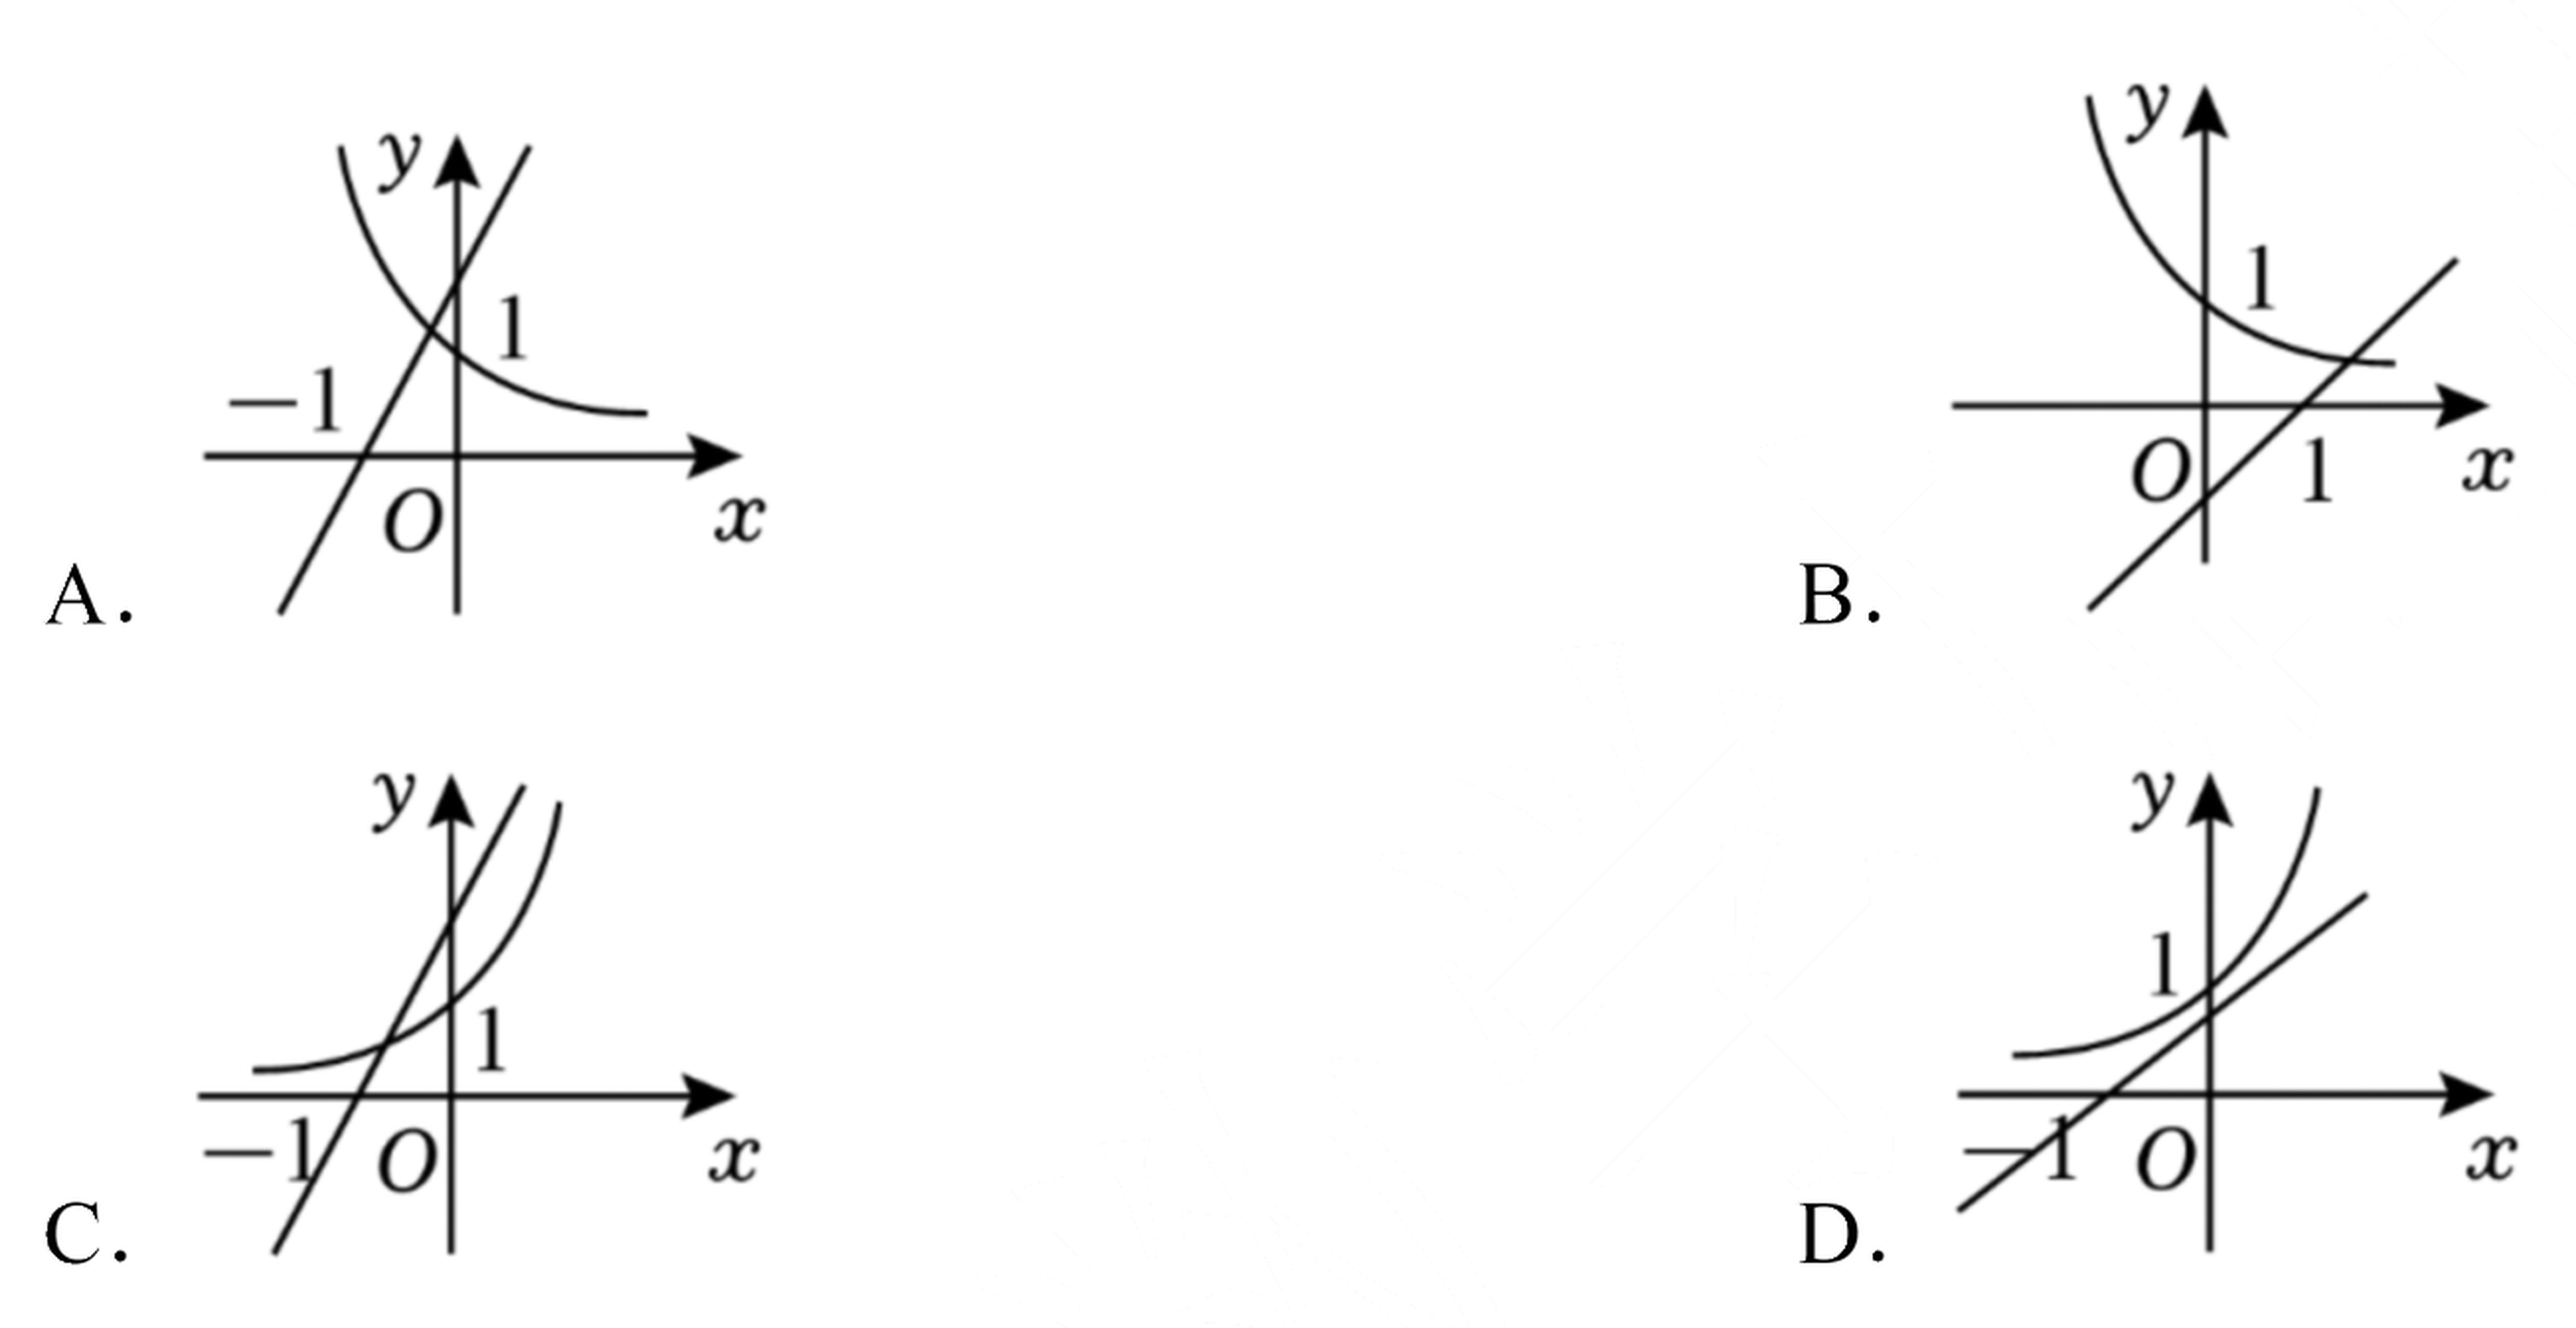
\includegraphics[width=0.80\textwidth]{figures/gao142_q15.png}
\end{center}

\ifanswer
\solbegin
\step{$A$ 中，由指数函数 $y=a^x(a>0\text{ 且 }a\neq1)$ 图像递减得 $0<a<1$，}
\step{而一次函数 $y=a(x+1)$ 的图像与 $y$ 轴交点纵坐标为 $a>1$，二者矛盾，}
\step{所以 $A$ 错；}
\step{由一次函数 $y=a(x+1)$ 的图像与 $x$ 轴交点横坐标为 $-1$，排除 $B$；}
\step{$C$ 中，由指数函数 $y=a^x(a>0\text{ 且 }a\neq1)$ 图像递减得 $a>1$，}% 原卷"递减得 a>1"自相矛盾（递减应得 0<a<1），照录
\step{而一次函数 $y=a(x+1)$ 的图像与 $y$ 轴交点纵坐标为 $a>1$，二者 $a$ 值吻合，}
\step{所以 $C$ 对；}
\step{$D$ 中，由一次函数 $y=a(x+1)$ 的图像得 $a=1$，与 $a>0$ 且 $a\neq1$ 矛盾，}
\step{所以 $D$ 错.}
\step{故选 $C$.}
\solend
\fi

\item 不等式 $\lvert x+1\rvert+\lvert 2-x\rvert\geqslant a^2-2a$ 恒成立，则 $a$ 的取值范围是\mbox{（\quad）}

\keepwithprev
A. $[-1,3]$\qquad B. $(-\infty,3]\cup[3,+\infty)$\qquad C. $(-\infty,3)$\qquad D. $(3,+\infty)$

\ifanswer
\solbegin
\step{因为 $\lvert x+1\rvert+\lvert 2-x\rvert\geqslant\lvert(x+1)+(2-x)\rvert=3$，}
\step{所以 $\lvert x+1\rvert+\lvert 2-x\rvert$ 的最小值为 3，}
\step{因为 $\lvert x+1\rvert+\lvert 2-x\rvert\geqslant a^2-2a$ 恒成立，所以只需 $a^2-2a\leqslant3$，所以 $-1\leqslant a\leqslant3$，}
\step{所以 $a$ 的取值范围为 $[-1,3]$. 故选 $A$.}
\solend
\fi

\end{enumerate}

\bigsec{三、解答题}

\begin{enumerate}
\setcounter{enumi}{16}

\item 已知集合 $A=\left\{x\mid\dfrac{x-3}{x-1}\leqslant0\right\}$，$B=\{x\mid\lvert x-1\rvert<a\}$.

(1) 若 $a=1$，求 $A\cap B$；

(2) 若 $x\in A$ 是 $x\in B$ 的充分条件，求 $a$ 的取值范围.

\ifanswer
\solbegin
\step{(1) 不等式 $\dfrac{x-3}{x-1}\leqslant0$，等价于 $(x-3)(x-1)\leqslant0$ 且 $x-1\neq0$，解得 $1<x\leqslant3$，}
\step{所以 $A=\{x\mid 1<x\leqslant3\}$，}
\step{当 $a=1$ 时，不等式 $\lvert x-1\rvert<a$ 可化为 $\lvert x-1\rvert<1$，所以 $-1<x-1<1$，}
\step{故 $0<x<2$，所以 $B=\{x\mid 0<x<2\}$，}
\step{所以 $A\cap B=\{x\mid 1<x<2\}$；}
\step{(2) 因为 $x\in A$ 是 $x\in B$ 的充分条件，所以 $A\subseteq B$，}% 子集符号原卷印带下划线 $\subseteq$，照录
\step{因为 $A=\{x\mid 1<x\leqslant3\}\neq\varnothing$，所以 $B\neq\varnothing$，故 $a>0$，}
\step{由不等式 $\lvert x-1\rvert<a$，解得 $1-a<x<1+a$，}
\step{所以 $B=\{x\mid 1-a<x<1+a\}$，所以 $\begin{cases}1-a\leqslant1\\1+a>3\end{cases}$，解得 $a>2$，}
\step{所以 $a$ 的取值范围为 $(2,+\infty)$.}
\solend
\fi

\item 计算下列式子的值（请务必书写必要的计算步骤）

(1) $27^{\frac13}+\left(\dfrac76\right)^0+\sqrt{(3-\pi)^2}$；

(2) $\lg25+\lg4+7^{\log_7 2}-\log_2 3\times\log_3 4+\log_3 9$.

\ifanswer
\solbegin
\step{(1) $27^{\frac13}+\left(\dfrac76\right)^0+\sqrt{(3-\pi)^2}=3^{3\times\frac13}+1+\lvert 3-\pi\rvert=3+1+\pi-3=\pi+1$；}
\step{(2) 原式 $=\lg(25\times4)+2-\dfrac{\lg3}{\lg2}\times\dfrac{\lg4}{\lg3}+2=\lg100+2-\dfrac{2\lg2}{\lg2}+2$}
\step{$=2+2-2+2=4$.}
\solend
\fi

\item 已知关于 $x$ 的不等式 $mx^2-(3m^2-m+2)x+6m-2\geqslant0$.

(1) 当 $m=2$ 时，求关于 $x$ 的不等式的解集；

(2) 当 $m>0$ 时，求关于 $x$ 的不等式的解集.

\ifanswer
\solbegin
\step{(1) $m=2$ 时，不等式为 $x^2-6x+5\geqslant0$，即 $(x-1)(x-5)\geqslant0$，}
\step{解得 $x\leqslant1$ 或 $x\geqslant5$，所以不等式的解集是 $\{x\mid x\leqslant1$ 或 $x\geqslant5\}$.}
\step{(2) $m>0$ 时，不等式可化为 $(mx-2)[x-(3m-1)]\geqslant0$，}
\step{即 $\left(x-\dfrac2m\right)[x-(3m-1)]\geqslant0$，}
\step{若 $m=1$，则不等式为 $(x-2)^2\geqslant0$，解得 $x\in\R$；}
\step{若 $0<m<1$，则 $\dfrac2m>3m-1$，解不等式得 $x\geqslant\dfrac2m$ 或 $x\leqslant3m-1$；}
\step{若 $m>1$，则 $\dfrac2m<3m-1$，解不等式得 $x\geqslant3m-1$ 或 $x\leqslant\dfrac2m$；}
\step{综上，$0<m<1$ 时，不等式的解集是 $\{x\mid x\leqslant3m-1$ 或 $x\geqslant\dfrac2m\}$；}
\step{$m=1$ 时，不等式的解集为 $\R$；}
\step{$m>1$ 时，不等式的解集是 $\{x\mid x\leqslant\dfrac2m$ 或 $x\geqslant3m-1\}$.}
\solend
\fi

\item 如图，某人计划用篱笆围成一个一边靠墙（墙足够长）的矩形菜园. 设菜园的长为 $x$ 米，宽为 $y$ 米.

\begin{center}
% 矩形围栏示意图取原卷 07 页截图去粉色水印、去色、LANCZOS 放大；题目配图，三版都出
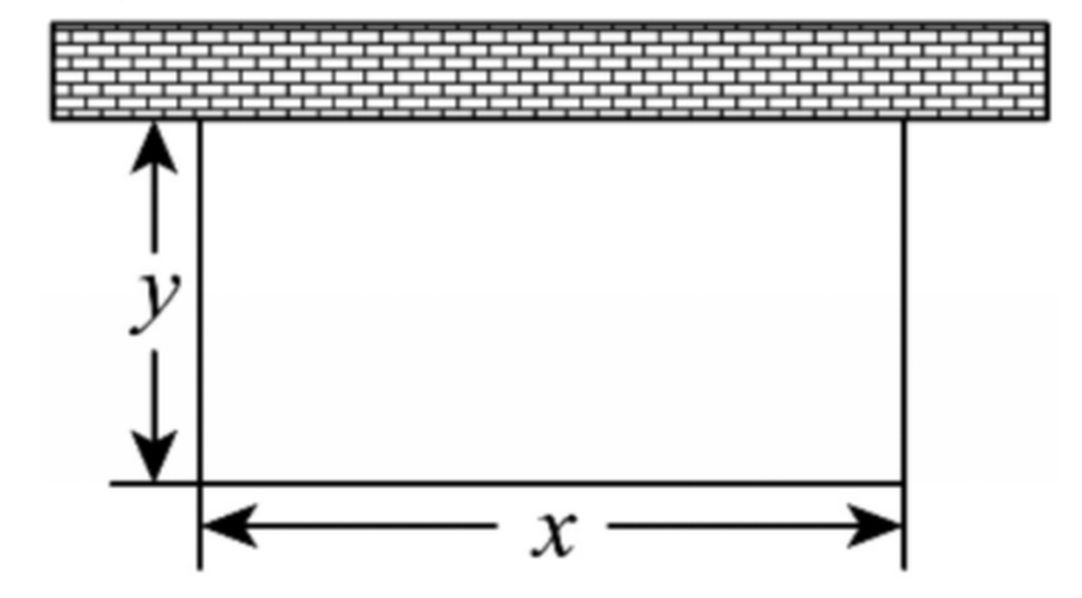
\includegraphics[width=0.42\textwidth]{figures/gao142_q20.png}
\end{center}

(1) 若菜园面积为 72 平方米，则 $x$、$y$ 为何值时，所用篱笆总长最小？

(2) 若 $x$、$y$ 满足 $x+y-xy+63=0$，则菜园面积最小为多少平方米？

\ifanswer
\solbegin
\step{(1) 由题意得，菜园的面积 $S=xy=72$，且 $x>0$，$y>0$，}
\step{所用篱笆总长 $L=x+2y$，}
\step{由基本不等式得 $x+2y\geqslant2\sqrt{x\cdot2y}=2\sqrt{2xy}=2\sqrt{2\times72}=24$，}
\step{当且仅当 $x=2y$ 时取等号，}
\step{联立 $\begin{cases}xy=72\\x=2y\end{cases}$，解得 $\begin{cases}x=12\\y=6\end{cases}$，}
\step{所以当 $x=12$，$y=6$ 时，所用篱笆总长最小；}
\step{(2) 由题意得 $x>0$，$y>0$，且满足 $x+y-xy+63=0$，即 $x+y=xy-63$，}
\step{由基本不等式得 $x+y\geqslant2\sqrt{xy}$，当且仅当 $x=y$ 时取等号，}
\step{所以 $xy-63\geqslant2\sqrt{xy}$. 令 $t=\sqrt{xy}(t>0)$，则 $xy=t^2$，}
\step{上述不等式可化为 $t^2-2t-63\geqslant0$，即 $(t-9)(t+7)\geqslant0$，}
\step{因为 $t>0$，所以 $t+7>0$，故 $t-9\geqslant0$，解得 $t\geqslant9$，所以 $\sqrt{xy}\geqslant9$，}
\step{即 $xy\geqslant81$，当且仅当 $x=y=9$ 时取等号，此时满足 $9+9-81+63=0$，}
\step{所以菜园面积最小为 81 平方米.}
\solend
\fi

\item 已知幂函数 $f(x)=(m^2-3m+3)x^m$ 的图象关于 $y$ 轴对称.

(1) 求实数 $m$ 的值；

(2) 在平面直角坐标系中作出函数 $y=\lvert f(x)-1\rvert$ 的图象；

(3) 已知点 $A(2a,y_1)$ 与点 $B(3-a,y_2)$ 都在幂函数 $y=x^2$ 的图象上. 若 $y_1<y_2$，求实数 $a$ 的取值范围.

\begin{center}
% 空白坐标网格取原卷 08 页截图去粉色水印、去色、LANCZOS 放大；题目配图，三版都出
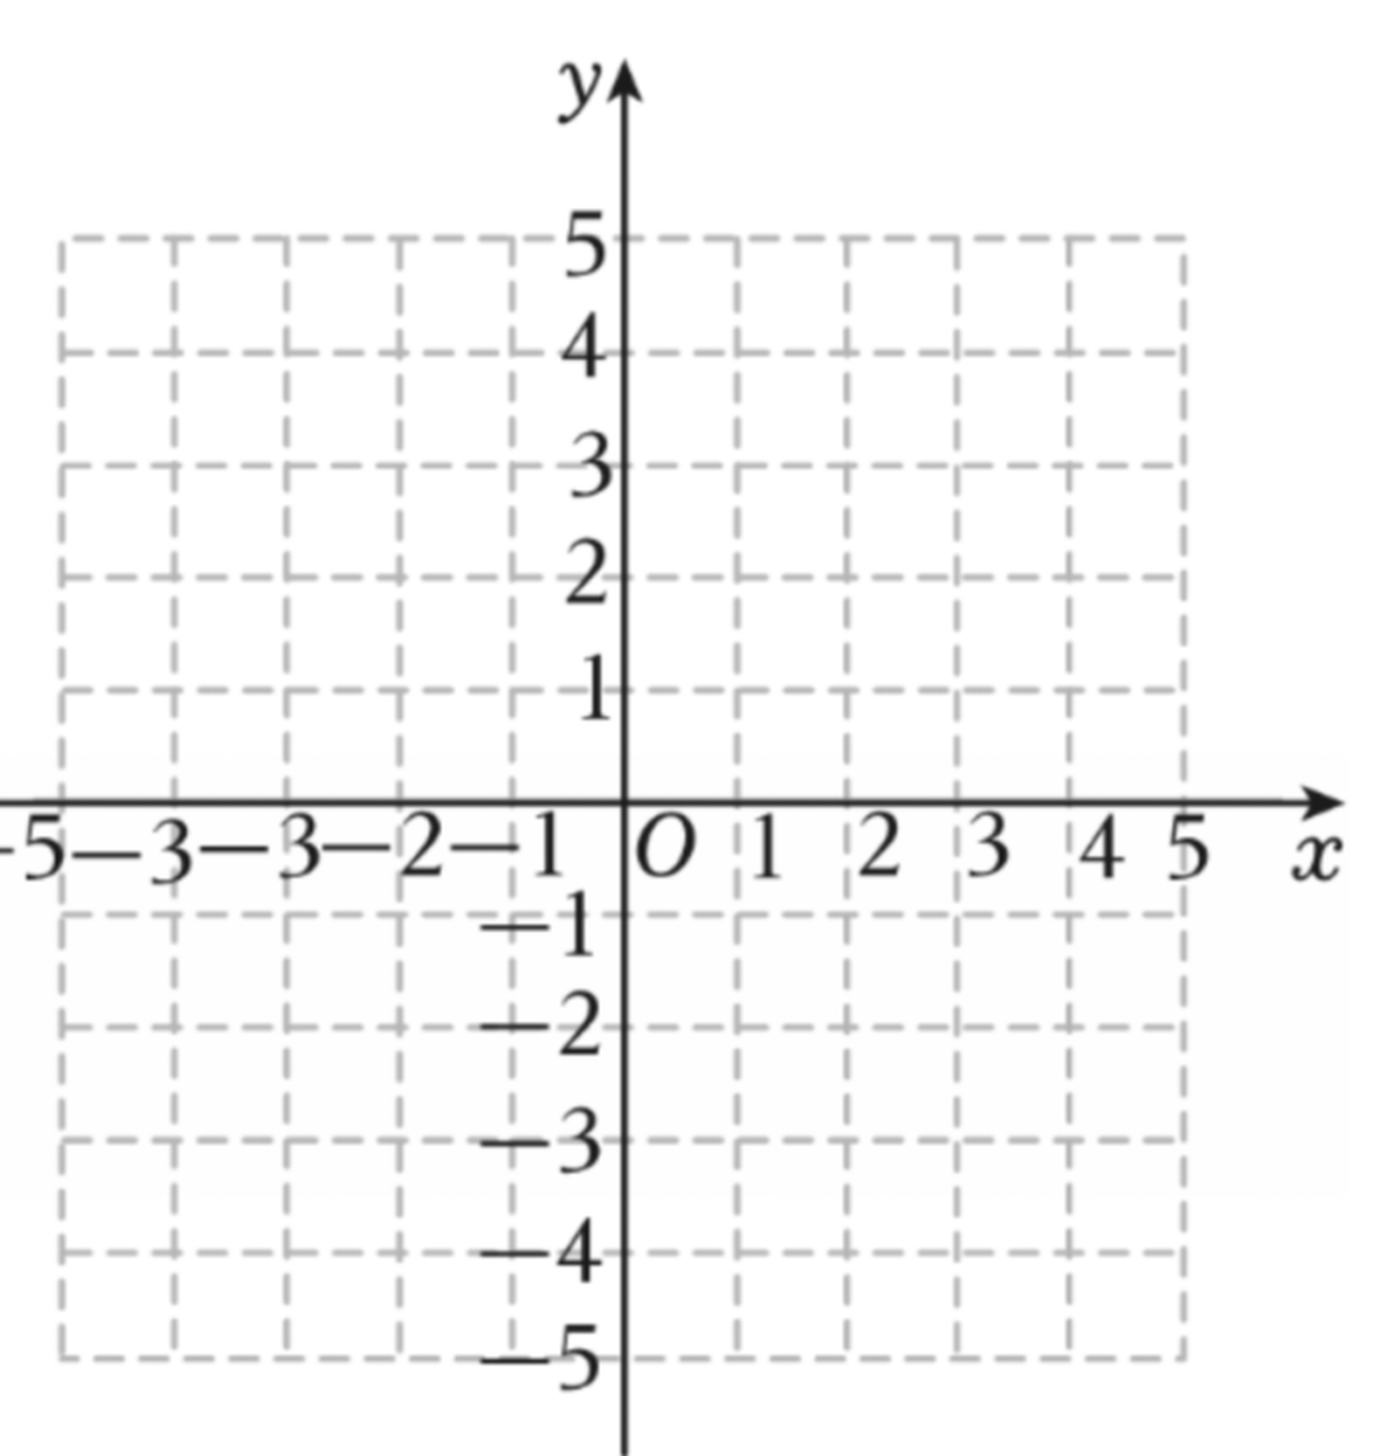
\includegraphics[width=0.52\textwidth]{figures/gao142_q21_grid.png}
\end{center}

\ifanswer
\solbegin
\step{(1) 由题意幂函数 $f(x)=(m^2-3m+3)x^m$，}
\step{故 $m^2-3m+3=1$，解得 $m=1$ 或 $m=2$，}
\step{又 $f(x)$ 图象关于 $y$ 轴对称，即 $f(x)$ 是偶函数，}
\step{当 $m=1$ 时，$f(x)=x$ 是奇函数，不满足条件，舍去；}
\step{当 $m=2$ 时，$f(x)=x^2$ 是偶函数，满足条件，故 $m=2$；}
\step{(2) 由 (1) 得，$\lvert f(x)-1\rvert=\lvert x^2-1\rvert$，}
\step{先画 $y=x^2-1$，开口向上的抛物线，顶点 $(0,-1)$，零点 $x=\pm1$，}
\step{再将 $x$ 轴下方的部分沿 $x$ 轴翻折到上方即为 $y=\lvert x^2-1\rvert$ 的图象，}
\step{图象如图所示.}
\par{\leftskip=0pt
\begin{center}
% 抛物线图象取原卷 09 页截图去粉色水印、去色、LANCZOS 放大；解析所附配图，仅答案版出
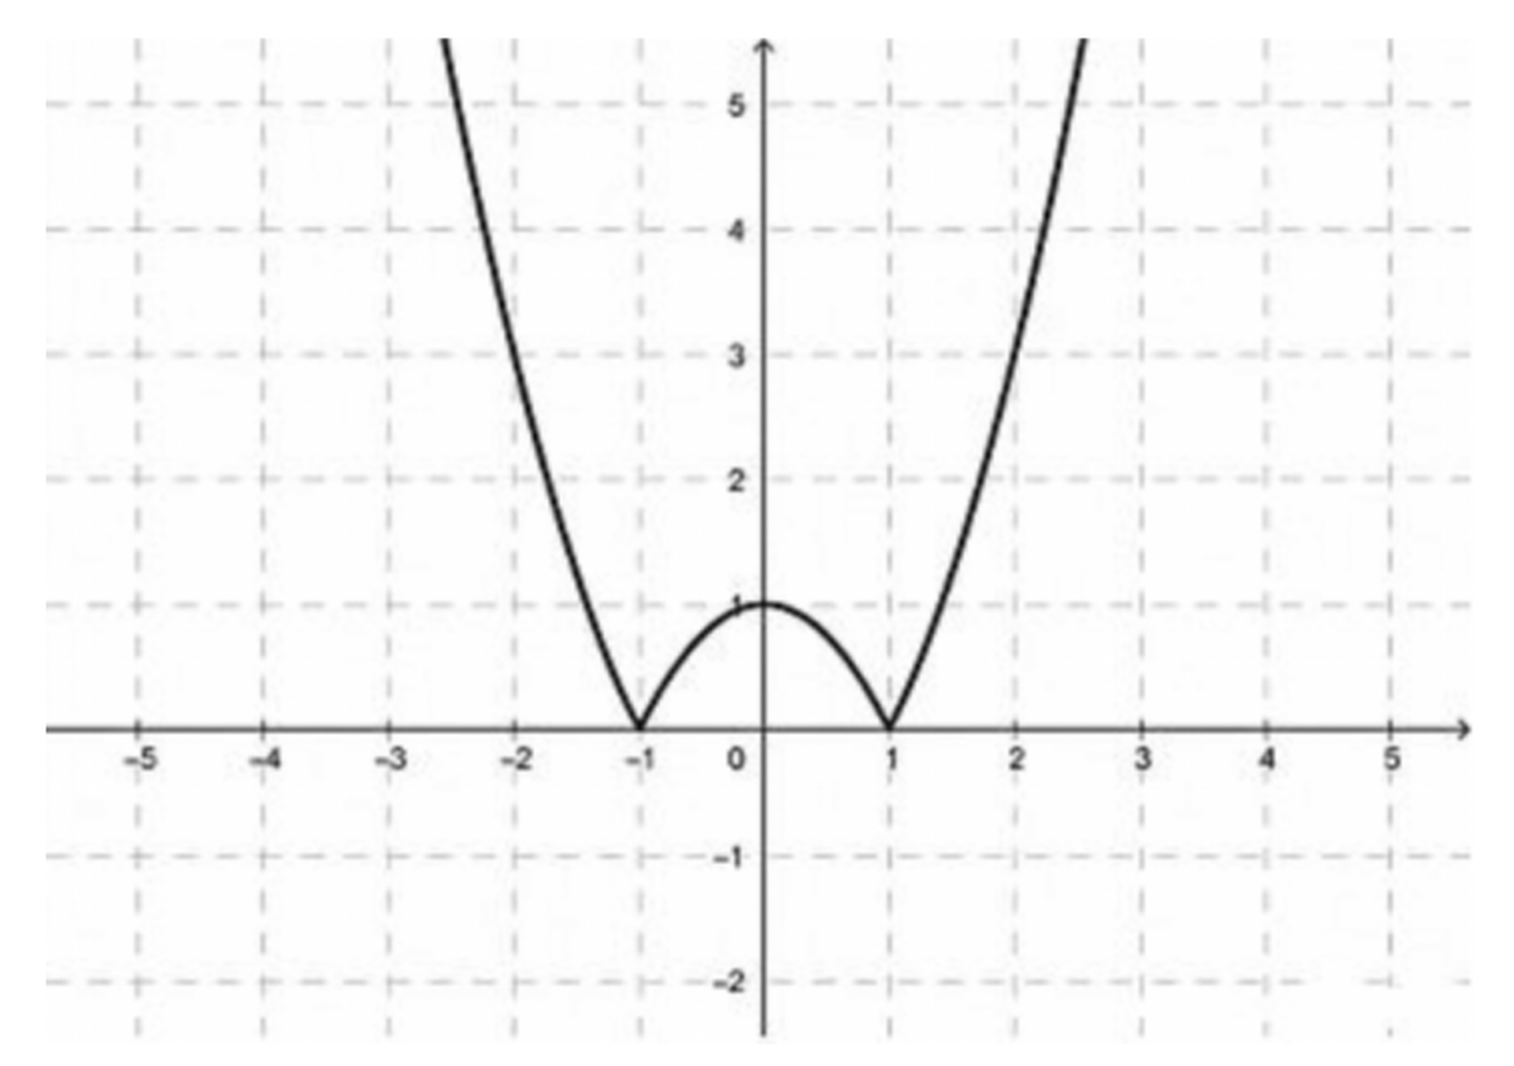
\includegraphics[width=0.55\textwidth]{figures/gao142_q21_para.png}
\end{center}}
\step{(3) 由题意得，$y_1=(2a)^2$，$y_2=(3-a)^2$，}
\step{$y_1<y_2$，即有 $(2a)^2<(3-a)^2$，化简整理得 $(a+3)(a-1)<0$，}
\step{解得实数 $a$ 的取值范围为 $(-3,1)$.}
\solend
\fi

\end{enumerate}

\end{document}
"
% 紧凑版：xelatex "\def\iscompact{1}% 高一142_群峰高级中学_期中.tex
%   —— 高一上数学"2026-2027 年群峰高级中学高一上期中"（试卷版/答案版）
% 试卷版：xelatex 高一142_群峰高级中学_期中.tex
% 答案版：xelatex "\def\isanswer{1}\input{高一142_群峰高级中学_期中.tex}"
% 紧凑版：xelatex "\def\iscompact{1}\input{高一142_群峰高级中学_期中.tex}"
%
% ① 原始材料：微信公众号"魔都数学加油站"文章，连载"27学年高一142"，原文标题
% "27学年高一142——2026-2027年上海市群峰高级中学高一上期中"；
% 原文链接：https://mp.weixin.qq.com/s/cc7wnuP4Pk3OjNDV6ihB9A。
% 正文为 9 张 PNG 页（01、02、04、06、07、08、09 为 2560x3620；03、05 为 4762x6735，
% 同一篇各页分辨率不同，逐页按各自分辨率裁图核对），题目下印有【答案】或【解析】，为讲评版。
% 题目、解析均据原图转录；卷面粉红色水印"魔都数学加油站"及公众号页脚未录入。
% 全卷 4 幅插图：第 15 题四幅坐标函数图像选项（04 页，2x2 合并为一张）、
% 第 20 题矩形围栏示意图（07 页）、第 21 题 (2) 空白坐标网格（08 页）、
% 第 21 题抛物线图象（09 页，解析所附图）；均取原卷截图去粉色水印、LANCZOS 放大。
% 题目配图三版都出、解析配图仅答案版出。
%
% 卷首标题：原卷印作"2026-2027 年群峰高级中学高一上期中"（公众号标题中的"上海市"
% 卷面标题行没有，本稿照卷面），年份区间按全稿惯例排 en dash；原卷未印副标题，
% 本卷为期中卷、跨集合与常用逻辑用语／不等式／函数三章，按题目内容补出
% "集合与常用逻辑用语、不等式、函数"（头注说明，与同期中卷口径相同）。
%
% 题号体例：本卷共 19 题——一、填空题 3—12（10 题）、二、选择题 13—16（4 题）、
% 三、解答题 17—21（5 题）。三节分别 \setcounter{enumi}{2}／{12}／{16}。
% 原卷从第 3 题起、无第 1、2 题，本稿保留原题号。
%
% ② 与原卷的排版差异：
%   ① 原文从第 3 题起，本稿保留原题号；原卷未印副标题，本稿按"知识模块"口径补出；
%   ② 逐题答案口径：Q14 原卷把答案 D 印在题干括号内、且题目下无【解析】，本稿括号
%      留空 \mbox{（\quad）}、另提 \ans{D}；Q13／Q15／Q16 答案在【解析】末句"故选 …"
%      （分别为 C／C／A），题干括号留空、不另提 \ans{}；其余各题（Q3—Q12、
%      Q17—Q21）题目下印【解析】、答案融在解析中，不另提 \ans{}；全卷仅 Q14 一处 \ans{}；
%      答案版【答案】/【解析】标记数 = 19（1 个 \ans + 18 个 \solbegin）= 全卷题数；
%   ③ 原卷填空横线按全稿惯例排 \blankline[4.4em]；选择题括号排 \mbox{（\quad）}、
%      每个选项段前按惯例加 \keepwithprev（Q15 四幅图那一枚放在 \begin{center} 之前）；
%      解答题不留作答区、不加 \anspace（原卷为讲评版，与 129／131／132／133／136／140 同）；
%   ④ 原卷数集斜体 $R$（Q5、Q7、Q19、Q21 解析等）按全稿惯例统一改 \R；空集记号
%      \varnothing；绝对值排 \lvert…\rvert，集合描述竖线排 \mid；不等号按全稿惯例
%      排 \leqslant／\geqslant；
%   ⑤ 4 幅插图：Q15 四幅坐标函数图象选项合并裁为一张 \includegraphics（题前
%      \needvspace{9cm}）；Q15 是"二、选择题"节内带大图块的第 3 题（Q13、Q14 在前
%      且无图），另在 \bigsec{二、选择题} 之前加 \needvspace{11cm} 连节标题一起量
%      ——守卫必须放在 \bigsec 之前，放标题之后会让"二、选择题"孤立在页末
%      （B 类，照 高一26／40／59／136／140 成例）；Q20 围栏图与 Q21 网格图置于题干
%      之后（三版都出），Q21 抛物线图置于答案版解析 (2) 与 (3) 之间（仅答案版出）；
%   ⑥ 子题标号按原卷排半角 (1)(2)(3)（与 140／141 同期中卷口径相同）；括注全角／
%      半角逐处照录：Q3"（用含有 m 的代数式表示）"、Q6"（舍）"、Q10"（万元）"、
%      Q18"（请务必书写必要的计算步骤）"、Q20"（墙足够长）"印全角；Q15
%      "$y=a^x(a>0 且 a\neq1)$"、Q10"$y=x^a(a 为常数)$"、Q20"$t=\sqrt{xy}(t>0)$"
%      等数学式内括注印半角；数学式内 CJK 用 \text{…}（否则 FONTCHK 报缺字）；
%   ⑦ 数学式内半角逗号照录（如 Q6"$ax-1=0,a\in\R$"、Q9"$b=2+\sqrt2,a=\sqrt2+1$"、
%      Q16 区间 "$[-1,3]$"、Q21"$y_1<y_2$，即 $(2a)^2<(3-a)^2$" 等）；原卷行末
%      西文句点照录（Q7"(-3,5)."、Q10"125（万元）."、Q19 题干句点、Q20 题干
%      "矩形菜园."与"宽为 y 米."、Q21 题干"对称." 等）；行中全角逗号、分号照录；
%   ⑧ 题干中的中文弯引号：本卷题干与解析通篇未出现中文弯引号，故无此项；
%      圈数字 ①②③ 亦未出现（子题用 (1)(2)(3)）；
%   ⑨ 原卷"图像／图象"两种写法混用，逐处放大核对并照录：Q4 题干与解析作"图象"、
%      Q7 解析作"图象"、Q8 题干作"图像"而解析作"图象"、Q15 题干与解析通篇作
%      "图像"、Q21 题干与解析通篇作"图象"；
%   ⑩ 原卷无红色加粗标签（【解析】均黑色印刷；逐页扫描深红像素为 0），故本卷未用
%      \stepm；黑色常规分步标签（"A 中""C 中""D 中""(1)(2)(3)" 等）按普通 \step
%      行内文字照录；
%   ⑪ 跨页续印按题合并，明细见 ⑥。
%
% ③ 行数复核：一条 \step = 原卷解析的一个印刷行，cases 块作一个印刷行计。逐题数 \step
%   条数，合计 98 条（Q3：1；Q4：2；Q5：3；Q6：4；Q7：5；Q8：2；Q9：4；Q10：3；
%   Q11：4；Q12：3；Q13：5；Q14：0；Q15：10；Q16：4；Q17：10；Q18：3；
%   Q19：10；Q20：13；Q21：12），与原卷印刷行逐题相等。Q14 只把答案印在题干括号、
%   无【解析】，提 \ans{D}、不计入 \step 账；答案版标记数 = 19（1 个 \ans + 18 个
%   \solbegin）= 全卷题数。
%
% ④ 判别式字形：全卷判别式共 3 处——第 7 题【解析】"即判别式△<0"、
%   "即△=(a-1)^2-4×1×4<0" 两处原卷印扁等边三角 $\triangle$，
%   第 11 题【解析】cases 块"△=4a^2-4(a+6)≥0" 一处原卷印等腰偏高的高三角 $\Delta$；
%   逐处放大核对，两形不同、全卷混用，本稿逐处照录不统一（参照 高一141 头注④口径）。
%   子集符号：全卷共 3 处——第 6 题题干"若 B⊆A"、第 6 题【解析】"因为 B⊆A"、
%   第 17 题【解析】(2)"所以 A⊆B"，逐处放大核对，原卷三处均印带下划线的
%   $\subseteq$（不是单线 $\subset$），本稿一律照录 \subseteq；全卷未出现 \subset。
%
% ⑤ 原卷存疑照录（均照录未改，正文对应处另有 % 注）：
%   第 14 题题干括号内原卷印答案 D（非留空），且题目下无【解析】，按"答案印括号且
%      无解析"口径括号留空、另提 \ans{D}；
%   第 15 题【解析】"C 中，由指数函数 … 图像递减得 a>1" 中"递减"与"a>1"
%      自相矛盾（递减应得 0<a<1，疑为"递增"之误），照录；
%   第 16 题选项 B 作 $(-\infty,3]\cup[3,+\infty)$，两端区间并起即全体实数、
%      与正确答案 $[-1,3]$ 不成干扰项（疑为 $(-\infty,-1]\cup[3,+\infty)$ 之误），照录；
%   第 21 题 (2) 空白坐标网格的 x 轴刻度原卷印作"-5 -3 -3 -2 -1 0 1 2 3 4 5"
%      （"-3"重复，疑为"-4"之误），系插图中的印刷内容，取原卷截图照录、不改图。
%
% ⑥ 跨页续印说明：Q7 题干与解析首行在 01 页、解析续至 02 页；Q11 题干与解析
%   4 行在 03 页；Q13 解析前 4 行在 03 页、末句"故选 C."续至 04 页；Q15 题干与
%   四幅图在 04 页、解析前 8 行在 04 页、末 2 行续至 05 页；Q17 解析前 7 行在
%   05 页、后 3 行续至 06 页；Q19 解析前 5 行在 06 页、后 5 行续至 07 页；
%   Q20 解析前 9 行在 07 页、后 4 行续至 08 页；Q21 解析 (1)(2) 9 行在 08 页、
%   抛物线图与 (3) 3 行续至 09 页；本稿按题连排，不丢行。三版切页审计结论见
%   编译自验回报（切页守卫见 ②⑤）。
%
\documentclass[a4paper,11pt]{article}
\usepackage{common}

\begin{document}

\examtitlest[3]{2026--2027 年群峰高级中学高一上期中}{集合与常用逻辑用语、不等式、函数}

\bigsec{一、填空题}

\begin{enumerate}
\setcounter{enumi}{2}

\item 已知 $\log_2 3=m$，则 $\log_3 6=$\blankline[4.4em]（用含有 $m$ 的代数式表示）.

\ifanswer
\solbegin
\step{$\log_3 6=\dfrac{\log_2 6}{\log_2 3}=\dfrac{\log_2 2+\log_2 3}{\log_2 3}=\dfrac{1+m}{m}=\dfrac1m+1$.}
\solend
\fi

\item 若指数函数 $y=a^x$ 的图象经过点 $(3,27)$，则 $a$ 的值为\blankline[4.4em].

\ifanswer
\solbegin
\step{因为指数函数 $y=a^x$ 的图象经过点 $(3,27)$，}
\step{所以 $a^3=27=3^3$，所以 $a=3$.}
\solend
\fi

\item 不等式 $(2x+1)^{\frac13}<(3-x)^{\frac13}$ 的解集为\blankline[4.4em].

\ifanswer
\solbegin
\step{因为幂函数 $f(t)=t^{\frac13}$ 在 $\R$ 上严格增，}
\step{所以原不等式等价于 $2x+1<3-x$，解得 $x<\dfrac23$，}
\step{因此原不等式的解集为 $\left(-\infty,\dfrac23\right)$.}
\solend
\fi

\item 设集合 $A=\{1,-2\}$，$B=\{x\mid ax-1=0,a\in\R\}$，若 $B\subseteq A$，则 $a$ 的值为\blankline[4.4em].% 子集符号原卷印带下划线 $\subseteq$，照录

\ifanswer
\solbegin
\step{因为 $B\subseteq A$，所以 $B=\varnothing$ 或 $\{-2\}$ 或 $\{1\}$ 或 $\{1,-2\}$（舍），}% 子集符号原卷印带下划线 $\subseteq$，照录
\step{若 $B=\varnothing$，则 $a=0$；若 $B=\{1\}$，则 $a=1$；}
\step{若 $B=\{-2\}$，则 $-2a=1$，解得 $a=-\dfrac12$；}
\step{综上，$a=0$ 或 $1$ 或 $-\dfrac12$.}
\solend
\fi

\item 不等式 $x^2+(a-1)x+4>0$ 在 $\R$ 上恒成立，则实数 $a$ 的取值范围是\blankline[4.4em].

\ifanswer
\solbegin
\step{不等式 $x^2+(a-1)x+4>0$，对应的二次函数为 $y=x^2+(a-1)x+4$，}
\step{因此函数图象开口向上，要使不等式对任意实数 $x$ 恒成立，}
\step{需二次函数图象与 $x$ 轴无交点，即判别式 $\triangle<0$，}% 判别式原卷印扁等边三角 $\triangle$，照录
\step{即 $\triangle=(a-1)^2-4\times1\times4<0$，整理得 $a^2-2a-15<0$，}% 判别式原卷印扁等边三角 $\triangle$，照录
\step{解得 $-3<a<5$，故实数 $a$ 的取值范围是 $(-3,5)$.}
\solend
\fi

\item 函数 $f(x)=(5x-3)^a$ 的图像恒过点\blankline[4.4em].% 题干作"图像"、解析作"图象"，原卷混用，逐处照录

\ifanswer
\solbegin
\step{令 $5x-3=1$ 得 $x=\dfrac45$，此时 $f\left(\dfrac45\right)=\left(5\times\dfrac45-3\right)^a=1$，}
\step{所以 $f(x)$ 的图象恒过 $\left(\dfrac45,1\right)$.}
\solend
\fi

\item 若 $a>0$，$b>0$ 且 $\dfrac1a+\dfrac2b=1$，则 $a+b$ 的最小值为\blankline[4.4em].

\ifanswer
\solbegin
\step{因为 $a>0$，$b>0$，$\dfrac1a+\dfrac2b=1$，}
\step{所以 $a+b=(a+b)\left(\dfrac1a+\dfrac2b\right)=1+\dfrac{2a}{b}+\dfrac{b}{a}+2\geqslant3+2\sqrt{\dfrac{2a}{b}\cdot\dfrac{b}{a}}=3+2\sqrt2$，}
\step{当且仅当 $\dfrac{2a}{b}=\dfrac{b}{a}$，即 $b=2+\sqrt2,a=\sqrt2+1$ 时取等号，}
\step{故 $a+b$ 的最小值为 $3+2\sqrt2$.}
\solend
\fi

\item 某药厂研制出一种新型药剂，投放市场后其广告投入 $x$（万元）与药品利润 $y$（万元）存在的关系为 $y=x^a(a\text{ 为常数})$，其中 $x$ 不超过 5 万元. 已知去年投入广告费用为 3 万元时，药品利润为 27 万元，若今年投入广告费用 5 万元，预计今年药品利润为\blankline[4.4em]万元.

\ifanswer
\solbegin
\step{由已知投入广告费用为 3 万元时，药品利润为 27 万元，}
\step{代入 $y=x^a$ 中，即 $3^a=27$，解得 $a=3$，故函数关系式为 $y=x^3$，}
\step{所以当 $x=5$ 时，$y=125$（万元）.}
\solend
\fi

\item 已知方程 $x^2+2ax+a+6=0$ 的两根分别是 $x_1$ 和 $x_2$，且满足 $\dfrac1{x_1}+\dfrac1{x_2}<0$，则实数 $a$ 的取值范围是\blankline[4.4em].

\ifanswer
\solbegin
\step{由于方程 $x^2+2ax+a+6=0$ 的两根分别是 $x_1$ 和 $x_2$，}
\step{则 $\begin{cases}\Delta=4a^2-4(a+6)\geqslant0\\x_1+x_2=-2a\\x_1x_2=a+6\end{cases}$，解得 $a\geqslant3$ 或 $a\leqslant-2$.}% 判别式原卷印等腰偏高的高三角 $\Delta$，照录（与第 7 题扁等边 $\triangle$ 两形混用）
\step{又 $\dfrac1{x_1}+\dfrac1{x_2}<0$，即 $\dfrac{x_1+x_2}{x_1\cdot x_2}<0$，故 $\dfrac{-2a}{a+6}<0$，解得 $a<-6$ 或 $a>0$.}
\step{综上，$a$ 的取值范围是 $(-\infty,-6)\cup[3,+\infty)$.}
\solend
\fi

\item 已知 $b>a>1$，若 $\log_a b-\log_b a=\dfrac32$，$a^b=b^a$，则 $a-b=$\blankline[4.4em].

\ifanswer
\solbegin
\step{因为 $b>a>1$，所以 $\log_a b>1$，}
\step{由 $\log_a b-\log_b a=\log_a b-\dfrac{1}{\log_a b}=\dfrac32$，解得 $\log_a b=2$ 即 $b=a^2$，}
\step{因为 $a^b=b^a=a^{2a}$，所以 $b=2a=a^2$，所以 $a=2$，$b=4$，则 $a-b=-2$.}
\solend
\fi

\end{enumerate}

% 第 15 题四幅图是"二、选择题"节内的大图块；守卫须放在 \bigsec 之前连节标题一起量
\needvspace{11cm}
\bigsec{二、选择题}

\begin{enumerate}
\setcounter{enumi}{12}

\item 若 $a>b$，$c<0$，则下列不等式正确的是\mbox{（\quad）}

\keepwithprev
A. $ab>bc$\qquad B. $a+c<b+c$\qquad C. $ac^2>bc^2$\qquad D. $\dfrac ac>\dfrac bc$

\ifanswer
\solbegin
\step{因为 $a>b$，$c<0$，取 $b=0$，则 $ab=bc=0$，故 $A$ 错误；}
\step{由于 $a>b$，所以 $a+c>b+c$，故 $B$ 错误；}
\step{由 $c<0$ 得 $c^2>0$，所以 $ac^2>bc^2$，故 $C$ 正确；}
\step{由于 $a>b$ 且 $c<0$，所以 $\dfrac ac<\dfrac bc$，故 $D$ 错误.}
\step{故选 $C$.}
\solend
\fi

\item 若 $x>0$，$y>0$，则下列各式中，恒成立的是\mbox{（\quad）}% 原卷题干括号内印答案 D、且题目下无【解析】，本稿括号留空、另提 \ans{D}

\keepwithprev
A. $\lg x+\lg y=\lg(x+y)$\qquad B. $\lg x^2=(\lg x)^2$

C. $\dfrac{\lg x}{\lg y}=\lg(x-y)$\qquad D. $\lg x^{\frac1n}=\dfrac{\lg x}{n}$

\ifanswer
\ans{$D$}
\fi

% 第 15 题四幅坐标函数图象选项是一整块，守卫放在 \item 之前
\needvspace{9cm}
\item 在同一平面直角坐标系中，指数函数 $y=a^x(a>0\text{ 且 }a\neq1)$ 和一次函数 $y=a(x+1)$ 的图像关系可能是\mbox{（\quad）}

\keepwithprev
\begin{center}
% 四幅坐标函数图象选项取原卷 04 页截图去粉色水印、去色，按原卷 2x2 排布合并为一张
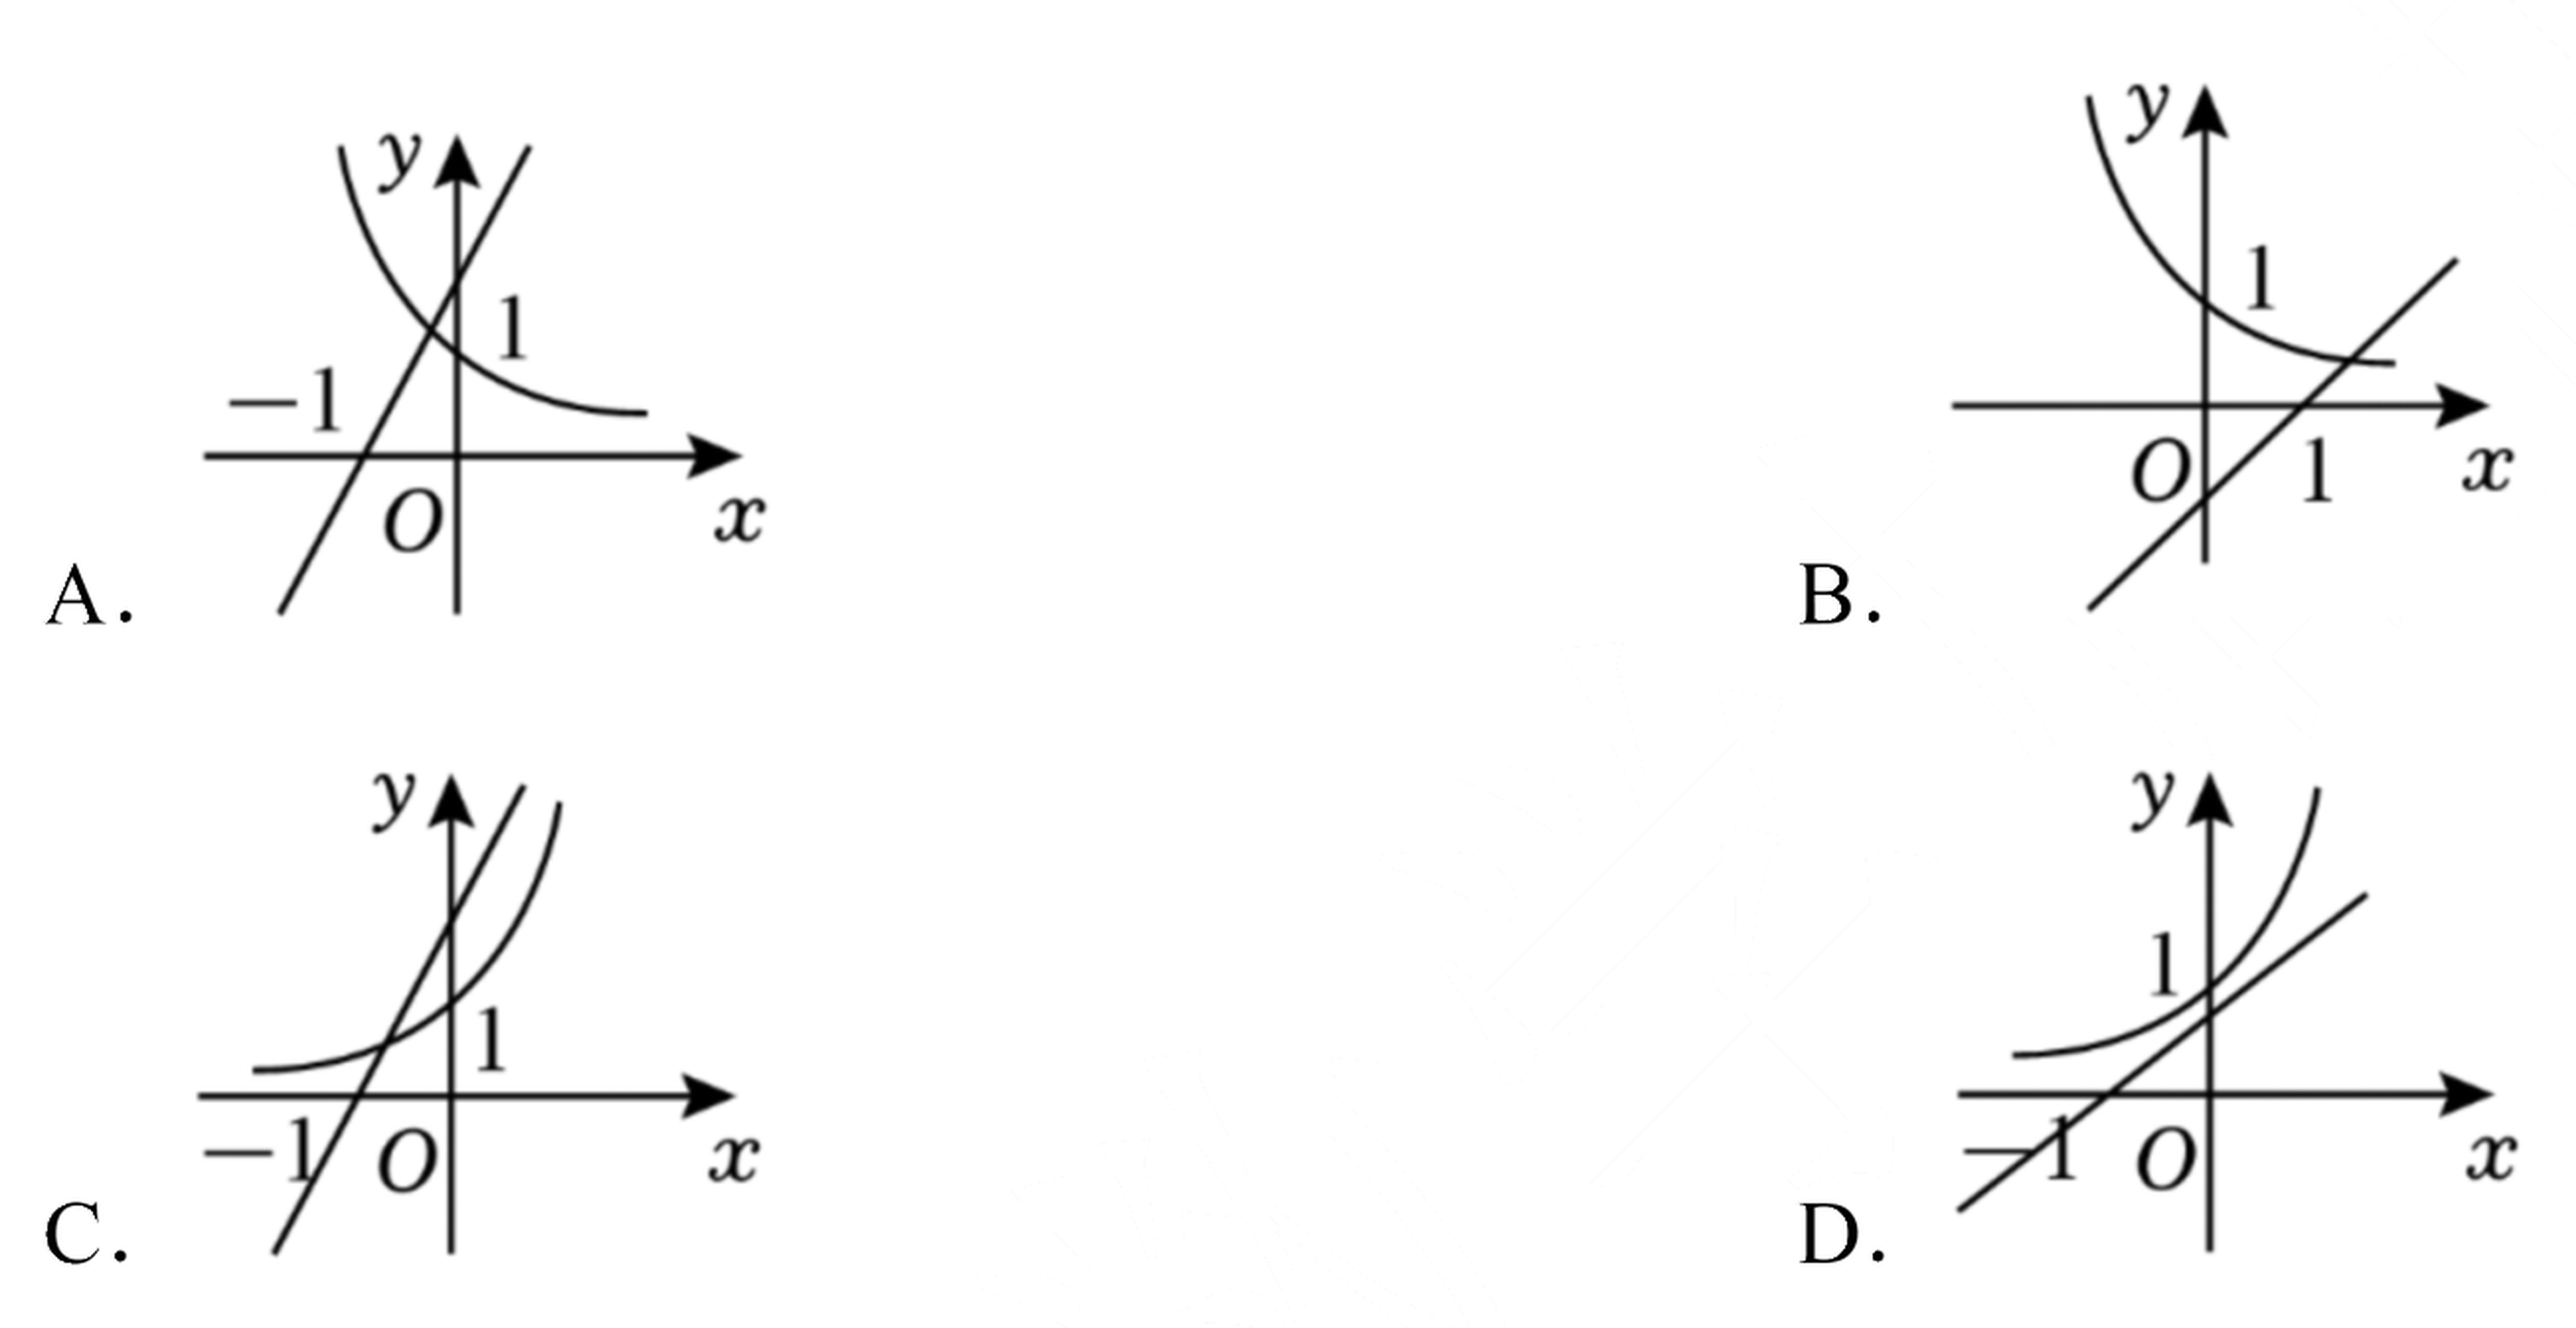
\includegraphics[width=0.80\textwidth]{figures/gao142_q15.png}
\end{center}

\ifanswer
\solbegin
\step{$A$ 中，由指数函数 $y=a^x(a>0\text{ 且 }a\neq1)$ 图像递减得 $0<a<1$，}
\step{而一次函数 $y=a(x+1)$ 的图像与 $y$ 轴交点纵坐标为 $a>1$，二者矛盾，}
\step{所以 $A$ 错；}
\step{由一次函数 $y=a(x+1)$ 的图像与 $x$ 轴交点横坐标为 $-1$，排除 $B$；}
\step{$C$ 中，由指数函数 $y=a^x(a>0\text{ 且 }a\neq1)$ 图像递减得 $a>1$，}% 原卷"递减得 a>1"自相矛盾（递减应得 0<a<1），照录
\step{而一次函数 $y=a(x+1)$ 的图像与 $y$ 轴交点纵坐标为 $a>1$，二者 $a$ 值吻合，}
\step{所以 $C$ 对；}
\step{$D$ 中，由一次函数 $y=a(x+1)$ 的图像得 $a=1$，与 $a>0$ 且 $a\neq1$ 矛盾，}
\step{所以 $D$ 错.}
\step{故选 $C$.}
\solend
\fi

\item 不等式 $\lvert x+1\rvert+\lvert 2-x\rvert\geqslant a^2-2a$ 恒成立，则 $a$ 的取值范围是\mbox{（\quad）}

\keepwithprev
A. $[-1,3]$\qquad B. $(-\infty,3]\cup[3,+\infty)$\qquad C. $(-\infty,3)$\qquad D. $(3,+\infty)$

\ifanswer
\solbegin
\step{因为 $\lvert x+1\rvert+\lvert 2-x\rvert\geqslant\lvert(x+1)+(2-x)\rvert=3$，}
\step{所以 $\lvert x+1\rvert+\lvert 2-x\rvert$ 的最小值为 3，}
\step{因为 $\lvert x+1\rvert+\lvert 2-x\rvert\geqslant a^2-2a$ 恒成立，所以只需 $a^2-2a\leqslant3$，所以 $-1\leqslant a\leqslant3$，}
\step{所以 $a$ 的取值范围为 $[-1,3]$. 故选 $A$.}
\solend
\fi

\end{enumerate}

\bigsec{三、解答题}

\begin{enumerate}
\setcounter{enumi}{16}

\item 已知集合 $A=\left\{x\mid\dfrac{x-3}{x-1}\leqslant0\right\}$，$B=\{x\mid\lvert x-1\rvert<a\}$.

(1) 若 $a=1$，求 $A\cap B$；

(2) 若 $x\in A$ 是 $x\in B$ 的充分条件，求 $a$ 的取值范围.

\ifanswer
\solbegin
\step{(1) 不等式 $\dfrac{x-3}{x-1}\leqslant0$，等价于 $(x-3)(x-1)\leqslant0$ 且 $x-1\neq0$，解得 $1<x\leqslant3$，}
\step{所以 $A=\{x\mid 1<x\leqslant3\}$，}
\step{当 $a=1$ 时，不等式 $\lvert x-1\rvert<a$ 可化为 $\lvert x-1\rvert<1$，所以 $-1<x-1<1$，}
\step{故 $0<x<2$，所以 $B=\{x\mid 0<x<2\}$，}
\step{所以 $A\cap B=\{x\mid 1<x<2\}$；}
\step{(2) 因为 $x\in A$ 是 $x\in B$ 的充分条件，所以 $A\subseteq B$，}% 子集符号原卷印带下划线 $\subseteq$，照录
\step{因为 $A=\{x\mid 1<x\leqslant3\}\neq\varnothing$，所以 $B\neq\varnothing$，故 $a>0$，}
\step{由不等式 $\lvert x-1\rvert<a$，解得 $1-a<x<1+a$，}
\step{所以 $B=\{x\mid 1-a<x<1+a\}$，所以 $\begin{cases}1-a\leqslant1\\1+a>3\end{cases}$，解得 $a>2$，}
\step{所以 $a$ 的取值范围为 $(2,+\infty)$.}
\solend
\fi

\item 计算下列式子的值（请务必书写必要的计算步骤）

(1) $27^{\frac13}+\left(\dfrac76\right)^0+\sqrt{(3-\pi)^2}$；

(2) $\lg25+\lg4+7^{\log_7 2}-\log_2 3\times\log_3 4+\log_3 9$.

\ifanswer
\solbegin
\step{(1) $27^{\frac13}+\left(\dfrac76\right)^0+\sqrt{(3-\pi)^2}=3^{3\times\frac13}+1+\lvert 3-\pi\rvert=3+1+\pi-3=\pi+1$；}
\step{(2) 原式 $=\lg(25\times4)+2-\dfrac{\lg3}{\lg2}\times\dfrac{\lg4}{\lg3}+2=\lg100+2-\dfrac{2\lg2}{\lg2}+2$}
\step{$=2+2-2+2=4$.}
\solend
\fi

\item 已知关于 $x$ 的不等式 $mx^2-(3m^2-m+2)x+6m-2\geqslant0$.

(1) 当 $m=2$ 时，求关于 $x$ 的不等式的解集；

(2) 当 $m>0$ 时，求关于 $x$ 的不等式的解集.

\ifanswer
\solbegin
\step{(1) $m=2$ 时，不等式为 $x^2-6x+5\geqslant0$，即 $(x-1)(x-5)\geqslant0$，}
\step{解得 $x\leqslant1$ 或 $x\geqslant5$，所以不等式的解集是 $\{x\mid x\leqslant1$ 或 $x\geqslant5\}$.}
\step{(2) $m>0$ 时，不等式可化为 $(mx-2)[x-(3m-1)]\geqslant0$，}
\step{即 $\left(x-\dfrac2m\right)[x-(3m-1)]\geqslant0$，}
\step{若 $m=1$，则不等式为 $(x-2)^2\geqslant0$，解得 $x\in\R$；}
\step{若 $0<m<1$，则 $\dfrac2m>3m-1$，解不等式得 $x\geqslant\dfrac2m$ 或 $x\leqslant3m-1$；}
\step{若 $m>1$，则 $\dfrac2m<3m-1$，解不等式得 $x\geqslant3m-1$ 或 $x\leqslant\dfrac2m$；}
\step{综上，$0<m<1$ 时，不等式的解集是 $\{x\mid x\leqslant3m-1$ 或 $x\geqslant\dfrac2m\}$；}
\step{$m=1$ 时，不等式的解集为 $\R$；}
\step{$m>1$ 时，不等式的解集是 $\{x\mid x\leqslant\dfrac2m$ 或 $x\geqslant3m-1\}$.}
\solend
\fi

\item 如图，某人计划用篱笆围成一个一边靠墙（墙足够长）的矩形菜园. 设菜园的长为 $x$ 米，宽为 $y$ 米.

\begin{center}
% 矩形围栏示意图取原卷 07 页截图去粉色水印、去色、LANCZOS 放大；题目配图，三版都出
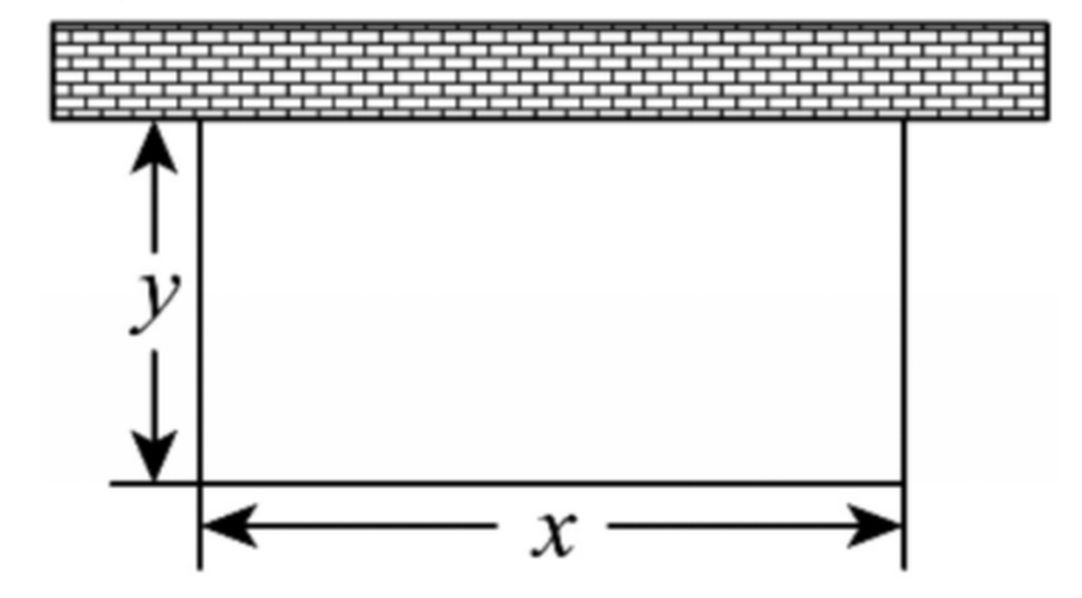
\includegraphics[width=0.42\textwidth]{figures/gao142_q20.png}
\end{center}

(1) 若菜园面积为 72 平方米，则 $x$、$y$ 为何值时，所用篱笆总长最小？

(2) 若 $x$、$y$ 满足 $x+y-xy+63=0$，则菜园面积最小为多少平方米？

\ifanswer
\solbegin
\step{(1) 由题意得，菜园的面积 $S=xy=72$，且 $x>0$，$y>0$，}
\step{所用篱笆总长 $L=x+2y$，}
\step{由基本不等式得 $x+2y\geqslant2\sqrt{x\cdot2y}=2\sqrt{2xy}=2\sqrt{2\times72}=24$，}
\step{当且仅当 $x=2y$ 时取等号，}
\step{联立 $\begin{cases}xy=72\\x=2y\end{cases}$，解得 $\begin{cases}x=12\\y=6\end{cases}$，}
\step{所以当 $x=12$，$y=6$ 时，所用篱笆总长最小；}
\step{(2) 由题意得 $x>0$，$y>0$，且满足 $x+y-xy+63=0$，即 $x+y=xy-63$，}
\step{由基本不等式得 $x+y\geqslant2\sqrt{xy}$，当且仅当 $x=y$ 时取等号，}
\step{所以 $xy-63\geqslant2\sqrt{xy}$. 令 $t=\sqrt{xy}(t>0)$，则 $xy=t^2$，}
\step{上述不等式可化为 $t^2-2t-63\geqslant0$，即 $(t-9)(t+7)\geqslant0$，}
\step{因为 $t>0$，所以 $t+7>0$，故 $t-9\geqslant0$，解得 $t\geqslant9$，所以 $\sqrt{xy}\geqslant9$，}
\step{即 $xy\geqslant81$，当且仅当 $x=y=9$ 时取等号，此时满足 $9+9-81+63=0$，}
\step{所以菜园面积最小为 81 平方米.}
\solend
\fi

\item 已知幂函数 $f(x)=(m^2-3m+3)x^m$ 的图象关于 $y$ 轴对称.

(1) 求实数 $m$ 的值；

(2) 在平面直角坐标系中作出函数 $y=\lvert f(x)-1\rvert$ 的图象；

(3) 已知点 $A(2a,y_1)$ 与点 $B(3-a,y_2)$ 都在幂函数 $y=x^2$ 的图象上. 若 $y_1<y_2$，求实数 $a$ 的取值范围.

\begin{center}
% 空白坐标网格取原卷 08 页截图去粉色水印、去色、LANCZOS 放大；题目配图，三版都出
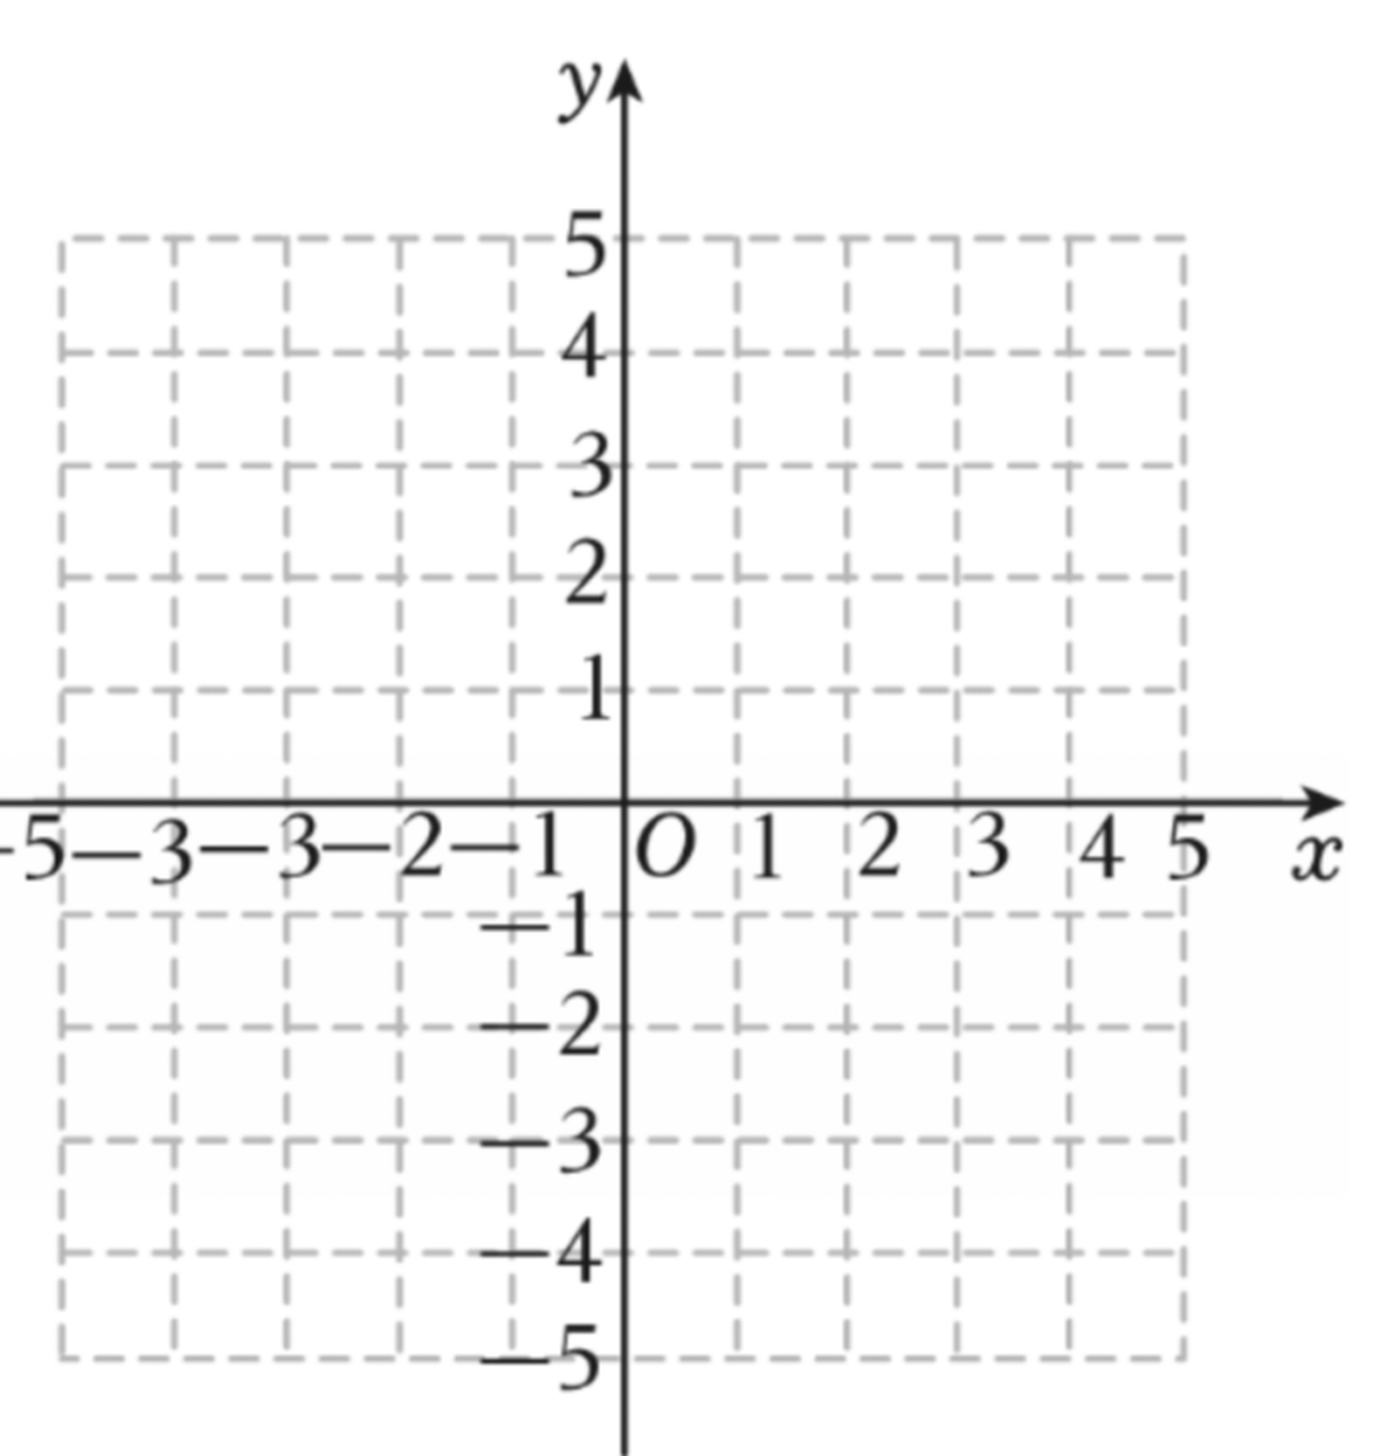
\includegraphics[width=0.52\textwidth]{figures/gao142_q21_grid.png}
\end{center}

\ifanswer
\solbegin
\step{(1) 由题意幂函数 $f(x)=(m^2-3m+3)x^m$，}
\step{故 $m^2-3m+3=1$，解得 $m=1$ 或 $m=2$，}
\step{又 $f(x)$ 图象关于 $y$ 轴对称，即 $f(x)$ 是偶函数，}
\step{当 $m=1$ 时，$f(x)=x$ 是奇函数，不满足条件，舍去；}
\step{当 $m=2$ 时，$f(x)=x^2$ 是偶函数，满足条件，故 $m=2$；}
\step{(2) 由 (1) 得，$\lvert f(x)-1\rvert=\lvert x^2-1\rvert$，}
\step{先画 $y=x^2-1$，开口向上的抛物线，顶点 $(0,-1)$，零点 $x=\pm1$，}
\step{再将 $x$ 轴下方的部分沿 $x$ 轴翻折到上方即为 $y=\lvert x^2-1\rvert$ 的图象，}
\step{图象如图所示.}
\par{\leftskip=0pt
\begin{center}
% 抛物线图象取原卷 09 页截图去粉色水印、去色、LANCZOS 放大；解析所附配图，仅答案版出
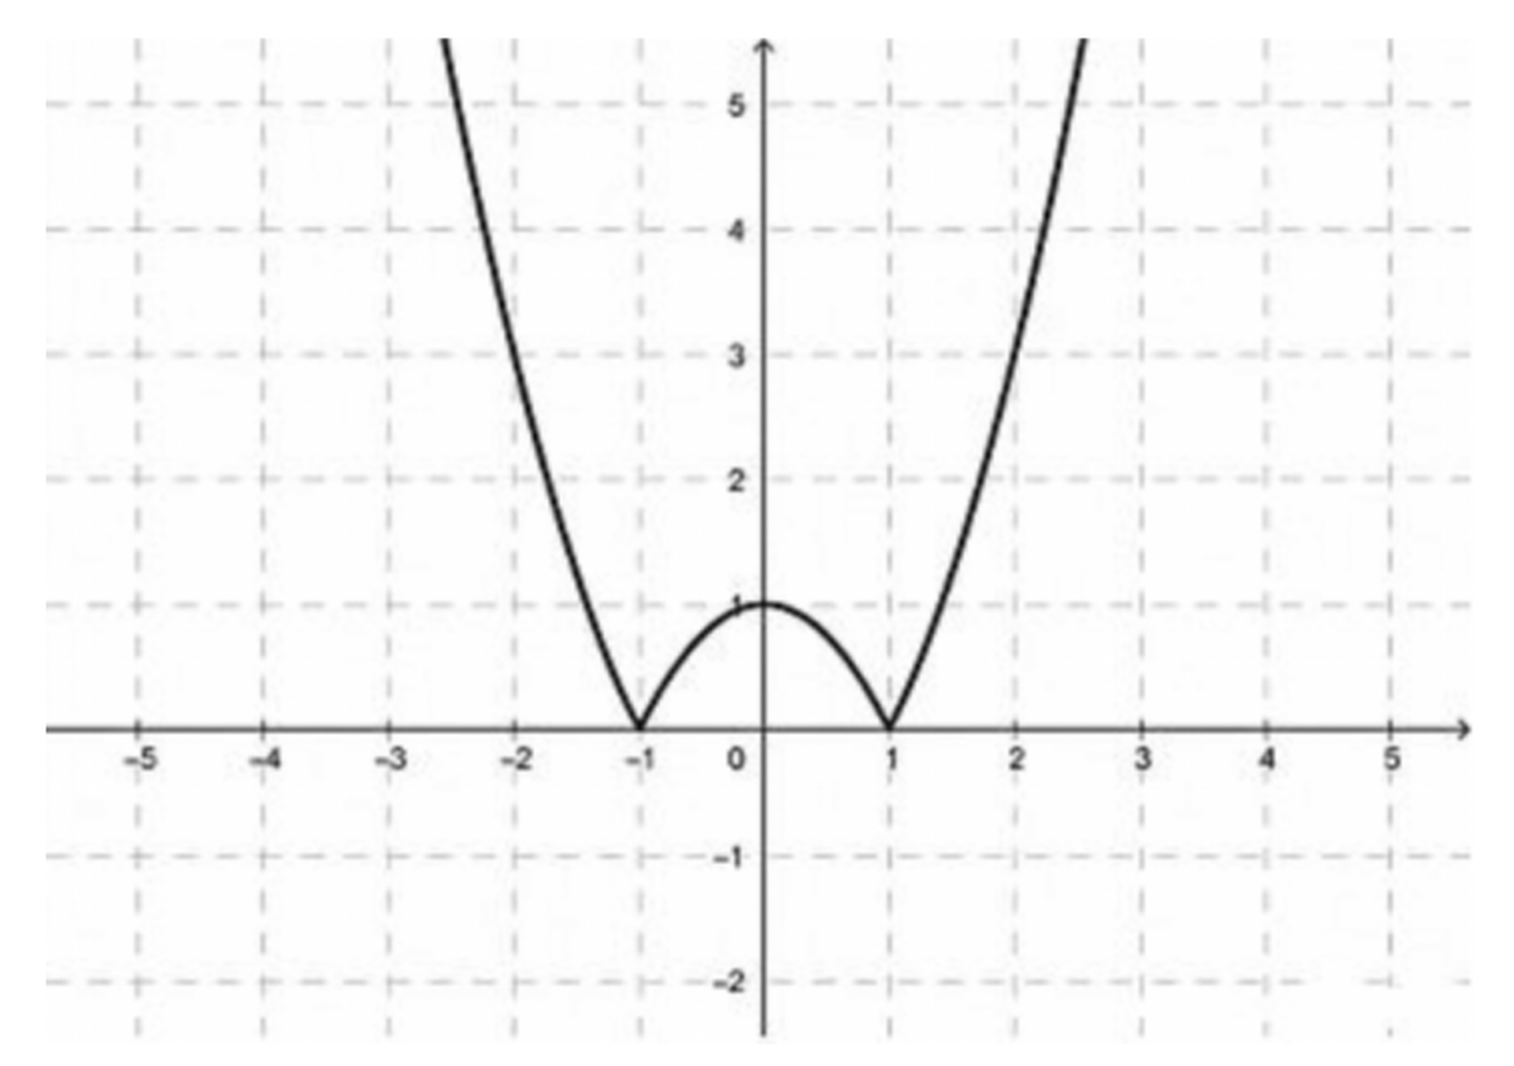
\includegraphics[width=0.55\textwidth]{figures/gao142_q21_para.png}
\end{center}}
\step{(3) 由题意得，$y_1=(2a)^2$，$y_2=(3-a)^2$，}
\step{$y_1<y_2$，即有 $(2a)^2<(3-a)^2$，化简整理得 $(a+3)(a-1)<0$，}
\step{解得实数 $a$ 的取值范围为 $(-3,1)$.}
\solend
\fi

\end{enumerate}

\end{document}
"
%
% ① 原始材料：微信公众号"魔都数学加油站"文章，连载"27学年高一142"，原文标题
% "27学年高一142——2026-2027年上海市群峰高级中学高一上期中"；
% 原文链接：https://mp.weixin.qq.com/s/cc7wnuP4Pk3OjNDV6ihB9A。
% 正文为 9 张 PNG 页（01、02、04、06、07、08、09 为 2560x3620；03、05 为 4762x6735，
% 同一篇各页分辨率不同，逐页按各自分辨率裁图核对），题目下印有【答案】或【解析】，为讲评版。
% 题目、解析均据原图转录；卷面粉红色水印"魔都数学加油站"及公众号页脚未录入。
% 全卷 4 幅插图：第 15 题四幅坐标函数图像选项（04 页，2x2 合并为一张）、
% 第 20 题矩形围栏示意图（07 页）、第 21 题 (2) 空白坐标网格（08 页）、
% 第 21 题抛物线图象（09 页，解析所附图）；均取原卷截图去粉色水印、LANCZOS 放大。
% 题目配图三版都出、解析配图仅答案版出。
%
% 卷首标题：原卷印作"2026-2027 年群峰高级中学高一上期中"（公众号标题中的"上海市"
% 卷面标题行没有，本稿照卷面），年份区间按全稿惯例排 en dash；原卷未印副标题，
% 本卷为期中卷、跨集合与常用逻辑用语／不等式／函数三章，按题目内容补出
% "集合与常用逻辑用语、不等式、函数"（头注说明，与同期中卷口径相同）。
%
% 题号体例：本卷共 19 题——一、填空题 3—12（10 题）、二、选择题 13—16（4 题）、
% 三、解答题 17—21（5 题）。三节分别 \setcounter{enumi}{2}／{12}／{16}。
% 原卷从第 3 题起、无第 1、2 题，本稿保留原题号。
%
% ② 与原卷的排版差异：
%   ① 原文从第 3 题起，本稿保留原题号；原卷未印副标题，本稿按"知识模块"口径补出；
%   ② 逐题答案口径：Q14 原卷把答案 D 印在题干括号内、且题目下无【解析】，本稿括号
%      留空 \mbox{（\quad）}、另提 \ans{D}；Q13／Q15／Q16 答案在【解析】末句"故选 …"
%      （分别为 C／C／A），题干括号留空、不另提 \ans{}；其余各题（Q3—Q12、
%      Q17—Q21）题目下印【解析】、答案融在解析中，不另提 \ans{}；全卷仅 Q14 一处 \ans{}；
%      答案版【答案】/【解析】标记数 = 19（1 个 \ans + 18 个 \solbegin）= 全卷题数；
%   ③ 原卷填空横线按全稿惯例排 \blankline[4.4em]；选择题括号排 \mbox{（\quad）}、
%      每个选项段前按惯例加 \keepwithprev（Q15 四幅图那一枚放在 \begin{center} 之前）；
%      解答题不留作答区、不加 \anspace（原卷为讲评版，与 129／131／132／133／136／140 同）；
%   ④ 原卷数集斜体 $R$（Q5、Q7、Q19、Q21 解析等）按全稿惯例统一改 \R；空集记号
%      \varnothing；绝对值排 \lvert…\rvert，集合描述竖线排 \mid；不等号按全稿惯例
%      排 \leqslant／\geqslant；
%   ⑤ 4 幅插图：Q15 四幅坐标函数图象选项合并裁为一张 \includegraphics（题前
%      \needvspace{9cm}）；Q15 是"二、选择题"节内带大图块的第 3 题（Q13、Q14 在前
%      且无图），另在 \bigsec{二、选择题} 之前加 \needvspace{11cm} 连节标题一起量
%      ——守卫必须放在 \bigsec 之前，放标题之后会让"二、选择题"孤立在页末
%      （B 类，照 高一26／40／59／136／140 成例）；Q20 围栏图与 Q21 网格图置于题干
%      之后（三版都出），Q21 抛物线图置于答案版解析 (2) 与 (3) 之间（仅答案版出）；
%   ⑥ 子题标号按原卷排半角 (1)(2)(3)（与 140／141 同期中卷口径相同）；括注全角／
%      半角逐处照录：Q3"（用含有 m 的代数式表示）"、Q6"（舍）"、Q10"（万元）"、
%      Q18"（请务必书写必要的计算步骤）"、Q20"（墙足够长）"印全角；Q15
%      "$y=a^x(a>0 且 a\neq1)$"、Q10"$y=x^a(a 为常数)$"、Q20"$t=\sqrt{xy}(t>0)$"
%      等数学式内括注印半角；数学式内 CJK 用 \text{…}（否则 FONTCHK 报缺字）；
%   ⑦ 数学式内半角逗号照录（如 Q6"$ax-1=0,a\in\R$"、Q9"$b=2+\sqrt2,a=\sqrt2+1$"、
%      Q16 区间 "$[-1,3]$"、Q21"$y_1<y_2$，即 $(2a)^2<(3-a)^2$" 等）；原卷行末
%      西文句点照录（Q7"(-3,5)."、Q10"125（万元）."、Q19 题干句点、Q20 题干
%      "矩形菜园."与"宽为 y 米."、Q21 题干"对称." 等）；行中全角逗号、分号照录；
%   ⑧ 题干中的中文弯引号：本卷题干与解析通篇未出现中文弯引号，故无此项；
%      圈数字 ①②③ 亦未出现（子题用 (1)(2)(3)）；
%   ⑨ 原卷"图像／图象"两种写法混用，逐处放大核对并照录：Q4 题干与解析作"图象"、
%      Q7 解析作"图象"、Q8 题干作"图像"而解析作"图象"、Q15 题干与解析通篇作
%      "图像"、Q21 题干与解析通篇作"图象"；
%   ⑩ 原卷无红色加粗标签（【解析】均黑色印刷；逐页扫描深红像素为 0），故本卷未用
%      \stepm；黑色常规分步标签（"A 中""C 中""D 中""(1)(2)(3)" 等）按普通 \step
%      行内文字照录；
%   ⑪ 跨页续印按题合并，明细见 ⑥。
%
% ③ 行数复核：一条 \step = 原卷解析的一个印刷行，cases 块作一个印刷行计。逐题数 \step
%   条数，合计 98 条（Q3：1；Q4：2；Q5：3；Q6：4；Q7：5；Q8：2；Q9：4；Q10：3；
%   Q11：4；Q12：3；Q13：5；Q14：0；Q15：10；Q16：4；Q17：10；Q18：3；
%   Q19：10；Q20：13；Q21：12），与原卷印刷行逐题相等。Q14 只把答案印在题干括号、
%   无【解析】，提 \ans{D}、不计入 \step 账；答案版标记数 = 19（1 个 \ans + 18 个
%   \solbegin）= 全卷题数。
%
% ④ 判别式字形：全卷判别式共 3 处——第 7 题【解析】"即判别式△<0"、
%   "即△=(a-1)^2-4×1×4<0" 两处原卷印扁等边三角 $\triangle$，
%   第 11 题【解析】cases 块"△=4a^2-4(a+6)≥0" 一处原卷印等腰偏高的高三角 $\Delta$；
%   逐处放大核对，两形不同、全卷混用，本稿逐处照录不统一（参照 高一141 头注④口径）。
%   子集符号：全卷共 3 处——第 6 题题干"若 B⊆A"、第 6 题【解析】"因为 B⊆A"、
%   第 17 题【解析】(2)"所以 A⊆B"，逐处放大核对，原卷三处均印带下划线的
%   $\subseteq$（不是单线 $\subset$），本稿一律照录 \subseteq；全卷未出现 \subset。
%
% ⑤ 原卷存疑照录（均照录未改，正文对应处另有 % 注）：
%   第 14 题题干括号内原卷印答案 D（非留空），且题目下无【解析】，按"答案印括号且
%      无解析"口径括号留空、另提 \ans{D}；
%   第 15 题【解析】"C 中，由指数函数 … 图像递减得 a>1" 中"递减"与"a>1"
%      自相矛盾（递减应得 0<a<1，疑为"递增"之误），照录；
%   第 16 题选项 B 作 $(-\infty,3]\cup[3,+\infty)$，两端区间并起即全体实数、
%      与正确答案 $[-1,3]$ 不成干扰项（疑为 $(-\infty,-1]\cup[3,+\infty)$ 之误），照录；
%   第 21 题 (2) 空白坐标网格的 x 轴刻度原卷印作"-5 -3 -3 -2 -1 0 1 2 3 4 5"
%      （"-3"重复，疑为"-4"之误），系插图中的印刷内容，取原卷截图照录、不改图。
%
% ⑥ 跨页续印说明：Q7 题干与解析首行在 01 页、解析续至 02 页；Q11 题干与解析
%   4 行在 03 页；Q13 解析前 4 行在 03 页、末句"故选 C."续至 04 页；Q15 题干与
%   四幅图在 04 页、解析前 8 行在 04 页、末 2 行续至 05 页；Q17 解析前 7 行在
%   05 页、后 3 行续至 06 页；Q19 解析前 5 行在 06 页、后 5 行续至 07 页；
%   Q20 解析前 9 行在 07 页、后 4 行续至 08 页；Q21 解析 (1)(2) 9 行在 08 页、
%   抛物线图与 (3) 3 行续至 09 页；本稿按题连排，不丢行。三版切页审计结论见
%   编译自验回报（切页守卫见 ②⑤）。
%
\documentclass[a4paper,11pt]{article}
\usepackage{common}

\begin{document}

\examtitlest[3]{2026--2027 年群峰高级中学高一上期中}{集合与常用逻辑用语、不等式、函数}

\bigsec{一、填空题}

\begin{enumerate}
\setcounter{enumi}{2}

\item 已知 $\log_2 3=m$，则 $\log_3 6=$\blankline[4.4em]（用含有 $m$ 的代数式表示）.

\ifanswer
\solbegin
\step{$\log_3 6=\dfrac{\log_2 6}{\log_2 3}=\dfrac{\log_2 2+\log_2 3}{\log_2 3}=\dfrac{1+m}{m}=\dfrac1m+1$.}
\solend
\fi

\item 若指数函数 $y=a^x$ 的图象经过点 $(3,27)$，则 $a$ 的值为\blankline[4.4em].

\ifanswer
\solbegin
\step{因为指数函数 $y=a^x$ 的图象经过点 $(3,27)$，}
\step{所以 $a^3=27=3^3$，所以 $a=3$.}
\solend
\fi

\item 不等式 $(2x+1)^{\frac13}<(3-x)^{\frac13}$ 的解集为\blankline[4.4em].

\ifanswer
\solbegin
\step{因为幂函数 $f(t)=t^{\frac13}$ 在 $\R$ 上严格增，}
\step{所以原不等式等价于 $2x+1<3-x$，解得 $x<\dfrac23$，}
\step{因此原不等式的解集为 $\left(-\infty,\dfrac23\right)$.}
\solend
\fi

\item 设集合 $A=\{1,-2\}$，$B=\{x\mid ax-1=0,a\in\R\}$，若 $B\subseteq A$，则 $a$ 的值为\blankline[4.4em].% 子集符号原卷印带下划线 $\subseteq$，照录

\ifanswer
\solbegin
\step{因为 $B\subseteq A$，所以 $B=\varnothing$ 或 $\{-2\}$ 或 $\{1\}$ 或 $\{1,-2\}$（舍），}% 子集符号原卷印带下划线 $\subseteq$，照录
\step{若 $B=\varnothing$，则 $a=0$；若 $B=\{1\}$，则 $a=1$；}
\step{若 $B=\{-2\}$，则 $-2a=1$，解得 $a=-\dfrac12$；}
\step{综上，$a=0$ 或 $1$ 或 $-\dfrac12$.}
\solend
\fi

\item 不等式 $x^2+(a-1)x+4>0$ 在 $\R$ 上恒成立，则实数 $a$ 的取值范围是\blankline[4.4em].

\ifanswer
\solbegin
\step{不等式 $x^2+(a-1)x+4>0$，对应的二次函数为 $y=x^2+(a-1)x+4$，}
\step{因此函数图象开口向上，要使不等式对任意实数 $x$ 恒成立，}
\step{需二次函数图象与 $x$ 轴无交点，即判别式 $\triangle<0$，}% 判别式原卷印扁等边三角 $\triangle$，照录
\step{即 $\triangle=(a-1)^2-4\times1\times4<0$，整理得 $a^2-2a-15<0$，}% 判别式原卷印扁等边三角 $\triangle$，照录
\step{解得 $-3<a<5$，故实数 $a$ 的取值范围是 $(-3,5)$.}
\solend
\fi

\item 函数 $f(x)=(5x-3)^a$ 的图像恒过点\blankline[4.4em].% 题干作"图像"、解析作"图象"，原卷混用，逐处照录

\ifanswer
\solbegin
\step{令 $5x-3=1$ 得 $x=\dfrac45$，此时 $f\left(\dfrac45\right)=\left(5\times\dfrac45-3\right)^a=1$，}
\step{所以 $f(x)$ 的图象恒过 $\left(\dfrac45,1\right)$.}
\solend
\fi

\item 若 $a>0$，$b>0$ 且 $\dfrac1a+\dfrac2b=1$，则 $a+b$ 的最小值为\blankline[4.4em].

\ifanswer
\solbegin
\step{因为 $a>0$，$b>0$，$\dfrac1a+\dfrac2b=1$，}
\step{所以 $a+b=(a+b)\left(\dfrac1a+\dfrac2b\right)=1+\dfrac{2a}{b}+\dfrac{b}{a}+2\geqslant3+2\sqrt{\dfrac{2a}{b}\cdot\dfrac{b}{a}}=3+2\sqrt2$，}
\step{当且仅当 $\dfrac{2a}{b}=\dfrac{b}{a}$，即 $b=2+\sqrt2,a=\sqrt2+1$ 时取等号，}
\step{故 $a+b$ 的最小值为 $3+2\sqrt2$.}
\solend
\fi

\item 某药厂研制出一种新型药剂，投放市场后其广告投入 $x$（万元）与药品利润 $y$（万元）存在的关系为 $y=x^a(a\text{ 为常数})$，其中 $x$ 不超过 5 万元. 已知去年投入广告费用为 3 万元时，药品利润为 27 万元，若今年投入广告费用 5 万元，预计今年药品利润为\blankline[4.4em]万元.

\ifanswer
\solbegin
\step{由已知投入广告费用为 3 万元时，药品利润为 27 万元，}
\step{代入 $y=x^a$ 中，即 $3^a=27$，解得 $a=3$，故函数关系式为 $y=x^3$，}
\step{所以当 $x=5$ 时，$y=125$（万元）.}
\solend
\fi

\item 已知方程 $x^2+2ax+a+6=0$ 的两根分别是 $x_1$ 和 $x_2$，且满足 $\dfrac1{x_1}+\dfrac1{x_2}<0$，则实数 $a$ 的取值范围是\blankline[4.4em].

\ifanswer
\solbegin
\step{由于方程 $x^2+2ax+a+6=0$ 的两根分别是 $x_1$ 和 $x_2$，}
\step{则 $\begin{cases}\Delta=4a^2-4(a+6)\geqslant0\\x_1+x_2=-2a\\x_1x_2=a+6\end{cases}$，解得 $a\geqslant3$ 或 $a\leqslant-2$.}% 判别式原卷印等腰偏高的高三角 $\Delta$，照录（与第 7 题扁等边 $\triangle$ 两形混用）
\step{又 $\dfrac1{x_1}+\dfrac1{x_2}<0$，即 $\dfrac{x_1+x_2}{x_1\cdot x_2}<0$，故 $\dfrac{-2a}{a+6}<0$，解得 $a<-6$ 或 $a>0$.}
\step{综上，$a$ 的取值范围是 $(-\infty,-6)\cup[3,+\infty)$.}
\solend
\fi

\item 已知 $b>a>1$，若 $\log_a b-\log_b a=\dfrac32$，$a^b=b^a$，则 $a-b=$\blankline[4.4em].

\ifanswer
\solbegin
\step{因为 $b>a>1$，所以 $\log_a b>1$，}
\step{由 $\log_a b-\log_b a=\log_a b-\dfrac{1}{\log_a b}=\dfrac32$，解得 $\log_a b=2$ 即 $b=a^2$，}
\step{因为 $a^b=b^a=a^{2a}$，所以 $b=2a=a^2$，所以 $a=2$，$b=4$，则 $a-b=-2$.}
\solend
\fi

\end{enumerate}

% 第 15 题四幅图是"二、选择题"节内的大图块；守卫须放在 \bigsec 之前连节标题一起量
\needvspace{11cm}
\bigsec{二、选择题}

\begin{enumerate}
\setcounter{enumi}{12}

\item 若 $a>b$，$c<0$，则下列不等式正确的是\mbox{（\quad）}

\keepwithprev
A. $ab>bc$\qquad B. $a+c<b+c$\qquad C. $ac^2>bc^2$\qquad D. $\dfrac ac>\dfrac bc$

\ifanswer
\solbegin
\step{因为 $a>b$，$c<0$，取 $b=0$，则 $ab=bc=0$，故 $A$ 错误；}
\step{由于 $a>b$，所以 $a+c>b+c$，故 $B$ 错误；}
\step{由 $c<0$ 得 $c^2>0$，所以 $ac^2>bc^2$，故 $C$ 正确；}
\step{由于 $a>b$ 且 $c<0$，所以 $\dfrac ac<\dfrac bc$，故 $D$ 错误.}
\step{故选 $C$.}
\solend
\fi

\item 若 $x>0$，$y>0$，则下列各式中，恒成立的是\mbox{（\quad）}% 原卷题干括号内印答案 D、且题目下无【解析】，本稿括号留空、另提 \ans{D}

\keepwithprev
A. $\lg x+\lg y=\lg(x+y)$\qquad B. $\lg x^2=(\lg x)^2$

C. $\dfrac{\lg x}{\lg y}=\lg(x-y)$\qquad D. $\lg x^{\frac1n}=\dfrac{\lg x}{n}$

\ifanswer
\ans{$D$}
\fi

% 第 15 题四幅坐标函数图象选项是一整块，守卫放在 \item 之前
\needvspace{9cm}
\item 在同一平面直角坐标系中，指数函数 $y=a^x(a>0\text{ 且 }a\neq1)$ 和一次函数 $y=a(x+1)$ 的图像关系可能是\mbox{（\quad）}

\keepwithprev
\begin{center}
% 四幅坐标函数图象选项取原卷 04 页截图去粉色水印、去色，按原卷 2x2 排布合并为一张
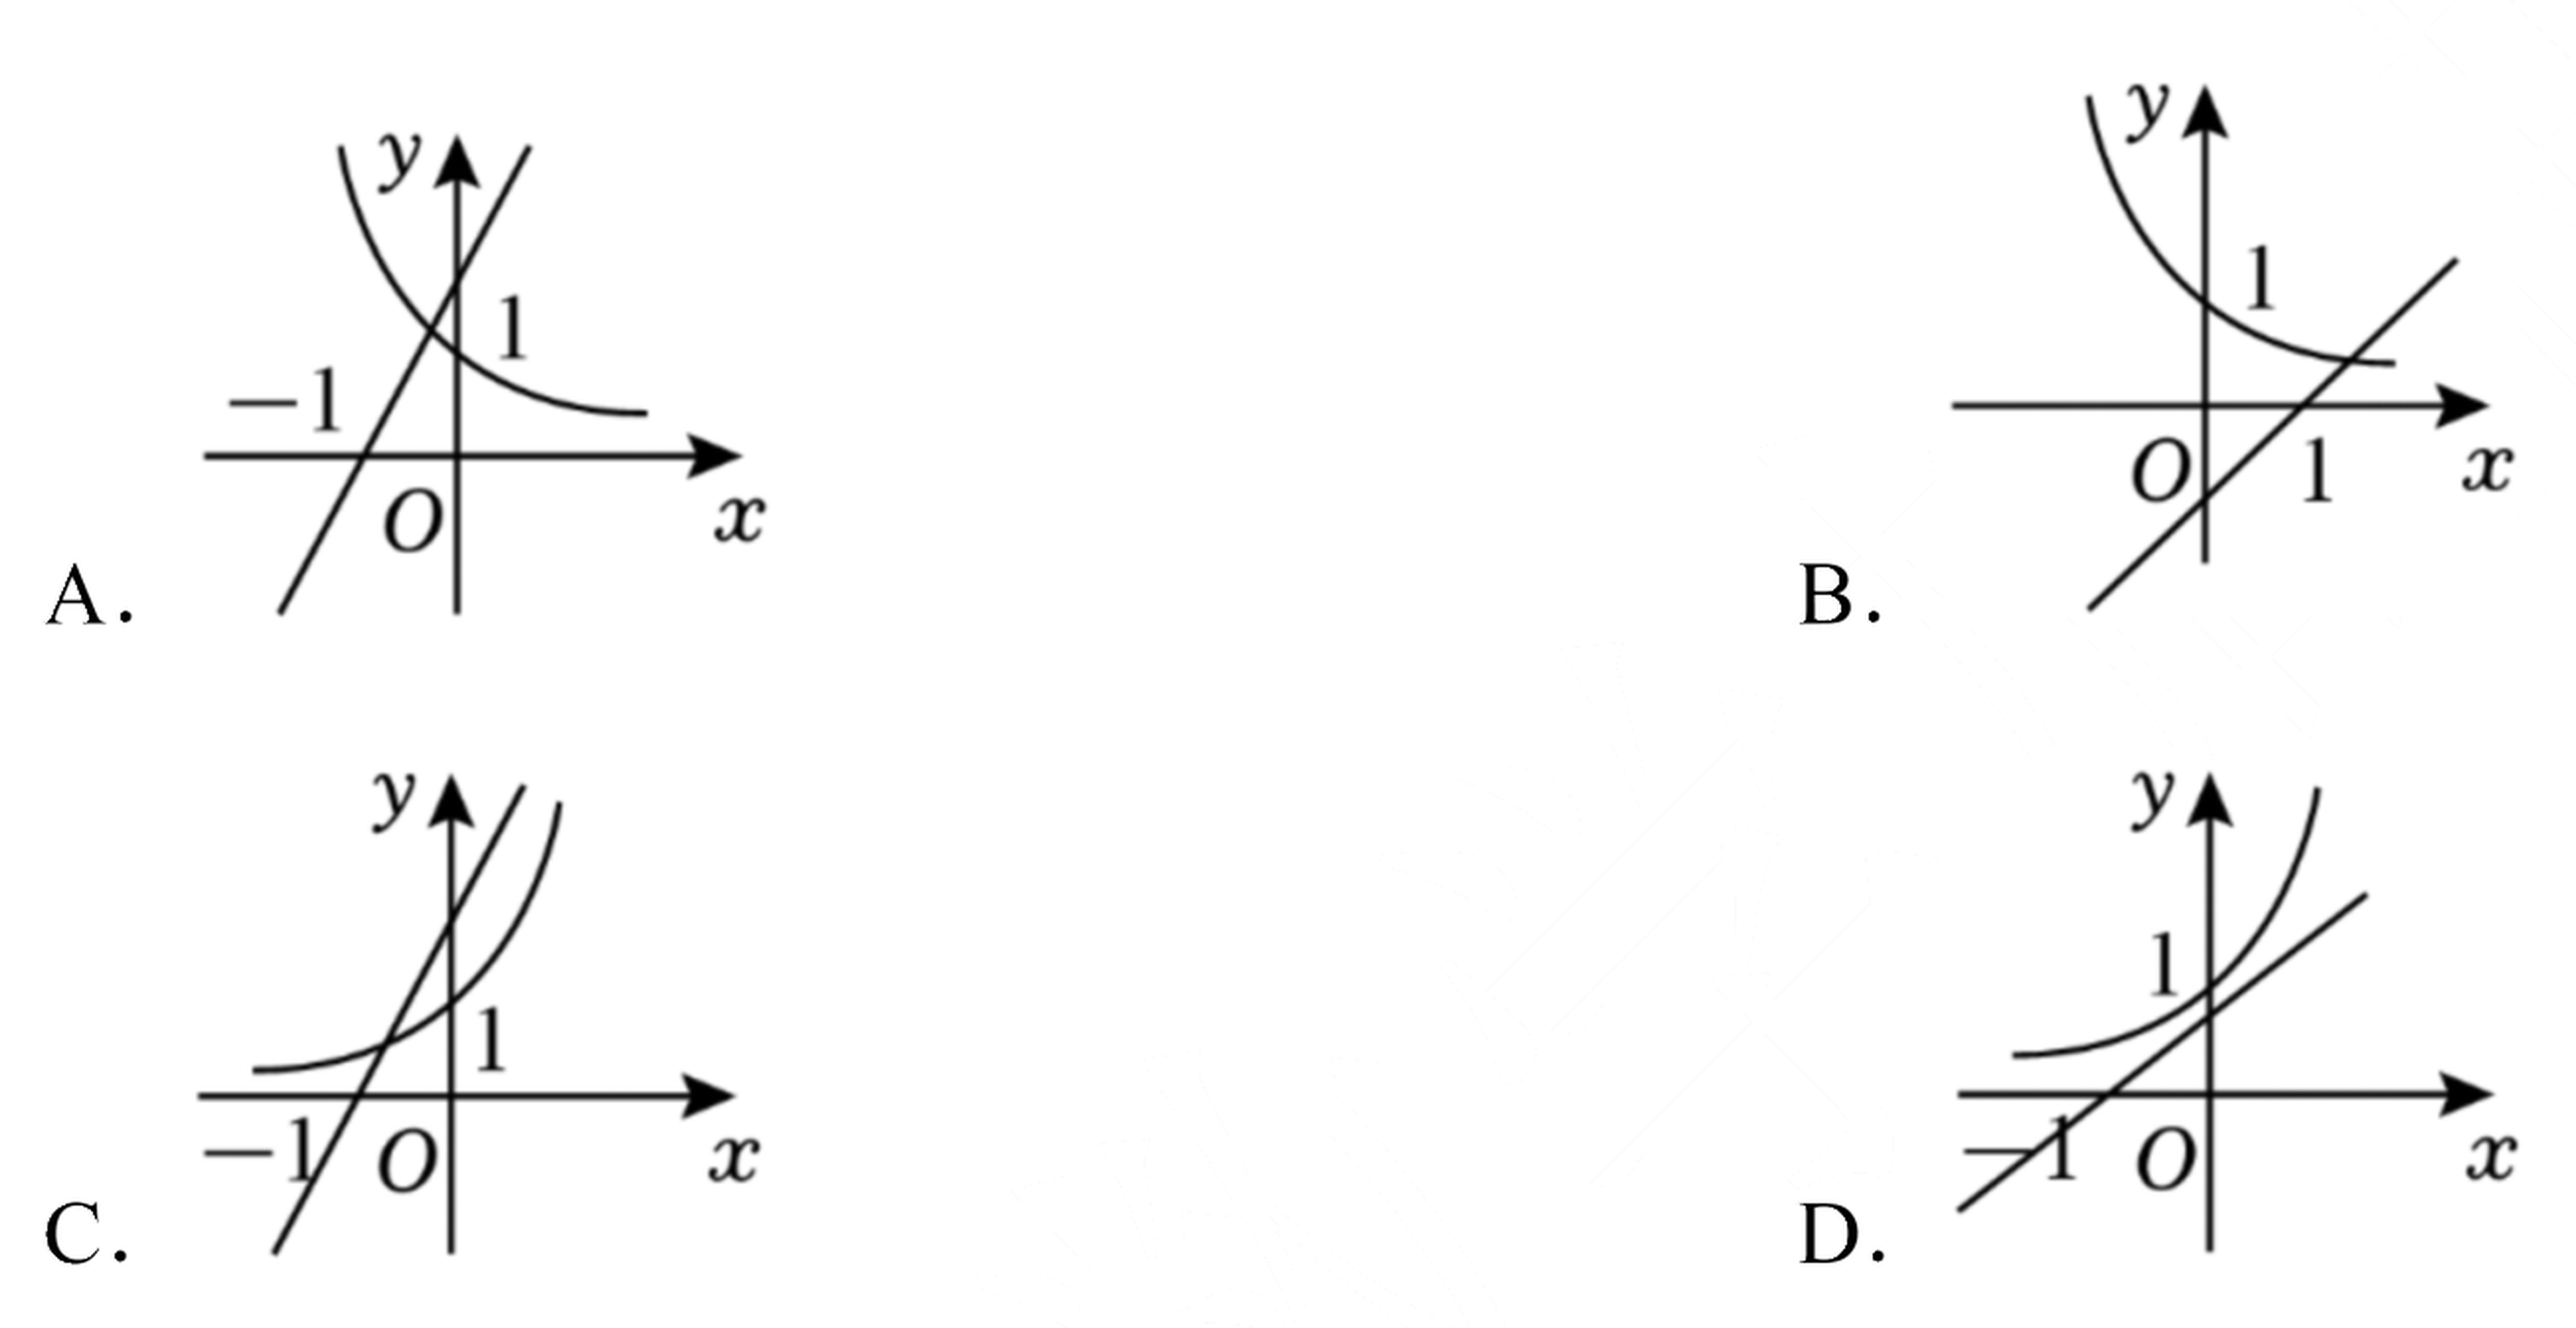
\includegraphics[width=0.80\textwidth]{figures/gao142_q15.png}
\end{center}

\ifanswer
\solbegin
\step{$A$ 中，由指数函数 $y=a^x(a>0\text{ 且 }a\neq1)$ 图像递减得 $0<a<1$，}
\step{而一次函数 $y=a(x+1)$ 的图像与 $y$ 轴交点纵坐标为 $a>1$，二者矛盾，}
\step{所以 $A$ 错；}
\step{由一次函数 $y=a(x+1)$ 的图像与 $x$ 轴交点横坐标为 $-1$，排除 $B$；}
\step{$C$ 中，由指数函数 $y=a^x(a>0\text{ 且 }a\neq1)$ 图像递减得 $a>1$，}% 原卷"递减得 a>1"自相矛盾（递减应得 0<a<1），照录
\step{而一次函数 $y=a(x+1)$ 的图像与 $y$ 轴交点纵坐标为 $a>1$，二者 $a$ 值吻合，}
\step{所以 $C$ 对；}
\step{$D$ 中，由一次函数 $y=a(x+1)$ 的图像得 $a=1$，与 $a>0$ 且 $a\neq1$ 矛盾，}
\step{所以 $D$ 错.}
\step{故选 $C$.}
\solend
\fi

\item 不等式 $\lvert x+1\rvert+\lvert 2-x\rvert\geqslant a^2-2a$ 恒成立，则 $a$ 的取值范围是\mbox{（\quad）}

\keepwithprev
A. $[-1,3]$\qquad B. $(-\infty,3]\cup[3,+\infty)$\qquad C. $(-\infty,3)$\qquad D. $(3,+\infty)$

\ifanswer
\solbegin
\step{因为 $\lvert x+1\rvert+\lvert 2-x\rvert\geqslant\lvert(x+1)+(2-x)\rvert=3$，}
\step{所以 $\lvert x+1\rvert+\lvert 2-x\rvert$ 的最小值为 3，}
\step{因为 $\lvert x+1\rvert+\lvert 2-x\rvert\geqslant a^2-2a$ 恒成立，所以只需 $a^2-2a\leqslant3$，所以 $-1\leqslant a\leqslant3$，}
\step{所以 $a$ 的取值范围为 $[-1,3]$. 故选 $A$.}
\solend
\fi

\end{enumerate}

\bigsec{三、解答题}

\begin{enumerate}
\setcounter{enumi}{16}

\item 已知集合 $A=\left\{x\mid\dfrac{x-3}{x-1}\leqslant0\right\}$，$B=\{x\mid\lvert x-1\rvert<a\}$.

(1) 若 $a=1$，求 $A\cap B$；

(2) 若 $x\in A$ 是 $x\in B$ 的充分条件，求 $a$ 的取值范围.

\ifanswer
\solbegin
\step{(1) 不等式 $\dfrac{x-3}{x-1}\leqslant0$，等价于 $(x-3)(x-1)\leqslant0$ 且 $x-1\neq0$，解得 $1<x\leqslant3$，}
\step{所以 $A=\{x\mid 1<x\leqslant3\}$，}
\step{当 $a=1$ 时，不等式 $\lvert x-1\rvert<a$ 可化为 $\lvert x-1\rvert<1$，所以 $-1<x-1<1$，}
\step{故 $0<x<2$，所以 $B=\{x\mid 0<x<2\}$，}
\step{所以 $A\cap B=\{x\mid 1<x<2\}$；}
\step{(2) 因为 $x\in A$ 是 $x\in B$ 的充分条件，所以 $A\subseteq B$，}% 子集符号原卷印带下划线 $\subseteq$，照录
\step{因为 $A=\{x\mid 1<x\leqslant3\}\neq\varnothing$，所以 $B\neq\varnothing$，故 $a>0$，}
\step{由不等式 $\lvert x-1\rvert<a$，解得 $1-a<x<1+a$，}
\step{所以 $B=\{x\mid 1-a<x<1+a\}$，所以 $\begin{cases}1-a\leqslant1\\1+a>3\end{cases}$，解得 $a>2$，}
\step{所以 $a$ 的取值范围为 $(2,+\infty)$.}
\solend
\fi

\item 计算下列式子的值（请务必书写必要的计算步骤）

(1) $27^{\frac13}+\left(\dfrac76\right)^0+\sqrt{(3-\pi)^2}$；

(2) $\lg25+\lg4+7^{\log_7 2}-\log_2 3\times\log_3 4+\log_3 9$.

\ifanswer
\solbegin
\step{(1) $27^{\frac13}+\left(\dfrac76\right)^0+\sqrt{(3-\pi)^2}=3^{3\times\frac13}+1+\lvert 3-\pi\rvert=3+1+\pi-3=\pi+1$；}
\step{(2) 原式 $=\lg(25\times4)+2-\dfrac{\lg3}{\lg2}\times\dfrac{\lg4}{\lg3}+2=\lg100+2-\dfrac{2\lg2}{\lg2}+2$}
\step{$=2+2-2+2=4$.}
\solend
\fi

\item 已知关于 $x$ 的不等式 $mx^2-(3m^2-m+2)x+6m-2\geqslant0$.

(1) 当 $m=2$ 时，求关于 $x$ 的不等式的解集；

(2) 当 $m>0$ 时，求关于 $x$ 的不等式的解集.

\ifanswer
\solbegin
\step{(1) $m=2$ 时，不等式为 $x^2-6x+5\geqslant0$，即 $(x-1)(x-5)\geqslant0$，}
\step{解得 $x\leqslant1$ 或 $x\geqslant5$，所以不等式的解集是 $\{x\mid x\leqslant1$ 或 $x\geqslant5\}$.}
\step{(2) $m>0$ 时，不等式可化为 $(mx-2)[x-(3m-1)]\geqslant0$，}
\step{即 $\left(x-\dfrac2m\right)[x-(3m-1)]\geqslant0$，}
\step{若 $m=1$，则不等式为 $(x-2)^2\geqslant0$，解得 $x\in\R$；}
\step{若 $0<m<1$，则 $\dfrac2m>3m-1$，解不等式得 $x\geqslant\dfrac2m$ 或 $x\leqslant3m-1$；}
\step{若 $m>1$，则 $\dfrac2m<3m-1$，解不等式得 $x\geqslant3m-1$ 或 $x\leqslant\dfrac2m$；}
\step{综上，$0<m<1$ 时，不等式的解集是 $\{x\mid x\leqslant3m-1$ 或 $x\geqslant\dfrac2m\}$；}
\step{$m=1$ 时，不等式的解集为 $\R$；}
\step{$m>1$ 时，不等式的解集是 $\{x\mid x\leqslant\dfrac2m$ 或 $x\geqslant3m-1\}$.}
\solend
\fi

\item 如图，某人计划用篱笆围成一个一边靠墙（墙足够长）的矩形菜园. 设菜园的长为 $x$ 米，宽为 $y$ 米.

\begin{center}
% 矩形围栏示意图取原卷 07 页截图去粉色水印、去色、LANCZOS 放大；题目配图，三版都出
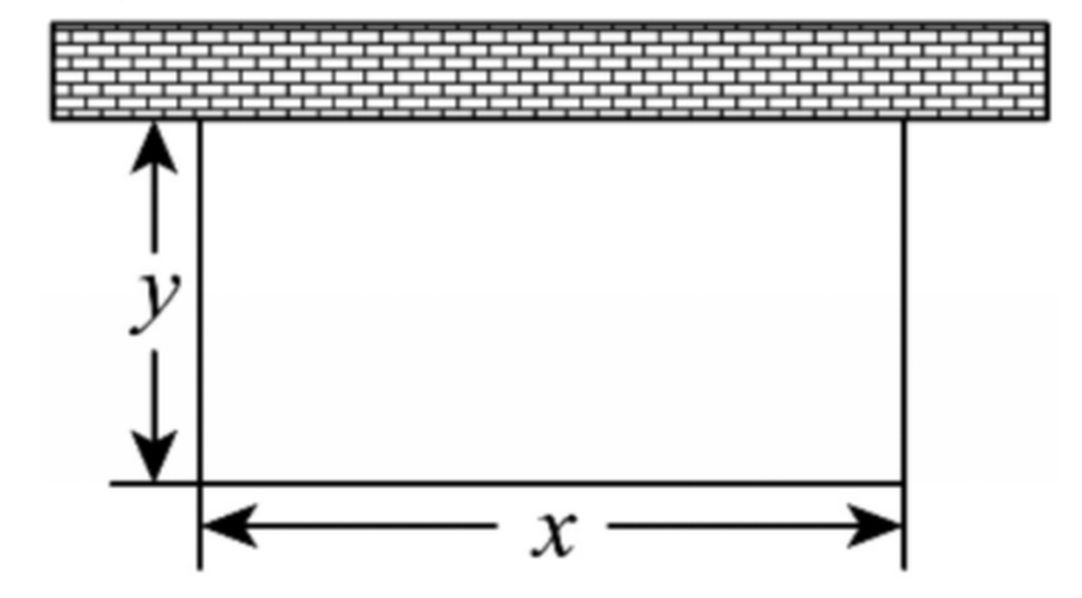
\includegraphics[width=0.42\textwidth]{figures/gao142_q20.png}
\end{center}

(1) 若菜园面积为 72 平方米，则 $x$、$y$ 为何值时，所用篱笆总长最小？

(2) 若 $x$、$y$ 满足 $x+y-xy+63=0$，则菜园面积最小为多少平方米？

\ifanswer
\solbegin
\step{(1) 由题意得，菜园的面积 $S=xy=72$，且 $x>0$，$y>0$，}
\step{所用篱笆总长 $L=x+2y$，}
\step{由基本不等式得 $x+2y\geqslant2\sqrt{x\cdot2y}=2\sqrt{2xy}=2\sqrt{2\times72}=24$，}
\step{当且仅当 $x=2y$ 时取等号，}
\step{联立 $\begin{cases}xy=72\\x=2y\end{cases}$，解得 $\begin{cases}x=12\\y=6\end{cases}$，}
\step{所以当 $x=12$，$y=6$ 时，所用篱笆总长最小；}
\step{(2) 由题意得 $x>0$，$y>0$，且满足 $x+y-xy+63=0$，即 $x+y=xy-63$，}
\step{由基本不等式得 $x+y\geqslant2\sqrt{xy}$，当且仅当 $x=y$ 时取等号，}
\step{所以 $xy-63\geqslant2\sqrt{xy}$. 令 $t=\sqrt{xy}(t>0)$，则 $xy=t^2$，}
\step{上述不等式可化为 $t^2-2t-63\geqslant0$，即 $(t-9)(t+7)\geqslant0$，}
\step{因为 $t>0$，所以 $t+7>0$，故 $t-9\geqslant0$，解得 $t\geqslant9$，所以 $\sqrt{xy}\geqslant9$，}
\step{即 $xy\geqslant81$，当且仅当 $x=y=9$ 时取等号，此时满足 $9+9-81+63=0$，}
\step{所以菜园面积最小为 81 平方米.}
\solend
\fi

\item 已知幂函数 $f(x)=(m^2-3m+3)x^m$ 的图象关于 $y$ 轴对称.

(1) 求实数 $m$ 的值；

(2) 在平面直角坐标系中作出函数 $y=\lvert f(x)-1\rvert$ 的图象；

(3) 已知点 $A(2a,y_1)$ 与点 $B(3-a,y_2)$ 都在幂函数 $y=x^2$ 的图象上. 若 $y_1<y_2$，求实数 $a$ 的取值范围.

\begin{center}
% 空白坐标网格取原卷 08 页截图去粉色水印、去色、LANCZOS 放大；题目配图，三版都出
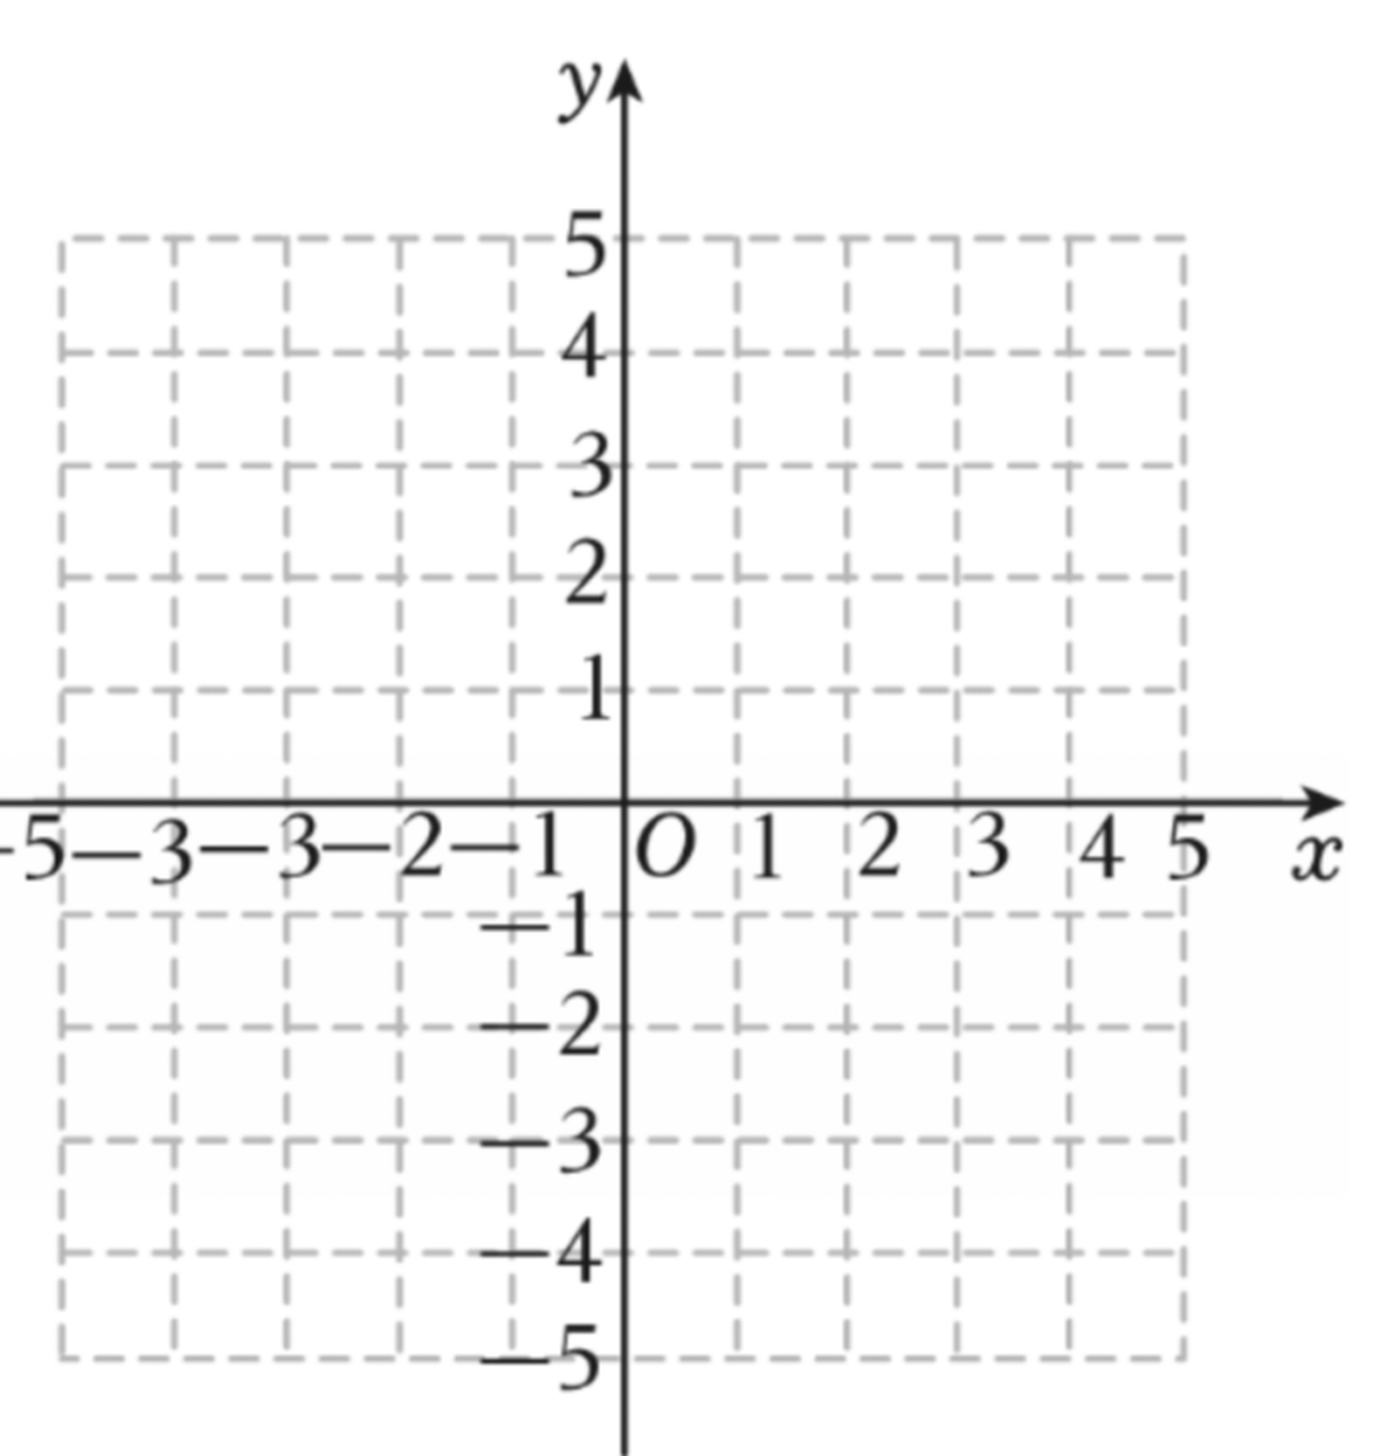
\includegraphics[width=0.52\textwidth]{figures/gao142_q21_grid.png}
\end{center}

\ifanswer
\solbegin
\step{(1) 由题意幂函数 $f(x)=(m^2-3m+3)x^m$，}
\step{故 $m^2-3m+3=1$，解得 $m=1$ 或 $m=2$，}
\step{又 $f(x)$ 图象关于 $y$ 轴对称，即 $f(x)$ 是偶函数，}
\step{当 $m=1$ 时，$f(x)=x$ 是奇函数，不满足条件，舍去；}
\step{当 $m=2$ 时，$f(x)=x^2$ 是偶函数，满足条件，故 $m=2$；}
\step{(2) 由 (1) 得，$\lvert f(x)-1\rvert=\lvert x^2-1\rvert$，}
\step{先画 $y=x^2-1$，开口向上的抛物线，顶点 $(0,-1)$，零点 $x=\pm1$，}
\step{再将 $x$ 轴下方的部分沿 $x$ 轴翻折到上方即为 $y=\lvert x^2-1\rvert$ 的图象，}
\step{图象如图所示.}
\par{\leftskip=0pt
\begin{center}
% 抛物线图象取原卷 09 页截图去粉色水印、去色、LANCZOS 放大；解析所附配图，仅答案版出
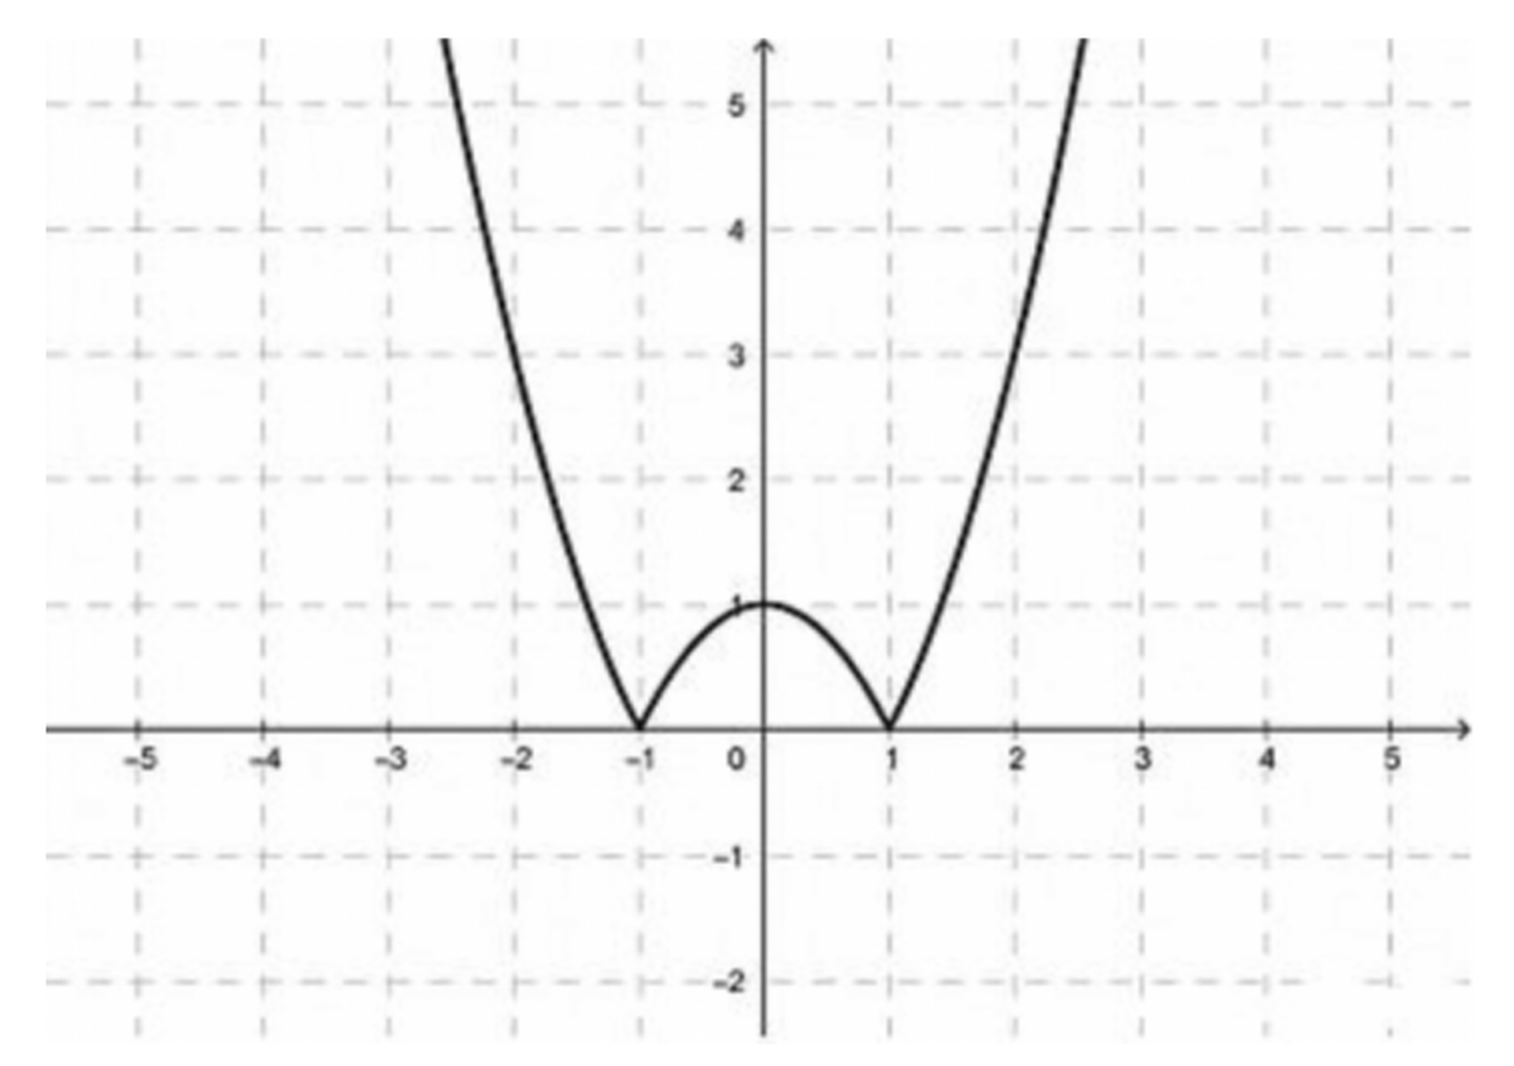
\includegraphics[width=0.55\textwidth]{figures/gao142_q21_para.png}
\end{center}}
\step{(3) 由题意得，$y_1=(2a)^2$，$y_2=(3-a)^2$，}
\step{$y_1<y_2$，即有 $(2a)^2<(3-a)^2$，化简整理得 $(a+3)(a-1)<0$，}
\step{解得实数 $a$ 的取值范围为 $(-3,1)$.}
\solend
\fi

\end{enumerate}

\end{document}
"
% 紧凑版：xelatex "\def\iscompact{1}% 高一142_群峰高级中学_期中.tex
%   —— 高一上数学"2026-2027 年群峰高级中学高一上期中"（试卷版/答案版）
% 试卷版：xelatex 高一142_群峰高级中学_期中.tex
% 答案版：xelatex "\def\isanswer{1}% 高一142_群峰高级中学_期中.tex
%   —— 高一上数学"2026-2027 年群峰高级中学高一上期中"（试卷版/答案版）
% 试卷版：xelatex 高一142_群峰高级中学_期中.tex
% 答案版：xelatex "\def\isanswer{1}\input{高一142_群峰高级中学_期中.tex}"
% 紧凑版：xelatex "\def\iscompact{1}\input{高一142_群峰高级中学_期中.tex}"
%
% ① 原始材料：微信公众号"魔都数学加油站"文章，连载"27学年高一142"，原文标题
% "27学年高一142——2026-2027年上海市群峰高级中学高一上期中"；
% 原文链接：https://mp.weixin.qq.com/s/cc7wnuP4Pk3OjNDV6ihB9A。
% 正文为 9 张 PNG 页（01、02、04、06、07、08、09 为 2560x3620；03、05 为 4762x6735，
% 同一篇各页分辨率不同，逐页按各自分辨率裁图核对），题目下印有【答案】或【解析】，为讲评版。
% 题目、解析均据原图转录；卷面粉红色水印"魔都数学加油站"及公众号页脚未录入。
% 全卷 4 幅插图：第 15 题四幅坐标函数图像选项（04 页，2x2 合并为一张）、
% 第 20 题矩形围栏示意图（07 页）、第 21 题 (2) 空白坐标网格（08 页）、
% 第 21 题抛物线图象（09 页，解析所附图）；均取原卷截图去粉色水印、LANCZOS 放大。
% 题目配图三版都出、解析配图仅答案版出。
%
% 卷首标题：原卷印作"2026-2027 年群峰高级中学高一上期中"（公众号标题中的"上海市"
% 卷面标题行没有，本稿照卷面），年份区间按全稿惯例排 en dash；原卷未印副标题，
% 本卷为期中卷、跨集合与常用逻辑用语／不等式／函数三章，按题目内容补出
% "集合与常用逻辑用语、不等式、函数"（头注说明，与同期中卷口径相同）。
%
% 题号体例：本卷共 19 题——一、填空题 3—12（10 题）、二、选择题 13—16（4 题）、
% 三、解答题 17—21（5 题）。三节分别 \setcounter{enumi}{2}／{12}／{16}。
% 原卷从第 3 题起、无第 1、2 题，本稿保留原题号。
%
% ② 与原卷的排版差异：
%   ① 原文从第 3 题起，本稿保留原题号；原卷未印副标题，本稿按"知识模块"口径补出；
%   ② 逐题答案口径：Q14 原卷把答案 D 印在题干括号内、且题目下无【解析】，本稿括号
%      留空 \mbox{（\quad）}、另提 \ans{D}；Q13／Q15／Q16 答案在【解析】末句"故选 …"
%      （分别为 C／C／A），题干括号留空、不另提 \ans{}；其余各题（Q3—Q12、
%      Q17—Q21）题目下印【解析】、答案融在解析中，不另提 \ans{}；全卷仅 Q14 一处 \ans{}；
%      答案版【答案】/【解析】标记数 = 19（1 个 \ans + 18 个 \solbegin）= 全卷题数；
%   ③ 原卷填空横线按全稿惯例排 \blankline[4.4em]；选择题括号排 \mbox{（\quad）}、
%      每个选项段前按惯例加 \keepwithprev（Q15 四幅图那一枚放在 \begin{center} 之前）；
%      解答题不留作答区、不加 \anspace（原卷为讲评版，与 129／131／132／133／136／140 同）；
%   ④ 原卷数集斜体 $R$（Q5、Q7、Q19、Q21 解析等）按全稿惯例统一改 \R；空集记号
%      \varnothing；绝对值排 \lvert…\rvert，集合描述竖线排 \mid；不等号按全稿惯例
%      排 \leqslant／\geqslant；
%   ⑤ 4 幅插图：Q15 四幅坐标函数图象选项合并裁为一张 \includegraphics（题前
%      \needvspace{9cm}）；Q15 是"二、选择题"节内带大图块的第 3 题（Q13、Q14 在前
%      且无图），另在 \bigsec{二、选择题} 之前加 \needvspace{11cm} 连节标题一起量
%      ——守卫必须放在 \bigsec 之前，放标题之后会让"二、选择题"孤立在页末
%      （B 类，照 高一26／40／59／136／140 成例）；Q20 围栏图与 Q21 网格图置于题干
%      之后（三版都出），Q21 抛物线图置于答案版解析 (2) 与 (3) 之间（仅答案版出）；
%   ⑥ 子题标号按原卷排半角 (1)(2)(3)（与 140／141 同期中卷口径相同）；括注全角／
%      半角逐处照录：Q3"（用含有 m 的代数式表示）"、Q6"（舍）"、Q10"（万元）"、
%      Q18"（请务必书写必要的计算步骤）"、Q20"（墙足够长）"印全角；Q15
%      "$y=a^x(a>0 且 a\neq1)$"、Q10"$y=x^a(a 为常数)$"、Q20"$t=\sqrt{xy}(t>0)$"
%      等数学式内括注印半角；数学式内 CJK 用 \text{…}（否则 FONTCHK 报缺字）；
%   ⑦ 数学式内半角逗号照录（如 Q6"$ax-1=0,a\in\R$"、Q9"$b=2+\sqrt2,a=\sqrt2+1$"、
%      Q16 区间 "$[-1,3]$"、Q21"$y_1<y_2$，即 $(2a)^2<(3-a)^2$" 等）；原卷行末
%      西文句点照录（Q7"(-3,5)."、Q10"125（万元）."、Q19 题干句点、Q20 题干
%      "矩形菜园."与"宽为 y 米."、Q21 题干"对称." 等）；行中全角逗号、分号照录；
%   ⑧ 题干中的中文弯引号：本卷题干与解析通篇未出现中文弯引号，故无此项；
%      圈数字 ①②③ 亦未出现（子题用 (1)(2)(3)）；
%   ⑨ 原卷"图像／图象"两种写法混用，逐处放大核对并照录：Q4 题干与解析作"图象"、
%      Q7 解析作"图象"、Q8 题干作"图像"而解析作"图象"、Q15 题干与解析通篇作
%      "图像"、Q21 题干与解析通篇作"图象"；
%   ⑩ 原卷无红色加粗标签（【解析】均黑色印刷；逐页扫描深红像素为 0），故本卷未用
%      \stepm；黑色常规分步标签（"A 中""C 中""D 中""(1)(2)(3)" 等）按普通 \step
%      行内文字照录；
%   ⑪ 跨页续印按题合并，明细见 ⑥。
%
% ③ 行数复核：一条 \step = 原卷解析的一个印刷行，cases 块作一个印刷行计。逐题数 \step
%   条数，合计 98 条（Q3：1；Q4：2；Q5：3；Q6：4；Q7：5；Q8：2；Q9：4；Q10：3；
%   Q11：4；Q12：3；Q13：5；Q14：0；Q15：10；Q16：4；Q17：10；Q18：3；
%   Q19：10；Q20：13；Q21：12），与原卷印刷行逐题相等。Q14 只把答案印在题干括号、
%   无【解析】，提 \ans{D}、不计入 \step 账；答案版标记数 = 19（1 个 \ans + 18 个
%   \solbegin）= 全卷题数。
%
% ④ 判别式字形：全卷判别式共 3 处——第 7 题【解析】"即判别式△<0"、
%   "即△=(a-1)^2-4×1×4<0" 两处原卷印扁等边三角 $\triangle$，
%   第 11 题【解析】cases 块"△=4a^2-4(a+6)≥0" 一处原卷印等腰偏高的高三角 $\Delta$；
%   逐处放大核对，两形不同、全卷混用，本稿逐处照录不统一（参照 高一141 头注④口径）。
%   子集符号：全卷共 3 处——第 6 题题干"若 B⊆A"、第 6 题【解析】"因为 B⊆A"、
%   第 17 题【解析】(2)"所以 A⊆B"，逐处放大核对，原卷三处均印带下划线的
%   $\subseteq$（不是单线 $\subset$），本稿一律照录 \subseteq；全卷未出现 \subset。
%
% ⑤ 原卷存疑照录（均照录未改，正文对应处另有 % 注）：
%   第 14 题题干括号内原卷印答案 D（非留空），且题目下无【解析】，按"答案印括号且
%      无解析"口径括号留空、另提 \ans{D}；
%   第 15 题【解析】"C 中，由指数函数 … 图像递减得 a>1" 中"递减"与"a>1"
%      自相矛盾（递减应得 0<a<1，疑为"递增"之误），照录；
%   第 16 题选项 B 作 $(-\infty,3]\cup[3,+\infty)$，两端区间并起即全体实数、
%      与正确答案 $[-1,3]$ 不成干扰项（疑为 $(-\infty,-1]\cup[3,+\infty)$ 之误），照录；
%   第 21 题 (2) 空白坐标网格的 x 轴刻度原卷印作"-5 -3 -3 -2 -1 0 1 2 3 4 5"
%      （"-3"重复，疑为"-4"之误），系插图中的印刷内容，取原卷截图照录、不改图。
%
% ⑥ 跨页续印说明：Q7 题干与解析首行在 01 页、解析续至 02 页；Q11 题干与解析
%   4 行在 03 页；Q13 解析前 4 行在 03 页、末句"故选 C."续至 04 页；Q15 题干与
%   四幅图在 04 页、解析前 8 行在 04 页、末 2 行续至 05 页；Q17 解析前 7 行在
%   05 页、后 3 行续至 06 页；Q19 解析前 5 行在 06 页、后 5 行续至 07 页；
%   Q20 解析前 9 行在 07 页、后 4 行续至 08 页；Q21 解析 (1)(2) 9 行在 08 页、
%   抛物线图与 (3) 3 行续至 09 页；本稿按题连排，不丢行。三版切页审计结论见
%   编译自验回报（切页守卫见 ②⑤）。
%
\documentclass[a4paper,11pt]{article}
\usepackage{common}

\begin{document}

\examtitlest[3]{2026--2027 年群峰高级中学高一上期中}{集合与常用逻辑用语、不等式、函数}

\bigsec{一、填空题}

\begin{enumerate}
\setcounter{enumi}{2}

\item 已知 $\log_2 3=m$，则 $\log_3 6=$\blankline[4.4em]（用含有 $m$ 的代数式表示）.

\ifanswer
\solbegin
\step{$\log_3 6=\dfrac{\log_2 6}{\log_2 3}=\dfrac{\log_2 2+\log_2 3}{\log_2 3}=\dfrac{1+m}{m}=\dfrac1m+1$.}
\solend
\fi

\item 若指数函数 $y=a^x$ 的图象经过点 $(3,27)$，则 $a$ 的值为\blankline[4.4em].

\ifanswer
\solbegin
\step{因为指数函数 $y=a^x$ 的图象经过点 $(3,27)$，}
\step{所以 $a^3=27=3^3$，所以 $a=3$.}
\solend
\fi

\item 不等式 $(2x+1)^{\frac13}<(3-x)^{\frac13}$ 的解集为\blankline[4.4em].

\ifanswer
\solbegin
\step{因为幂函数 $f(t)=t^{\frac13}$ 在 $\R$ 上严格增，}
\step{所以原不等式等价于 $2x+1<3-x$，解得 $x<\dfrac23$，}
\step{因此原不等式的解集为 $\left(-\infty,\dfrac23\right)$.}
\solend
\fi

\item 设集合 $A=\{1,-2\}$，$B=\{x\mid ax-1=0,a\in\R\}$，若 $B\subseteq A$，则 $a$ 的值为\blankline[4.4em].% 子集符号原卷印带下划线 $\subseteq$，照录

\ifanswer
\solbegin
\step{因为 $B\subseteq A$，所以 $B=\varnothing$ 或 $\{-2\}$ 或 $\{1\}$ 或 $\{1,-2\}$（舍），}% 子集符号原卷印带下划线 $\subseteq$，照录
\step{若 $B=\varnothing$，则 $a=0$；若 $B=\{1\}$，则 $a=1$；}
\step{若 $B=\{-2\}$，则 $-2a=1$，解得 $a=-\dfrac12$；}
\step{综上，$a=0$ 或 $1$ 或 $-\dfrac12$.}
\solend
\fi

\item 不等式 $x^2+(a-1)x+4>0$ 在 $\R$ 上恒成立，则实数 $a$ 的取值范围是\blankline[4.4em].

\ifanswer
\solbegin
\step{不等式 $x^2+(a-1)x+4>0$，对应的二次函数为 $y=x^2+(a-1)x+4$，}
\step{因此函数图象开口向上，要使不等式对任意实数 $x$ 恒成立，}
\step{需二次函数图象与 $x$ 轴无交点，即判别式 $\triangle<0$，}% 判别式原卷印扁等边三角 $\triangle$，照录
\step{即 $\triangle=(a-1)^2-4\times1\times4<0$，整理得 $a^2-2a-15<0$，}% 判别式原卷印扁等边三角 $\triangle$，照录
\step{解得 $-3<a<5$，故实数 $a$ 的取值范围是 $(-3,5)$.}
\solend
\fi

\item 函数 $f(x)=(5x-3)^a$ 的图像恒过点\blankline[4.4em].% 题干作"图像"、解析作"图象"，原卷混用，逐处照录

\ifanswer
\solbegin
\step{令 $5x-3=1$ 得 $x=\dfrac45$，此时 $f\left(\dfrac45\right)=\left(5\times\dfrac45-3\right)^a=1$，}
\step{所以 $f(x)$ 的图象恒过 $\left(\dfrac45,1\right)$.}
\solend
\fi

\item 若 $a>0$，$b>0$ 且 $\dfrac1a+\dfrac2b=1$，则 $a+b$ 的最小值为\blankline[4.4em].

\ifanswer
\solbegin
\step{因为 $a>0$，$b>0$，$\dfrac1a+\dfrac2b=1$，}
\step{所以 $a+b=(a+b)\left(\dfrac1a+\dfrac2b\right)=1+\dfrac{2a}{b}+\dfrac{b}{a}+2\geqslant3+2\sqrt{\dfrac{2a}{b}\cdot\dfrac{b}{a}}=3+2\sqrt2$，}
\step{当且仅当 $\dfrac{2a}{b}=\dfrac{b}{a}$，即 $b=2+\sqrt2,a=\sqrt2+1$ 时取等号，}
\step{故 $a+b$ 的最小值为 $3+2\sqrt2$.}
\solend
\fi

\item 某药厂研制出一种新型药剂，投放市场后其广告投入 $x$（万元）与药品利润 $y$（万元）存在的关系为 $y=x^a(a\text{ 为常数})$，其中 $x$ 不超过 5 万元. 已知去年投入广告费用为 3 万元时，药品利润为 27 万元，若今年投入广告费用 5 万元，预计今年药品利润为\blankline[4.4em]万元.

\ifanswer
\solbegin
\step{由已知投入广告费用为 3 万元时，药品利润为 27 万元，}
\step{代入 $y=x^a$ 中，即 $3^a=27$，解得 $a=3$，故函数关系式为 $y=x^3$，}
\step{所以当 $x=5$ 时，$y=125$（万元）.}
\solend
\fi

\item 已知方程 $x^2+2ax+a+6=0$ 的两根分别是 $x_1$ 和 $x_2$，且满足 $\dfrac1{x_1}+\dfrac1{x_2}<0$，则实数 $a$ 的取值范围是\blankline[4.4em].

\ifanswer
\solbegin
\step{由于方程 $x^2+2ax+a+6=0$ 的两根分别是 $x_1$ 和 $x_2$，}
\step{则 $\begin{cases}\Delta=4a^2-4(a+6)\geqslant0\\x_1+x_2=-2a\\x_1x_2=a+6\end{cases}$，解得 $a\geqslant3$ 或 $a\leqslant-2$.}% 判别式原卷印等腰偏高的高三角 $\Delta$，照录（与第 7 题扁等边 $\triangle$ 两形混用）
\step{又 $\dfrac1{x_1}+\dfrac1{x_2}<0$，即 $\dfrac{x_1+x_2}{x_1\cdot x_2}<0$，故 $\dfrac{-2a}{a+6}<0$，解得 $a<-6$ 或 $a>0$.}
\step{综上，$a$ 的取值范围是 $(-\infty,-6)\cup[3,+\infty)$.}
\solend
\fi

\item 已知 $b>a>1$，若 $\log_a b-\log_b a=\dfrac32$，$a^b=b^a$，则 $a-b=$\blankline[4.4em].

\ifanswer
\solbegin
\step{因为 $b>a>1$，所以 $\log_a b>1$，}
\step{由 $\log_a b-\log_b a=\log_a b-\dfrac{1}{\log_a b}=\dfrac32$，解得 $\log_a b=2$ 即 $b=a^2$，}
\step{因为 $a^b=b^a=a^{2a}$，所以 $b=2a=a^2$，所以 $a=2$，$b=4$，则 $a-b=-2$.}
\solend
\fi

\end{enumerate}

% 第 15 题四幅图是"二、选择题"节内的大图块；守卫须放在 \bigsec 之前连节标题一起量
\needvspace{11cm}
\bigsec{二、选择题}

\begin{enumerate}
\setcounter{enumi}{12}

\item 若 $a>b$，$c<0$，则下列不等式正确的是\mbox{（\quad）}

\keepwithprev
A. $ab>bc$\qquad B. $a+c<b+c$\qquad C. $ac^2>bc^2$\qquad D. $\dfrac ac>\dfrac bc$

\ifanswer
\solbegin
\step{因为 $a>b$，$c<0$，取 $b=0$，则 $ab=bc=0$，故 $A$ 错误；}
\step{由于 $a>b$，所以 $a+c>b+c$，故 $B$ 错误；}
\step{由 $c<0$ 得 $c^2>0$，所以 $ac^2>bc^2$，故 $C$ 正确；}
\step{由于 $a>b$ 且 $c<0$，所以 $\dfrac ac<\dfrac bc$，故 $D$ 错误.}
\step{故选 $C$.}
\solend
\fi

\item 若 $x>0$，$y>0$，则下列各式中，恒成立的是\mbox{（\quad）}% 原卷题干括号内印答案 D、且题目下无【解析】，本稿括号留空、另提 \ans{D}

\keepwithprev
A. $\lg x+\lg y=\lg(x+y)$\qquad B. $\lg x^2=(\lg x)^2$

C. $\dfrac{\lg x}{\lg y}=\lg(x-y)$\qquad D. $\lg x^{\frac1n}=\dfrac{\lg x}{n}$

\ifanswer
\ans{$D$}
\fi

% 第 15 题四幅坐标函数图象选项是一整块，守卫放在 \item 之前
\needvspace{9cm}
\item 在同一平面直角坐标系中，指数函数 $y=a^x(a>0\text{ 且 }a\neq1)$ 和一次函数 $y=a(x+1)$ 的图像关系可能是\mbox{（\quad）}

\keepwithprev
\begin{center}
% 四幅坐标函数图象选项取原卷 04 页截图去粉色水印、去色，按原卷 2x2 排布合并为一张
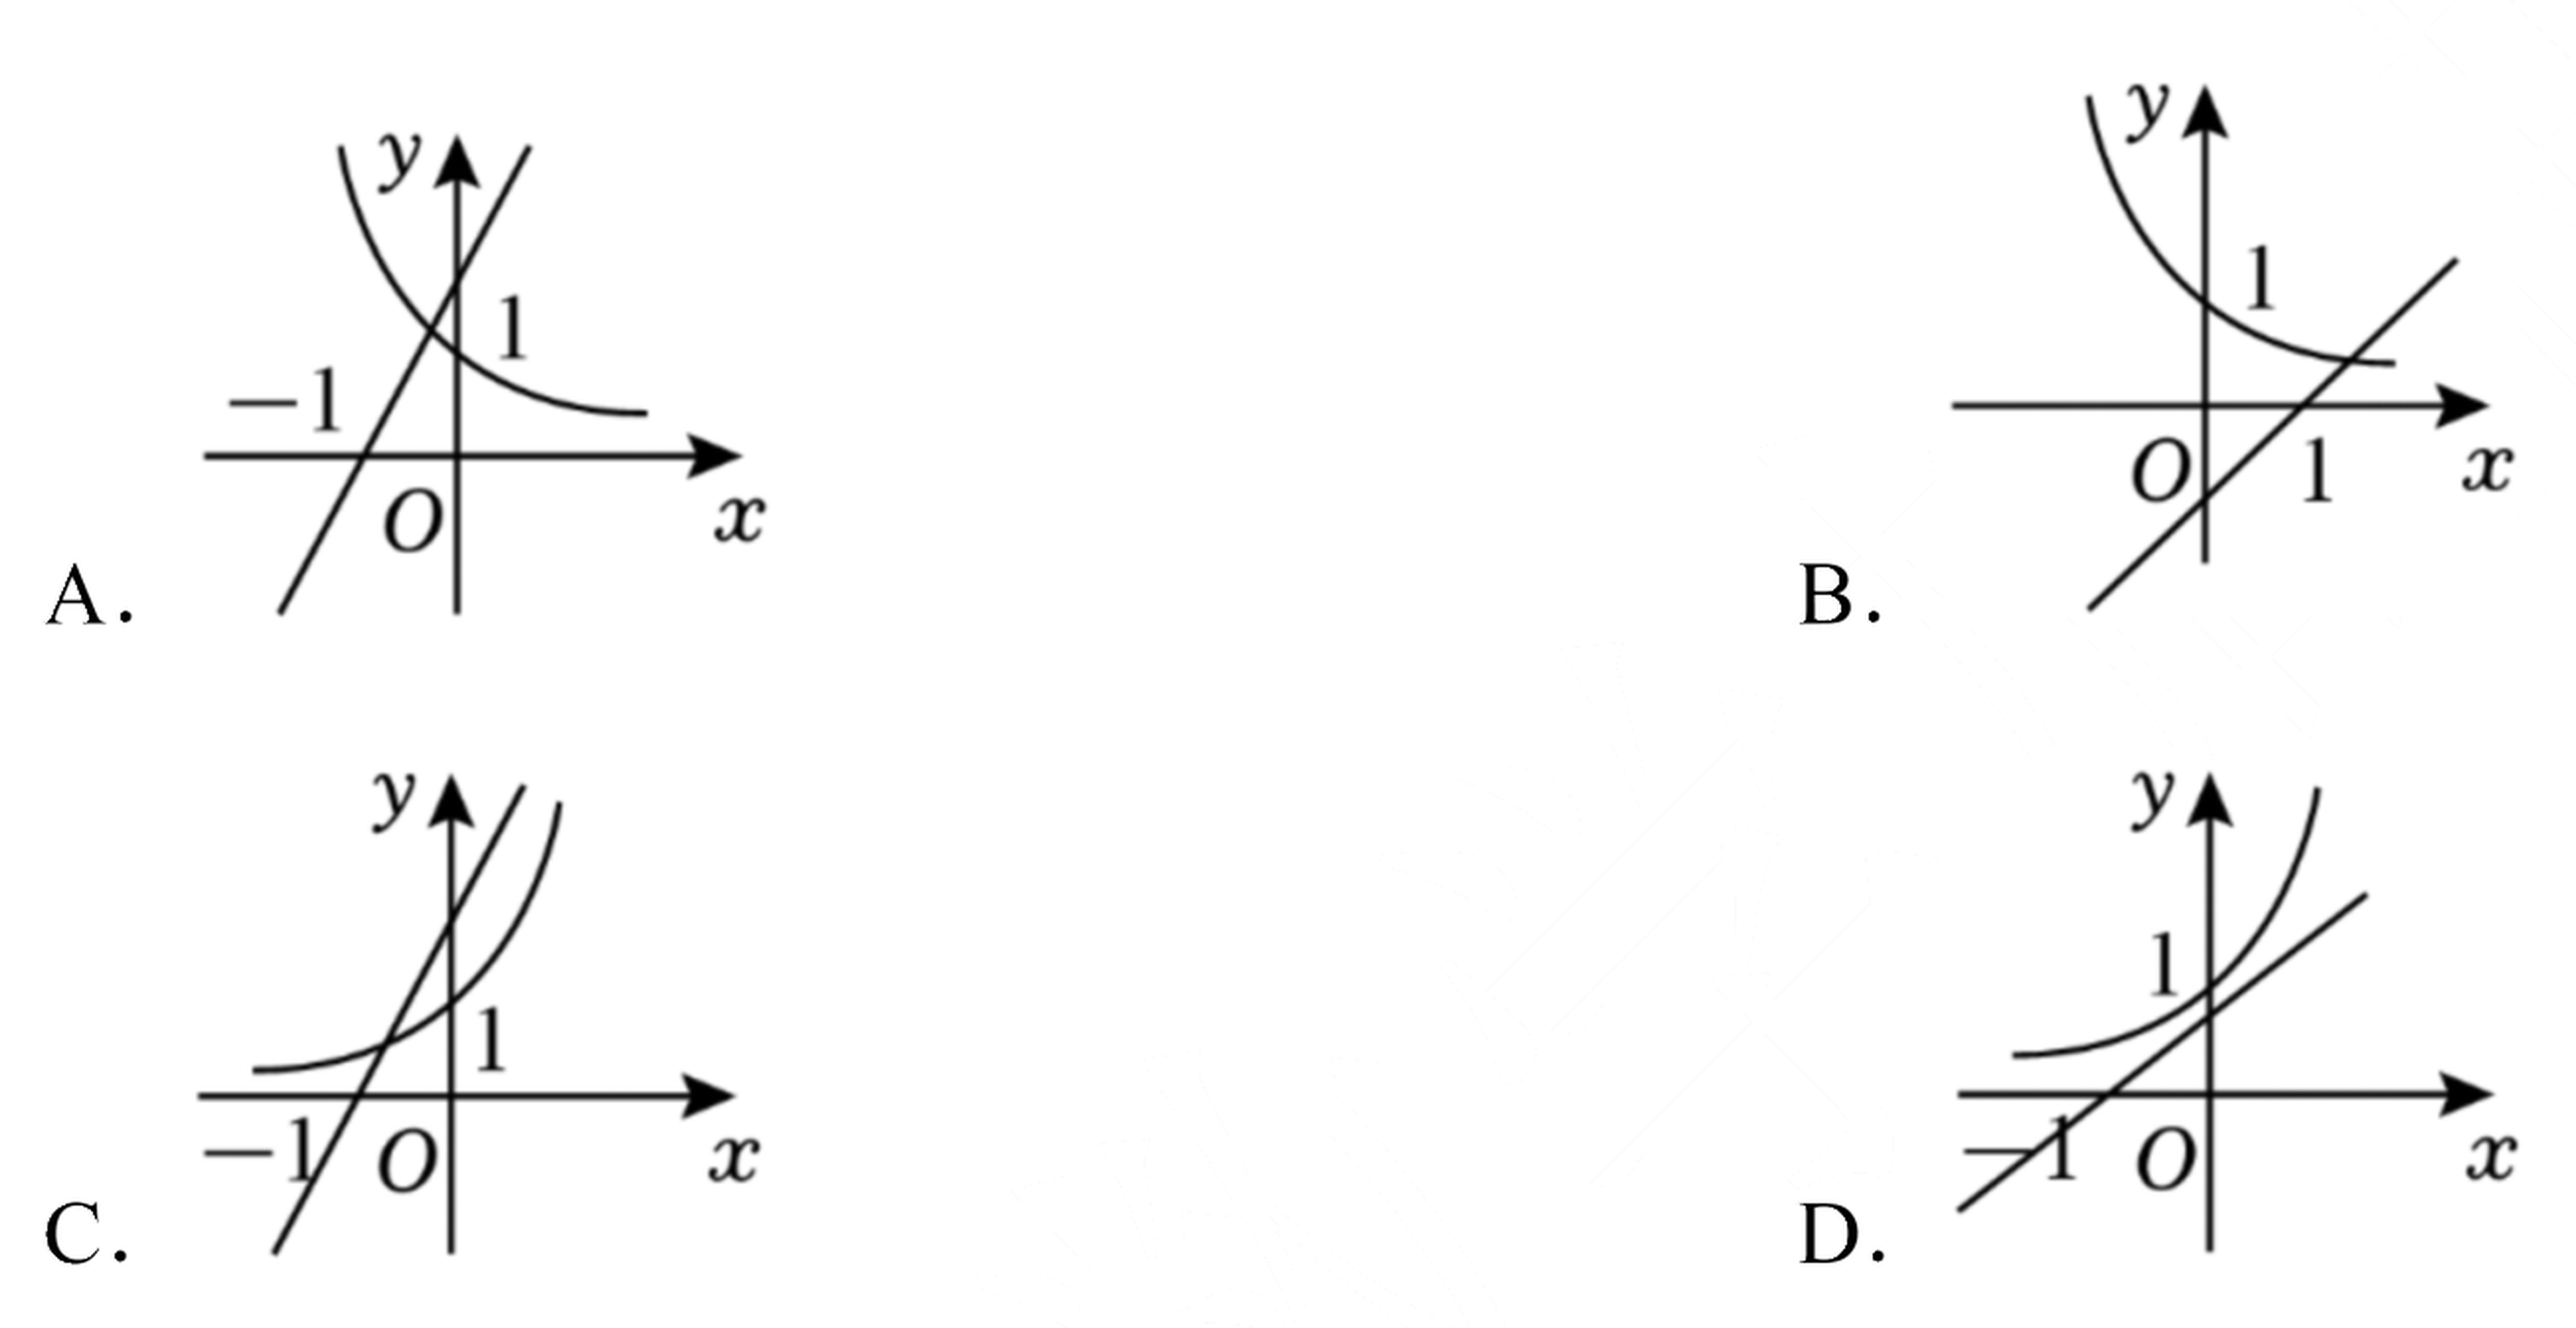
\includegraphics[width=0.80\textwidth]{figures/gao142_q15.png}
\end{center}

\ifanswer
\solbegin
\step{$A$ 中，由指数函数 $y=a^x(a>0\text{ 且 }a\neq1)$ 图像递减得 $0<a<1$，}
\step{而一次函数 $y=a(x+1)$ 的图像与 $y$ 轴交点纵坐标为 $a>1$，二者矛盾，}
\step{所以 $A$ 错；}
\step{由一次函数 $y=a(x+1)$ 的图像与 $x$ 轴交点横坐标为 $-1$，排除 $B$；}
\step{$C$ 中，由指数函数 $y=a^x(a>0\text{ 且 }a\neq1)$ 图像递减得 $a>1$，}% 原卷"递减得 a>1"自相矛盾（递减应得 0<a<1），照录
\step{而一次函数 $y=a(x+1)$ 的图像与 $y$ 轴交点纵坐标为 $a>1$，二者 $a$ 值吻合，}
\step{所以 $C$ 对；}
\step{$D$ 中，由一次函数 $y=a(x+1)$ 的图像得 $a=1$，与 $a>0$ 且 $a\neq1$ 矛盾，}
\step{所以 $D$ 错.}
\step{故选 $C$.}
\solend
\fi

\item 不等式 $\lvert x+1\rvert+\lvert 2-x\rvert\geqslant a^2-2a$ 恒成立，则 $a$ 的取值范围是\mbox{（\quad）}

\keepwithprev
A. $[-1,3]$\qquad B. $(-\infty,3]\cup[3,+\infty)$\qquad C. $(-\infty,3)$\qquad D. $(3,+\infty)$

\ifanswer
\solbegin
\step{因为 $\lvert x+1\rvert+\lvert 2-x\rvert\geqslant\lvert(x+1)+(2-x)\rvert=3$，}
\step{所以 $\lvert x+1\rvert+\lvert 2-x\rvert$ 的最小值为 3，}
\step{因为 $\lvert x+1\rvert+\lvert 2-x\rvert\geqslant a^2-2a$ 恒成立，所以只需 $a^2-2a\leqslant3$，所以 $-1\leqslant a\leqslant3$，}
\step{所以 $a$ 的取值范围为 $[-1,3]$. 故选 $A$.}
\solend
\fi

\end{enumerate}

\bigsec{三、解答题}

\begin{enumerate}
\setcounter{enumi}{16}

\item 已知集合 $A=\left\{x\mid\dfrac{x-3}{x-1}\leqslant0\right\}$，$B=\{x\mid\lvert x-1\rvert<a\}$.

(1) 若 $a=1$，求 $A\cap B$；

(2) 若 $x\in A$ 是 $x\in B$ 的充分条件，求 $a$ 的取值范围.

\ifanswer
\solbegin
\step{(1) 不等式 $\dfrac{x-3}{x-1}\leqslant0$，等价于 $(x-3)(x-1)\leqslant0$ 且 $x-1\neq0$，解得 $1<x\leqslant3$，}
\step{所以 $A=\{x\mid 1<x\leqslant3\}$，}
\step{当 $a=1$ 时，不等式 $\lvert x-1\rvert<a$ 可化为 $\lvert x-1\rvert<1$，所以 $-1<x-1<1$，}
\step{故 $0<x<2$，所以 $B=\{x\mid 0<x<2\}$，}
\step{所以 $A\cap B=\{x\mid 1<x<2\}$；}
\step{(2) 因为 $x\in A$ 是 $x\in B$ 的充分条件，所以 $A\subseteq B$，}% 子集符号原卷印带下划线 $\subseteq$，照录
\step{因为 $A=\{x\mid 1<x\leqslant3\}\neq\varnothing$，所以 $B\neq\varnothing$，故 $a>0$，}
\step{由不等式 $\lvert x-1\rvert<a$，解得 $1-a<x<1+a$，}
\step{所以 $B=\{x\mid 1-a<x<1+a\}$，所以 $\begin{cases}1-a\leqslant1\\1+a>3\end{cases}$，解得 $a>2$，}
\step{所以 $a$ 的取值范围为 $(2,+\infty)$.}
\solend
\fi

\item 计算下列式子的值（请务必书写必要的计算步骤）

(1) $27^{\frac13}+\left(\dfrac76\right)^0+\sqrt{(3-\pi)^2}$；

(2) $\lg25+\lg4+7^{\log_7 2}-\log_2 3\times\log_3 4+\log_3 9$.

\ifanswer
\solbegin
\step{(1) $27^{\frac13}+\left(\dfrac76\right)^0+\sqrt{(3-\pi)^2}=3^{3\times\frac13}+1+\lvert 3-\pi\rvert=3+1+\pi-3=\pi+1$；}
\step{(2) 原式 $=\lg(25\times4)+2-\dfrac{\lg3}{\lg2}\times\dfrac{\lg4}{\lg3}+2=\lg100+2-\dfrac{2\lg2}{\lg2}+2$}
\step{$=2+2-2+2=4$.}
\solend
\fi

\item 已知关于 $x$ 的不等式 $mx^2-(3m^2-m+2)x+6m-2\geqslant0$.

(1) 当 $m=2$ 时，求关于 $x$ 的不等式的解集；

(2) 当 $m>0$ 时，求关于 $x$ 的不等式的解集.

\ifanswer
\solbegin
\step{(1) $m=2$ 时，不等式为 $x^2-6x+5\geqslant0$，即 $(x-1)(x-5)\geqslant0$，}
\step{解得 $x\leqslant1$ 或 $x\geqslant5$，所以不等式的解集是 $\{x\mid x\leqslant1$ 或 $x\geqslant5\}$.}
\step{(2) $m>0$ 时，不等式可化为 $(mx-2)[x-(3m-1)]\geqslant0$，}
\step{即 $\left(x-\dfrac2m\right)[x-(3m-1)]\geqslant0$，}
\step{若 $m=1$，则不等式为 $(x-2)^2\geqslant0$，解得 $x\in\R$；}
\step{若 $0<m<1$，则 $\dfrac2m>3m-1$，解不等式得 $x\geqslant\dfrac2m$ 或 $x\leqslant3m-1$；}
\step{若 $m>1$，则 $\dfrac2m<3m-1$，解不等式得 $x\geqslant3m-1$ 或 $x\leqslant\dfrac2m$；}
\step{综上，$0<m<1$ 时，不等式的解集是 $\{x\mid x\leqslant3m-1$ 或 $x\geqslant\dfrac2m\}$；}
\step{$m=1$ 时，不等式的解集为 $\R$；}
\step{$m>1$ 时，不等式的解集是 $\{x\mid x\leqslant\dfrac2m$ 或 $x\geqslant3m-1\}$.}
\solend
\fi

\item 如图，某人计划用篱笆围成一个一边靠墙（墙足够长）的矩形菜园. 设菜园的长为 $x$ 米，宽为 $y$ 米.

\begin{center}
% 矩形围栏示意图取原卷 07 页截图去粉色水印、去色、LANCZOS 放大；题目配图，三版都出
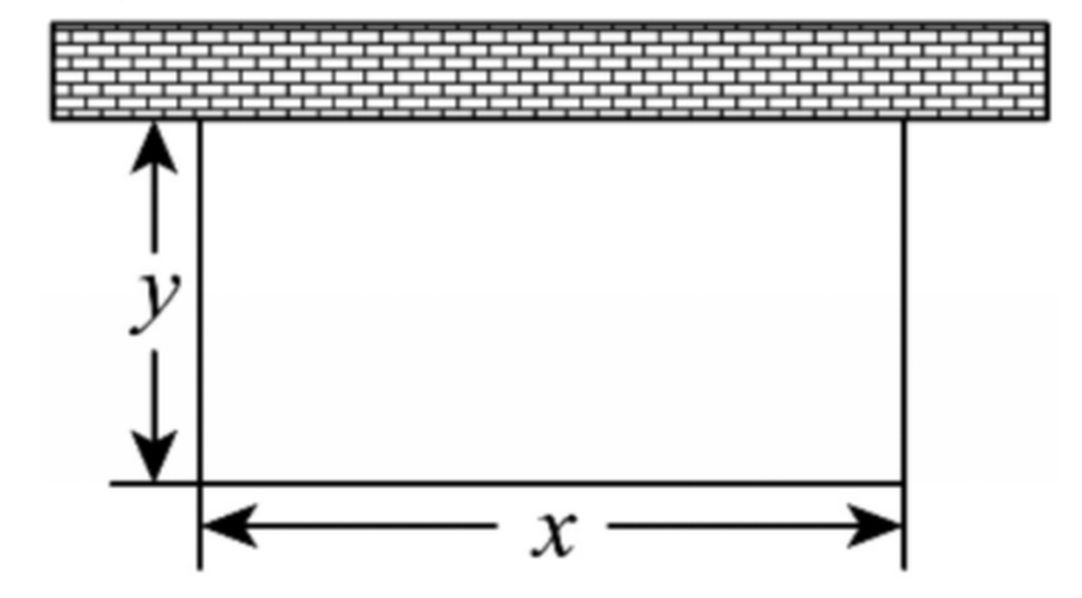
\includegraphics[width=0.42\textwidth]{figures/gao142_q20.png}
\end{center}

(1) 若菜园面积为 72 平方米，则 $x$、$y$ 为何值时，所用篱笆总长最小？

(2) 若 $x$、$y$ 满足 $x+y-xy+63=0$，则菜园面积最小为多少平方米？

\ifanswer
\solbegin
\step{(1) 由题意得，菜园的面积 $S=xy=72$，且 $x>0$，$y>0$，}
\step{所用篱笆总长 $L=x+2y$，}
\step{由基本不等式得 $x+2y\geqslant2\sqrt{x\cdot2y}=2\sqrt{2xy}=2\sqrt{2\times72}=24$，}
\step{当且仅当 $x=2y$ 时取等号，}
\step{联立 $\begin{cases}xy=72\\x=2y\end{cases}$，解得 $\begin{cases}x=12\\y=6\end{cases}$，}
\step{所以当 $x=12$，$y=6$ 时，所用篱笆总长最小；}
\step{(2) 由题意得 $x>0$，$y>0$，且满足 $x+y-xy+63=0$，即 $x+y=xy-63$，}
\step{由基本不等式得 $x+y\geqslant2\sqrt{xy}$，当且仅当 $x=y$ 时取等号，}
\step{所以 $xy-63\geqslant2\sqrt{xy}$. 令 $t=\sqrt{xy}(t>0)$，则 $xy=t^2$，}
\step{上述不等式可化为 $t^2-2t-63\geqslant0$，即 $(t-9)(t+7)\geqslant0$，}
\step{因为 $t>0$，所以 $t+7>0$，故 $t-9\geqslant0$，解得 $t\geqslant9$，所以 $\sqrt{xy}\geqslant9$，}
\step{即 $xy\geqslant81$，当且仅当 $x=y=9$ 时取等号，此时满足 $9+9-81+63=0$，}
\step{所以菜园面积最小为 81 平方米.}
\solend
\fi

\item 已知幂函数 $f(x)=(m^2-3m+3)x^m$ 的图象关于 $y$ 轴对称.

(1) 求实数 $m$ 的值；

(2) 在平面直角坐标系中作出函数 $y=\lvert f(x)-1\rvert$ 的图象；

(3) 已知点 $A(2a,y_1)$ 与点 $B(3-a,y_2)$ 都在幂函数 $y=x^2$ 的图象上. 若 $y_1<y_2$，求实数 $a$ 的取值范围.

\begin{center}
% 空白坐标网格取原卷 08 页截图去粉色水印、去色、LANCZOS 放大；题目配图，三版都出
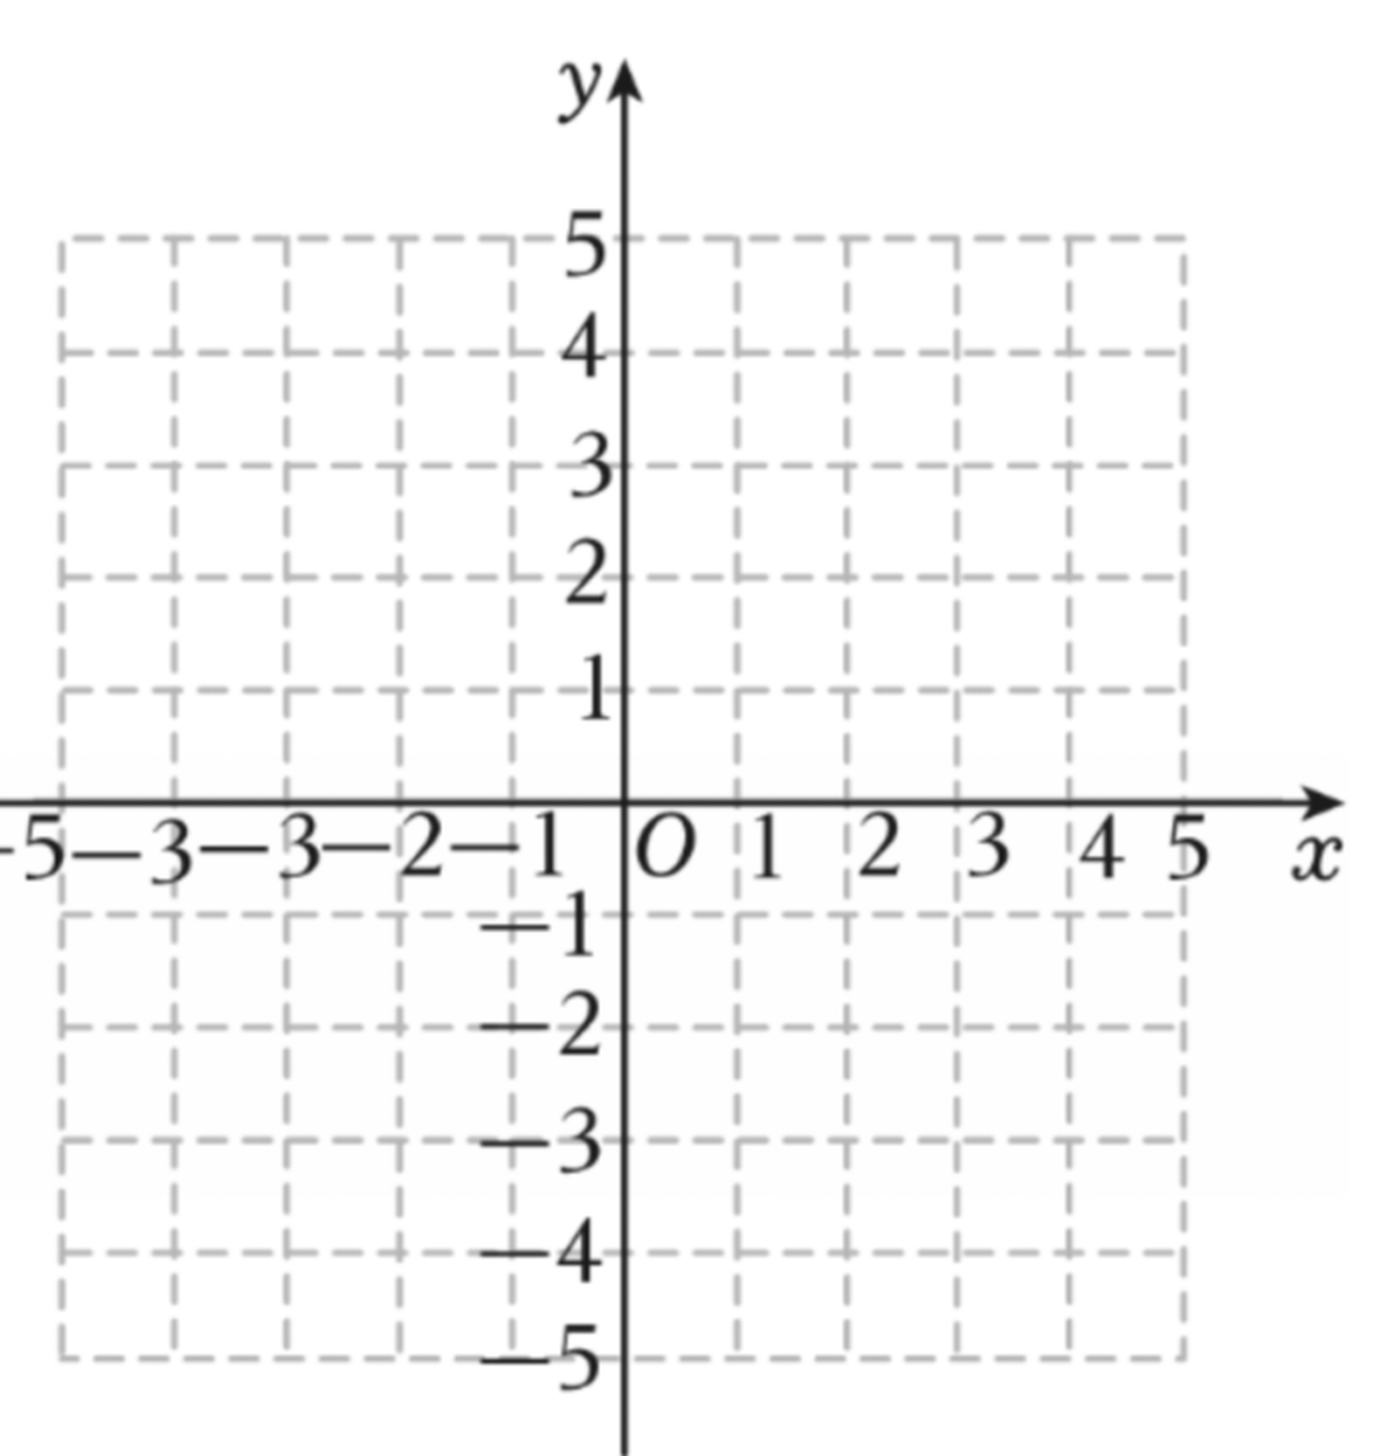
\includegraphics[width=0.52\textwidth]{figures/gao142_q21_grid.png}
\end{center}

\ifanswer
\solbegin
\step{(1) 由题意幂函数 $f(x)=(m^2-3m+3)x^m$，}
\step{故 $m^2-3m+3=1$，解得 $m=1$ 或 $m=2$，}
\step{又 $f(x)$ 图象关于 $y$ 轴对称，即 $f(x)$ 是偶函数，}
\step{当 $m=1$ 时，$f(x)=x$ 是奇函数，不满足条件，舍去；}
\step{当 $m=2$ 时，$f(x)=x^2$ 是偶函数，满足条件，故 $m=2$；}
\step{(2) 由 (1) 得，$\lvert f(x)-1\rvert=\lvert x^2-1\rvert$，}
\step{先画 $y=x^2-1$，开口向上的抛物线，顶点 $(0,-1)$，零点 $x=\pm1$，}
\step{再将 $x$ 轴下方的部分沿 $x$ 轴翻折到上方即为 $y=\lvert x^2-1\rvert$ 的图象，}
\step{图象如图所示.}
\par{\leftskip=0pt
\begin{center}
% 抛物线图象取原卷 09 页截图去粉色水印、去色、LANCZOS 放大；解析所附配图，仅答案版出
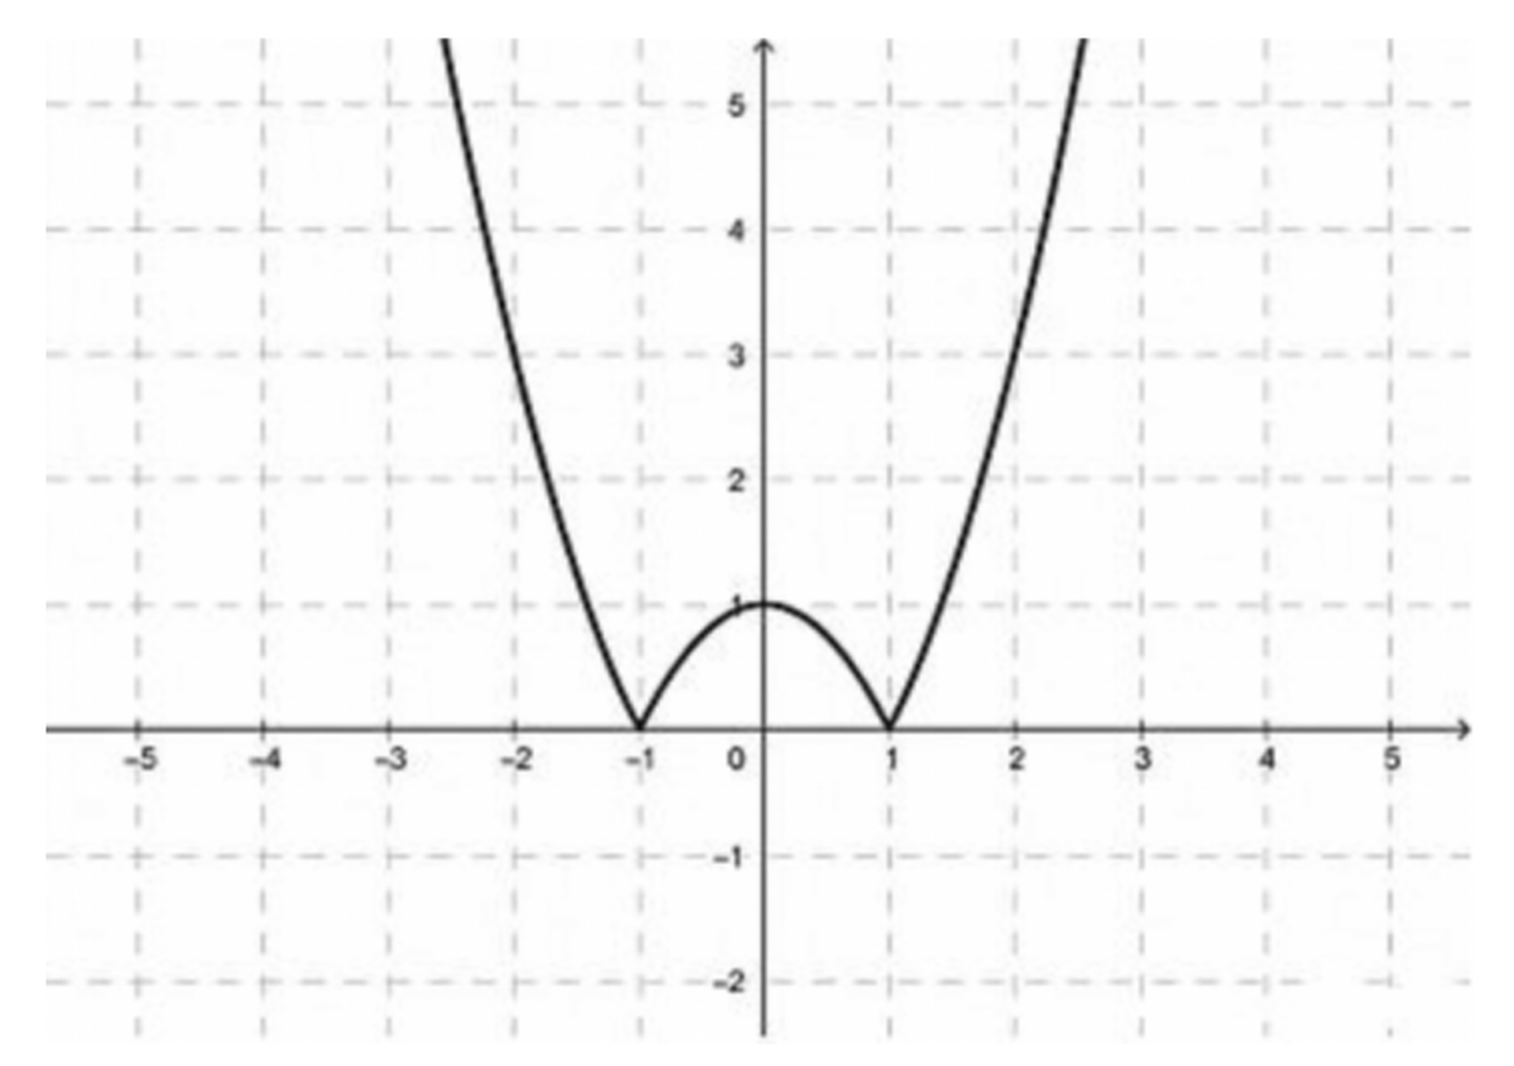
\includegraphics[width=0.55\textwidth]{figures/gao142_q21_para.png}
\end{center}}
\step{(3) 由题意得，$y_1=(2a)^2$，$y_2=(3-a)^2$，}
\step{$y_1<y_2$，即有 $(2a)^2<(3-a)^2$，化简整理得 $(a+3)(a-1)<0$，}
\step{解得实数 $a$ 的取值范围为 $(-3,1)$.}
\solend
\fi

\end{enumerate}

\end{document}
"
% 紧凑版：xelatex "\def\iscompact{1}% 高一142_群峰高级中学_期中.tex
%   —— 高一上数学"2026-2027 年群峰高级中学高一上期中"（试卷版/答案版）
% 试卷版：xelatex 高一142_群峰高级中学_期中.tex
% 答案版：xelatex "\def\isanswer{1}\input{高一142_群峰高级中学_期中.tex}"
% 紧凑版：xelatex "\def\iscompact{1}\input{高一142_群峰高级中学_期中.tex}"
%
% ① 原始材料：微信公众号"魔都数学加油站"文章，连载"27学年高一142"，原文标题
% "27学年高一142——2026-2027年上海市群峰高级中学高一上期中"；
% 原文链接：https://mp.weixin.qq.com/s/cc7wnuP4Pk3OjNDV6ihB9A。
% 正文为 9 张 PNG 页（01、02、04、06、07、08、09 为 2560x3620；03、05 为 4762x6735，
% 同一篇各页分辨率不同，逐页按各自分辨率裁图核对），题目下印有【答案】或【解析】，为讲评版。
% 题目、解析均据原图转录；卷面粉红色水印"魔都数学加油站"及公众号页脚未录入。
% 全卷 4 幅插图：第 15 题四幅坐标函数图像选项（04 页，2x2 合并为一张）、
% 第 20 题矩形围栏示意图（07 页）、第 21 题 (2) 空白坐标网格（08 页）、
% 第 21 题抛物线图象（09 页，解析所附图）；均取原卷截图去粉色水印、LANCZOS 放大。
% 题目配图三版都出、解析配图仅答案版出。
%
% 卷首标题：原卷印作"2026-2027 年群峰高级中学高一上期中"（公众号标题中的"上海市"
% 卷面标题行没有，本稿照卷面），年份区间按全稿惯例排 en dash；原卷未印副标题，
% 本卷为期中卷、跨集合与常用逻辑用语／不等式／函数三章，按题目内容补出
% "集合与常用逻辑用语、不等式、函数"（头注说明，与同期中卷口径相同）。
%
% 题号体例：本卷共 19 题——一、填空题 3—12（10 题）、二、选择题 13—16（4 题）、
% 三、解答题 17—21（5 题）。三节分别 \setcounter{enumi}{2}／{12}／{16}。
% 原卷从第 3 题起、无第 1、2 题，本稿保留原题号。
%
% ② 与原卷的排版差异：
%   ① 原文从第 3 题起，本稿保留原题号；原卷未印副标题，本稿按"知识模块"口径补出；
%   ② 逐题答案口径：Q14 原卷把答案 D 印在题干括号内、且题目下无【解析】，本稿括号
%      留空 \mbox{（\quad）}、另提 \ans{D}；Q13／Q15／Q16 答案在【解析】末句"故选 …"
%      （分别为 C／C／A），题干括号留空、不另提 \ans{}；其余各题（Q3—Q12、
%      Q17—Q21）题目下印【解析】、答案融在解析中，不另提 \ans{}；全卷仅 Q14 一处 \ans{}；
%      答案版【答案】/【解析】标记数 = 19（1 个 \ans + 18 个 \solbegin）= 全卷题数；
%   ③ 原卷填空横线按全稿惯例排 \blankline[4.4em]；选择题括号排 \mbox{（\quad）}、
%      每个选项段前按惯例加 \keepwithprev（Q15 四幅图那一枚放在 \begin{center} 之前）；
%      解答题不留作答区、不加 \anspace（原卷为讲评版，与 129／131／132／133／136／140 同）；
%   ④ 原卷数集斜体 $R$（Q5、Q7、Q19、Q21 解析等）按全稿惯例统一改 \R；空集记号
%      \varnothing；绝对值排 \lvert…\rvert，集合描述竖线排 \mid；不等号按全稿惯例
%      排 \leqslant／\geqslant；
%   ⑤ 4 幅插图：Q15 四幅坐标函数图象选项合并裁为一张 \includegraphics（题前
%      \needvspace{9cm}）；Q15 是"二、选择题"节内带大图块的第 3 题（Q13、Q14 在前
%      且无图），另在 \bigsec{二、选择题} 之前加 \needvspace{11cm} 连节标题一起量
%      ——守卫必须放在 \bigsec 之前，放标题之后会让"二、选择题"孤立在页末
%      （B 类，照 高一26／40／59／136／140 成例）；Q20 围栏图与 Q21 网格图置于题干
%      之后（三版都出），Q21 抛物线图置于答案版解析 (2) 与 (3) 之间（仅答案版出）；
%   ⑥ 子题标号按原卷排半角 (1)(2)(3)（与 140／141 同期中卷口径相同）；括注全角／
%      半角逐处照录：Q3"（用含有 m 的代数式表示）"、Q6"（舍）"、Q10"（万元）"、
%      Q18"（请务必书写必要的计算步骤）"、Q20"（墙足够长）"印全角；Q15
%      "$y=a^x(a>0 且 a\neq1)$"、Q10"$y=x^a(a 为常数)$"、Q20"$t=\sqrt{xy}(t>0)$"
%      等数学式内括注印半角；数学式内 CJK 用 \text{…}（否则 FONTCHK 报缺字）；
%   ⑦ 数学式内半角逗号照录（如 Q6"$ax-1=0,a\in\R$"、Q9"$b=2+\sqrt2,a=\sqrt2+1$"、
%      Q16 区间 "$[-1,3]$"、Q21"$y_1<y_2$，即 $(2a)^2<(3-a)^2$" 等）；原卷行末
%      西文句点照录（Q7"(-3,5)."、Q10"125（万元）."、Q19 题干句点、Q20 题干
%      "矩形菜园."与"宽为 y 米."、Q21 题干"对称." 等）；行中全角逗号、分号照录；
%   ⑧ 题干中的中文弯引号：本卷题干与解析通篇未出现中文弯引号，故无此项；
%      圈数字 ①②③ 亦未出现（子题用 (1)(2)(3)）；
%   ⑨ 原卷"图像／图象"两种写法混用，逐处放大核对并照录：Q4 题干与解析作"图象"、
%      Q7 解析作"图象"、Q8 题干作"图像"而解析作"图象"、Q15 题干与解析通篇作
%      "图像"、Q21 题干与解析通篇作"图象"；
%   ⑩ 原卷无红色加粗标签（【解析】均黑色印刷；逐页扫描深红像素为 0），故本卷未用
%      \stepm；黑色常规分步标签（"A 中""C 中""D 中""(1)(2)(3)" 等）按普通 \step
%      行内文字照录；
%   ⑪ 跨页续印按题合并，明细见 ⑥。
%
% ③ 行数复核：一条 \step = 原卷解析的一个印刷行，cases 块作一个印刷行计。逐题数 \step
%   条数，合计 98 条（Q3：1；Q4：2；Q5：3；Q6：4；Q7：5；Q8：2；Q9：4；Q10：3；
%   Q11：4；Q12：3；Q13：5；Q14：0；Q15：10；Q16：4；Q17：10；Q18：3；
%   Q19：10；Q20：13；Q21：12），与原卷印刷行逐题相等。Q14 只把答案印在题干括号、
%   无【解析】，提 \ans{D}、不计入 \step 账；答案版标记数 = 19（1 个 \ans + 18 个
%   \solbegin）= 全卷题数。
%
% ④ 判别式字形：全卷判别式共 3 处——第 7 题【解析】"即判别式△<0"、
%   "即△=(a-1)^2-4×1×4<0" 两处原卷印扁等边三角 $\triangle$，
%   第 11 题【解析】cases 块"△=4a^2-4(a+6)≥0" 一处原卷印等腰偏高的高三角 $\Delta$；
%   逐处放大核对，两形不同、全卷混用，本稿逐处照录不统一（参照 高一141 头注④口径）。
%   子集符号：全卷共 3 处——第 6 题题干"若 B⊆A"、第 6 题【解析】"因为 B⊆A"、
%   第 17 题【解析】(2)"所以 A⊆B"，逐处放大核对，原卷三处均印带下划线的
%   $\subseteq$（不是单线 $\subset$），本稿一律照录 \subseteq；全卷未出现 \subset。
%
% ⑤ 原卷存疑照录（均照录未改，正文对应处另有 % 注）：
%   第 14 题题干括号内原卷印答案 D（非留空），且题目下无【解析】，按"答案印括号且
%      无解析"口径括号留空、另提 \ans{D}；
%   第 15 题【解析】"C 中，由指数函数 … 图像递减得 a>1" 中"递减"与"a>1"
%      自相矛盾（递减应得 0<a<1，疑为"递增"之误），照录；
%   第 16 题选项 B 作 $(-\infty,3]\cup[3,+\infty)$，两端区间并起即全体实数、
%      与正确答案 $[-1,3]$ 不成干扰项（疑为 $(-\infty,-1]\cup[3,+\infty)$ 之误），照录；
%   第 21 题 (2) 空白坐标网格的 x 轴刻度原卷印作"-5 -3 -3 -2 -1 0 1 2 3 4 5"
%      （"-3"重复，疑为"-4"之误），系插图中的印刷内容，取原卷截图照录、不改图。
%
% ⑥ 跨页续印说明：Q7 题干与解析首行在 01 页、解析续至 02 页；Q11 题干与解析
%   4 行在 03 页；Q13 解析前 4 行在 03 页、末句"故选 C."续至 04 页；Q15 题干与
%   四幅图在 04 页、解析前 8 行在 04 页、末 2 行续至 05 页；Q17 解析前 7 行在
%   05 页、后 3 行续至 06 页；Q19 解析前 5 行在 06 页、后 5 行续至 07 页；
%   Q20 解析前 9 行在 07 页、后 4 行续至 08 页；Q21 解析 (1)(2) 9 行在 08 页、
%   抛物线图与 (3) 3 行续至 09 页；本稿按题连排，不丢行。三版切页审计结论见
%   编译自验回报（切页守卫见 ②⑤）。
%
\documentclass[a4paper,11pt]{article}
\usepackage{common}

\begin{document}

\examtitlest[3]{2026--2027 年群峰高级中学高一上期中}{集合与常用逻辑用语、不等式、函数}

\bigsec{一、填空题}

\begin{enumerate}
\setcounter{enumi}{2}

\item 已知 $\log_2 3=m$，则 $\log_3 6=$\blankline[4.4em]（用含有 $m$ 的代数式表示）.

\ifanswer
\solbegin
\step{$\log_3 6=\dfrac{\log_2 6}{\log_2 3}=\dfrac{\log_2 2+\log_2 3}{\log_2 3}=\dfrac{1+m}{m}=\dfrac1m+1$.}
\solend
\fi

\item 若指数函数 $y=a^x$ 的图象经过点 $(3,27)$，则 $a$ 的值为\blankline[4.4em].

\ifanswer
\solbegin
\step{因为指数函数 $y=a^x$ 的图象经过点 $(3,27)$，}
\step{所以 $a^3=27=3^3$，所以 $a=3$.}
\solend
\fi

\item 不等式 $(2x+1)^{\frac13}<(3-x)^{\frac13}$ 的解集为\blankline[4.4em].

\ifanswer
\solbegin
\step{因为幂函数 $f(t)=t^{\frac13}$ 在 $\R$ 上严格增，}
\step{所以原不等式等价于 $2x+1<3-x$，解得 $x<\dfrac23$，}
\step{因此原不等式的解集为 $\left(-\infty,\dfrac23\right)$.}
\solend
\fi

\item 设集合 $A=\{1,-2\}$，$B=\{x\mid ax-1=0,a\in\R\}$，若 $B\subseteq A$，则 $a$ 的值为\blankline[4.4em].% 子集符号原卷印带下划线 $\subseteq$，照录

\ifanswer
\solbegin
\step{因为 $B\subseteq A$，所以 $B=\varnothing$ 或 $\{-2\}$ 或 $\{1\}$ 或 $\{1,-2\}$（舍），}% 子集符号原卷印带下划线 $\subseteq$，照录
\step{若 $B=\varnothing$，则 $a=0$；若 $B=\{1\}$，则 $a=1$；}
\step{若 $B=\{-2\}$，则 $-2a=1$，解得 $a=-\dfrac12$；}
\step{综上，$a=0$ 或 $1$ 或 $-\dfrac12$.}
\solend
\fi

\item 不等式 $x^2+(a-1)x+4>0$ 在 $\R$ 上恒成立，则实数 $a$ 的取值范围是\blankline[4.4em].

\ifanswer
\solbegin
\step{不等式 $x^2+(a-1)x+4>0$，对应的二次函数为 $y=x^2+(a-1)x+4$，}
\step{因此函数图象开口向上，要使不等式对任意实数 $x$ 恒成立，}
\step{需二次函数图象与 $x$ 轴无交点，即判别式 $\triangle<0$，}% 判别式原卷印扁等边三角 $\triangle$，照录
\step{即 $\triangle=(a-1)^2-4\times1\times4<0$，整理得 $a^2-2a-15<0$，}% 判别式原卷印扁等边三角 $\triangle$，照录
\step{解得 $-3<a<5$，故实数 $a$ 的取值范围是 $(-3,5)$.}
\solend
\fi

\item 函数 $f(x)=(5x-3)^a$ 的图像恒过点\blankline[4.4em].% 题干作"图像"、解析作"图象"，原卷混用，逐处照录

\ifanswer
\solbegin
\step{令 $5x-3=1$ 得 $x=\dfrac45$，此时 $f\left(\dfrac45\right)=\left(5\times\dfrac45-3\right)^a=1$，}
\step{所以 $f(x)$ 的图象恒过 $\left(\dfrac45,1\right)$.}
\solend
\fi

\item 若 $a>0$，$b>0$ 且 $\dfrac1a+\dfrac2b=1$，则 $a+b$ 的最小值为\blankline[4.4em].

\ifanswer
\solbegin
\step{因为 $a>0$，$b>0$，$\dfrac1a+\dfrac2b=1$，}
\step{所以 $a+b=(a+b)\left(\dfrac1a+\dfrac2b\right)=1+\dfrac{2a}{b}+\dfrac{b}{a}+2\geqslant3+2\sqrt{\dfrac{2a}{b}\cdot\dfrac{b}{a}}=3+2\sqrt2$，}
\step{当且仅当 $\dfrac{2a}{b}=\dfrac{b}{a}$，即 $b=2+\sqrt2,a=\sqrt2+1$ 时取等号，}
\step{故 $a+b$ 的最小值为 $3+2\sqrt2$.}
\solend
\fi

\item 某药厂研制出一种新型药剂，投放市场后其广告投入 $x$（万元）与药品利润 $y$（万元）存在的关系为 $y=x^a(a\text{ 为常数})$，其中 $x$ 不超过 5 万元. 已知去年投入广告费用为 3 万元时，药品利润为 27 万元，若今年投入广告费用 5 万元，预计今年药品利润为\blankline[4.4em]万元.

\ifanswer
\solbegin
\step{由已知投入广告费用为 3 万元时，药品利润为 27 万元，}
\step{代入 $y=x^a$ 中，即 $3^a=27$，解得 $a=3$，故函数关系式为 $y=x^3$，}
\step{所以当 $x=5$ 时，$y=125$（万元）.}
\solend
\fi

\item 已知方程 $x^2+2ax+a+6=0$ 的两根分别是 $x_1$ 和 $x_2$，且满足 $\dfrac1{x_1}+\dfrac1{x_2}<0$，则实数 $a$ 的取值范围是\blankline[4.4em].

\ifanswer
\solbegin
\step{由于方程 $x^2+2ax+a+6=0$ 的两根分别是 $x_1$ 和 $x_2$，}
\step{则 $\begin{cases}\Delta=4a^2-4(a+6)\geqslant0\\x_1+x_2=-2a\\x_1x_2=a+6\end{cases}$，解得 $a\geqslant3$ 或 $a\leqslant-2$.}% 判别式原卷印等腰偏高的高三角 $\Delta$，照录（与第 7 题扁等边 $\triangle$ 两形混用）
\step{又 $\dfrac1{x_1}+\dfrac1{x_2}<0$，即 $\dfrac{x_1+x_2}{x_1\cdot x_2}<0$，故 $\dfrac{-2a}{a+6}<0$，解得 $a<-6$ 或 $a>0$.}
\step{综上，$a$ 的取值范围是 $(-\infty,-6)\cup[3,+\infty)$.}
\solend
\fi

\item 已知 $b>a>1$，若 $\log_a b-\log_b a=\dfrac32$，$a^b=b^a$，则 $a-b=$\blankline[4.4em].

\ifanswer
\solbegin
\step{因为 $b>a>1$，所以 $\log_a b>1$，}
\step{由 $\log_a b-\log_b a=\log_a b-\dfrac{1}{\log_a b}=\dfrac32$，解得 $\log_a b=2$ 即 $b=a^2$，}
\step{因为 $a^b=b^a=a^{2a}$，所以 $b=2a=a^2$，所以 $a=2$，$b=4$，则 $a-b=-2$.}
\solend
\fi

\end{enumerate}

% 第 15 题四幅图是"二、选择题"节内的大图块；守卫须放在 \bigsec 之前连节标题一起量
\needvspace{11cm}
\bigsec{二、选择题}

\begin{enumerate}
\setcounter{enumi}{12}

\item 若 $a>b$，$c<0$，则下列不等式正确的是\mbox{（\quad）}

\keepwithprev
A. $ab>bc$\qquad B. $a+c<b+c$\qquad C. $ac^2>bc^2$\qquad D. $\dfrac ac>\dfrac bc$

\ifanswer
\solbegin
\step{因为 $a>b$，$c<0$，取 $b=0$，则 $ab=bc=0$，故 $A$ 错误；}
\step{由于 $a>b$，所以 $a+c>b+c$，故 $B$ 错误；}
\step{由 $c<0$ 得 $c^2>0$，所以 $ac^2>bc^2$，故 $C$ 正确；}
\step{由于 $a>b$ 且 $c<0$，所以 $\dfrac ac<\dfrac bc$，故 $D$ 错误.}
\step{故选 $C$.}
\solend
\fi

\item 若 $x>0$，$y>0$，则下列各式中，恒成立的是\mbox{（\quad）}% 原卷题干括号内印答案 D、且题目下无【解析】，本稿括号留空、另提 \ans{D}

\keepwithprev
A. $\lg x+\lg y=\lg(x+y)$\qquad B. $\lg x^2=(\lg x)^2$

C. $\dfrac{\lg x}{\lg y}=\lg(x-y)$\qquad D. $\lg x^{\frac1n}=\dfrac{\lg x}{n}$

\ifanswer
\ans{$D$}
\fi

% 第 15 题四幅坐标函数图象选项是一整块，守卫放在 \item 之前
\needvspace{9cm}
\item 在同一平面直角坐标系中，指数函数 $y=a^x(a>0\text{ 且 }a\neq1)$ 和一次函数 $y=a(x+1)$ 的图像关系可能是\mbox{（\quad）}

\keepwithprev
\begin{center}
% 四幅坐标函数图象选项取原卷 04 页截图去粉色水印、去色，按原卷 2x2 排布合并为一张
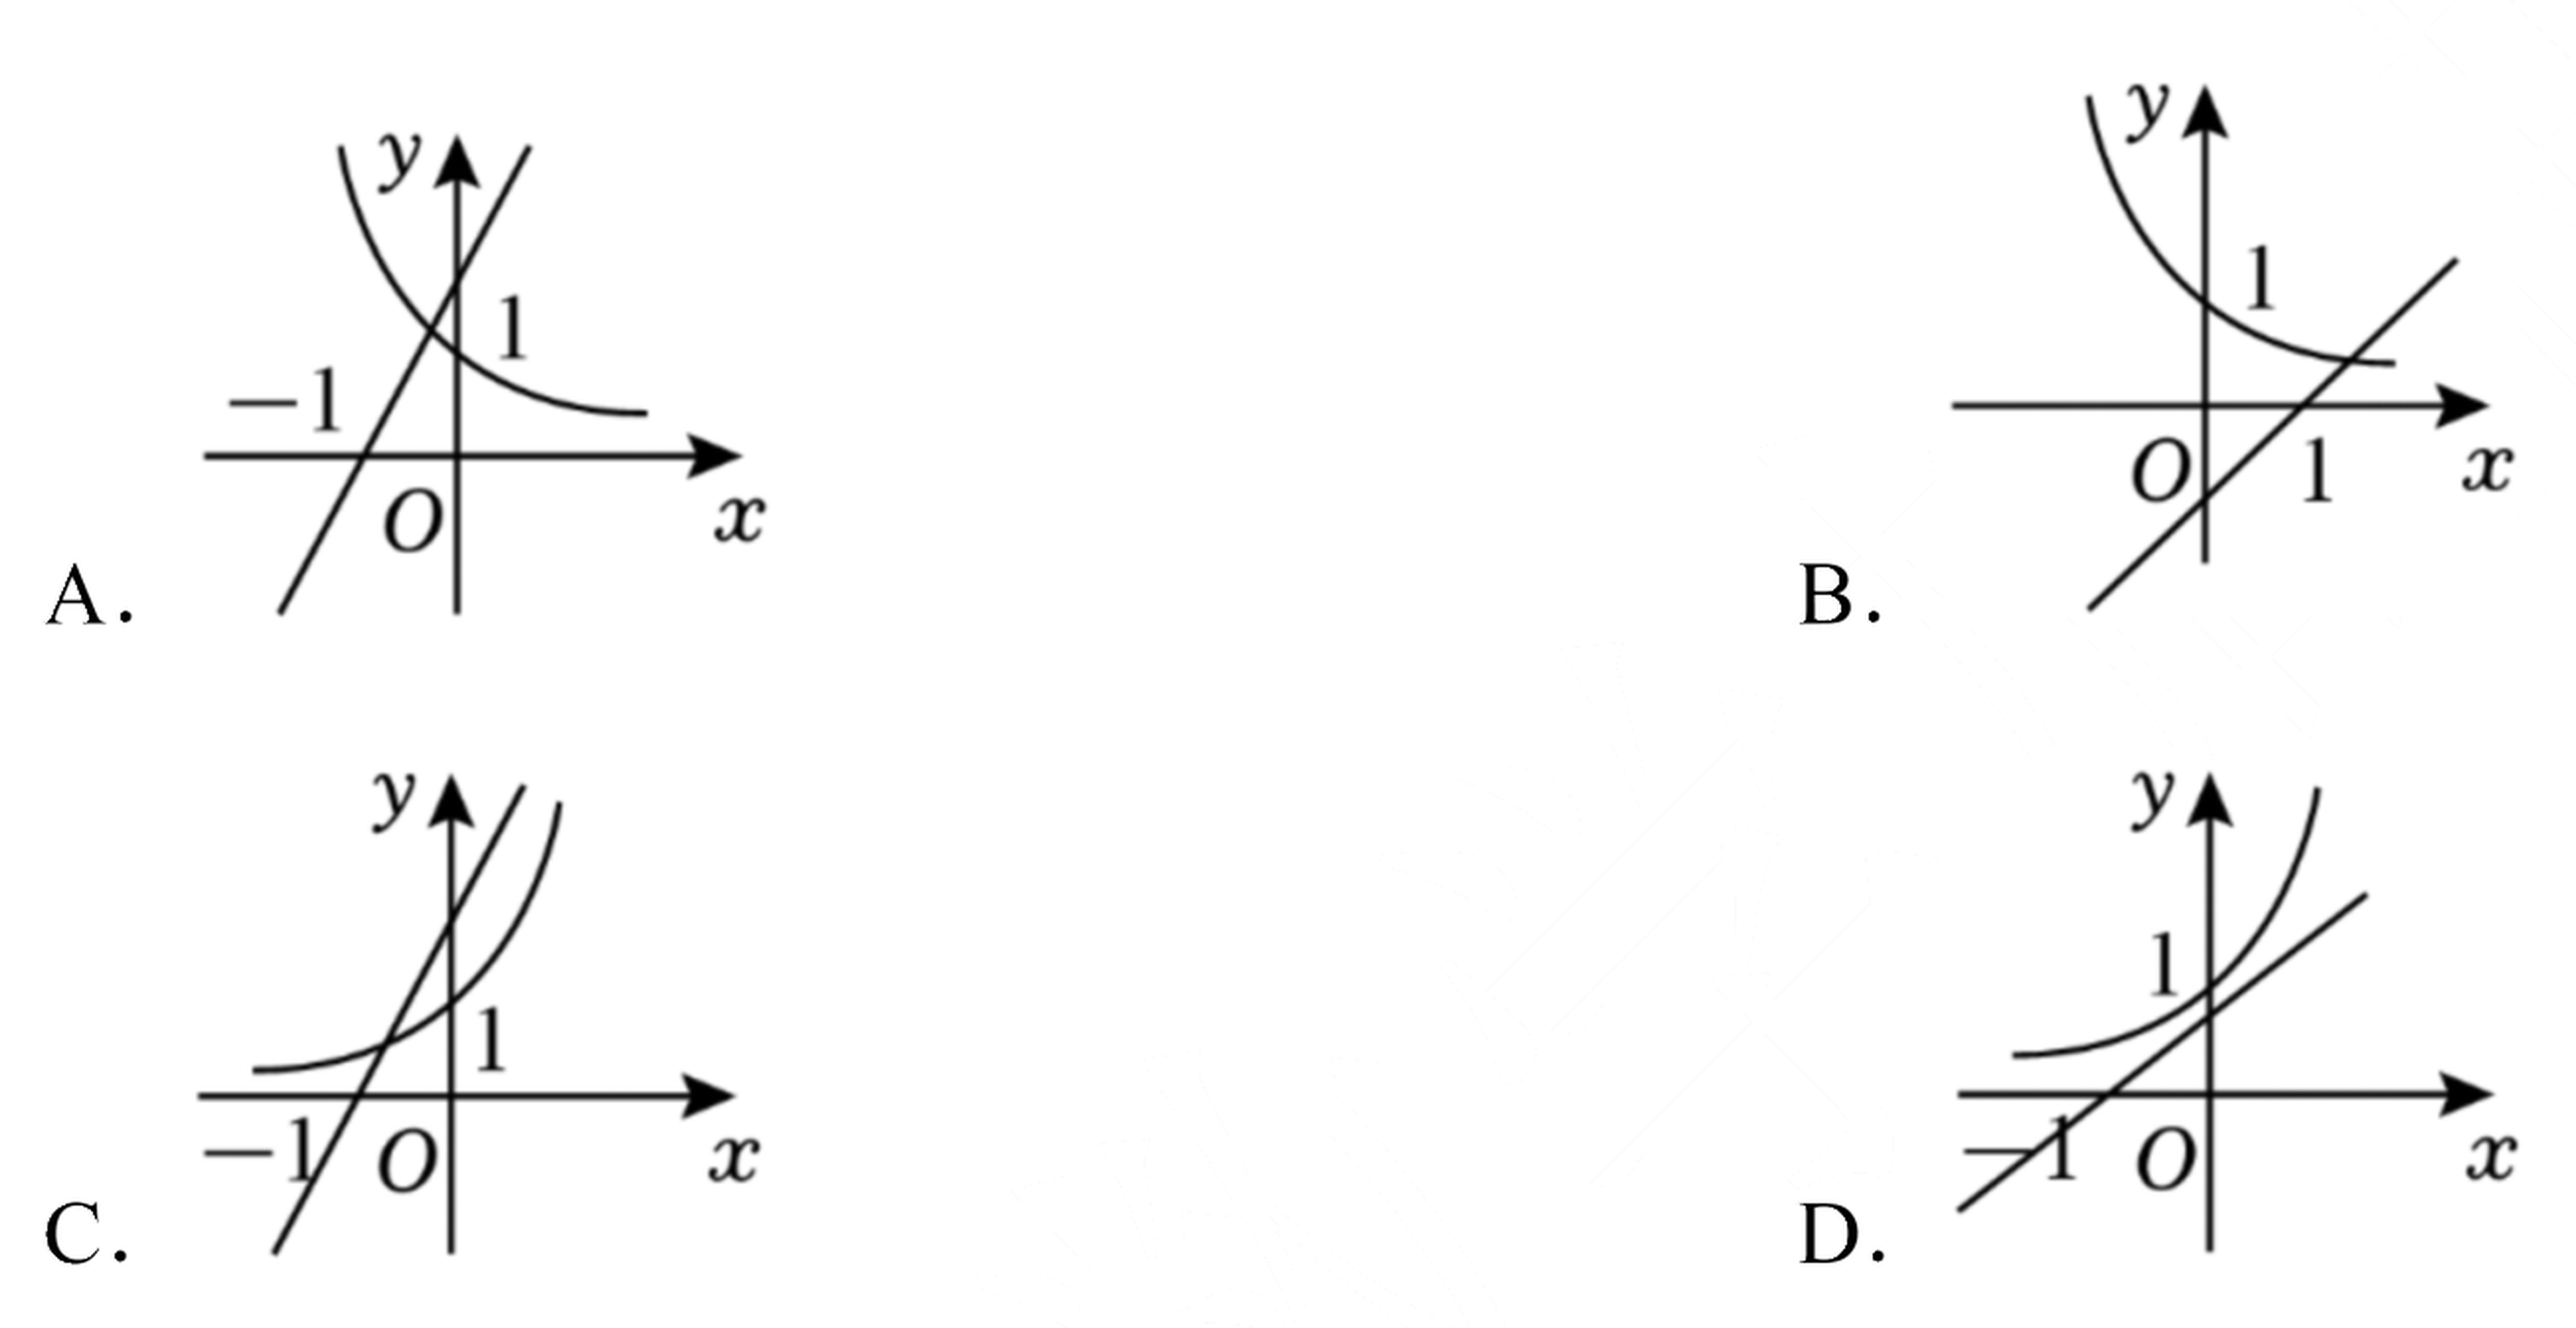
\includegraphics[width=0.80\textwidth]{figures/gao142_q15.png}
\end{center}

\ifanswer
\solbegin
\step{$A$ 中，由指数函数 $y=a^x(a>0\text{ 且 }a\neq1)$ 图像递减得 $0<a<1$，}
\step{而一次函数 $y=a(x+1)$ 的图像与 $y$ 轴交点纵坐标为 $a>1$，二者矛盾，}
\step{所以 $A$ 错；}
\step{由一次函数 $y=a(x+1)$ 的图像与 $x$ 轴交点横坐标为 $-1$，排除 $B$；}
\step{$C$ 中，由指数函数 $y=a^x(a>0\text{ 且 }a\neq1)$ 图像递减得 $a>1$，}% 原卷"递减得 a>1"自相矛盾（递减应得 0<a<1），照录
\step{而一次函数 $y=a(x+1)$ 的图像与 $y$ 轴交点纵坐标为 $a>1$，二者 $a$ 值吻合，}
\step{所以 $C$ 对；}
\step{$D$ 中，由一次函数 $y=a(x+1)$ 的图像得 $a=1$，与 $a>0$ 且 $a\neq1$ 矛盾，}
\step{所以 $D$ 错.}
\step{故选 $C$.}
\solend
\fi

\item 不等式 $\lvert x+1\rvert+\lvert 2-x\rvert\geqslant a^2-2a$ 恒成立，则 $a$ 的取值范围是\mbox{（\quad）}

\keepwithprev
A. $[-1,3]$\qquad B. $(-\infty,3]\cup[3,+\infty)$\qquad C. $(-\infty,3)$\qquad D. $(3,+\infty)$

\ifanswer
\solbegin
\step{因为 $\lvert x+1\rvert+\lvert 2-x\rvert\geqslant\lvert(x+1)+(2-x)\rvert=3$，}
\step{所以 $\lvert x+1\rvert+\lvert 2-x\rvert$ 的最小值为 3，}
\step{因为 $\lvert x+1\rvert+\lvert 2-x\rvert\geqslant a^2-2a$ 恒成立，所以只需 $a^2-2a\leqslant3$，所以 $-1\leqslant a\leqslant3$，}
\step{所以 $a$ 的取值范围为 $[-1,3]$. 故选 $A$.}
\solend
\fi

\end{enumerate}

\bigsec{三、解答题}

\begin{enumerate}
\setcounter{enumi}{16}

\item 已知集合 $A=\left\{x\mid\dfrac{x-3}{x-1}\leqslant0\right\}$，$B=\{x\mid\lvert x-1\rvert<a\}$.

(1) 若 $a=1$，求 $A\cap B$；

(2) 若 $x\in A$ 是 $x\in B$ 的充分条件，求 $a$ 的取值范围.

\ifanswer
\solbegin
\step{(1) 不等式 $\dfrac{x-3}{x-1}\leqslant0$，等价于 $(x-3)(x-1)\leqslant0$ 且 $x-1\neq0$，解得 $1<x\leqslant3$，}
\step{所以 $A=\{x\mid 1<x\leqslant3\}$，}
\step{当 $a=1$ 时，不等式 $\lvert x-1\rvert<a$ 可化为 $\lvert x-1\rvert<1$，所以 $-1<x-1<1$，}
\step{故 $0<x<2$，所以 $B=\{x\mid 0<x<2\}$，}
\step{所以 $A\cap B=\{x\mid 1<x<2\}$；}
\step{(2) 因为 $x\in A$ 是 $x\in B$ 的充分条件，所以 $A\subseteq B$，}% 子集符号原卷印带下划线 $\subseteq$，照录
\step{因为 $A=\{x\mid 1<x\leqslant3\}\neq\varnothing$，所以 $B\neq\varnothing$，故 $a>0$，}
\step{由不等式 $\lvert x-1\rvert<a$，解得 $1-a<x<1+a$，}
\step{所以 $B=\{x\mid 1-a<x<1+a\}$，所以 $\begin{cases}1-a\leqslant1\\1+a>3\end{cases}$，解得 $a>2$，}
\step{所以 $a$ 的取值范围为 $(2,+\infty)$.}
\solend
\fi

\item 计算下列式子的值（请务必书写必要的计算步骤）

(1) $27^{\frac13}+\left(\dfrac76\right)^0+\sqrt{(3-\pi)^2}$；

(2) $\lg25+\lg4+7^{\log_7 2}-\log_2 3\times\log_3 4+\log_3 9$.

\ifanswer
\solbegin
\step{(1) $27^{\frac13}+\left(\dfrac76\right)^0+\sqrt{(3-\pi)^2}=3^{3\times\frac13}+1+\lvert 3-\pi\rvert=3+1+\pi-3=\pi+1$；}
\step{(2) 原式 $=\lg(25\times4)+2-\dfrac{\lg3}{\lg2}\times\dfrac{\lg4}{\lg3}+2=\lg100+2-\dfrac{2\lg2}{\lg2}+2$}
\step{$=2+2-2+2=4$.}
\solend
\fi

\item 已知关于 $x$ 的不等式 $mx^2-(3m^2-m+2)x+6m-2\geqslant0$.

(1) 当 $m=2$ 时，求关于 $x$ 的不等式的解集；

(2) 当 $m>0$ 时，求关于 $x$ 的不等式的解集.

\ifanswer
\solbegin
\step{(1) $m=2$ 时，不等式为 $x^2-6x+5\geqslant0$，即 $(x-1)(x-5)\geqslant0$，}
\step{解得 $x\leqslant1$ 或 $x\geqslant5$，所以不等式的解集是 $\{x\mid x\leqslant1$ 或 $x\geqslant5\}$.}
\step{(2) $m>0$ 时，不等式可化为 $(mx-2)[x-(3m-1)]\geqslant0$，}
\step{即 $\left(x-\dfrac2m\right)[x-(3m-1)]\geqslant0$，}
\step{若 $m=1$，则不等式为 $(x-2)^2\geqslant0$，解得 $x\in\R$；}
\step{若 $0<m<1$，则 $\dfrac2m>3m-1$，解不等式得 $x\geqslant\dfrac2m$ 或 $x\leqslant3m-1$；}
\step{若 $m>1$，则 $\dfrac2m<3m-1$，解不等式得 $x\geqslant3m-1$ 或 $x\leqslant\dfrac2m$；}
\step{综上，$0<m<1$ 时，不等式的解集是 $\{x\mid x\leqslant3m-1$ 或 $x\geqslant\dfrac2m\}$；}
\step{$m=1$ 时，不等式的解集为 $\R$；}
\step{$m>1$ 时，不等式的解集是 $\{x\mid x\leqslant\dfrac2m$ 或 $x\geqslant3m-1\}$.}
\solend
\fi

\item 如图，某人计划用篱笆围成一个一边靠墙（墙足够长）的矩形菜园. 设菜园的长为 $x$ 米，宽为 $y$ 米.

\begin{center}
% 矩形围栏示意图取原卷 07 页截图去粉色水印、去色、LANCZOS 放大；题目配图，三版都出
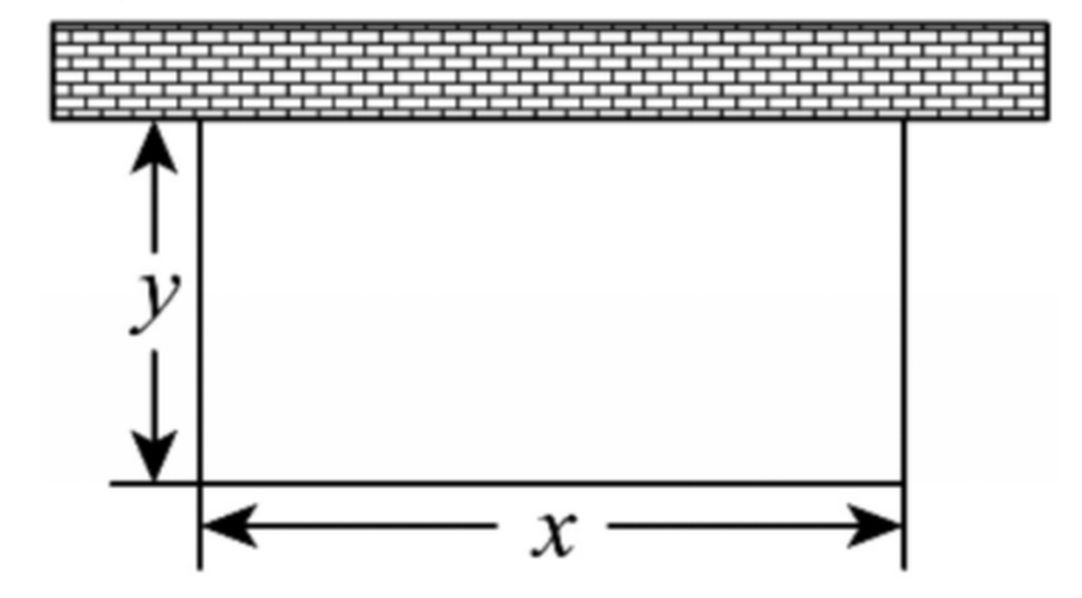
\includegraphics[width=0.42\textwidth]{figures/gao142_q20.png}
\end{center}

(1) 若菜园面积为 72 平方米，则 $x$、$y$ 为何值时，所用篱笆总长最小？

(2) 若 $x$、$y$ 满足 $x+y-xy+63=0$，则菜园面积最小为多少平方米？

\ifanswer
\solbegin
\step{(1) 由题意得，菜园的面积 $S=xy=72$，且 $x>0$，$y>0$，}
\step{所用篱笆总长 $L=x+2y$，}
\step{由基本不等式得 $x+2y\geqslant2\sqrt{x\cdot2y}=2\sqrt{2xy}=2\sqrt{2\times72}=24$，}
\step{当且仅当 $x=2y$ 时取等号，}
\step{联立 $\begin{cases}xy=72\\x=2y\end{cases}$，解得 $\begin{cases}x=12\\y=6\end{cases}$，}
\step{所以当 $x=12$，$y=6$ 时，所用篱笆总长最小；}
\step{(2) 由题意得 $x>0$，$y>0$，且满足 $x+y-xy+63=0$，即 $x+y=xy-63$，}
\step{由基本不等式得 $x+y\geqslant2\sqrt{xy}$，当且仅当 $x=y$ 时取等号，}
\step{所以 $xy-63\geqslant2\sqrt{xy}$. 令 $t=\sqrt{xy}(t>0)$，则 $xy=t^2$，}
\step{上述不等式可化为 $t^2-2t-63\geqslant0$，即 $(t-9)(t+7)\geqslant0$，}
\step{因为 $t>0$，所以 $t+7>0$，故 $t-9\geqslant0$，解得 $t\geqslant9$，所以 $\sqrt{xy}\geqslant9$，}
\step{即 $xy\geqslant81$，当且仅当 $x=y=9$ 时取等号，此时满足 $9+9-81+63=0$，}
\step{所以菜园面积最小为 81 平方米.}
\solend
\fi

\item 已知幂函数 $f(x)=(m^2-3m+3)x^m$ 的图象关于 $y$ 轴对称.

(1) 求实数 $m$ 的值；

(2) 在平面直角坐标系中作出函数 $y=\lvert f(x)-1\rvert$ 的图象；

(3) 已知点 $A(2a,y_1)$ 与点 $B(3-a,y_2)$ 都在幂函数 $y=x^2$ 的图象上. 若 $y_1<y_2$，求实数 $a$ 的取值范围.

\begin{center}
% 空白坐标网格取原卷 08 页截图去粉色水印、去色、LANCZOS 放大；题目配图，三版都出
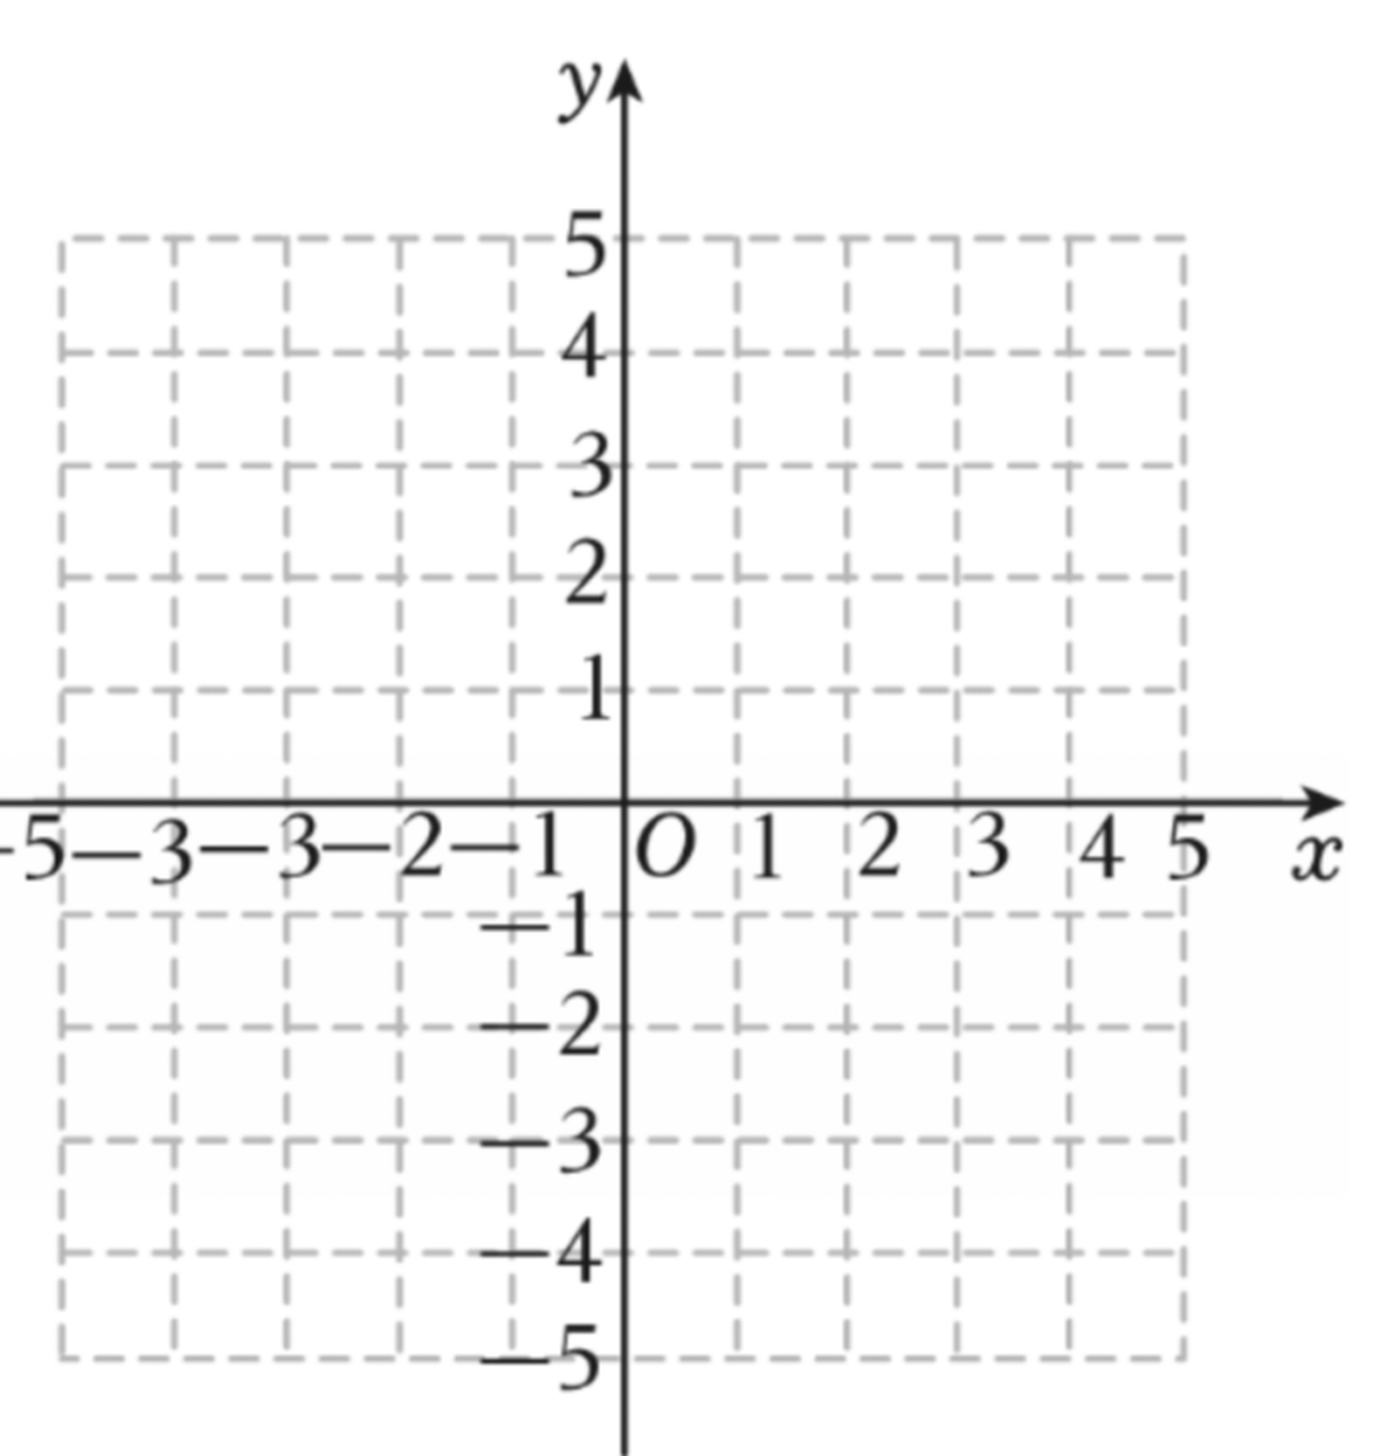
\includegraphics[width=0.52\textwidth]{figures/gao142_q21_grid.png}
\end{center}

\ifanswer
\solbegin
\step{(1) 由题意幂函数 $f(x)=(m^2-3m+3)x^m$，}
\step{故 $m^2-3m+3=1$，解得 $m=1$ 或 $m=2$，}
\step{又 $f(x)$ 图象关于 $y$ 轴对称，即 $f(x)$ 是偶函数，}
\step{当 $m=1$ 时，$f(x)=x$ 是奇函数，不满足条件，舍去；}
\step{当 $m=2$ 时，$f(x)=x^2$ 是偶函数，满足条件，故 $m=2$；}
\step{(2) 由 (1) 得，$\lvert f(x)-1\rvert=\lvert x^2-1\rvert$，}
\step{先画 $y=x^2-1$，开口向上的抛物线，顶点 $(0,-1)$，零点 $x=\pm1$，}
\step{再将 $x$ 轴下方的部分沿 $x$ 轴翻折到上方即为 $y=\lvert x^2-1\rvert$ 的图象，}
\step{图象如图所示.}
\par{\leftskip=0pt
\begin{center}
% 抛物线图象取原卷 09 页截图去粉色水印、去色、LANCZOS 放大；解析所附配图，仅答案版出
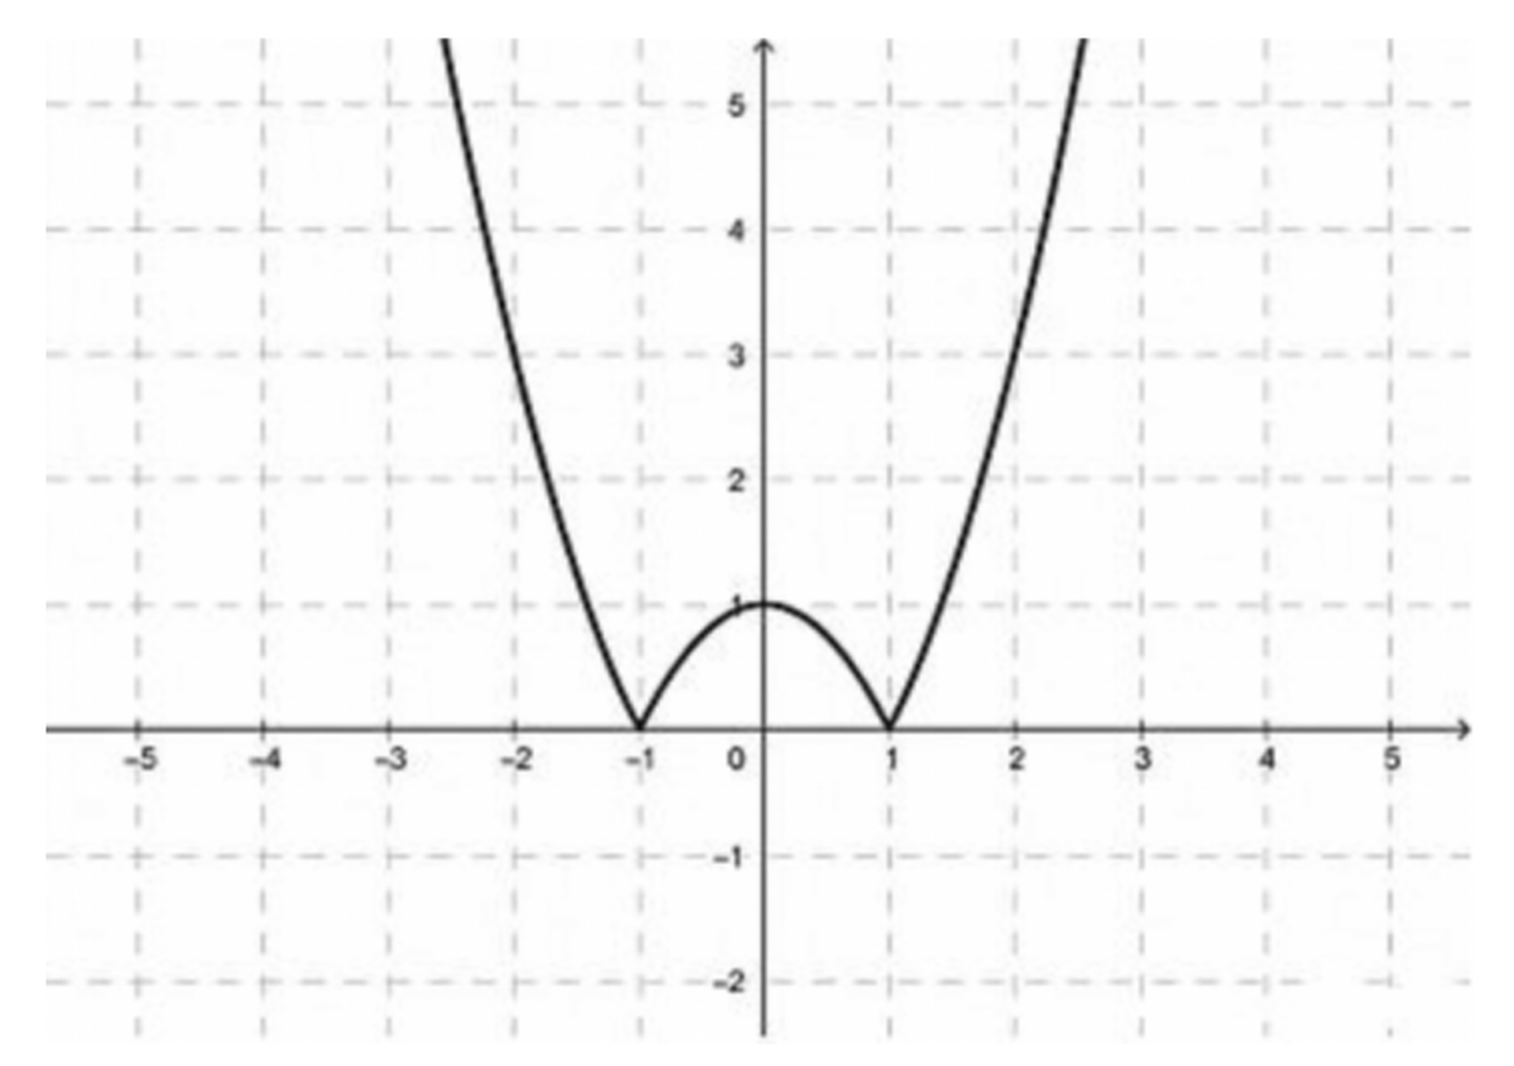
\includegraphics[width=0.55\textwidth]{figures/gao142_q21_para.png}
\end{center}}
\step{(3) 由题意得，$y_1=(2a)^2$，$y_2=(3-a)^2$，}
\step{$y_1<y_2$，即有 $(2a)^2<(3-a)^2$，化简整理得 $(a+3)(a-1)<0$，}
\step{解得实数 $a$ 的取值范围为 $(-3,1)$.}
\solend
\fi

\end{enumerate}

\end{document}
"
%
% ① 原始材料：微信公众号"魔都数学加油站"文章，连载"27学年高一142"，原文标题
% "27学年高一142——2026-2027年上海市群峰高级中学高一上期中"；
% 原文链接：https://mp.weixin.qq.com/s/cc7wnuP4Pk3OjNDV6ihB9A。
% 正文为 9 张 PNG 页（01、02、04、06、07、08、09 为 2560x3620；03、05 为 4762x6735，
% 同一篇各页分辨率不同，逐页按各自分辨率裁图核对），题目下印有【答案】或【解析】，为讲评版。
% 题目、解析均据原图转录；卷面粉红色水印"魔都数学加油站"及公众号页脚未录入。
% 全卷 4 幅插图：第 15 题四幅坐标函数图像选项（04 页，2x2 合并为一张）、
% 第 20 题矩形围栏示意图（07 页）、第 21 题 (2) 空白坐标网格（08 页）、
% 第 21 题抛物线图象（09 页，解析所附图）；均取原卷截图去粉色水印、LANCZOS 放大。
% 题目配图三版都出、解析配图仅答案版出。
%
% 卷首标题：原卷印作"2026-2027 年群峰高级中学高一上期中"（公众号标题中的"上海市"
% 卷面标题行没有，本稿照卷面），年份区间按全稿惯例排 en dash；原卷未印副标题，
% 本卷为期中卷、跨集合与常用逻辑用语／不等式／函数三章，按题目内容补出
% "集合与常用逻辑用语、不等式、函数"（头注说明，与同期中卷口径相同）。
%
% 题号体例：本卷共 19 题——一、填空题 3—12（10 题）、二、选择题 13—16（4 题）、
% 三、解答题 17—21（5 题）。三节分别 \setcounter{enumi}{2}／{12}／{16}。
% 原卷从第 3 题起、无第 1、2 题，本稿保留原题号。
%
% ② 与原卷的排版差异：
%   ① 原文从第 3 题起，本稿保留原题号；原卷未印副标题，本稿按"知识模块"口径补出；
%   ② 逐题答案口径：Q14 原卷把答案 D 印在题干括号内、且题目下无【解析】，本稿括号
%      留空 \mbox{（\quad）}、另提 \ans{D}；Q13／Q15／Q16 答案在【解析】末句"故选 …"
%      （分别为 C／C／A），题干括号留空、不另提 \ans{}；其余各题（Q3—Q12、
%      Q17—Q21）题目下印【解析】、答案融在解析中，不另提 \ans{}；全卷仅 Q14 一处 \ans{}；
%      答案版【答案】/【解析】标记数 = 19（1 个 \ans + 18 个 \solbegin）= 全卷题数；
%   ③ 原卷填空横线按全稿惯例排 \blankline[4.4em]；选择题括号排 \mbox{（\quad）}、
%      每个选项段前按惯例加 \keepwithprev（Q15 四幅图那一枚放在 \begin{center} 之前）；
%      解答题不留作答区、不加 \anspace（原卷为讲评版，与 129／131／132／133／136／140 同）；
%   ④ 原卷数集斜体 $R$（Q5、Q7、Q19、Q21 解析等）按全稿惯例统一改 \R；空集记号
%      \varnothing；绝对值排 \lvert…\rvert，集合描述竖线排 \mid；不等号按全稿惯例
%      排 \leqslant／\geqslant；
%   ⑤ 4 幅插图：Q15 四幅坐标函数图象选项合并裁为一张 \includegraphics（题前
%      \needvspace{9cm}）；Q15 是"二、选择题"节内带大图块的第 3 题（Q13、Q14 在前
%      且无图），另在 \bigsec{二、选择题} 之前加 \needvspace{11cm} 连节标题一起量
%      ——守卫必须放在 \bigsec 之前，放标题之后会让"二、选择题"孤立在页末
%      （B 类，照 高一26／40／59／136／140 成例）；Q20 围栏图与 Q21 网格图置于题干
%      之后（三版都出），Q21 抛物线图置于答案版解析 (2) 与 (3) 之间（仅答案版出）；
%   ⑥ 子题标号按原卷排半角 (1)(2)(3)（与 140／141 同期中卷口径相同）；括注全角／
%      半角逐处照录：Q3"（用含有 m 的代数式表示）"、Q6"（舍）"、Q10"（万元）"、
%      Q18"（请务必书写必要的计算步骤）"、Q20"（墙足够长）"印全角；Q15
%      "$y=a^x(a>0 且 a\neq1)$"、Q10"$y=x^a(a 为常数)$"、Q20"$t=\sqrt{xy}(t>0)$"
%      等数学式内括注印半角；数学式内 CJK 用 \text{…}（否则 FONTCHK 报缺字）；
%   ⑦ 数学式内半角逗号照录（如 Q6"$ax-1=0,a\in\R$"、Q9"$b=2+\sqrt2,a=\sqrt2+1$"、
%      Q16 区间 "$[-1,3]$"、Q21"$y_1<y_2$，即 $(2a)^2<(3-a)^2$" 等）；原卷行末
%      西文句点照录（Q7"(-3,5)."、Q10"125（万元）."、Q19 题干句点、Q20 题干
%      "矩形菜园."与"宽为 y 米."、Q21 题干"对称." 等）；行中全角逗号、分号照录；
%   ⑧ 题干中的中文弯引号：本卷题干与解析通篇未出现中文弯引号，故无此项；
%      圈数字 ①②③ 亦未出现（子题用 (1)(2)(3)）；
%   ⑨ 原卷"图像／图象"两种写法混用，逐处放大核对并照录：Q4 题干与解析作"图象"、
%      Q7 解析作"图象"、Q8 题干作"图像"而解析作"图象"、Q15 题干与解析通篇作
%      "图像"、Q21 题干与解析通篇作"图象"；
%   ⑩ 原卷无红色加粗标签（【解析】均黑色印刷；逐页扫描深红像素为 0），故本卷未用
%      \stepm；黑色常规分步标签（"A 中""C 中""D 中""(1)(2)(3)" 等）按普通 \step
%      行内文字照录；
%   ⑪ 跨页续印按题合并，明细见 ⑥。
%
% ③ 行数复核：一条 \step = 原卷解析的一个印刷行，cases 块作一个印刷行计。逐题数 \step
%   条数，合计 98 条（Q3：1；Q4：2；Q5：3；Q6：4；Q7：5；Q8：2；Q9：4；Q10：3；
%   Q11：4；Q12：3；Q13：5；Q14：0；Q15：10；Q16：4；Q17：10；Q18：3；
%   Q19：10；Q20：13；Q21：12），与原卷印刷行逐题相等。Q14 只把答案印在题干括号、
%   无【解析】，提 \ans{D}、不计入 \step 账；答案版标记数 = 19（1 个 \ans + 18 个
%   \solbegin）= 全卷题数。
%
% ④ 判别式字形：全卷判别式共 3 处——第 7 题【解析】"即判别式△<0"、
%   "即△=(a-1)^2-4×1×4<0" 两处原卷印扁等边三角 $\triangle$，
%   第 11 题【解析】cases 块"△=4a^2-4(a+6)≥0" 一处原卷印等腰偏高的高三角 $\Delta$；
%   逐处放大核对，两形不同、全卷混用，本稿逐处照录不统一（参照 高一141 头注④口径）。
%   子集符号：全卷共 3 处——第 6 题题干"若 B⊆A"、第 6 题【解析】"因为 B⊆A"、
%   第 17 题【解析】(2)"所以 A⊆B"，逐处放大核对，原卷三处均印带下划线的
%   $\subseteq$（不是单线 $\subset$），本稿一律照录 \subseteq；全卷未出现 \subset。
%
% ⑤ 原卷存疑照录（均照录未改，正文对应处另有 % 注）：
%   第 14 题题干括号内原卷印答案 D（非留空），且题目下无【解析】，按"答案印括号且
%      无解析"口径括号留空、另提 \ans{D}；
%   第 15 题【解析】"C 中，由指数函数 … 图像递减得 a>1" 中"递减"与"a>1"
%      自相矛盾（递减应得 0<a<1，疑为"递增"之误），照录；
%   第 16 题选项 B 作 $(-\infty,3]\cup[3,+\infty)$，两端区间并起即全体实数、
%      与正确答案 $[-1,3]$ 不成干扰项（疑为 $(-\infty,-1]\cup[3,+\infty)$ 之误），照录；
%   第 21 题 (2) 空白坐标网格的 x 轴刻度原卷印作"-5 -3 -3 -2 -1 0 1 2 3 4 5"
%      （"-3"重复，疑为"-4"之误），系插图中的印刷内容，取原卷截图照录、不改图。
%
% ⑥ 跨页续印说明：Q7 题干与解析首行在 01 页、解析续至 02 页；Q11 题干与解析
%   4 行在 03 页；Q13 解析前 4 行在 03 页、末句"故选 C."续至 04 页；Q15 题干与
%   四幅图在 04 页、解析前 8 行在 04 页、末 2 行续至 05 页；Q17 解析前 7 行在
%   05 页、后 3 行续至 06 页；Q19 解析前 5 行在 06 页、后 5 行续至 07 页；
%   Q20 解析前 9 行在 07 页、后 4 行续至 08 页；Q21 解析 (1)(2) 9 行在 08 页、
%   抛物线图与 (3) 3 行续至 09 页；本稿按题连排，不丢行。三版切页审计结论见
%   编译自验回报（切页守卫见 ②⑤）。
%
\documentclass[a4paper,11pt]{article}
\usepackage{common}

\begin{document}

\examtitlest[3]{2026--2027 年群峰高级中学高一上期中}{集合与常用逻辑用语、不等式、函数}

\bigsec{一、填空题}

\begin{enumerate}
\setcounter{enumi}{2}

\item 已知 $\log_2 3=m$，则 $\log_3 6=$\blankline[4.4em]（用含有 $m$ 的代数式表示）.

\ifanswer
\solbegin
\step{$\log_3 6=\dfrac{\log_2 6}{\log_2 3}=\dfrac{\log_2 2+\log_2 3}{\log_2 3}=\dfrac{1+m}{m}=\dfrac1m+1$.}
\solend
\fi

\item 若指数函数 $y=a^x$ 的图象经过点 $(3,27)$，则 $a$ 的值为\blankline[4.4em].

\ifanswer
\solbegin
\step{因为指数函数 $y=a^x$ 的图象经过点 $(3,27)$，}
\step{所以 $a^3=27=3^3$，所以 $a=3$.}
\solend
\fi

\item 不等式 $(2x+1)^{\frac13}<(3-x)^{\frac13}$ 的解集为\blankline[4.4em].

\ifanswer
\solbegin
\step{因为幂函数 $f(t)=t^{\frac13}$ 在 $\R$ 上严格增，}
\step{所以原不等式等价于 $2x+1<3-x$，解得 $x<\dfrac23$，}
\step{因此原不等式的解集为 $\left(-\infty,\dfrac23\right)$.}
\solend
\fi

\item 设集合 $A=\{1,-2\}$，$B=\{x\mid ax-1=0,a\in\R\}$，若 $B\subseteq A$，则 $a$ 的值为\blankline[4.4em].% 子集符号原卷印带下划线 $\subseteq$，照录

\ifanswer
\solbegin
\step{因为 $B\subseteq A$，所以 $B=\varnothing$ 或 $\{-2\}$ 或 $\{1\}$ 或 $\{1,-2\}$（舍），}% 子集符号原卷印带下划线 $\subseteq$，照录
\step{若 $B=\varnothing$，则 $a=0$；若 $B=\{1\}$，则 $a=1$；}
\step{若 $B=\{-2\}$，则 $-2a=1$，解得 $a=-\dfrac12$；}
\step{综上，$a=0$ 或 $1$ 或 $-\dfrac12$.}
\solend
\fi

\item 不等式 $x^2+(a-1)x+4>0$ 在 $\R$ 上恒成立，则实数 $a$ 的取值范围是\blankline[4.4em].

\ifanswer
\solbegin
\step{不等式 $x^2+(a-1)x+4>0$，对应的二次函数为 $y=x^2+(a-1)x+4$，}
\step{因此函数图象开口向上，要使不等式对任意实数 $x$ 恒成立，}
\step{需二次函数图象与 $x$ 轴无交点，即判别式 $\triangle<0$，}% 判别式原卷印扁等边三角 $\triangle$，照录
\step{即 $\triangle=(a-1)^2-4\times1\times4<0$，整理得 $a^2-2a-15<0$，}% 判别式原卷印扁等边三角 $\triangle$，照录
\step{解得 $-3<a<5$，故实数 $a$ 的取值范围是 $(-3,5)$.}
\solend
\fi

\item 函数 $f(x)=(5x-3)^a$ 的图像恒过点\blankline[4.4em].% 题干作"图像"、解析作"图象"，原卷混用，逐处照录

\ifanswer
\solbegin
\step{令 $5x-3=1$ 得 $x=\dfrac45$，此时 $f\left(\dfrac45\right)=\left(5\times\dfrac45-3\right)^a=1$，}
\step{所以 $f(x)$ 的图象恒过 $\left(\dfrac45,1\right)$.}
\solend
\fi

\item 若 $a>0$，$b>0$ 且 $\dfrac1a+\dfrac2b=1$，则 $a+b$ 的最小值为\blankline[4.4em].

\ifanswer
\solbegin
\step{因为 $a>0$，$b>0$，$\dfrac1a+\dfrac2b=1$，}
\step{所以 $a+b=(a+b)\left(\dfrac1a+\dfrac2b\right)=1+\dfrac{2a}{b}+\dfrac{b}{a}+2\geqslant3+2\sqrt{\dfrac{2a}{b}\cdot\dfrac{b}{a}}=3+2\sqrt2$，}
\step{当且仅当 $\dfrac{2a}{b}=\dfrac{b}{a}$，即 $b=2+\sqrt2,a=\sqrt2+1$ 时取等号，}
\step{故 $a+b$ 的最小值为 $3+2\sqrt2$.}
\solend
\fi

\item 某药厂研制出一种新型药剂，投放市场后其广告投入 $x$（万元）与药品利润 $y$（万元）存在的关系为 $y=x^a(a\text{ 为常数})$，其中 $x$ 不超过 5 万元. 已知去年投入广告费用为 3 万元时，药品利润为 27 万元，若今年投入广告费用 5 万元，预计今年药品利润为\blankline[4.4em]万元.

\ifanswer
\solbegin
\step{由已知投入广告费用为 3 万元时，药品利润为 27 万元，}
\step{代入 $y=x^a$ 中，即 $3^a=27$，解得 $a=3$，故函数关系式为 $y=x^3$，}
\step{所以当 $x=5$ 时，$y=125$（万元）.}
\solend
\fi

\item 已知方程 $x^2+2ax+a+6=0$ 的两根分别是 $x_1$ 和 $x_2$，且满足 $\dfrac1{x_1}+\dfrac1{x_2}<0$，则实数 $a$ 的取值范围是\blankline[4.4em].

\ifanswer
\solbegin
\step{由于方程 $x^2+2ax+a+6=0$ 的两根分别是 $x_1$ 和 $x_2$，}
\step{则 $\begin{cases}\Delta=4a^2-4(a+6)\geqslant0\\x_1+x_2=-2a\\x_1x_2=a+6\end{cases}$，解得 $a\geqslant3$ 或 $a\leqslant-2$.}% 判别式原卷印等腰偏高的高三角 $\Delta$，照录（与第 7 题扁等边 $\triangle$ 两形混用）
\step{又 $\dfrac1{x_1}+\dfrac1{x_2}<0$，即 $\dfrac{x_1+x_2}{x_1\cdot x_2}<0$，故 $\dfrac{-2a}{a+6}<0$，解得 $a<-6$ 或 $a>0$.}
\step{综上，$a$ 的取值范围是 $(-\infty,-6)\cup[3,+\infty)$.}
\solend
\fi

\item 已知 $b>a>1$，若 $\log_a b-\log_b a=\dfrac32$，$a^b=b^a$，则 $a-b=$\blankline[4.4em].

\ifanswer
\solbegin
\step{因为 $b>a>1$，所以 $\log_a b>1$，}
\step{由 $\log_a b-\log_b a=\log_a b-\dfrac{1}{\log_a b}=\dfrac32$，解得 $\log_a b=2$ 即 $b=a^2$，}
\step{因为 $a^b=b^a=a^{2a}$，所以 $b=2a=a^2$，所以 $a=2$，$b=4$，则 $a-b=-2$.}
\solend
\fi

\end{enumerate}

% 第 15 题四幅图是"二、选择题"节内的大图块；守卫须放在 \bigsec 之前连节标题一起量
\needvspace{11cm}
\bigsec{二、选择题}

\begin{enumerate}
\setcounter{enumi}{12}

\item 若 $a>b$，$c<0$，则下列不等式正确的是\mbox{（\quad）}

\keepwithprev
A. $ab>bc$\qquad B. $a+c<b+c$\qquad C. $ac^2>bc^2$\qquad D. $\dfrac ac>\dfrac bc$

\ifanswer
\solbegin
\step{因为 $a>b$，$c<0$，取 $b=0$，则 $ab=bc=0$，故 $A$ 错误；}
\step{由于 $a>b$，所以 $a+c>b+c$，故 $B$ 错误；}
\step{由 $c<0$ 得 $c^2>0$，所以 $ac^2>bc^2$，故 $C$ 正确；}
\step{由于 $a>b$ 且 $c<0$，所以 $\dfrac ac<\dfrac bc$，故 $D$ 错误.}
\step{故选 $C$.}
\solend
\fi

\item 若 $x>0$，$y>0$，则下列各式中，恒成立的是\mbox{（\quad）}% 原卷题干括号内印答案 D、且题目下无【解析】，本稿括号留空、另提 \ans{D}

\keepwithprev
A. $\lg x+\lg y=\lg(x+y)$\qquad B. $\lg x^2=(\lg x)^2$

C. $\dfrac{\lg x}{\lg y}=\lg(x-y)$\qquad D. $\lg x^{\frac1n}=\dfrac{\lg x}{n}$

\ifanswer
\ans{$D$}
\fi

% 第 15 题四幅坐标函数图象选项是一整块，守卫放在 \item 之前
\needvspace{9cm}
\item 在同一平面直角坐标系中，指数函数 $y=a^x(a>0\text{ 且 }a\neq1)$ 和一次函数 $y=a(x+1)$ 的图像关系可能是\mbox{（\quad）}

\keepwithprev
\begin{center}
% 四幅坐标函数图象选项取原卷 04 页截图去粉色水印、去色，按原卷 2x2 排布合并为一张
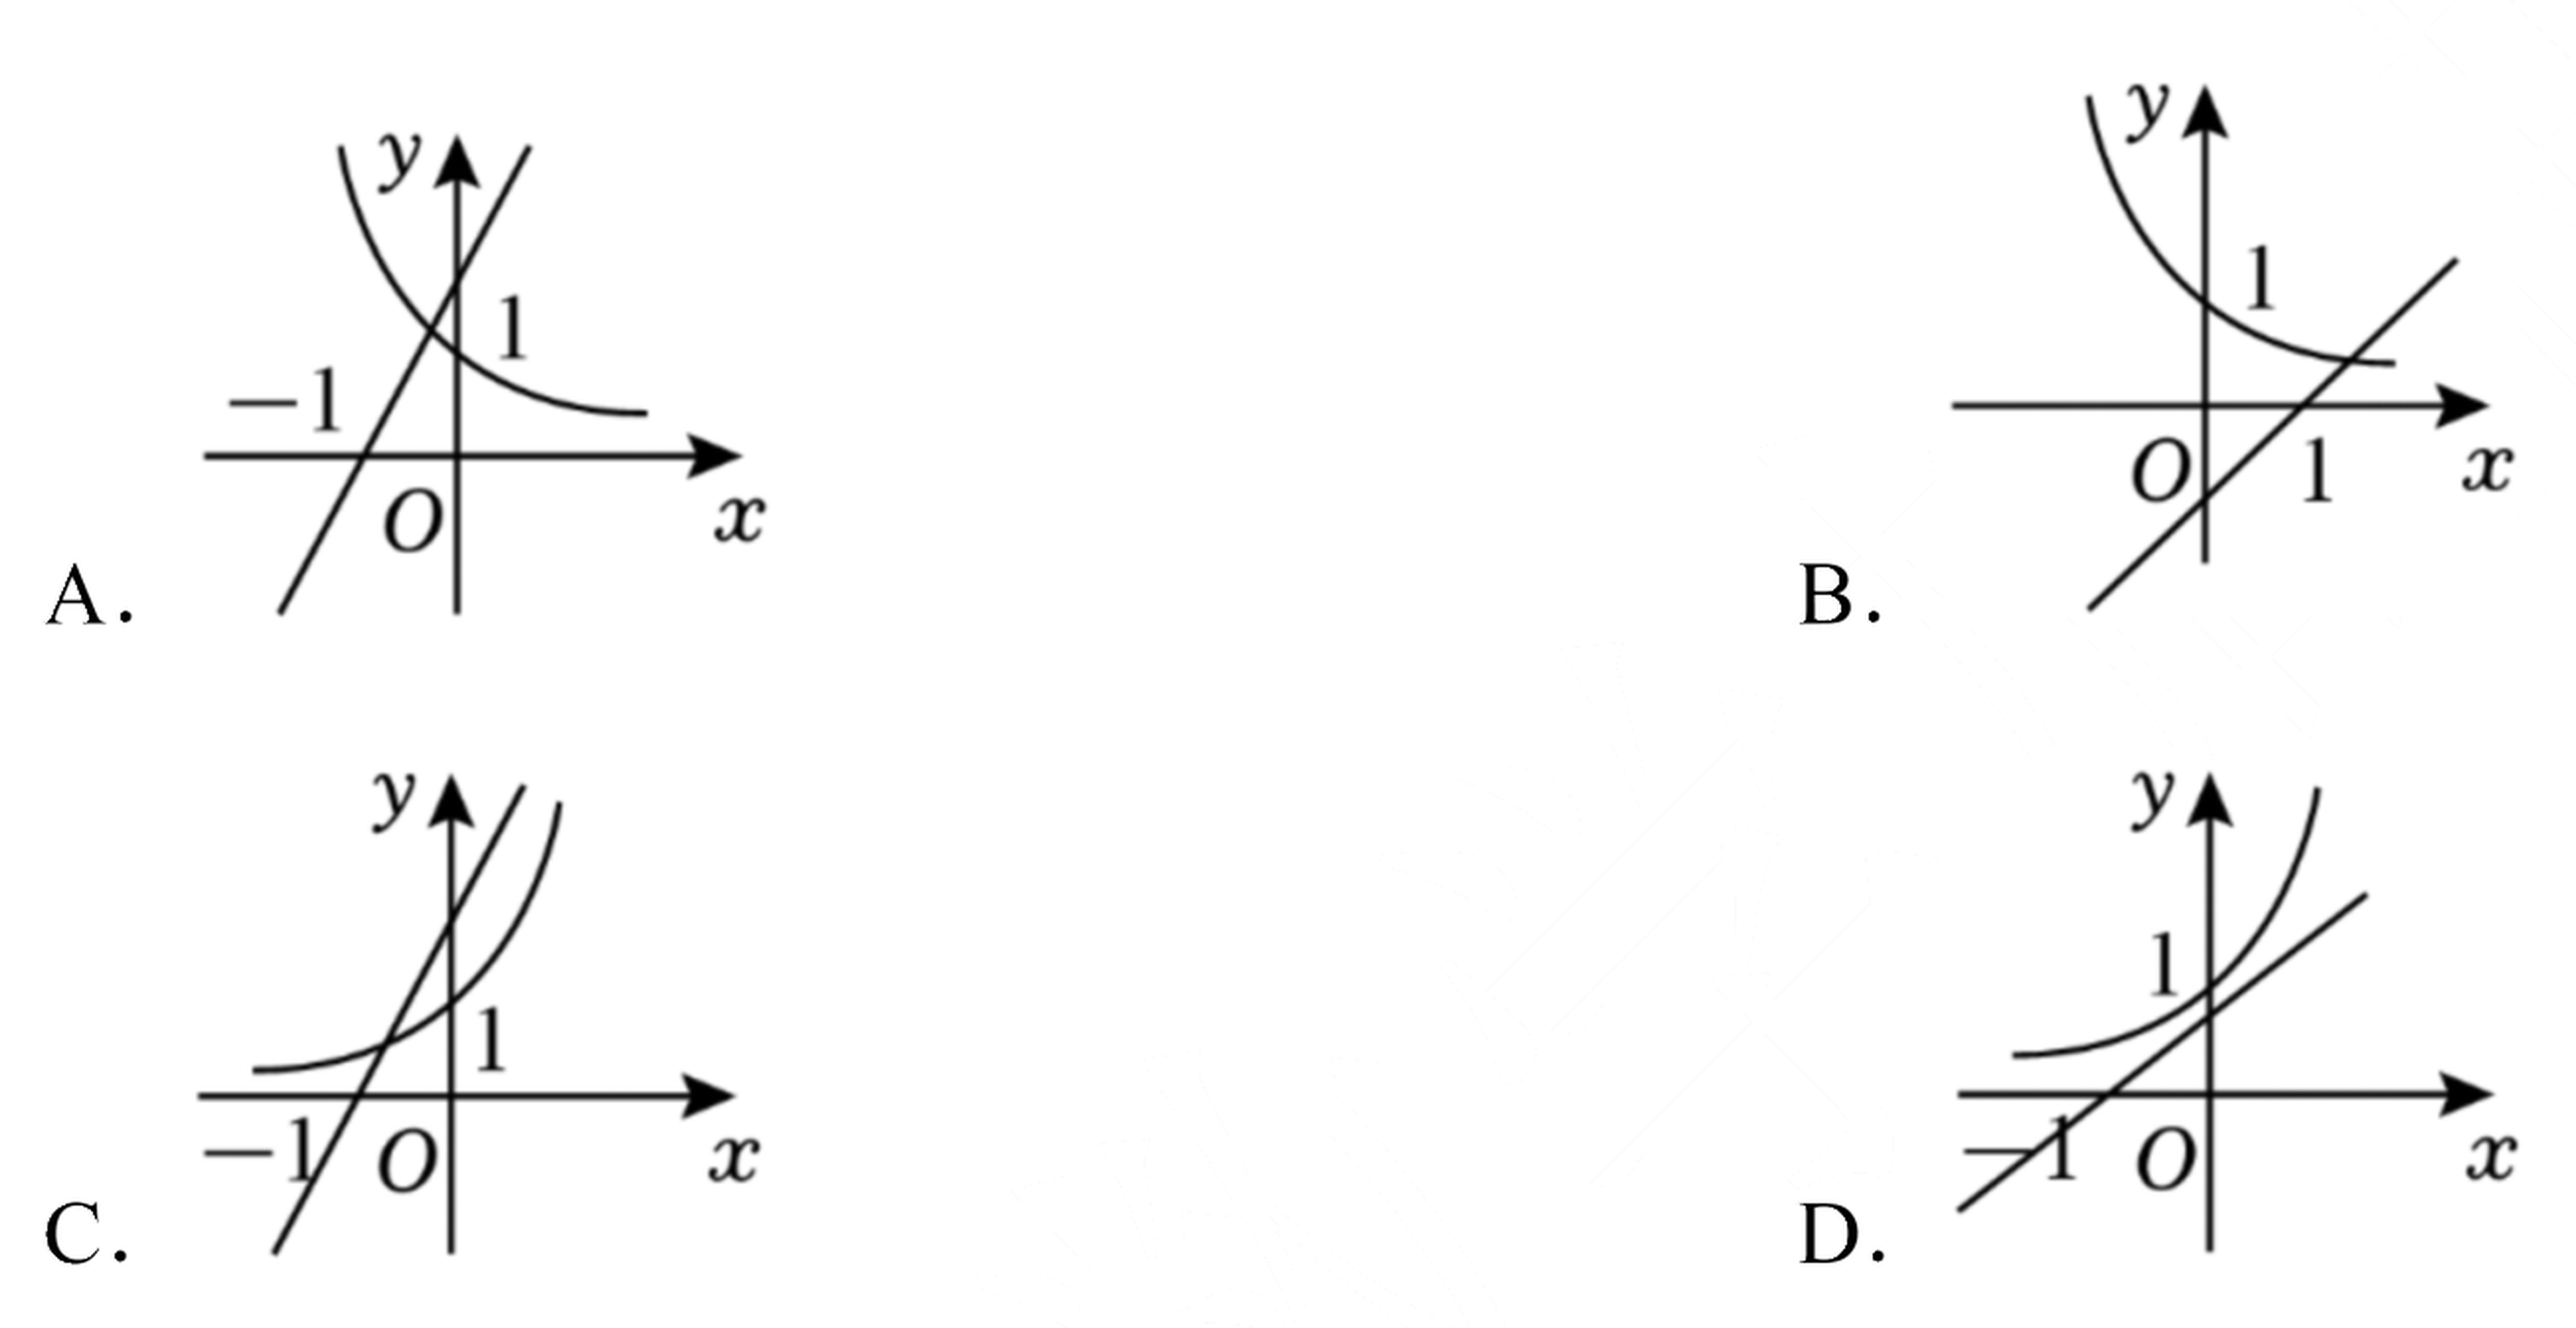
\includegraphics[width=0.80\textwidth]{figures/gao142_q15.png}
\end{center}

\ifanswer
\solbegin
\step{$A$ 中，由指数函数 $y=a^x(a>0\text{ 且 }a\neq1)$ 图像递减得 $0<a<1$，}
\step{而一次函数 $y=a(x+1)$ 的图像与 $y$ 轴交点纵坐标为 $a>1$，二者矛盾，}
\step{所以 $A$ 错；}
\step{由一次函数 $y=a(x+1)$ 的图像与 $x$ 轴交点横坐标为 $-1$，排除 $B$；}
\step{$C$ 中，由指数函数 $y=a^x(a>0\text{ 且 }a\neq1)$ 图像递减得 $a>1$，}% 原卷"递减得 a>1"自相矛盾（递减应得 0<a<1），照录
\step{而一次函数 $y=a(x+1)$ 的图像与 $y$ 轴交点纵坐标为 $a>1$，二者 $a$ 值吻合，}
\step{所以 $C$ 对；}
\step{$D$ 中，由一次函数 $y=a(x+1)$ 的图像得 $a=1$，与 $a>0$ 且 $a\neq1$ 矛盾，}
\step{所以 $D$ 错.}
\step{故选 $C$.}
\solend
\fi

\item 不等式 $\lvert x+1\rvert+\lvert 2-x\rvert\geqslant a^2-2a$ 恒成立，则 $a$ 的取值范围是\mbox{（\quad）}

\keepwithprev
A. $[-1,3]$\qquad B. $(-\infty,3]\cup[3,+\infty)$\qquad C. $(-\infty,3)$\qquad D. $(3,+\infty)$

\ifanswer
\solbegin
\step{因为 $\lvert x+1\rvert+\lvert 2-x\rvert\geqslant\lvert(x+1)+(2-x)\rvert=3$，}
\step{所以 $\lvert x+1\rvert+\lvert 2-x\rvert$ 的最小值为 3，}
\step{因为 $\lvert x+1\rvert+\lvert 2-x\rvert\geqslant a^2-2a$ 恒成立，所以只需 $a^2-2a\leqslant3$，所以 $-1\leqslant a\leqslant3$，}
\step{所以 $a$ 的取值范围为 $[-1,3]$. 故选 $A$.}
\solend
\fi

\end{enumerate}

\bigsec{三、解答题}

\begin{enumerate}
\setcounter{enumi}{16}

\item 已知集合 $A=\left\{x\mid\dfrac{x-3}{x-1}\leqslant0\right\}$，$B=\{x\mid\lvert x-1\rvert<a\}$.

(1) 若 $a=1$，求 $A\cap B$；

(2) 若 $x\in A$ 是 $x\in B$ 的充分条件，求 $a$ 的取值范围.

\ifanswer
\solbegin
\step{(1) 不等式 $\dfrac{x-3}{x-1}\leqslant0$，等价于 $(x-3)(x-1)\leqslant0$ 且 $x-1\neq0$，解得 $1<x\leqslant3$，}
\step{所以 $A=\{x\mid 1<x\leqslant3\}$，}
\step{当 $a=1$ 时，不等式 $\lvert x-1\rvert<a$ 可化为 $\lvert x-1\rvert<1$，所以 $-1<x-1<1$，}
\step{故 $0<x<2$，所以 $B=\{x\mid 0<x<2\}$，}
\step{所以 $A\cap B=\{x\mid 1<x<2\}$；}
\step{(2) 因为 $x\in A$ 是 $x\in B$ 的充分条件，所以 $A\subseteq B$，}% 子集符号原卷印带下划线 $\subseteq$，照录
\step{因为 $A=\{x\mid 1<x\leqslant3\}\neq\varnothing$，所以 $B\neq\varnothing$，故 $a>0$，}
\step{由不等式 $\lvert x-1\rvert<a$，解得 $1-a<x<1+a$，}
\step{所以 $B=\{x\mid 1-a<x<1+a\}$，所以 $\begin{cases}1-a\leqslant1\\1+a>3\end{cases}$，解得 $a>2$，}
\step{所以 $a$ 的取值范围为 $(2,+\infty)$.}
\solend
\fi

\item 计算下列式子的值（请务必书写必要的计算步骤）

(1) $27^{\frac13}+\left(\dfrac76\right)^0+\sqrt{(3-\pi)^2}$；

(2) $\lg25+\lg4+7^{\log_7 2}-\log_2 3\times\log_3 4+\log_3 9$.

\ifanswer
\solbegin
\step{(1) $27^{\frac13}+\left(\dfrac76\right)^0+\sqrt{(3-\pi)^2}=3^{3\times\frac13}+1+\lvert 3-\pi\rvert=3+1+\pi-3=\pi+1$；}
\step{(2) 原式 $=\lg(25\times4)+2-\dfrac{\lg3}{\lg2}\times\dfrac{\lg4}{\lg3}+2=\lg100+2-\dfrac{2\lg2}{\lg2}+2$}
\step{$=2+2-2+2=4$.}
\solend
\fi

\item 已知关于 $x$ 的不等式 $mx^2-(3m^2-m+2)x+6m-2\geqslant0$.

(1) 当 $m=2$ 时，求关于 $x$ 的不等式的解集；

(2) 当 $m>0$ 时，求关于 $x$ 的不等式的解集.

\ifanswer
\solbegin
\step{(1) $m=2$ 时，不等式为 $x^2-6x+5\geqslant0$，即 $(x-1)(x-5)\geqslant0$，}
\step{解得 $x\leqslant1$ 或 $x\geqslant5$，所以不等式的解集是 $\{x\mid x\leqslant1$ 或 $x\geqslant5\}$.}
\step{(2) $m>0$ 时，不等式可化为 $(mx-2)[x-(3m-1)]\geqslant0$，}
\step{即 $\left(x-\dfrac2m\right)[x-(3m-1)]\geqslant0$，}
\step{若 $m=1$，则不等式为 $(x-2)^2\geqslant0$，解得 $x\in\R$；}
\step{若 $0<m<1$，则 $\dfrac2m>3m-1$，解不等式得 $x\geqslant\dfrac2m$ 或 $x\leqslant3m-1$；}
\step{若 $m>1$，则 $\dfrac2m<3m-1$，解不等式得 $x\geqslant3m-1$ 或 $x\leqslant\dfrac2m$；}
\step{综上，$0<m<1$ 时，不等式的解集是 $\{x\mid x\leqslant3m-1$ 或 $x\geqslant\dfrac2m\}$；}
\step{$m=1$ 时，不等式的解集为 $\R$；}
\step{$m>1$ 时，不等式的解集是 $\{x\mid x\leqslant\dfrac2m$ 或 $x\geqslant3m-1\}$.}
\solend
\fi

\item 如图，某人计划用篱笆围成一个一边靠墙（墙足够长）的矩形菜园. 设菜园的长为 $x$ 米，宽为 $y$ 米.

\begin{center}
% 矩形围栏示意图取原卷 07 页截图去粉色水印、去色、LANCZOS 放大；题目配图，三版都出
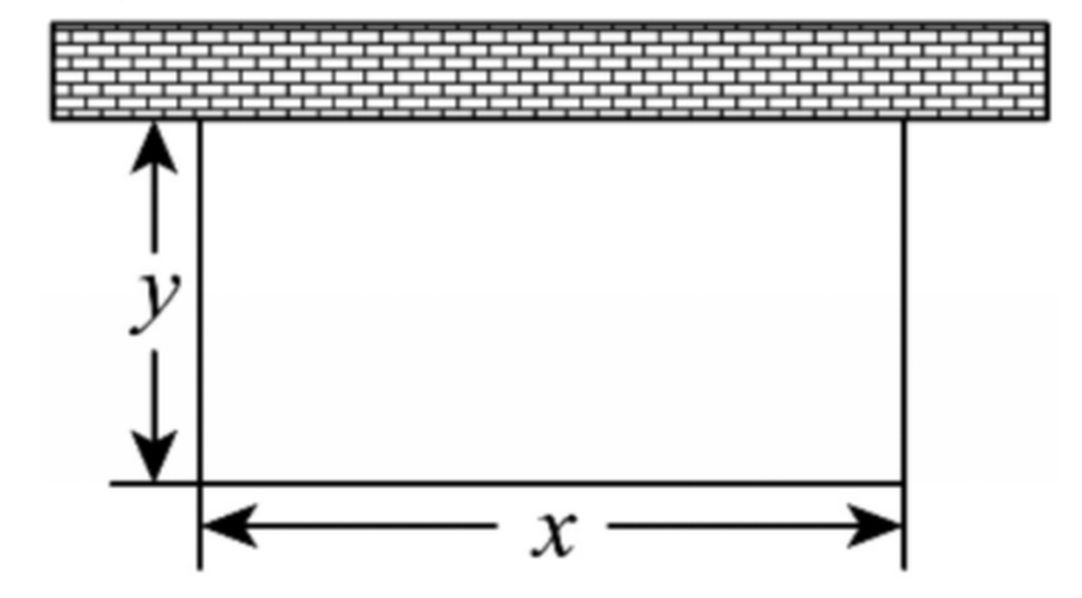
\includegraphics[width=0.42\textwidth]{figures/gao142_q20.png}
\end{center}

(1) 若菜园面积为 72 平方米，则 $x$、$y$ 为何值时，所用篱笆总长最小？

(2) 若 $x$、$y$ 满足 $x+y-xy+63=0$，则菜园面积最小为多少平方米？

\ifanswer
\solbegin
\step{(1) 由题意得，菜园的面积 $S=xy=72$，且 $x>0$，$y>0$，}
\step{所用篱笆总长 $L=x+2y$，}
\step{由基本不等式得 $x+2y\geqslant2\sqrt{x\cdot2y}=2\sqrt{2xy}=2\sqrt{2\times72}=24$，}
\step{当且仅当 $x=2y$ 时取等号，}
\step{联立 $\begin{cases}xy=72\\x=2y\end{cases}$，解得 $\begin{cases}x=12\\y=6\end{cases}$，}
\step{所以当 $x=12$，$y=6$ 时，所用篱笆总长最小；}
\step{(2) 由题意得 $x>0$，$y>0$，且满足 $x+y-xy+63=0$，即 $x+y=xy-63$，}
\step{由基本不等式得 $x+y\geqslant2\sqrt{xy}$，当且仅当 $x=y$ 时取等号，}
\step{所以 $xy-63\geqslant2\sqrt{xy}$. 令 $t=\sqrt{xy}(t>0)$，则 $xy=t^2$，}
\step{上述不等式可化为 $t^2-2t-63\geqslant0$，即 $(t-9)(t+7)\geqslant0$，}
\step{因为 $t>0$，所以 $t+7>0$，故 $t-9\geqslant0$，解得 $t\geqslant9$，所以 $\sqrt{xy}\geqslant9$，}
\step{即 $xy\geqslant81$，当且仅当 $x=y=9$ 时取等号，此时满足 $9+9-81+63=0$，}
\step{所以菜园面积最小为 81 平方米.}
\solend
\fi

\item 已知幂函数 $f(x)=(m^2-3m+3)x^m$ 的图象关于 $y$ 轴对称.

(1) 求实数 $m$ 的值；

(2) 在平面直角坐标系中作出函数 $y=\lvert f(x)-1\rvert$ 的图象；

(3) 已知点 $A(2a,y_1)$ 与点 $B(3-a,y_2)$ 都在幂函数 $y=x^2$ 的图象上. 若 $y_1<y_2$，求实数 $a$ 的取值范围.

\begin{center}
% 空白坐标网格取原卷 08 页截图去粉色水印、去色、LANCZOS 放大；题目配图，三版都出
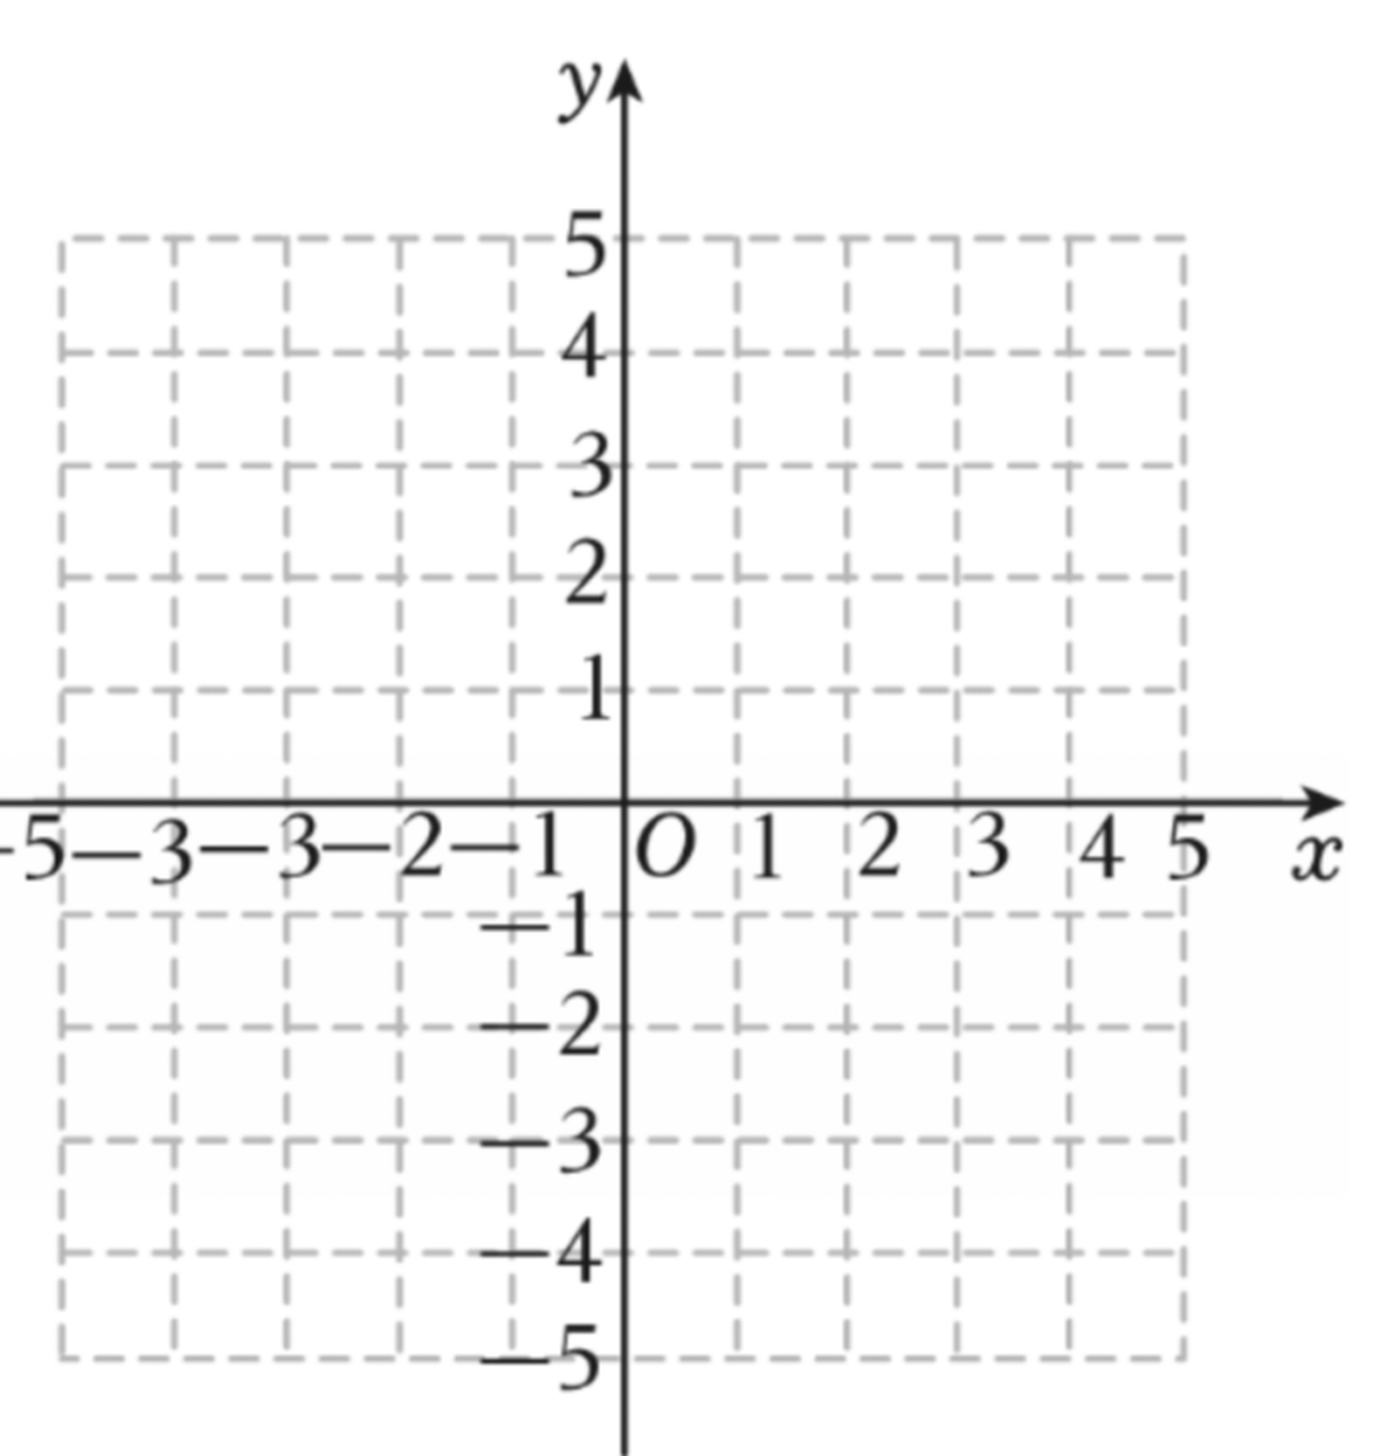
\includegraphics[width=0.52\textwidth]{figures/gao142_q21_grid.png}
\end{center}

\ifanswer
\solbegin
\step{(1) 由题意幂函数 $f(x)=(m^2-3m+3)x^m$，}
\step{故 $m^2-3m+3=1$，解得 $m=1$ 或 $m=2$，}
\step{又 $f(x)$ 图象关于 $y$ 轴对称，即 $f(x)$ 是偶函数，}
\step{当 $m=1$ 时，$f(x)=x$ 是奇函数，不满足条件，舍去；}
\step{当 $m=2$ 时，$f(x)=x^2$ 是偶函数，满足条件，故 $m=2$；}
\step{(2) 由 (1) 得，$\lvert f(x)-1\rvert=\lvert x^2-1\rvert$，}
\step{先画 $y=x^2-1$，开口向上的抛物线，顶点 $(0,-1)$，零点 $x=\pm1$，}
\step{再将 $x$ 轴下方的部分沿 $x$ 轴翻折到上方即为 $y=\lvert x^2-1\rvert$ 的图象，}
\step{图象如图所示.}
\par{\leftskip=0pt
\begin{center}
% 抛物线图象取原卷 09 页截图去粉色水印、去色、LANCZOS 放大；解析所附配图，仅答案版出
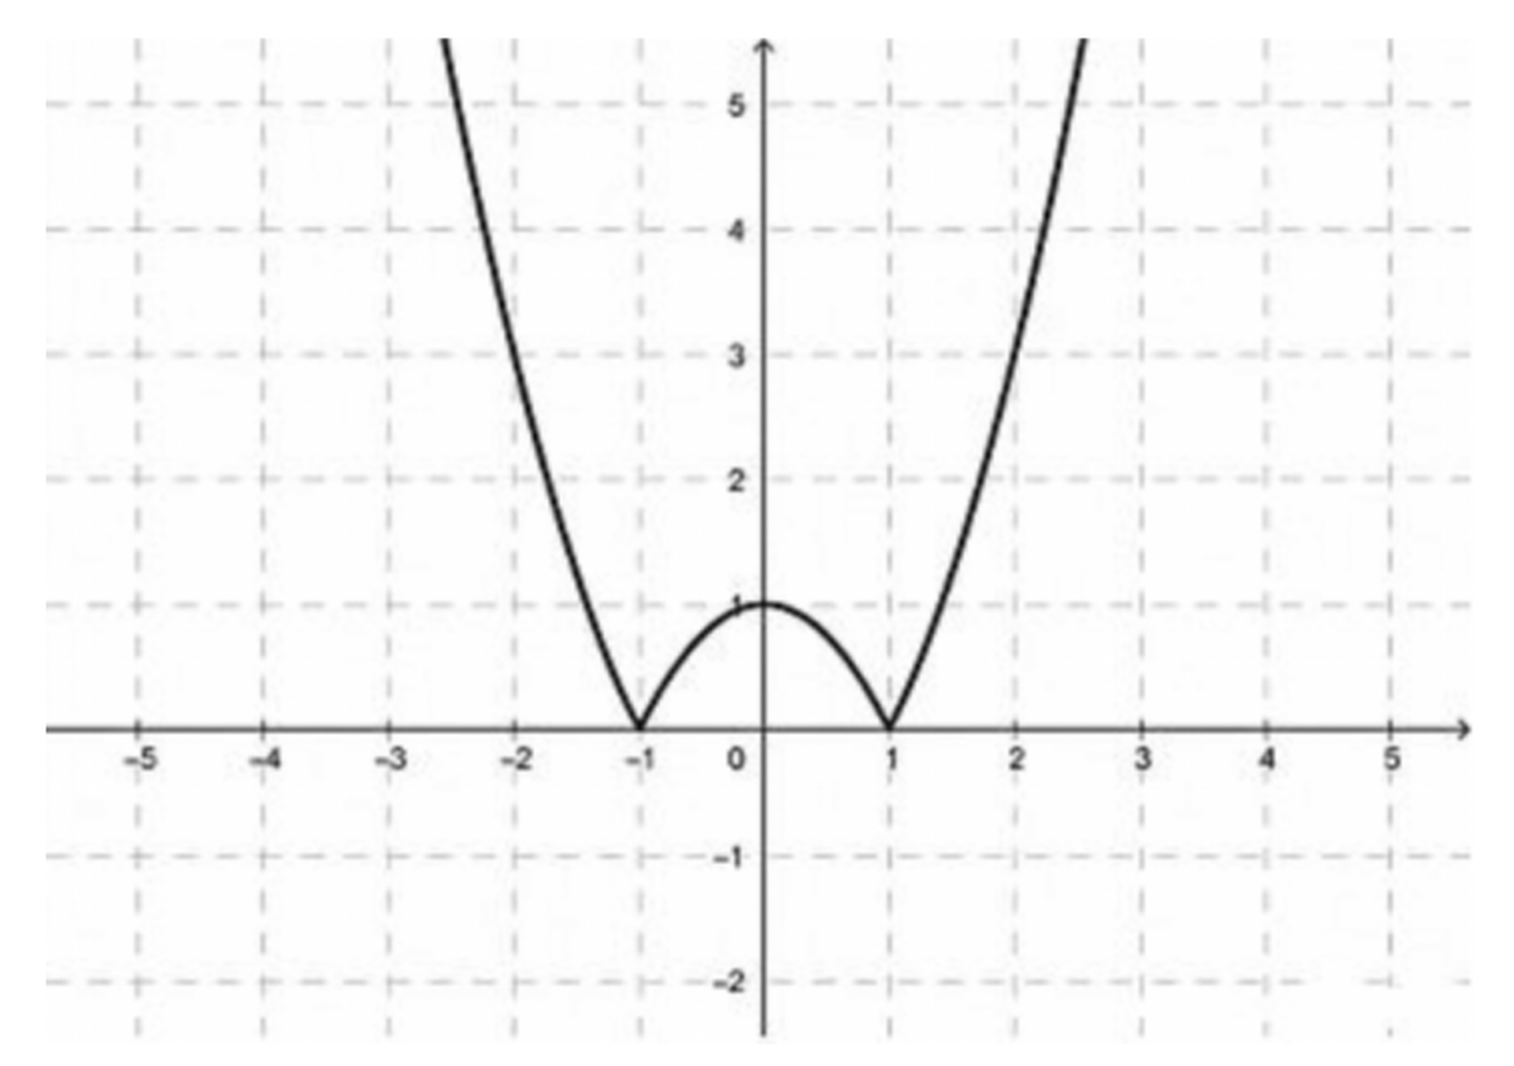
\includegraphics[width=0.55\textwidth]{figures/gao142_q21_para.png}
\end{center}}
\step{(3) 由题意得，$y_1=(2a)^2$，$y_2=(3-a)^2$，}
\step{$y_1<y_2$，即有 $(2a)^2<(3-a)^2$，化简整理得 $(a+3)(a-1)<0$，}
\step{解得实数 $a$ 的取值范围为 $(-3,1)$.}
\solend
\fi

\end{enumerate}

\end{document}
"
%
% ① 原始材料：微信公众号"魔都数学加油站"文章，连载"27学年高一142"，原文标题
% "27学年高一142——2026-2027年上海市群峰高级中学高一上期中"；
% 原文链接：https://mp.weixin.qq.com/s/cc7wnuP4Pk3OjNDV6ihB9A。
% 正文为 9 张 PNG 页（01、02、04、06、07、08、09 为 2560x3620；03、05 为 4762x6735，
% 同一篇各页分辨率不同，逐页按各自分辨率裁图核对），题目下印有【答案】或【解析】，为讲评版。
% 题目、解析均据原图转录；卷面粉红色水印"魔都数学加油站"及公众号页脚未录入。
% 全卷 4 幅插图：第 15 题四幅坐标函数图像选项（04 页，2x2 合并为一张）、
% 第 20 题矩形围栏示意图（07 页）、第 21 题 (2) 空白坐标网格（08 页）、
% 第 21 题抛物线图象（09 页，解析所附图）；均取原卷截图去粉色水印、LANCZOS 放大。
% 题目配图三版都出、解析配图仅答案版出。
%
% 卷首标题：原卷印作"2026-2027 年群峰高级中学高一上期中"（公众号标题中的"上海市"
% 卷面标题行没有，本稿照卷面），年份区间按全稿惯例排 en dash；原卷未印副标题，
% 本卷为期中卷、跨集合与常用逻辑用语／不等式／函数三章，按题目内容补出
% "集合与常用逻辑用语、不等式、函数"（头注说明，与同期中卷口径相同）。
%
% 题号体例：本卷共 19 题——一、填空题 3—12（10 题）、二、选择题 13—16（4 题）、
% 三、解答题 17—21（5 题）。三节分别 \setcounter{enumi}{2}／{12}／{16}。
% 原卷从第 3 题起、无第 1、2 题，本稿保留原题号。
%
% ② 与原卷的排版差异：
%   ① 原文从第 3 题起，本稿保留原题号；原卷未印副标题，本稿按"知识模块"口径补出；
%   ② 逐题答案口径：Q14 原卷把答案 D 印在题干括号内、且题目下无【解析】，本稿括号
%      留空 \mbox{（\quad）}、另提 \ans{D}；Q13／Q15／Q16 答案在【解析】末句"故选 …"
%      （分别为 C／C／A），题干括号留空、不另提 \ans{}；其余各题（Q3—Q12、
%      Q17—Q21）题目下印【解析】、答案融在解析中，不另提 \ans{}；全卷仅 Q14 一处 \ans{}；
%      答案版【答案】/【解析】标记数 = 19（1 个 \ans + 18 个 \solbegin）= 全卷题数；
%   ③ 原卷填空横线按全稿惯例排 \blankline[4.4em]；选择题括号排 \mbox{（\quad）}、
%      每个选项段前按惯例加 \keepwithprev（Q15 四幅图那一枚放在 \begin{center} 之前）；
%      解答题不留作答区、不加 \anspace（原卷为讲评版，与 129／131／132／133／136／140 同）；
%   ④ 原卷数集斜体 $R$（Q5、Q7、Q19、Q21 解析等）按全稿惯例统一改 \R；空集记号
%      \varnothing；绝对值排 \lvert…\rvert，集合描述竖线排 \mid；不等号按全稿惯例
%      排 \leqslant／\geqslant；
%   ⑤ 4 幅插图：Q15 四幅坐标函数图象选项合并裁为一张 \includegraphics（题前
%      \needvspace{9cm}）；Q15 是"二、选择题"节内带大图块的第 3 题（Q13、Q14 在前
%      且无图），另在 \bigsec{二、选择题} 之前加 \needvspace{11cm} 连节标题一起量
%      ——守卫必须放在 \bigsec 之前，放标题之后会让"二、选择题"孤立在页末
%      （B 类，照 高一26／40／59／136／140 成例）；Q20 围栏图与 Q21 网格图置于题干
%      之后（三版都出），Q21 抛物线图置于答案版解析 (2) 与 (3) 之间（仅答案版出）；
%   ⑥ 子题标号按原卷排半角 (1)(2)(3)（与 140／141 同期中卷口径相同）；括注全角／
%      半角逐处照录：Q3"（用含有 m 的代数式表示）"、Q6"（舍）"、Q10"（万元）"、
%      Q18"（请务必书写必要的计算步骤）"、Q20"（墙足够长）"印全角；Q15
%      "$y=a^x(a>0 且 a\neq1)$"、Q10"$y=x^a(a 为常数)$"、Q20"$t=\sqrt{xy}(t>0)$"
%      等数学式内括注印半角；数学式内 CJK 用 \text{…}（否则 FONTCHK 报缺字）；
%   ⑦ 数学式内半角逗号照录（如 Q6"$ax-1=0,a\in\R$"、Q9"$b=2+\sqrt2,a=\sqrt2+1$"、
%      Q16 区间 "$[-1,3]$"、Q21"$y_1<y_2$，即 $(2a)^2<(3-a)^2$" 等）；原卷行末
%      西文句点照录（Q7"(-3,5)."、Q10"125（万元）."、Q19 题干句点、Q20 题干
%      "矩形菜园."与"宽为 y 米."、Q21 题干"对称." 等）；行中全角逗号、分号照录；
%   ⑧ 题干中的中文弯引号：本卷题干与解析通篇未出现中文弯引号，故无此项；
%      圈数字 ①②③ 亦未出现（子题用 (1)(2)(3)）；
%   ⑨ 原卷"图像／图象"两种写法混用，逐处放大核对并照录：Q4 题干与解析作"图象"、
%      Q7 解析作"图象"、Q8 题干作"图像"而解析作"图象"、Q15 题干与解析通篇作
%      "图像"、Q21 题干与解析通篇作"图象"；
%   ⑩ 原卷无红色加粗标签（【解析】均黑色印刷；逐页扫描深红像素为 0），故本卷未用
%      \stepm；黑色常规分步标签（"A 中""C 中""D 中""(1)(2)(3)" 等）按普通 \step
%      行内文字照录；
%   ⑪ 跨页续印按题合并，明细见 ⑥。
%
% ③ 行数复核：一条 \step = 原卷解析的一个印刷行，cases 块作一个印刷行计。逐题数 \step
%   条数，合计 98 条（Q3：1；Q4：2；Q5：3；Q6：4；Q7：5；Q8：2；Q9：4；Q10：3；
%   Q11：4；Q12：3；Q13：5；Q14：0；Q15：10；Q16：4；Q17：10；Q18：3；
%   Q19：10；Q20：13；Q21：12），与原卷印刷行逐题相等。Q14 只把答案印在题干括号、
%   无【解析】，提 \ans{D}、不计入 \step 账；答案版标记数 = 19（1 个 \ans + 18 个
%   \solbegin）= 全卷题数。
%
% ④ 判别式字形：全卷判别式共 3 处——第 7 题【解析】"即判别式△<0"、
%   "即△=(a-1)^2-4×1×4<0" 两处原卷印扁等边三角 $\triangle$，
%   第 11 题【解析】cases 块"△=4a^2-4(a+6)≥0" 一处原卷印等腰偏高的高三角 $\Delta$；
%   逐处放大核对，两形不同、全卷混用，本稿逐处照录不统一（参照 高一141 头注④口径）。
%   子集符号：全卷共 3 处——第 6 题题干"若 B⊆A"、第 6 题【解析】"因为 B⊆A"、
%   第 17 题【解析】(2)"所以 A⊆B"，逐处放大核对，原卷三处均印带下划线的
%   $\subseteq$（不是单线 $\subset$），本稿一律照录 \subseteq；全卷未出现 \subset。
%
% ⑤ 原卷存疑照录（均照录未改，正文对应处另有 % 注）：
%   第 14 题题干括号内原卷印答案 D（非留空），且题目下无【解析】，按"答案印括号且
%      无解析"口径括号留空、另提 \ans{D}；
%   第 15 题【解析】"C 中，由指数函数 … 图像递减得 a>1" 中"递减"与"a>1"
%      自相矛盾（递减应得 0<a<1，疑为"递增"之误），照录；
%   第 16 题选项 B 作 $(-\infty,3]\cup[3,+\infty)$，两端区间并起即全体实数、
%      与正确答案 $[-1,3]$ 不成干扰项（疑为 $(-\infty,-1]\cup[3,+\infty)$ 之误），照录；
%   第 21 题 (2) 空白坐标网格的 x 轴刻度原卷印作"-5 -3 -3 -2 -1 0 1 2 3 4 5"
%      （"-3"重复，疑为"-4"之误），系插图中的印刷内容，取原卷截图照录、不改图。
%
% ⑥ 跨页续印说明：Q7 题干与解析首行在 01 页、解析续至 02 页；Q11 题干与解析
%   4 行在 03 页；Q13 解析前 4 行在 03 页、末句"故选 C."续至 04 页；Q15 题干与
%   四幅图在 04 页、解析前 8 行在 04 页、末 2 行续至 05 页；Q17 解析前 7 行在
%   05 页、后 3 行续至 06 页；Q19 解析前 5 行在 06 页、后 5 行续至 07 页；
%   Q20 解析前 9 行在 07 页、后 4 行续至 08 页；Q21 解析 (1)(2) 9 行在 08 页、
%   抛物线图与 (3) 3 行续至 09 页；本稿按题连排，不丢行。三版切页审计结论见
%   编译自验回报（切页守卫见 ②⑤）。
%
\documentclass[a4paper,11pt]{article}
\usepackage{common}

\begin{document}

\examtitlest[3]{2026--2027 年群峰高级中学高一上期中}{集合与常用逻辑用语、不等式、函数}

\bigsec{一、填空题}

\begin{enumerate}
\setcounter{enumi}{2}

\item 已知 $\log_2 3=m$，则 $\log_3 6=$\blankline[4.4em]（用含有 $m$ 的代数式表示）.

\ifanswer
\solbegin
\step{$\log_3 6=\dfrac{\log_2 6}{\log_2 3}=\dfrac{\log_2 2+\log_2 3}{\log_2 3}=\dfrac{1+m}{m}=\dfrac1m+1$.}
\solend
\fi

\item 若指数函数 $y=a^x$ 的图象经过点 $(3,27)$，则 $a$ 的值为\blankline[4.4em].

\ifanswer
\solbegin
\step{因为指数函数 $y=a^x$ 的图象经过点 $(3,27)$，}
\step{所以 $a^3=27=3^3$，所以 $a=3$.}
\solend
\fi

\item 不等式 $(2x+1)^{\frac13}<(3-x)^{\frac13}$ 的解集为\blankline[4.4em].

\ifanswer
\solbegin
\step{因为幂函数 $f(t)=t^{\frac13}$ 在 $\R$ 上严格增，}
\step{所以原不等式等价于 $2x+1<3-x$，解得 $x<\dfrac23$，}
\step{因此原不等式的解集为 $\left(-\infty,\dfrac23\right)$.}
\solend
\fi

\item 设集合 $A=\{1,-2\}$，$B=\{x\mid ax-1=0,a\in\R\}$，若 $B\subseteq A$，则 $a$ 的值为\blankline[4.4em].% 子集符号原卷印带下划线 $\subseteq$，照录

\ifanswer
\solbegin
\step{因为 $B\subseteq A$，所以 $B=\varnothing$ 或 $\{-2\}$ 或 $\{1\}$ 或 $\{1,-2\}$（舍），}% 子集符号原卷印带下划线 $\subseteq$，照录
\step{若 $B=\varnothing$，则 $a=0$；若 $B=\{1\}$，则 $a=1$；}
\step{若 $B=\{-2\}$，则 $-2a=1$，解得 $a=-\dfrac12$；}
\step{综上，$a=0$ 或 $1$ 或 $-\dfrac12$.}
\solend
\fi

\item 不等式 $x^2+(a-1)x+4>0$ 在 $\R$ 上恒成立，则实数 $a$ 的取值范围是\blankline[4.4em].

\ifanswer
\solbegin
\step{不等式 $x^2+(a-1)x+4>0$，对应的二次函数为 $y=x^2+(a-1)x+4$，}
\step{因此函数图象开口向上，要使不等式对任意实数 $x$ 恒成立，}
\step{需二次函数图象与 $x$ 轴无交点，即判别式 $\triangle<0$，}% 判别式原卷印扁等边三角 $\triangle$，照录
\step{即 $\triangle=(a-1)^2-4\times1\times4<0$，整理得 $a^2-2a-15<0$，}% 判别式原卷印扁等边三角 $\triangle$，照录
\step{解得 $-3<a<5$，故实数 $a$ 的取值范围是 $(-3,5)$.}
\solend
\fi

\item 函数 $f(x)=(5x-3)^a$ 的图像恒过点\blankline[4.4em].% 题干作"图像"、解析作"图象"，原卷混用，逐处照录

\ifanswer
\solbegin
\step{令 $5x-3=1$ 得 $x=\dfrac45$，此时 $f\left(\dfrac45\right)=\left(5\times\dfrac45-3\right)^a=1$，}
\step{所以 $f(x)$ 的图象恒过 $\left(\dfrac45,1\right)$.}
\solend
\fi

\item 若 $a>0$，$b>0$ 且 $\dfrac1a+\dfrac2b=1$，则 $a+b$ 的最小值为\blankline[4.4em].

\ifanswer
\solbegin
\step{因为 $a>0$，$b>0$，$\dfrac1a+\dfrac2b=1$，}
\step{所以 $a+b=(a+b)\left(\dfrac1a+\dfrac2b\right)=1+\dfrac{2a}{b}+\dfrac{b}{a}+2\geqslant3+2\sqrt{\dfrac{2a}{b}\cdot\dfrac{b}{a}}=3+2\sqrt2$，}
\step{当且仅当 $\dfrac{2a}{b}=\dfrac{b}{a}$，即 $b=2+\sqrt2,a=\sqrt2+1$ 时取等号，}
\step{故 $a+b$ 的最小值为 $3+2\sqrt2$.}
\solend
\fi

\item 某药厂研制出一种新型药剂，投放市场后其广告投入 $x$（万元）与药品利润 $y$（万元）存在的关系为 $y=x^a(a\text{ 为常数})$，其中 $x$ 不超过 5 万元. 已知去年投入广告费用为 3 万元时，药品利润为 27 万元，若今年投入广告费用 5 万元，预计今年药品利润为\blankline[4.4em]万元.

\ifanswer
\solbegin
\step{由已知投入广告费用为 3 万元时，药品利润为 27 万元，}
\step{代入 $y=x^a$ 中，即 $3^a=27$，解得 $a=3$，故函数关系式为 $y=x^3$，}
\step{所以当 $x=5$ 时，$y=125$（万元）.}
\solend
\fi

\item 已知方程 $x^2+2ax+a+6=0$ 的两根分别是 $x_1$ 和 $x_2$，且满足 $\dfrac1{x_1}+\dfrac1{x_2}<0$，则实数 $a$ 的取值范围是\blankline[4.4em].

\ifanswer
\solbegin
\step{由于方程 $x^2+2ax+a+6=0$ 的两根分别是 $x_1$ 和 $x_2$，}
\step{则 $\begin{cases}\Delta=4a^2-4(a+6)\geqslant0\\x_1+x_2=-2a\\x_1x_2=a+6\end{cases}$，解得 $a\geqslant3$ 或 $a\leqslant-2$.}% 判别式原卷印等腰偏高的高三角 $\Delta$，照录（与第 7 题扁等边 $\triangle$ 两形混用）
\step{又 $\dfrac1{x_1}+\dfrac1{x_2}<0$，即 $\dfrac{x_1+x_2}{x_1\cdot x_2}<0$，故 $\dfrac{-2a}{a+6}<0$，解得 $a<-6$ 或 $a>0$.}
\step{综上，$a$ 的取值范围是 $(-\infty,-6)\cup[3,+\infty)$.}
\solend
\fi

\item 已知 $b>a>1$，若 $\log_a b-\log_b a=\dfrac32$，$a^b=b^a$，则 $a-b=$\blankline[4.4em].

\ifanswer
\solbegin
\step{因为 $b>a>1$，所以 $\log_a b>1$，}
\step{由 $\log_a b-\log_b a=\log_a b-\dfrac{1}{\log_a b}=\dfrac32$，解得 $\log_a b=2$ 即 $b=a^2$，}
\step{因为 $a^b=b^a=a^{2a}$，所以 $b=2a=a^2$，所以 $a=2$，$b=4$，则 $a-b=-2$.}
\solend
\fi

\end{enumerate}

% 第 15 题四幅图是"二、选择题"节内的大图块；守卫须放在 \bigsec 之前连节标题一起量
\needvspace{11cm}
\bigsec{二、选择题}

\begin{enumerate}
\setcounter{enumi}{12}

\item 若 $a>b$，$c<0$，则下列不等式正确的是\mbox{（\quad）}

\keepwithprev
A. $ab>bc$\qquad B. $a+c<b+c$\qquad C. $ac^2>bc^2$\qquad D. $\dfrac ac>\dfrac bc$

\ifanswer
\solbegin
\step{因为 $a>b$，$c<0$，取 $b=0$，则 $ab=bc=0$，故 $A$ 错误；}
\step{由于 $a>b$，所以 $a+c>b+c$，故 $B$ 错误；}
\step{由 $c<0$ 得 $c^2>0$，所以 $ac^2>bc^2$，故 $C$ 正确；}
\step{由于 $a>b$ 且 $c<0$，所以 $\dfrac ac<\dfrac bc$，故 $D$ 错误.}
\step{故选 $C$.}
\solend
\fi

\item 若 $x>0$，$y>0$，则下列各式中，恒成立的是\mbox{（\quad）}% 原卷题干括号内印答案 D、且题目下无【解析】，本稿括号留空、另提 \ans{D}

\keepwithprev
A. $\lg x+\lg y=\lg(x+y)$\qquad B. $\lg x^2=(\lg x)^2$

C. $\dfrac{\lg x}{\lg y}=\lg(x-y)$\qquad D. $\lg x^{\frac1n}=\dfrac{\lg x}{n}$

\ifanswer
\ans{$D$}
\fi

% 第 15 题四幅坐标函数图象选项是一整块，守卫放在 \item 之前
\needvspace{9cm}
\item 在同一平面直角坐标系中，指数函数 $y=a^x(a>0\text{ 且 }a\neq1)$ 和一次函数 $y=a(x+1)$ 的图像关系可能是\mbox{（\quad）}

\keepwithprev
\begin{center}
% 四幅坐标函数图象选项取原卷 04 页截图去粉色水印、去色，按原卷 2x2 排布合并为一张
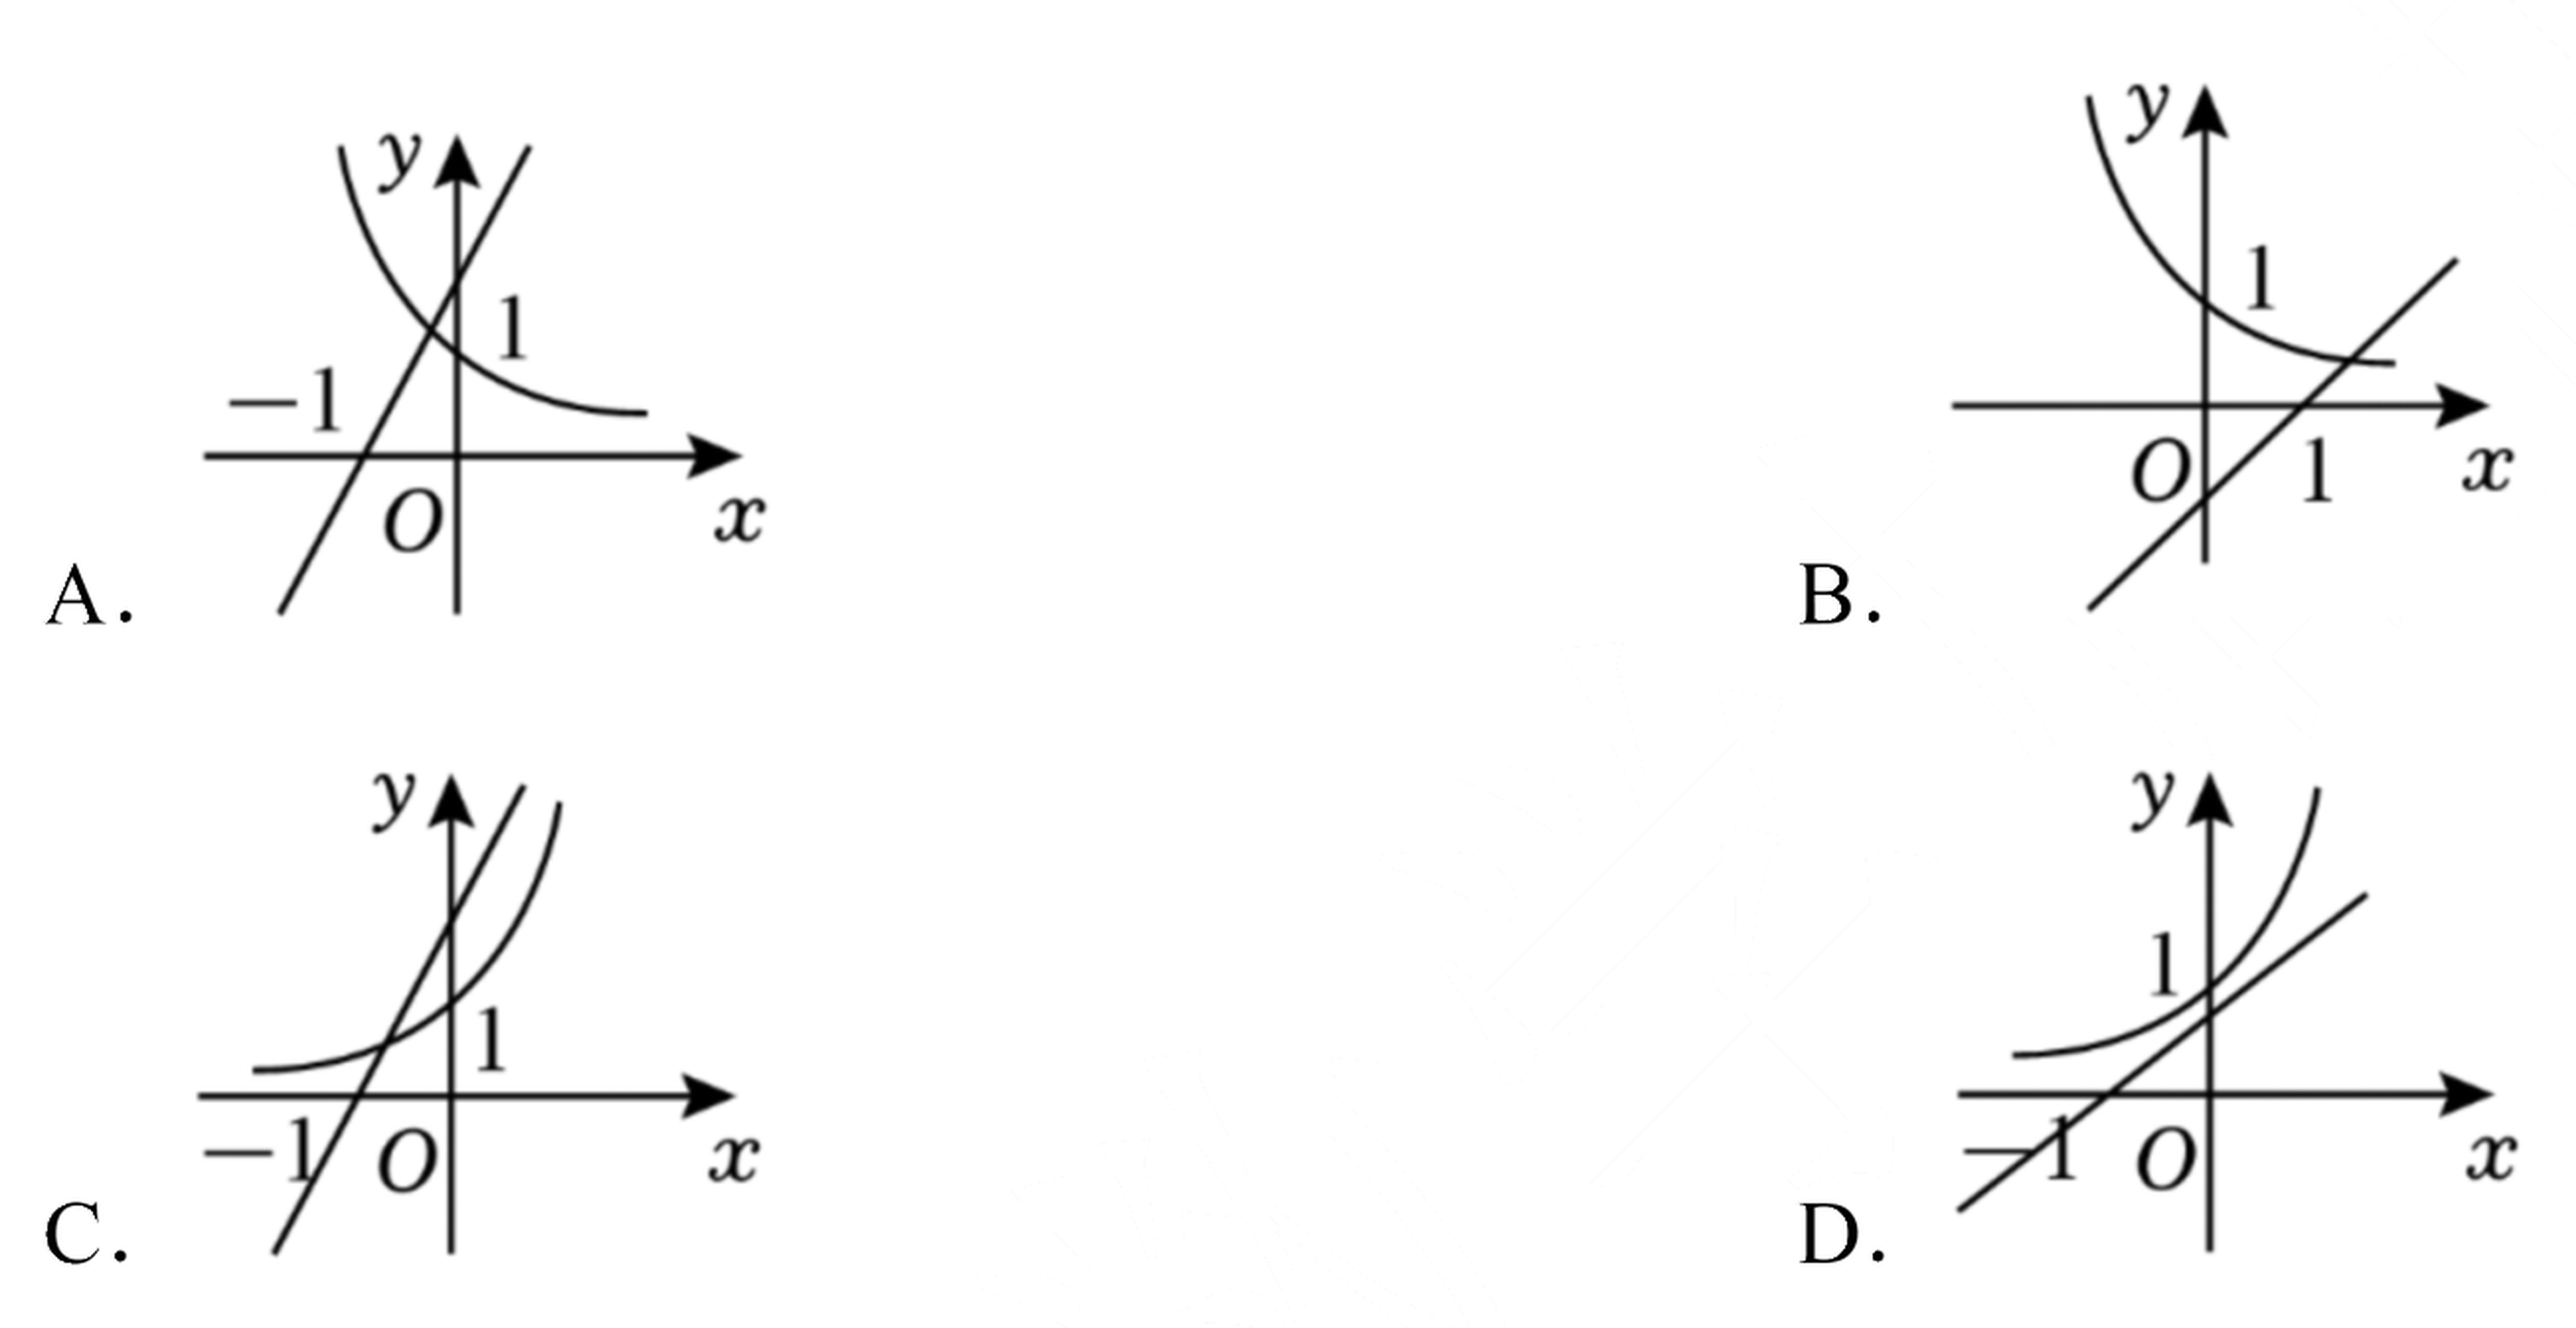
\includegraphics[width=0.80\textwidth]{figures/gao142_q15.png}
\end{center}

\ifanswer
\solbegin
\step{$A$ 中，由指数函数 $y=a^x(a>0\text{ 且 }a\neq1)$ 图像递减得 $0<a<1$，}
\step{而一次函数 $y=a(x+1)$ 的图像与 $y$ 轴交点纵坐标为 $a>1$，二者矛盾，}
\step{所以 $A$ 错；}
\step{由一次函数 $y=a(x+1)$ 的图像与 $x$ 轴交点横坐标为 $-1$，排除 $B$；}
\step{$C$ 中，由指数函数 $y=a^x(a>0\text{ 且 }a\neq1)$ 图像递减得 $a>1$，}% 原卷"递减得 a>1"自相矛盾（递减应得 0<a<1），照录
\step{而一次函数 $y=a(x+1)$ 的图像与 $y$ 轴交点纵坐标为 $a>1$，二者 $a$ 值吻合，}
\step{所以 $C$ 对；}
\step{$D$ 中，由一次函数 $y=a(x+1)$ 的图像得 $a=1$，与 $a>0$ 且 $a\neq1$ 矛盾，}
\step{所以 $D$ 错.}
\step{故选 $C$.}
\solend
\fi

\item 不等式 $\lvert x+1\rvert+\lvert 2-x\rvert\geqslant a^2-2a$ 恒成立，则 $a$ 的取值范围是\mbox{（\quad）}

\keepwithprev
A. $[-1,3]$\qquad B. $(-\infty,3]\cup[3,+\infty)$\qquad C. $(-\infty,3)$\qquad D. $(3,+\infty)$

\ifanswer
\solbegin
\step{因为 $\lvert x+1\rvert+\lvert 2-x\rvert\geqslant\lvert(x+1)+(2-x)\rvert=3$，}
\step{所以 $\lvert x+1\rvert+\lvert 2-x\rvert$ 的最小值为 3，}
\step{因为 $\lvert x+1\rvert+\lvert 2-x\rvert\geqslant a^2-2a$ 恒成立，所以只需 $a^2-2a\leqslant3$，所以 $-1\leqslant a\leqslant3$，}
\step{所以 $a$ 的取值范围为 $[-1,3]$. 故选 $A$.}
\solend
\fi

\end{enumerate}

\bigsec{三、解答题}

\begin{enumerate}
\setcounter{enumi}{16}

\item 已知集合 $A=\left\{x\mid\dfrac{x-3}{x-1}\leqslant0\right\}$，$B=\{x\mid\lvert x-1\rvert<a\}$.

(1) 若 $a=1$，求 $A\cap B$；

(2) 若 $x\in A$ 是 $x\in B$ 的充分条件，求 $a$ 的取值范围.

\ifanswer
\solbegin
\step{(1) 不等式 $\dfrac{x-3}{x-1}\leqslant0$，等价于 $(x-3)(x-1)\leqslant0$ 且 $x-1\neq0$，解得 $1<x\leqslant3$，}
\step{所以 $A=\{x\mid 1<x\leqslant3\}$，}
\step{当 $a=1$ 时，不等式 $\lvert x-1\rvert<a$ 可化为 $\lvert x-1\rvert<1$，所以 $-1<x-1<1$，}
\step{故 $0<x<2$，所以 $B=\{x\mid 0<x<2\}$，}
\step{所以 $A\cap B=\{x\mid 1<x<2\}$；}
\step{(2) 因为 $x\in A$ 是 $x\in B$ 的充分条件，所以 $A\subseteq B$，}% 子集符号原卷印带下划线 $\subseteq$，照录
\step{因为 $A=\{x\mid 1<x\leqslant3\}\neq\varnothing$，所以 $B\neq\varnothing$，故 $a>0$，}
\step{由不等式 $\lvert x-1\rvert<a$，解得 $1-a<x<1+a$，}
\step{所以 $B=\{x\mid 1-a<x<1+a\}$，所以 $\begin{cases}1-a\leqslant1\\1+a>3\end{cases}$，解得 $a>2$，}
\step{所以 $a$ 的取值范围为 $(2,+\infty)$.}
\solend
\fi

\item 计算下列式子的值（请务必书写必要的计算步骤）

(1) $27^{\frac13}+\left(\dfrac76\right)^0+\sqrt{(3-\pi)^2}$；

(2) $\lg25+\lg4+7^{\log_7 2}-\log_2 3\times\log_3 4+\log_3 9$.

\ifanswer
\solbegin
\step{(1) $27^{\frac13}+\left(\dfrac76\right)^0+\sqrt{(3-\pi)^2}=3^{3\times\frac13}+1+\lvert 3-\pi\rvert=3+1+\pi-3=\pi+1$；}
\step{(2) 原式 $=\lg(25\times4)+2-\dfrac{\lg3}{\lg2}\times\dfrac{\lg4}{\lg3}+2=\lg100+2-\dfrac{2\lg2}{\lg2}+2$}
\step{$=2+2-2+2=4$.}
\solend
\fi

\item 已知关于 $x$ 的不等式 $mx^2-(3m^2-m+2)x+6m-2\geqslant0$.

(1) 当 $m=2$ 时，求关于 $x$ 的不等式的解集；

(2) 当 $m>0$ 时，求关于 $x$ 的不等式的解集.

\ifanswer
\solbegin
\step{(1) $m=2$ 时，不等式为 $x^2-6x+5\geqslant0$，即 $(x-1)(x-5)\geqslant0$，}
\step{解得 $x\leqslant1$ 或 $x\geqslant5$，所以不等式的解集是 $\{x\mid x\leqslant1$ 或 $x\geqslant5\}$.}
\step{(2) $m>0$ 时，不等式可化为 $(mx-2)[x-(3m-1)]\geqslant0$，}
\step{即 $\left(x-\dfrac2m\right)[x-(3m-1)]\geqslant0$，}
\step{若 $m=1$，则不等式为 $(x-2)^2\geqslant0$，解得 $x\in\R$；}
\step{若 $0<m<1$，则 $\dfrac2m>3m-1$，解不等式得 $x\geqslant\dfrac2m$ 或 $x\leqslant3m-1$；}
\step{若 $m>1$，则 $\dfrac2m<3m-1$，解不等式得 $x\geqslant3m-1$ 或 $x\leqslant\dfrac2m$；}
\step{综上，$0<m<1$ 时，不等式的解集是 $\{x\mid x\leqslant3m-1$ 或 $x\geqslant\dfrac2m\}$；}
\step{$m=1$ 时，不等式的解集为 $\R$；}
\step{$m>1$ 时，不等式的解集是 $\{x\mid x\leqslant\dfrac2m$ 或 $x\geqslant3m-1\}$.}
\solend
\fi

\item 如图，某人计划用篱笆围成一个一边靠墙（墙足够长）的矩形菜园. 设菜园的长为 $x$ 米，宽为 $y$ 米.

\begin{center}
% 矩形围栏示意图取原卷 07 页截图去粉色水印、去色、LANCZOS 放大；题目配图，三版都出
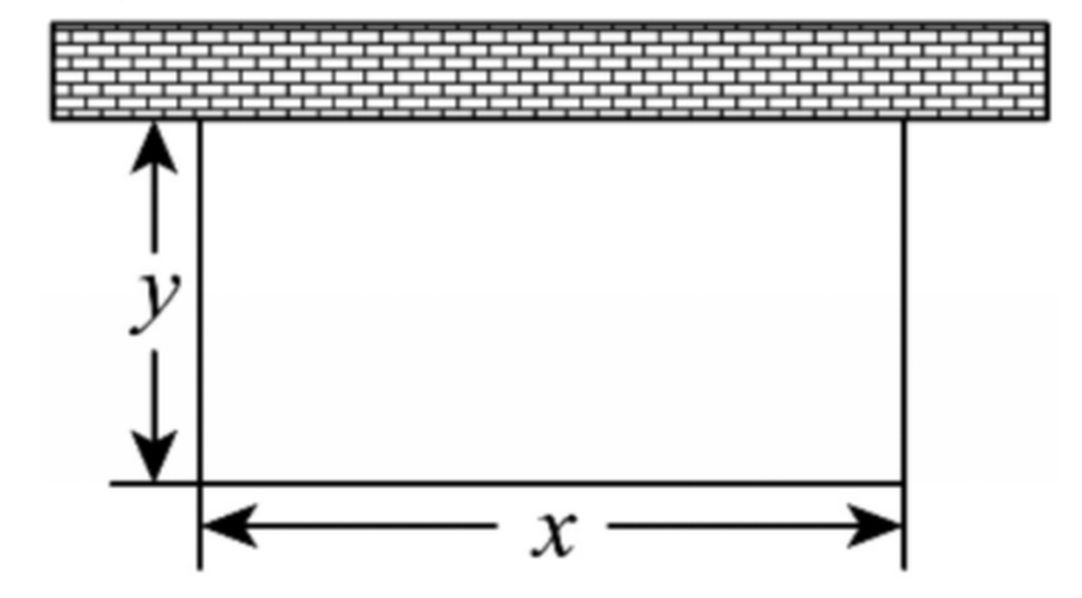
\includegraphics[width=0.42\textwidth]{figures/gao142_q20.png}
\end{center}

(1) 若菜园面积为 72 平方米，则 $x$、$y$ 为何值时，所用篱笆总长最小？

(2) 若 $x$、$y$ 满足 $x+y-xy+63=0$，则菜园面积最小为多少平方米？

\ifanswer
\solbegin
\step{(1) 由题意得，菜园的面积 $S=xy=72$，且 $x>0$，$y>0$，}
\step{所用篱笆总长 $L=x+2y$，}
\step{由基本不等式得 $x+2y\geqslant2\sqrt{x\cdot2y}=2\sqrt{2xy}=2\sqrt{2\times72}=24$，}
\step{当且仅当 $x=2y$ 时取等号，}
\step{联立 $\begin{cases}xy=72\\x=2y\end{cases}$，解得 $\begin{cases}x=12\\y=6\end{cases}$，}
\step{所以当 $x=12$，$y=6$ 时，所用篱笆总长最小；}
\step{(2) 由题意得 $x>0$，$y>0$，且满足 $x+y-xy+63=0$，即 $x+y=xy-63$，}
\step{由基本不等式得 $x+y\geqslant2\sqrt{xy}$，当且仅当 $x=y$ 时取等号，}
\step{所以 $xy-63\geqslant2\sqrt{xy}$. 令 $t=\sqrt{xy}(t>0)$，则 $xy=t^2$，}
\step{上述不等式可化为 $t^2-2t-63\geqslant0$，即 $(t-9)(t+7)\geqslant0$，}
\step{因为 $t>0$，所以 $t+7>0$，故 $t-9\geqslant0$，解得 $t\geqslant9$，所以 $\sqrt{xy}\geqslant9$，}
\step{即 $xy\geqslant81$，当且仅当 $x=y=9$ 时取等号，此时满足 $9+9-81+63=0$，}
\step{所以菜园面积最小为 81 平方米.}
\solend
\fi

\item 已知幂函数 $f(x)=(m^2-3m+3)x^m$ 的图象关于 $y$ 轴对称.

(1) 求实数 $m$ 的值；

(2) 在平面直角坐标系中作出函数 $y=\lvert f(x)-1\rvert$ 的图象；

(3) 已知点 $A(2a,y_1)$ 与点 $B(3-a,y_2)$ 都在幂函数 $y=x^2$ 的图象上. 若 $y_1<y_2$，求实数 $a$ 的取值范围.

\begin{center}
% 空白坐标网格取原卷 08 页截图去粉色水印、去色、LANCZOS 放大；题目配图，三版都出
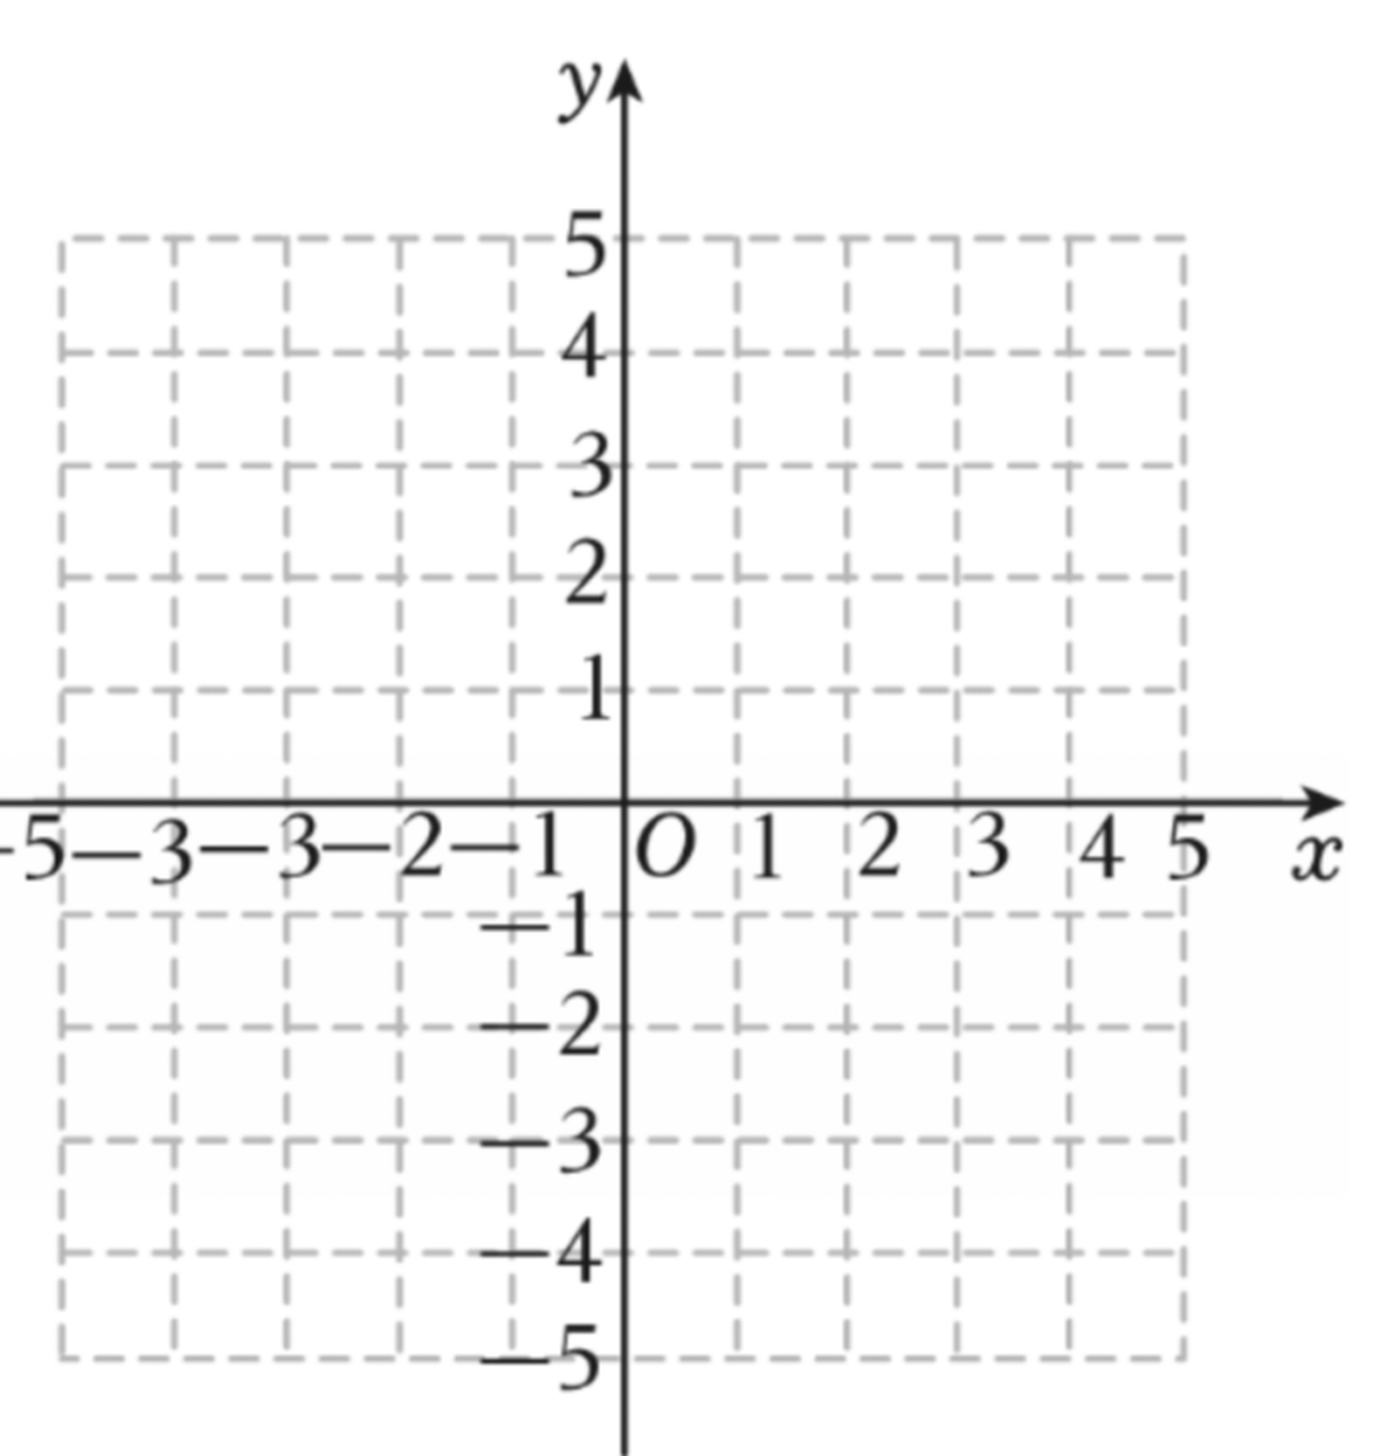
\includegraphics[width=0.52\textwidth]{figures/gao142_q21_grid.png}
\end{center}

\ifanswer
\solbegin
\step{(1) 由题意幂函数 $f(x)=(m^2-3m+3)x^m$，}
\step{故 $m^2-3m+3=1$，解得 $m=1$ 或 $m=2$，}
\step{又 $f(x)$ 图象关于 $y$ 轴对称，即 $f(x)$ 是偶函数，}
\step{当 $m=1$ 时，$f(x)=x$ 是奇函数，不满足条件，舍去；}
\step{当 $m=2$ 时，$f(x)=x^2$ 是偶函数，满足条件，故 $m=2$；}
\step{(2) 由 (1) 得，$\lvert f(x)-1\rvert=\lvert x^2-1\rvert$，}
\step{先画 $y=x^2-1$，开口向上的抛物线，顶点 $(0,-1)$，零点 $x=\pm1$，}
\step{再将 $x$ 轴下方的部分沿 $x$ 轴翻折到上方即为 $y=\lvert x^2-1\rvert$ 的图象，}
\step{图象如图所示.}
\par{\leftskip=0pt
\begin{center}
% 抛物线图象取原卷 09 页截图去粉色水印、去色、LANCZOS 放大；解析所附配图，仅答案版出
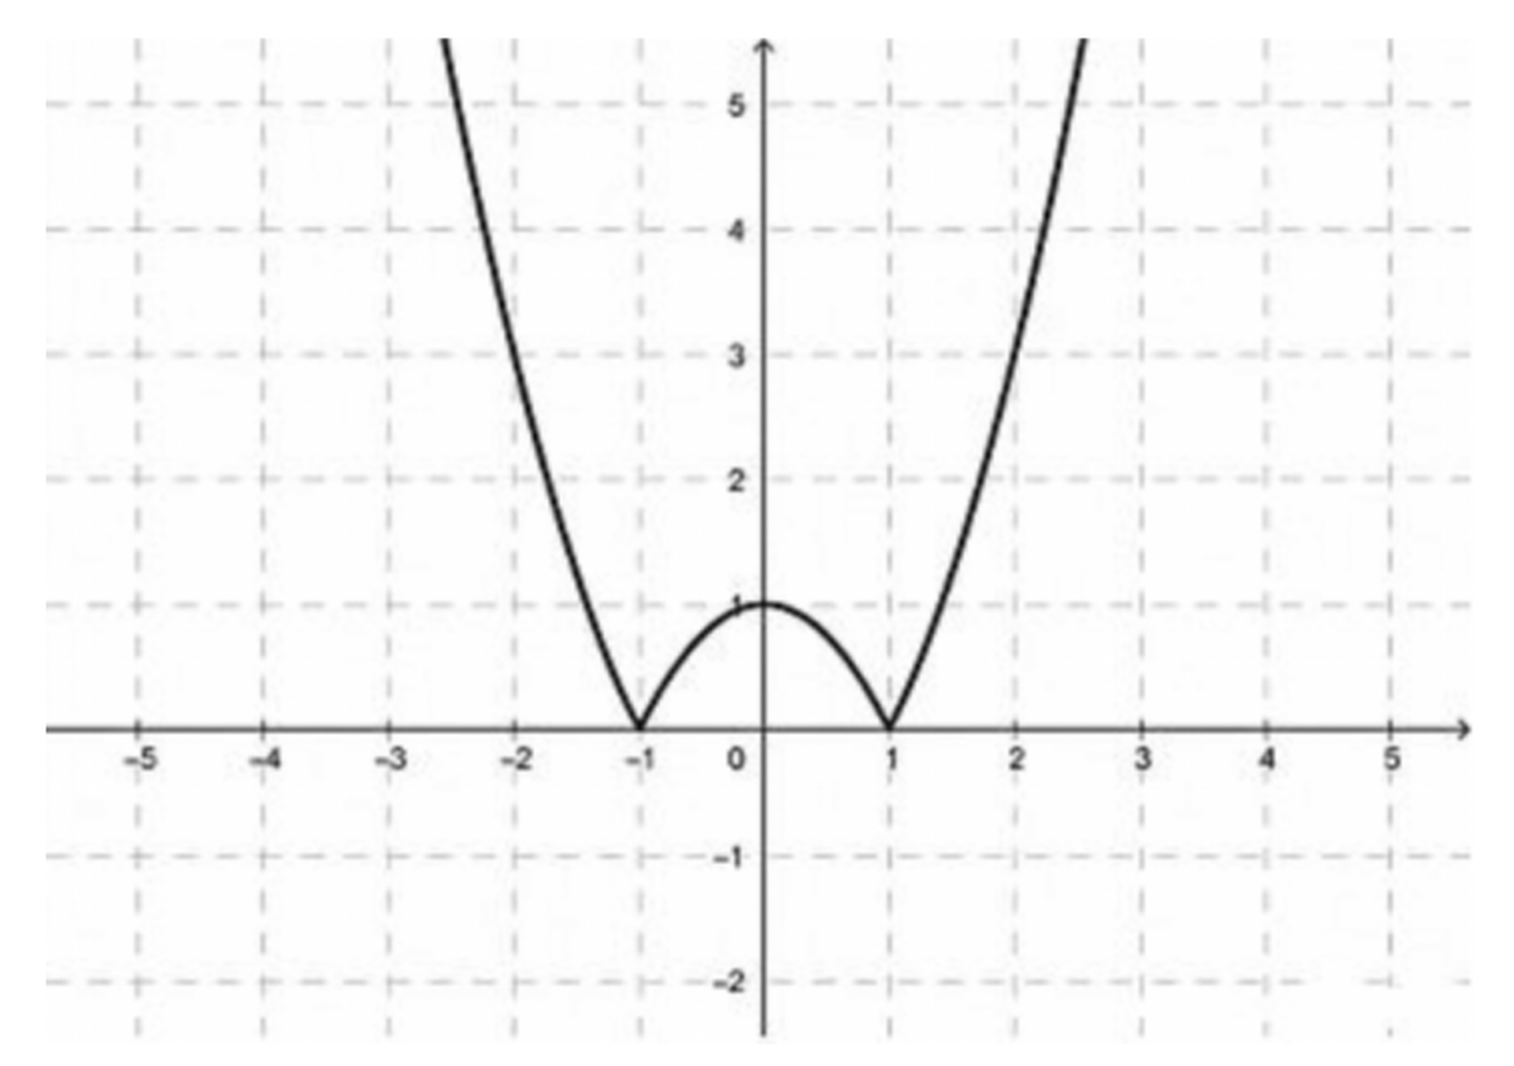
\includegraphics[width=0.55\textwidth]{figures/gao142_q21_para.png}
\end{center}}
\step{(3) 由题意得，$y_1=(2a)^2$，$y_2=(3-a)^2$，}
\step{$y_1<y_2$，即有 $(2a)^2<(3-a)^2$，化简整理得 $(a+3)(a-1)<0$，}
\step{解得实数 $a$ 的取值范围为 $(-3,1)$.}
\solend
\fi

\end{enumerate}

\end{document}
"
% 紧凑版：xelatex "\def\iscompact{1}% 高一142_群峰高级中学_期中.tex
%   —— 高一上数学"2026-2027 年群峰高级中学高一上期中"（试卷版/答案版）
% 试卷版：xelatex 高一142_群峰高级中学_期中.tex
% 答案版：xelatex "\def\isanswer{1}% 高一142_群峰高级中学_期中.tex
%   —— 高一上数学"2026-2027 年群峰高级中学高一上期中"（试卷版/答案版）
% 试卷版：xelatex 高一142_群峰高级中学_期中.tex
% 答案版：xelatex "\def\isanswer{1}% 高一142_群峰高级中学_期中.tex
%   —— 高一上数学"2026-2027 年群峰高级中学高一上期中"（试卷版/答案版）
% 试卷版：xelatex 高一142_群峰高级中学_期中.tex
% 答案版：xelatex "\def\isanswer{1}\input{高一142_群峰高级中学_期中.tex}"
% 紧凑版：xelatex "\def\iscompact{1}\input{高一142_群峰高级中学_期中.tex}"
%
% ① 原始材料：微信公众号"魔都数学加油站"文章，连载"27学年高一142"，原文标题
% "27学年高一142——2026-2027年上海市群峰高级中学高一上期中"；
% 原文链接：https://mp.weixin.qq.com/s/cc7wnuP4Pk3OjNDV6ihB9A。
% 正文为 9 张 PNG 页（01、02、04、06、07、08、09 为 2560x3620；03、05 为 4762x6735，
% 同一篇各页分辨率不同，逐页按各自分辨率裁图核对），题目下印有【答案】或【解析】，为讲评版。
% 题目、解析均据原图转录；卷面粉红色水印"魔都数学加油站"及公众号页脚未录入。
% 全卷 4 幅插图：第 15 题四幅坐标函数图像选项（04 页，2x2 合并为一张）、
% 第 20 题矩形围栏示意图（07 页）、第 21 题 (2) 空白坐标网格（08 页）、
% 第 21 题抛物线图象（09 页，解析所附图）；均取原卷截图去粉色水印、LANCZOS 放大。
% 题目配图三版都出、解析配图仅答案版出。
%
% 卷首标题：原卷印作"2026-2027 年群峰高级中学高一上期中"（公众号标题中的"上海市"
% 卷面标题行没有，本稿照卷面），年份区间按全稿惯例排 en dash；原卷未印副标题，
% 本卷为期中卷、跨集合与常用逻辑用语／不等式／函数三章，按题目内容补出
% "集合与常用逻辑用语、不等式、函数"（头注说明，与同期中卷口径相同）。
%
% 题号体例：本卷共 19 题——一、填空题 3—12（10 题）、二、选择题 13—16（4 题）、
% 三、解答题 17—21（5 题）。三节分别 \setcounter{enumi}{2}／{12}／{16}。
% 原卷从第 3 题起、无第 1、2 题，本稿保留原题号。
%
% ② 与原卷的排版差异：
%   ① 原文从第 3 题起，本稿保留原题号；原卷未印副标题，本稿按"知识模块"口径补出；
%   ② 逐题答案口径：Q14 原卷把答案 D 印在题干括号内、且题目下无【解析】，本稿括号
%      留空 \mbox{（\quad）}、另提 \ans{D}；Q13／Q15／Q16 答案在【解析】末句"故选 …"
%      （分别为 C／C／A），题干括号留空、不另提 \ans{}；其余各题（Q3—Q12、
%      Q17—Q21）题目下印【解析】、答案融在解析中，不另提 \ans{}；全卷仅 Q14 一处 \ans{}；
%      答案版【答案】/【解析】标记数 = 19（1 个 \ans + 18 个 \solbegin）= 全卷题数；
%   ③ 原卷填空横线按全稿惯例排 \blankline[4.4em]；选择题括号排 \mbox{（\quad）}、
%      每个选项段前按惯例加 \keepwithprev（Q15 四幅图那一枚放在 \begin{center} 之前）；
%      解答题不留作答区、不加 \anspace（原卷为讲评版，与 129／131／132／133／136／140 同）；
%   ④ 原卷数集斜体 $R$（Q5、Q7、Q19、Q21 解析等）按全稿惯例统一改 \R；空集记号
%      \varnothing；绝对值排 \lvert…\rvert，集合描述竖线排 \mid；不等号按全稿惯例
%      排 \leqslant／\geqslant；
%   ⑤ 4 幅插图：Q15 四幅坐标函数图象选项合并裁为一张 \includegraphics（题前
%      \needvspace{9cm}）；Q15 是"二、选择题"节内带大图块的第 3 题（Q13、Q14 在前
%      且无图），另在 \bigsec{二、选择题} 之前加 \needvspace{11cm} 连节标题一起量
%      ——守卫必须放在 \bigsec 之前，放标题之后会让"二、选择题"孤立在页末
%      （B 类，照 高一26／40／59／136／140 成例）；Q20 围栏图与 Q21 网格图置于题干
%      之后（三版都出），Q21 抛物线图置于答案版解析 (2) 与 (3) 之间（仅答案版出）；
%   ⑥ 子题标号按原卷排半角 (1)(2)(3)（与 140／141 同期中卷口径相同）；括注全角／
%      半角逐处照录：Q3"（用含有 m 的代数式表示）"、Q6"（舍）"、Q10"（万元）"、
%      Q18"（请务必书写必要的计算步骤）"、Q20"（墙足够长）"印全角；Q15
%      "$y=a^x(a>0 且 a\neq1)$"、Q10"$y=x^a(a 为常数)$"、Q20"$t=\sqrt{xy}(t>0)$"
%      等数学式内括注印半角；数学式内 CJK 用 \text{…}（否则 FONTCHK 报缺字）；
%   ⑦ 数学式内半角逗号照录（如 Q6"$ax-1=0,a\in\R$"、Q9"$b=2+\sqrt2,a=\sqrt2+1$"、
%      Q16 区间 "$[-1,3]$"、Q21"$y_1<y_2$，即 $(2a)^2<(3-a)^2$" 等）；原卷行末
%      西文句点照录（Q7"(-3,5)."、Q10"125（万元）."、Q19 题干句点、Q20 题干
%      "矩形菜园."与"宽为 y 米."、Q21 题干"对称." 等）；行中全角逗号、分号照录；
%   ⑧ 题干中的中文弯引号：本卷题干与解析通篇未出现中文弯引号，故无此项；
%      圈数字 ①②③ 亦未出现（子题用 (1)(2)(3)）；
%   ⑨ 原卷"图像／图象"两种写法混用，逐处放大核对并照录：Q4 题干与解析作"图象"、
%      Q7 解析作"图象"、Q8 题干作"图像"而解析作"图象"、Q15 题干与解析通篇作
%      "图像"、Q21 题干与解析通篇作"图象"；
%   ⑩ 原卷无红色加粗标签（【解析】均黑色印刷；逐页扫描深红像素为 0），故本卷未用
%      \stepm；黑色常规分步标签（"A 中""C 中""D 中""(1)(2)(3)" 等）按普通 \step
%      行内文字照录；
%   ⑪ 跨页续印按题合并，明细见 ⑥。
%
% ③ 行数复核：一条 \step = 原卷解析的一个印刷行，cases 块作一个印刷行计。逐题数 \step
%   条数，合计 98 条（Q3：1；Q4：2；Q5：3；Q6：4；Q7：5；Q8：2；Q9：4；Q10：3；
%   Q11：4；Q12：3；Q13：5；Q14：0；Q15：10；Q16：4；Q17：10；Q18：3；
%   Q19：10；Q20：13；Q21：12），与原卷印刷行逐题相等。Q14 只把答案印在题干括号、
%   无【解析】，提 \ans{D}、不计入 \step 账；答案版标记数 = 19（1 个 \ans + 18 个
%   \solbegin）= 全卷题数。
%
% ④ 判别式字形：全卷判别式共 3 处——第 7 题【解析】"即判别式△<0"、
%   "即△=(a-1)^2-4×1×4<0" 两处原卷印扁等边三角 $\triangle$，
%   第 11 题【解析】cases 块"△=4a^2-4(a+6)≥0" 一处原卷印等腰偏高的高三角 $\Delta$；
%   逐处放大核对，两形不同、全卷混用，本稿逐处照录不统一（参照 高一141 头注④口径）。
%   子集符号：全卷共 3 处——第 6 题题干"若 B⊆A"、第 6 题【解析】"因为 B⊆A"、
%   第 17 题【解析】(2)"所以 A⊆B"，逐处放大核对，原卷三处均印带下划线的
%   $\subseteq$（不是单线 $\subset$），本稿一律照录 \subseteq；全卷未出现 \subset。
%
% ⑤ 原卷存疑照录（均照录未改，正文对应处另有 % 注）：
%   第 14 题题干括号内原卷印答案 D（非留空），且题目下无【解析】，按"答案印括号且
%      无解析"口径括号留空、另提 \ans{D}；
%   第 15 题【解析】"C 中，由指数函数 … 图像递减得 a>1" 中"递减"与"a>1"
%      自相矛盾（递减应得 0<a<1，疑为"递增"之误），照录；
%   第 16 题选项 B 作 $(-\infty,3]\cup[3,+\infty)$，两端区间并起即全体实数、
%      与正确答案 $[-1,3]$ 不成干扰项（疑为 $(-\infty,-1]\cup[3,+\infty)$ 之误），照录；
%   第 21 题 (2) 空白坐标网格的 x 轴刻度原卷印作"-5 -3 -3 -2 -1 0 1 2 3 4 5"
%      （"-3"重复，疑为"-4"之误），系插图中的印刷内容，取原卷截图照录、不改图。
%
% ⑥ 跨页续印说明：Q7 题干与解析首行在 01 页、解析续至 02 页；Q11 题干与解析
%   4 行在 03 页；Q13 解析前 4 行在 03 页、末句"故选 C."续至 04 页；Q15 题干与
%   四幅图在 04 页、解析前 8 行在 04 页、末 2 行续至 05 页；Q17 解析前 7 行在
%   05 页、后 3 行续至 06 页；Q19 解析前 5 行在 06 页、后 5 行续至 07 页；
%   Q20 解析前 9 行在 07 页、后 4 行续至 08 页；Q21 解析 (1)(2) 9 行在 08 页、
%   抛物线图与 (3) 3 行续至 09 页；本稿按题连排，不丢行。三版切页审计结论见
%   编译自验回报（切页守卫见 ②⑤）。
%
\documentclass[a4paper,11pt]{article}
\usepackage{common}

\begin{document}

\examtitlest[3]{2026--2027 年群峰高级中学高一上期中}{集合与常用逻辑用语、不等式、函数}

\bigsec{一、填空题}

\begin{enumerate}
\setcounter{enumi}{2}

\item 已知 $\log_2 3=m$，则 $\log_3 6=$\blankline[4.4em]（用含有 $m$ 的代数式表示）.

\ifanswer
\solbegin
\step{$\log_3 6=\dfrac{\log_2 6}{\log_2 3}=\dfrac{\log_2 2+\log_2 3}{\log_2 3}=\dfrac{1+m}{m}=\dfrac1m+1$.}
\solend
\fi

\item 若指数函数 $y=a^x$ 的图象经过点 $(3,27)$，则 $a$ 的值为\blankline[4.4em].

\ifanswer
\solbegin
\step{因为指数函数 $y=a^x$ 的图象经过点 $(3,27)$，}
\step{所以 $a^3=27=3^3$，所以 $a=3$.}
\solend
\fi

\item 不等式 $(2x+1)^{\frac13}<(3-x)^{\frac13}$ 的解集为\blankline[4.4em].

\ifanswer
\solbegin
\step{因为幂函数 $f(t)=t^{\frac13}$ 在 $\R$ 上严格增，}
\step{所以原不等式等价于 $2x+1<3-x$，解得 $x<\dfrac23$，}
\step{因此原不等式的解集为 $\left(-\infty,\dfrac23\right)$.}
\solend
\fi

\item 设集合 $A=\{1,-2\}$，$B=\{x\mid ax-1=0,a\in\R\}$，若 $B\subseteq A$，则 $a$ 的值为\blankline[4.4em].% 子集符号原卷印带下划线 $\subseteq$，照录

\ifanswer
\solbegin
\step{因为 $B\subseteq A$，所以 $B=\varnothing$ 或 $\{-2\}$ 或 $\{1\}$ 或 $\{1,-2\}$（舍），}% 子集符号原卷印带下划线 $\subseteq$，照录
\step{若 $B=\varnothing$，则 $a=0$；若 $B=\{1\}$，则 $a=1$；}
\step{若 $B=\{-2\}$，则 $-2a=1$，解得 $a=-\dfrac12$；}
\step{综上，$a=0$ 或 $1$ 或 $-\dfrac12$.}
\solend
\fi

\item 不等式 $x^2+(a-1)x+4>0$ 在 $\R$ 上恒成立，则实数 $a$ 的取值范围是\blankline[4.4em].

\ifanswer
\solbegin
\step{不等式 $x^2+(a-1)x+4>0$，对应的二次函数为 $y=x^2+(a-1)x+4$，}
\step{因此函数图象开口向上，要使不等式对任意实数 $x$ 恒成立，}
\step{需二次函数图象与 $x$ 轴无交点，即判别式 $\triangle<0$，}% 判别式原卷印扁等边三角 $\triangle$，照录
\step{即 $\triangle=(a-1)^2-4\times1\times4<0$，整理得 $a^2-2a-15<0$，}% 判别式原卷印扁等边三角 $\triangle$，照录
\step{解得 $-3<a<5$，故实数 $a$ 的取值范围是 $(-3,5)$.}
\solend
\fi

\item 函数 $f(x)=(5x-3)^a$ 的图像恒过点\blankline[4.4em].% 题干作"图像"、解析作"图象"，原卷混用，逐处照录

\ifanswer
\solbegin
\step{令 $5x-3=1$ 得 $x=\dfrac45$，此时 $f\left(\dfrac45\right)=\left(5\times\dfrac45-3\right)^a=1$，}
\step{所以 $f(x)$ 的图象恒过 $\left(\dfrac45,1\right)$.}
\solend
\fi

\item 若 $a>0$，$b>0$ 且 $\dfrac1a+\dfrac2b=1$，则 $a+b$ 的最小值为\blankline[4.4em].

\ifanswer
\solbegin
\step{因为 $a>0$，$b>0$，$\dfrac1a+\dfrac2b=1$，}
\step{所以 $a+b=(a+b)\left(\dfrac1a+\dfrac2b\right)=1+\dfrac{2a}{b}+\dfrac{b}{a}+2\geqslant3+2\sqrt{\dfrac{2a}{b}\cdot\dfrac{b}{a}}=3+2\sqrt2$，}
\step{当且仅当 $\dfrac{2a}{b}=\dfrac{b}{a}$，即 $b=2+\sqrt2,a=\sqrt2+1$ 时取等号，}
\step{故 $a+b$ 的最小值为 $3+2\sqrt2$.}
\solend
\fi

\item 某药厂研制出一种新型药剂，投放市场后其广告投入 $x$（万元）与药品利润 $y$（万元）存在的关系为 $y=x^a(a\text{ 为常数})$，其中 $x$ 不超过 5 万元. 已知去年投入广告费用为 3 万元时，药品利润为 27 万元，若今年投入广告费用 5 万元，预计今年药品利润为\blankline[4.4em]万元.

\ifanswer
\solbegin
\step{由已知投入广告费用为 3 万元时，药品利润为 27 万元，}
\step{代入 $y=x^a$ 中，即 $3^a=27$，解得 $a=3$，故函数关系式为 $y=x^3$，}
\step{所以当 $x=5$ 时，$y=125$（万元）.}
\solend
\fi

\item 已知方程 $x^2+2ax+a+6=0$ 的两根分别是 $x_1$ 和 $x_2$，且满足 $\dfrac1{x_1}+\dfrac1{x_2}<0$，则实数 $a$ 的取值范围是\blankline[4.4em].

\ifanswer
\solbegin
\step{由于方程 $x^2+2ax+a+6=0$ 的两根分别是 $x_1$ 和 $x_2$，}
\step{则 $\begin{cases}\Delta=4a^2-4(a+6)\geqslant0\\x_1+x_2=-2a\\x_1x_2=a+6\end{cases}$，解得 $a\geqslant3$ 或 $a\leqslant-2$.}% 判别式原卷印等腰偏高的高三角 $\Delta$，照录（与第 7 题扁等边 $\triangle$ 两形混用）
\step{又 $\dfrac1{x_1}+\dfrac1{x_2}<0$，即 $\dfrac{x_1+x_2}{x_1\cdot x_2}<0$，故 $\dfrac{-2a}{a+6}<0$，解得 $a<-6$ 或 $a>0$.}
\step{综上，$a$ 的取值范围是 $(-\infty,-6)\cup[3,+\infty)$.}
\solend
\fi

\item 已知 $b>a>1$，若 $\log_a b-\log_b a=\dfrac32$，$a^b=b^a$，则 $a-b=$\blankline[4.4em].

\ifanswer
\solbegin
\step{因为 $b>a>1$，所以 $\log_a b>1$，}
\step{由 $\log_a b-\log_b a=\log_a b-\dfrac{1}{\log_a b}=\dfrac32$，解得 $\log_a b=2$ 即 $b=a^2$，}
\step{因为 $a^b=b^a=a^{2a}$，所以 $b=2a=a^2$，所以 $a=2$，$b=4$，则 $a-b=-2$.}
\solend
\fi

\end{enumerate}

% 第 15 题四幅图是"二、选择题"节内的大图块；守卫须放在 \bigsec 之前连节标题一起量
\needvspace{11cm}
\bigsec{二、选择题}

\begin{enumerate}
\setcounter{enumi}{12}

\item 若 $a>b$，$c<0$，则下列不等式正确的是\mbox{（\quad）}

\keepwithprev
A. $ab>bc$\qquad B. $a+c<b+c$\qquad C. $ac^2>bc^2$\qquad D. $\dfrac ac>\dfrac bc$

\ifanswer
\solbegin
\step{因为 $a>b$，$c<0$，取 $b=0$，则 $ab=bc=0$，故 $A$ 错误；}
\step{由于 $a>b$，所以 $a+c>b+c$，故 $B$ 错误；}
\step{由 $c<0$ 得 $c^2>0$，所以 $ac^2>bc^2$，故 $C$ 正确；}
\step{由于 $a>b$ 且 $c<0$，所以 $\dfrac ac<\dfrac bc$，故 $D$ 错误.}
\step{故选 $C$.}
\solend
\fi

\item 若 $x>0$，$y>0$，则下列各式中，恒成立的是\mbox{（\quad）}% 原卷题干括号内印答案 D、且题目下无【解析】，本稿括号留空、另提 \ans{D}

\keepwithprev
A. $\lg x+\lg y=\lg(x+y)$\qquad B. $\lg x^2=(\lg x)^2$

C. $\dfrac{\lg x}{\lg y}=\lg(x-y)$\qquad D. $\lg x^{\frac1n}=\dfrac{\lg x}{n}$

\ifanswer
\ans{$D$}
\fi

% 第 15 题四幅坐标函数图象选项是一整块，守卫放在 \item 之前
\needvspace{9cm}
\item 在同一平面直角坐标系中，指数函数 $y=a^x(a>0\text{ 且 }a\neq1)$ 和一次函数 $y=a(x+1)$ 的图像关系可能是\mbox{（\quad）}

\keepwithprev
\begin{center}
% 四幅坐标函数图象选项取原卷 04 页截图去粉色水印、去色，按原卷 2x2 排布合并为一张
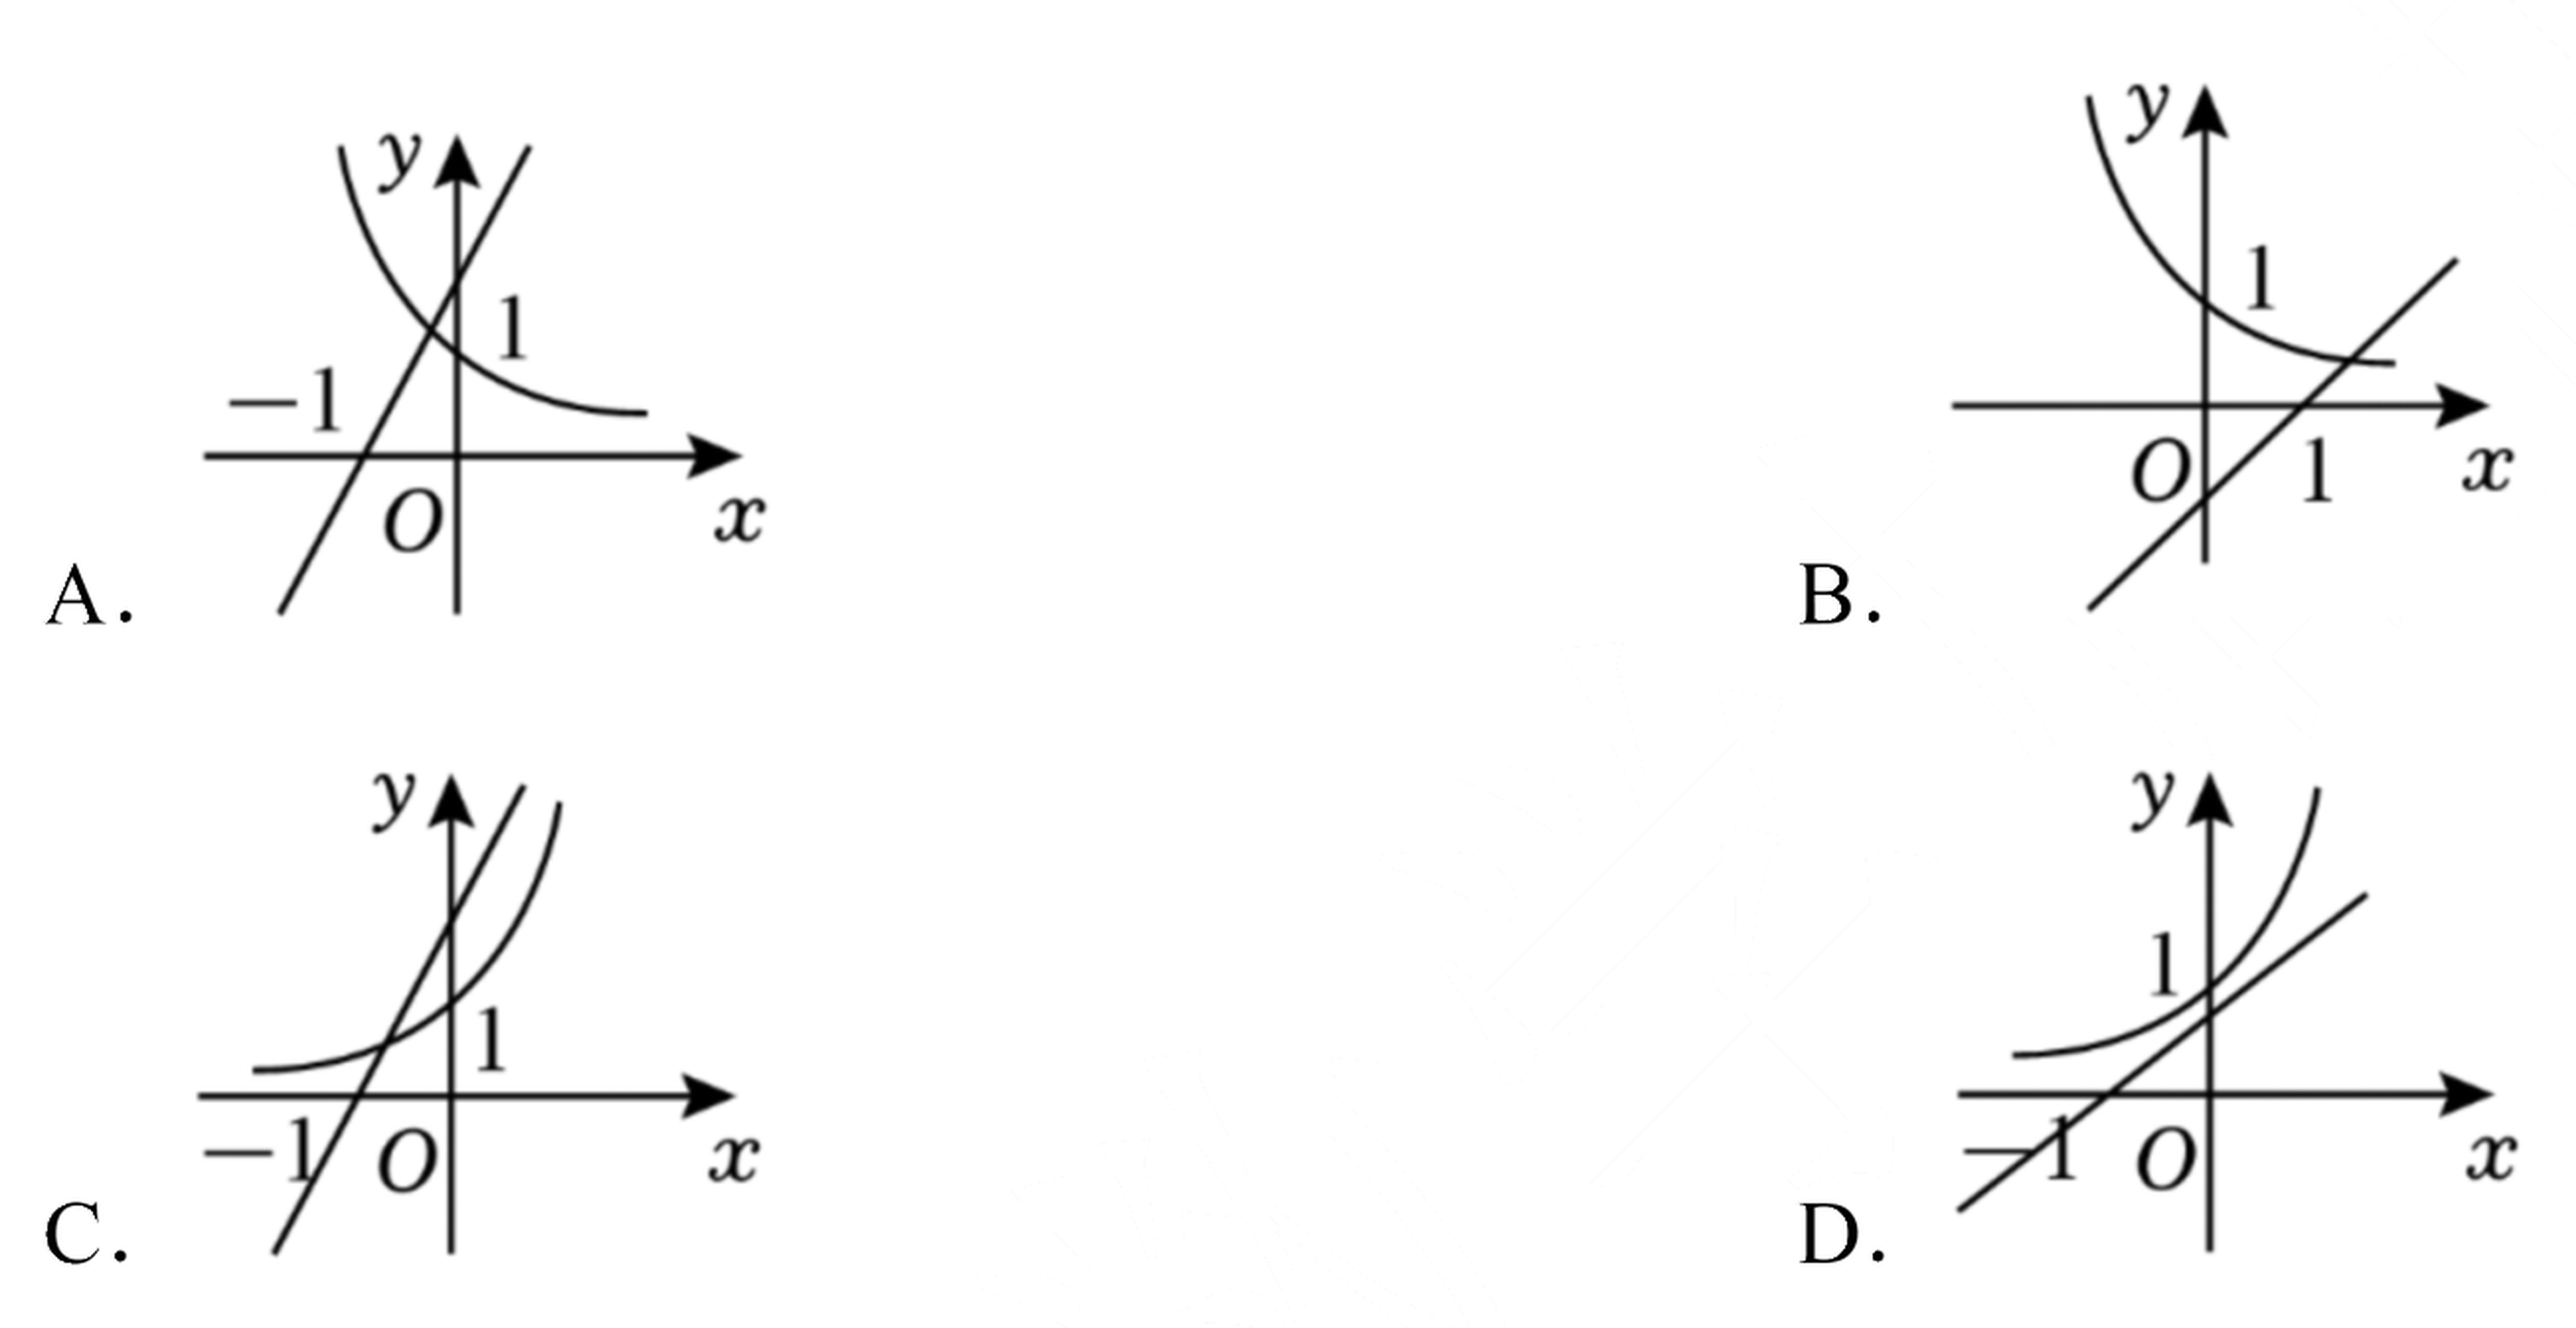
\includegraphics[width=0.80\textwidth]{figures/gao142_q15.png}
\end{center}

\ifanswer
\solbegin
\step{$A$ 中，由指数函数 $y=a^x(a>0\text{ 且 }a\neq1)$ 图像递减得 $0<a<1$，}
\step{而一次函数 $y=a(x+1)$ 的图像与 $y$ 轴交点纵坐标为 $a>1$，二者矛盾，}
\step{所以 $A$ 错；}
\step{由一次函数 $y=a(x+1)$ 的图像与 $x$ 轴交点横坐标为 $-1$，排除 $B$；}
\step{$C$ 中，由指数函数 $y=a^x(a>0\text{ 且 }a\neq1)$ 图像递减得 $a>1$，}% 原卷"递减得 a>1"自相矛盾（递减应得 0<a<1），照录
\step{而一次函数 $y=a(x+1)$ 的图像与 $y$ 轴交点纵坐标为 $a>1$，二者 $a$ 值吻合，}
\step{所以 $C$ 对；}
\step{$D$ 中，由一次函数 $y=a(x+1)$ 的图像得 $a=1$，与 $a>0$ 且 $a\neq1$ 矛盾，}
\step{所以 $D$ 错.}
\step{故选 $C$.}
\solend
\fi

\item 不等式 $\lvert x+1\rvert+\lvert 2-x\rvert\geqslant a^2-2a$ 恒成立，则 $a$ 的取值范围是\mbox{（\quad）}

\keepwithprev
A. $[-1,3]$\qquad B. $(-\infty,3]\cup[3,+\infty)$\qquad C. $(-\infty,3)$\qquad D. $(3,+\infty)$

\ifanswer
\solbegin
\step{因为 $\lvert x+1\rvert+\lvert 2-x\rvert\geqslant\lvert(x+1)+(2-x)\rvert=3$，}
\step{所以 $\lvert x+1\rvert+\lvert 2-x\rvert$ 的最小值为 3，}
\step{因为 $\lvert x+1\rvert+\lvert 2-x\rvert\geqslant a^2-2a$ 恒成立，所以只需 $a^2-2a\leqslant3$，所以 $-1\leqslant a\leqslant3$，}
\step{所以 $a$ 的取值范围为 $[-1,3]$. 故选 $A$.}
\solend
\fi

\end{enumerate}

\bigsec{三、解答题}

\begin{enumerate}
\setcounter{enumi}{16}

\item 已知集合 $A=\left\{x\mid\dfrac{x-3}{x-1}\leqslant0\right\}$，$B=\{x\mid\lvert x-1\rvert<a\}$.

(1) 若 $a=1$，求 $A\cap B$；

(2) 若 $x\in A$ 是 $x\in B$ 的充分条件，求 $a$ 的取值范围.

\ifanswer
\solbegin
\step{(1) 不等式 $\dfrac{x-3}{x-1}\leqslant0$，等价于 $(x-3)(x-1)\leqslant0$ 且 $x-1\neq0$，解得 $1<x\leqslant3$，}
\step{所以 $A=\{x\mid 1<x\leqslant3\}$，}
\step{当 $a=1$ 时，不等式 $\lvert x-1\rvert<a$ 可化为 $\lvert x-1\rvert<1$，所以 $-1<x-1<1$，}
\step{故 $0<x<2$，所以 $B=\{x\mid 0<x<2\}$，}
\step{所以 $A\cap B=\{x\mid 1<x<2\}$；}
\step{(2) 因为 $x\in A$ 是 $x\in B$ 的充分条件，所以 $A\subseteq B$，}% 子集符号原卷印带下划线 $\subseteq$，照录
\step{因为 $A=\{x\mid 1<x\leqslant3\}\neq\varnothing$，所以 $B\neq\varnothing$，故 $a>0$，}
\step{由不等式 $\lvert x-1\rvert<a$，解得 $1-a<x<1+a$，}
\step{所以 $B=\{x\mid 1-a<x<1+a\}$，所以 $\begin{cases}1-a\leqslant1\\1+a>3\end{cases}$，解得 $a>2$，}
\step{所以 $a$ 的取值范围为 $(2,+\infty)$.}
\solend
\fi

\item 计算下列式子的值（请务必书写必要的计算步骤）

(1) $27^{\frac13}+\left(\dfrac76\right)^0+\sqrt{(3-\pi)^2}$；

(2) $\lg25+\lg4+7^{\log_7 2}-\log_2 3\times\log_3 4+\log_3 9$.

\ifanswer
\solbegin
\step{(1) $27^{\frac13}+\left(\dfrac76\right)^0+\sqrt{(3-\pi)^2}=3^{3\times\frac13}+1+\lvert 3-\pi\rvert=3+1+\pi-3=\pi+1$；}
\step{(2) 原式 $=\lg(25\times4)+2-\dfrac{\lg3}{\lg2}\times\dfrac{\lg4}{\lg3}+2=\lg100+2-\dfrac{2\lg2}{\lg2}+2$}
\step{$=2+2-2+2=4$.}
\solend
\fi

\item 已知关于 $x$ 的不等式 $mx^2-(3m^2-m+2)x+6m-2\geqslant0$.

(1) 当 $m=2$ 时，求关于 $x$ 的不等式的解集；

(2) 当 $m>0$ 时，求关于 $x$ 的不等式的解集.

\ifanswer
\solbegin
\step{(1) $m=2$ 时，不等式为 $x^2-6x+5\geqslant0$，即 $(x-1)(x-5)\geqslant0$，}
\step{解得 $x\leqslant1$ 或 $x\geqslant5$，所以不等式的解集是 $\{x\mid x\leqslant1$ 或 $x\geqslant5\}$.}
\step{(2) $m>0$ 时，不等式可化为 $(mx-2)[x-(3m-1)]\geqslant0$，}
\step{即 $\left(x-\dfrac2m\right)[x-(3m-1)]\geqslant0$，}
\step{若 $m=1$，则不等式为 $(x-2)^2\geqslant0$，解得 $x\in\R$；}
\step{若 $0<m<1$，则 $\dfrac2m>3m-1$，解不等式得 $x\geqslant\dfrac2m$ 或 $x\leqslant3m-1$；}
\step{若 $m>1$，则 $\dfrac2m<3m-1$，解不等式得 $x\geqslant3m-1$ 或 $x\leqslant\dfrac2m$；}
\step{综上，$0<m<1$ 时，不等式的解集是 $\{x\mid x\leqslant3m-1$ 或 $x\geqslant\dfrac2m\}$；}
\step{$m=1$ 时，不等式的解集为 $\R$；}
\step{$m>1$ 时，不等式的解集是 $\{x\mid x\leqslant\dfrac2m$ 或 $x\geqslant3m-1\}$.}
\solend
\fi

\item 如图，某人计划用篱笆围成一个一边靠墙（墙足够长）的矩形菜园. 设菜园的长为 $x$ 米，宽为 $y$ 米.

\begin{center}
% 矩形围栏示意图取原卷 07 页截图去粉色水印、去色、LANCZOS 放大；题目配图，三版都出
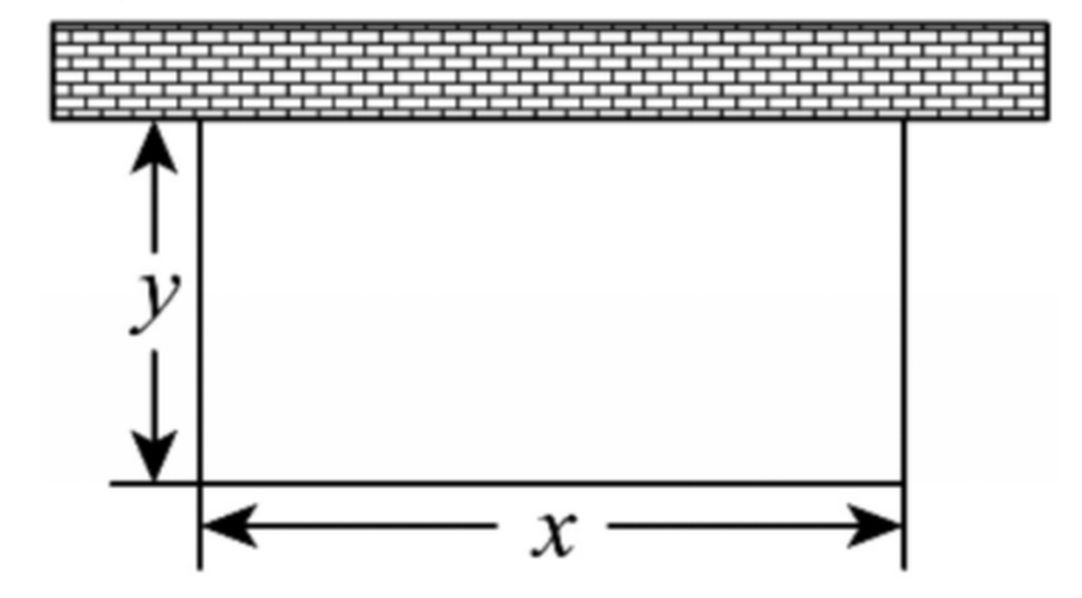
\includegraphics[width=0.42\textwidth]{figures/gao142_q20.png}
\end{center}

(1) 若菜园面积为 72 平方米，则 $x$、$y$ 为何值时，所用篱笆总长最小？

(2) 若 $x$、$y$ 满足 $x+y-xy+63=0$，则菜园面积最小为多少平方米？

\ifanswer
\solbegin
\step{(1) 由题意得，菜园的面积 $S=xy=72$，且 $x>0$，$y>0$，}
\step{所用篱笆总长 $L=x+2y$，}
\step{由基本不等式得 $x+2y\geqslant2\sqrt{x\cdot2y}=2\sqrt{2xy}=2\sqrt{2\times72}=24$，}
\step{当且仅当 $x=2y$ 时取等号，}
\step{联立 $\begin{cases}xy=72\\x=2y\end{cases}$，解得 $\begin{cases}x=12\\y=6\end{cases}$，}
\step{所以当 $x=12$，$y=6$ 时，所用篱笆总长最小；}
\step{(2) 由题意得 $x>0$，$y>0$，且满足 $x+y-xy+63=0$，即 $x+y=xy-63$，}
\step{由基本不等式得 $x+y\geqslant2\sqrt{xy}$，当且仅当 $x=y$ 时取等号，}
\step{所以 $xy-63\geqslant2\sqrt{xy}$. 令 $t=\sqrt{xy}(t>0)$，则 $xy=t^2$，}
\step{上述不等式可化为 $t^2-2t-63\geqslant0$，即 $(t-9)(t+7)\geqslant0$，}
\step{因为 $t>0$，所以 $t+7>0$，故 $t-9\geqslant0$，解得 $t\geqslant9$，所以 $\sqrt{xy}\geqslant9$，}
\step{即 $xy\geqslant81$，当且仅当 $x=y=9$ 时取等号，此时满足 $9+9-81+63=0$，}
\step{所以菜园面积最小为 81 平方米.}
\solend
\fi

\item 已知幂函数 $f(x)=(m^2-3m+3)x^m$ 的图象关于 $y$ 轴对称.

(1) 求实数 $m$ 的值；

(2) 在平面直角坐标系中作出函数 $y=\lvert f(x)-1\rvert$ 的图象；

(3) 已知点 $A(2a,y_1)$ 与点 $B(3-a,y_2)$ 都在幂函数 $y=x^2$ 的图象上. 若 $y_1<y_2$，求实数 $a$ 的取值范围.

\begin{center}
% 空白坐标网格取原卷 08 页截图去粉色水印、去色、LANCZOS 放大；题目配图，三版都出
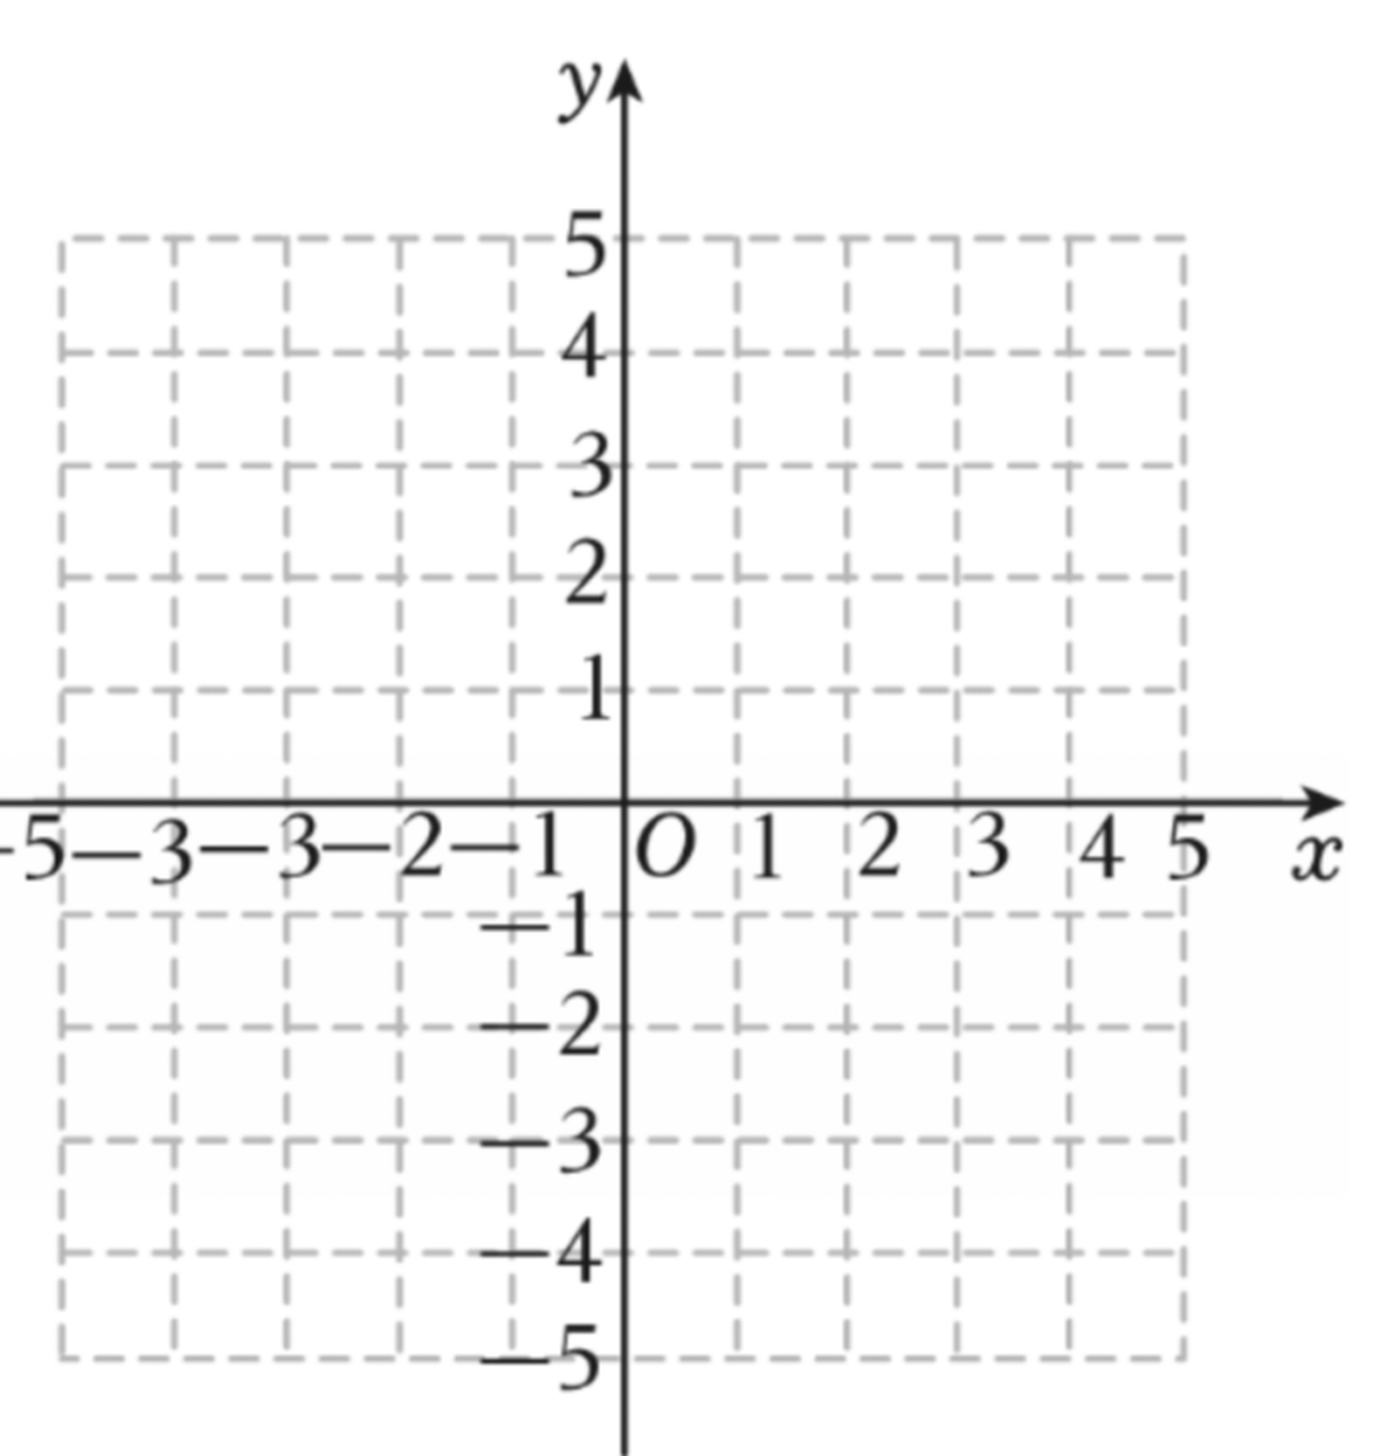
\includegraphics[width=0.52\textwidth]{figures/gao142_q21_grid.png}
\end{center}

\ifanswer
\solbegin
\step{(1) 由题意幂函数 $f(x)=(m^2-3m+3)x^m$，}
\step{故 $m^2-3m+3=1$，解得 $m=1$ 或 $m=2$，}
\step{又 $f(x)$ 图象关于 $y$ 轴对称，即 $f(x)$ 是偶函数，}
\step{当 $m=1$ 时，$f(x)=x$ 是奇函数，不满足条件，舍去；}
\step{当 $m=2$ 时，$f(x)=x^2$ 是偶函数，满足条件，故 $m=2$；}
\step{(2) 由 (1) 得，$\lvert f(x)-1\rvert=\lvert x^2-1\rvert$，}
\step{先画 $y=x^2-1$，开口向上的抛物线，顶点 $(0,-1)$，零点 $x=\pm1$，}
\step{再将 $x$ 轴下方的部分沿 $x$ 轴翻折到上方即为 $y=\lvert x^2-1\rvert$ 的图象，}
\step{图象如图所示.}
\par{\leftskip=0pt
\begin{center}
% 抛物线图象取原卷 09 页截图去粉色水印、去色、LANCZOS 放大；解析所附配图，仅答案版出
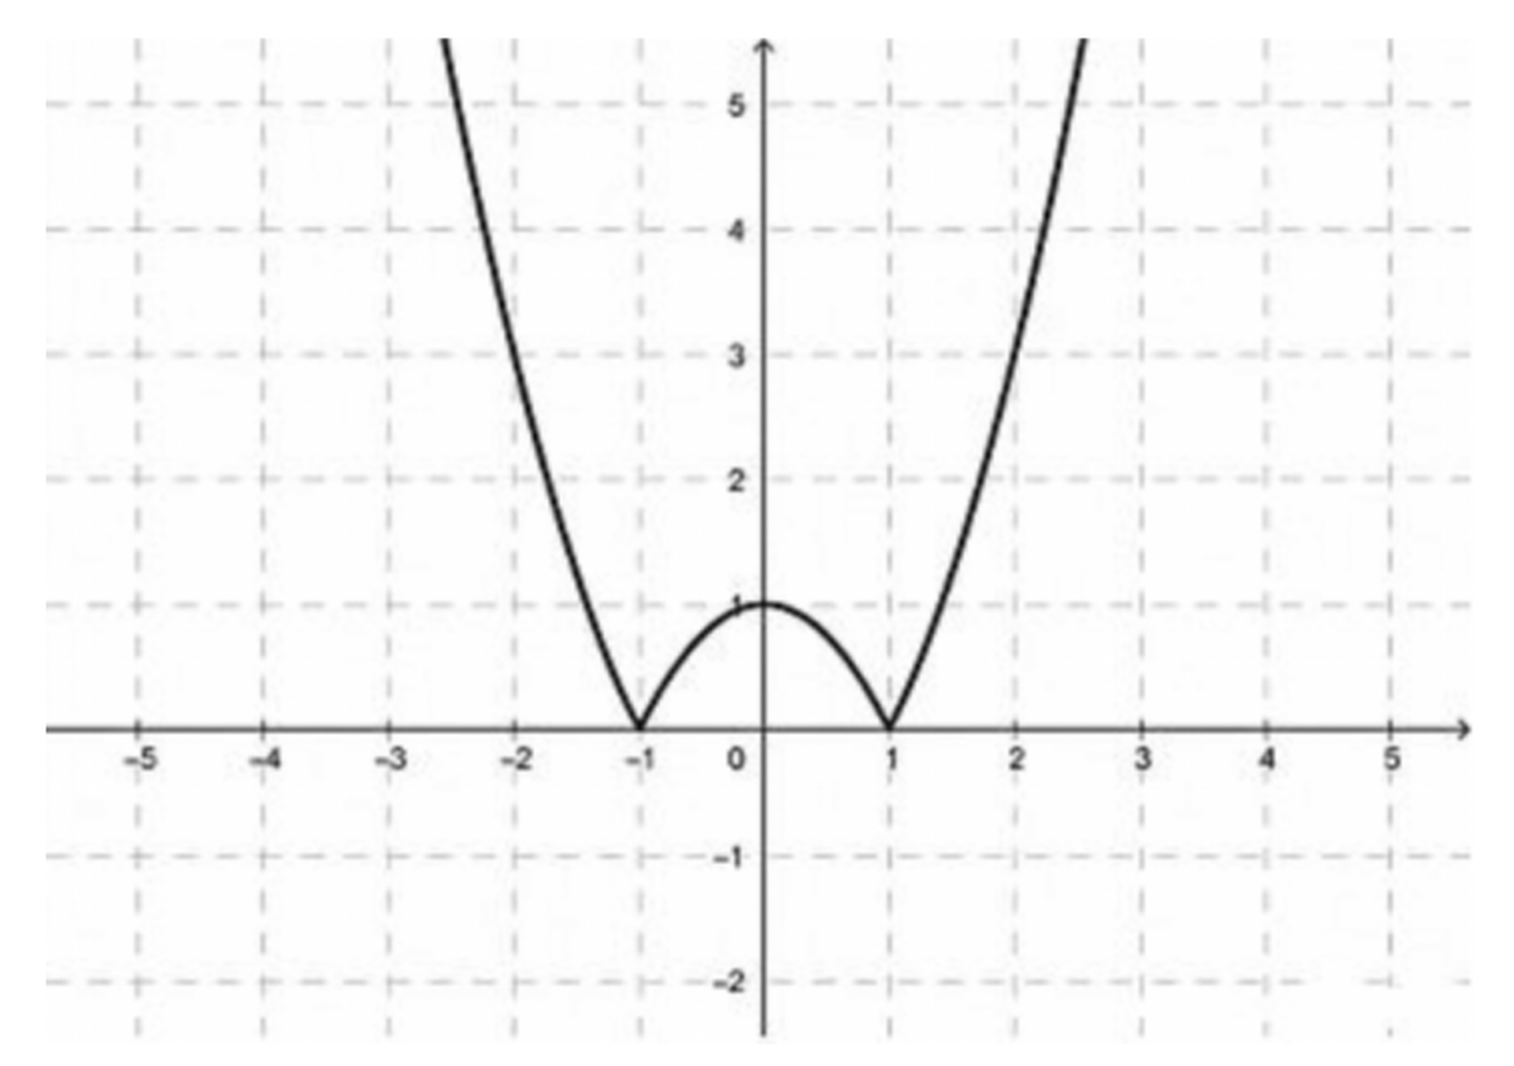
\includegraphics[width=0.55\textwidth]{figures/gao142_q21_para.png}
\end{center}}
\step{(3) 由题意得，$y_1=(2a)^2$，$y_2=(3-a)^2$，}
\step{$y_1<y_2$，即有 $(2a)^2<(3-a)^2$，化简整理得 $(a+3)(a-1)<0$，}
\step{解得实数 $a$ 的取值范围为 $(-3,1)$.}
\solend
\fi

\end{enumerate}

\end{document}
"
% 紧凑版：xelatex "\def\iscompact{1}% 高一142_群峰高级中学_期中.tex
%   —— 高一上数学"2026-2027 年群峰高级中学高一上期中"（试卷版/答案版）
% 试卷版：xelatex 高一142_群峰高级中学_期中.tex
% 答案版：xelatex "\def\isanswer{1}\input{高一142_群峰高级中学_期中.tex}"
% 紧凑版：xelatex "\def\iscompact{1}\input{高一142_群峰高级中学_期中.tex}"
%
% ① 原始材料：微信公众号"魔都数学加油站"文章，连载"27学年高一142"，原文标题
% "27学年高一142——2026-2027年上海市群峰高级中学高一上期中"；
% 原文链接：https://mp.weixin.qq.com/s/cc7wnuP4Pk3OjNDV6ihB9A。
% 正文为 9 张 PNG 页（01、02、04、06、07、08、09 为 2560x3620；03、05 为 4762x6735，
% 同一篇各页分辨率不同，逐页按各自分辨率裁图核对），题目下印有【答案】或【解析】，为讲评版。
% 题目、解析均据原图转录；卷面粉红色水印"魔都数学加油站"及公众号页脚未录入。
% 全卷 4 幅插图：第 15 题四幅坐标函数图像选项（04 页，2x2 合并为一张）、
% 第 20 题矩形围栏示意图（07 页）、第 21 题 (2) 空白坐标网格（08 页）、
% 第 21 题抛物线图象（09 页，解析所附图）；均取原卷截图去粉色水印、LANCZOS 放大。
% 题目配图三版都出、解析配图仅答案版出。
%
% 卷首标题：原卷印作"2026-2027 年群峰高级中学高一上期中"（公众号标题中的"上海市"
% 卷面标题行没有，本稿照卷面），年份区间按全稿惯例排 en dash；原卷未印副标题，
% 本卷为期中卷、跨集合与常用逻辑用语／不等式／函数三章，按题目内容补出
% "集合与常用逻辑用语、不等式、函数"（头注说明，与同期中卷口径相同）。
%
% 题号体例：本卷共 19 题——一、填空题 3—12（10 题）、二、选择题 13—16（4 题）、
% 三、解答题 17—21（5 题）。三节分别 \setcounter{enumi}{2}／{12}／{16}。
% 原卷从第 3 题起、无第 1、2 题，本稿保留原题号。
%
% ② 与原卷的排版差异：
%   ① 原文从第 3 题起，本稿保留原题号；原卷未印副标题，本稿按"知识模块"口径补出；
%   ② 逐题答案口径：Q14 原卷把答案 D 印在题干括号内、且题目下无【解析】，本稿括号
%      留空 \mbox{（\quad）}、另提 \ans{D}；Q13／Q15／Q16 答案在【解析】末句"故选 …"
%      （分别为 C／C／A），题干括号留空、不另提 \ans{}；其余各题（Q3—Q12、
%      Q17—Q21）题目下印【解析】、答案融在解析中，不另提 \ans{}；全卷仅 Q14 一处 \ans{}；
%      答案版【答案】/【解析】标记数 = 19（1 个 \ans + 18 个 \solbegin）= 全卷题数；
%   ③ 原卷填空横线按全稿惯例排 \blankline[4.4em]；选择题括号排 \mbox{（\quad）}、
%      每个选项段前按惯例加 \keepwithprev（Q15 四幅图那一枚放在 \begin{center} 之前）；
%      解答题不留作答区、不加 \anspace（原卷为讲评版，与 129／131／132／133／136／140 同）；
%   ④ 原卷数集斜体 $R$（Q5、Q7、Q19、Q21 解析等）按全稿惯例统一改 \R；空集记号
%      \varnothing；绝对值排 \lvert…\rvert，集合描述竖线排 \mid；不等号按全稿惯例
%      排 \leqslant／\geqslant；
%   ⑤ 4 幅插图：Q15 四幅坐标函数图象选项合并裁为一张 \includegraphics（题前
%      \needvspace{9cm}）；Q15 是"二、选择题"节内带大图块的第 3 题（Q13、Q14 在前
%      且无图），另在 \bigsec{二、选择题} 之前加 \needvspace{11cm} 连节标题一起量
%      ——守卫必须放在 \bigsec 之前，放标题之后会让"二、选择题"孤立在页末
%      （B 类，照 高一26／40／59／136／140 成例）；Q20 围栏图与 Q21 网格图置于题干
%      之后（三版都出），Q21 抛物线图置于答案版解析 (2) 与 (3) 之间（仅答案版出）；
%   ⑥ 子题标号按原卷排半角 (1)(2)(3)（与 140／141 同期中卷口径相同）；括注全角／
%      半角逐处照录：Q3"（用含有 m 的代数式表示）"、Q6"（舍）"、Q10"（万元）"、
%      Q18"（请务必书写必要的计算步骤）"、Q20"（墙足够长）"印全角；Q15
%      "$y=a^x(a>0 且 a\neq1)$"、Q10"$y=x^a(a 为常数)$"、Q20"$t=\sqrt{xy}(t>0)$"
%      等数学式内括注印半角；数学式内 CJK 用 \text{…}（否则 FONTCHK 报缺字）；
%   ⑦ 数学式内半角逗号照录（如 Q6"$ax-1=0,a\in\R$"、Q9"$b=2+\sqrt2,a=\sqrt2+1$"、
%      Q16 区间 "$[-1,3]$"、Q21"$y_1<y_2$，即 $(2a)^2<(3-a)^2$" 等）；原卷行末
%      西文句点照录（Q7"(-3,5)."、Q10"125（万元）."、Q19 题干句点、Q20 题干
%      "矩形菜园."与"宽为 y 米."、Q21 题干"对称." 等）；行中全角逗号、分号照录；
%   ⑧ 题干中的中文弯引号：本卷题干与解析通篇未出现中文弯引号，故无此项；
%      圈数字 ①②③ 亦未出现（子题用 (1)(2)(3)）；
%   ⑨ 原卷"图像／图象"两种写法混用，逐处放大核对并照录：Q4 题干与解析作"图象"、
%      Q7 解析作"图象"、Q8 题干作"图像"而解析作"图象"、Q15 题干与解析通篇作
%      "图像"、Q21 题干与解析通篇作"图象"；
%   ⑩ 原卷无红色加粗标签（【解析】均黑色印刷；逐页扫描深红像素为 0），故本卷未用
%      \stepm；黑色常规分步标签（"A 中""C 中""D 中""(1)(2)(3)" 等）按普通 \step
%      行内文字照录；
%   ⑪ 跨页续印按题合并，明细见 ⑥。
%
% ③ 行数复核：一条 \step = 原卷解析的一个印刷行，cases 块作一个印刷行计。逐题数 \step
%   条数，合计 98 条（Q3：1；Q4：2；Q5：3；Q6：4；Q7：5；Q8：2；Q9：4；Q10：3；
%   Q11：4；Q12：3；Q13：5；Q14：0；Q15：10；Q16：4；Q17：10；Q18：3；
%   Q19：10；Q20：13；Q21：12），与原卷印刷行逐题相等。Q14 只把答案印在题干括号、
%   无【解析】，提 \ans{D}、不计入 \step 账；答案版标记数 = 19（1 个 \ans + 18 个
%   \solbegin）= 全卷题数。
%
% ④ 判别式字形：全卷判别式共 3 处——第 7 题【解析】"即判别式△<0"、
%   "即△=(a-1)^2-4×1×4<0" 两处原卷印扁等边三角 $\triangle$，
%   第 11 题【解析】cases 块"△=4a^2-4(a+6)≥0" 一处原卷印等腰偏高的高三角 $\Delta$；
%   逐处放大核对，两形不同、全卷混用，本稿逐处照录不统一（参照 高一141 头注④口径）。
%   子集符号：全卷共 3 处——第 6 题题干"若 B⊆A"、第 6 题【解析】"因为 B⊆A"、
%   第 17 题【解析】(2)"所以 A⊆B"，逐处放大核对，原卷三处均印带下划线的
%   $\subseteq$（不是单线 $\subset$），本稿一律照录 \subseteq；全卷未出现 \subset。
%
% ⑤ 原卷存疑照录（均照录未改，正文对应处另有 % 注）：
%   第 14 题题干括号内原卷印答案 D（非留空），且题目下无【解析】，按"答案印括号且
%      无解析"口径括号留空、另提 \ans{D}；
%   第 15 题【解析】"C 中，由指数函数 … 图像递减得 a>1" 中"递减"与"a>1"
%      自相矛盾（递减应得 0<a<1，疑为"递增"之误），照录；
%   第 16 题选项 B 作 $(-\infty,3]\cup[3,+\infty)$，两端区间并起即全体实数、
%      与正确答案 $[-1,3]$ 不成干扰项（疑为 $(-\infty,-1]\cup[3,+\infty)$ 之误），照录；
%   第 21 题 (2) 空白坐标网格的 x 轴刻度原卷印作"-5 -3 -3 -2 -1 0 1 2 3 4 5"
%      （"-3"重复，疑为"-4"之误），系插图中的印刷内容，取原卷截图照录、不改图。
%
% ⑥ 跨页续印说明：Q7 题干与解析首行在 01 页、解析续至 02 页；Q11 题干与解析
%   4 行在 03 页；Q13 解析前 4 行在 03 页、末句"故选 C."续至 04 页；Q15 题干与
%   四幅图在 04 页、解析前 8 行在 04 页、末 2 行续至 05 页；Q17 解析前 7 行在
%   05 页、后 3 行续至 06 页；Q19 解析前 5 行在 06 页、后 5 行续至 07 页；
%   Q20 解析前 9 行在 07 页、后 4 行续至 08 页；Q21 解析 (1)(2) 9 行在 08 页、
%   抛物线图与 (3) 3 行续至 09 页；本稿按题连排，不丢行。三版切页审计结论见
%   编译自验回报（切页守卫见 ②⑤）。
%
\documentclass[a4paper,11pt]{article}
\usepackage{common}

\begin{document}

\examtitlest[3]{2026--2027 年群峰高级中学高一上期中}{集合与常用逻辑用语、不等式、函数}

\bigsec{一、填空题}

\begin{enumerate}
\setcounter{enumi}{2}

\item 已知 $\log_2 3=m$，则 $\log_3 6=$\blankline[4.4em]（用含有 $m$ 的代数式表示）.

\ifanswer
\solbegin
\step{$\log_3 6=\dfrac{\log_2 6}{\log_2 3}=\dfrac{\log_2 2+\log_2 3}{\log_2 3}=\dfrac{1+m}{m}=\dfrac1m+1$.}
\solend
\fi

\item 若指数函数 $y=a^x$ 的图象经过点 $(3,27)$，则 $a$ 的值为\blankline[4.4em].

\ifanswer
\solbegin
\step{因为指数函数 $y=a^x$ 的图象经过点 $(3,27)$，}
\step{所以 $a^3=27=3^3$，所以 $a=3$.}
\solend
\fi

\item 不等式 $(2x+1)^{\frac13}<(3-x)^{\frac13}$ 的解集为\blankline[4.4em].

\ifanswer
\solbegin
\step{因为幂函数 $f(t)=t^{\frac13}$ 在 $\R$ 上严格增，}
\step{所以原不等式等价于 $2x+1<3-x$，解得 $x<\dfrac23$，}
\step{因此原不等式的解集为 $\left(-\infty,\dfrac23\right)$.}
\solend
\fi

\item 设集合 $A=\{1,-2\}$，$B=\{x\mid ax-1=0,a\in\R\}$，若 $B\subseteq A$，则 $a$ 的值为\blankline[4.4em].% 子集符号原卷印带下划线 $\subseteq$，照录

\ifanswer
\solbegin
\step{因为 $B\subseteq A$，所以 $B=\varnothing$ 或 $\{-2\}$ 或 $\{1\}$ 或 $\{1,-2\}$（舍），}% 子集符号原卷印带下划线 $\subseteq$，照录
\step{若 $B=\varnothing$，则 $a=0$；若 $B=\{1\}$，则 $a=1$；}
\step{若 $B=\{-2\}$，则 $-2a=1$，解得 $a=-\dfrac12$；}
\step{综上，$a=0$ 或 $1$ 或 $-\dfrac12$.}
\solend
\fi

\item 不等式 $x^2+(a-1)x+4>0$ 在 $\R$ 上恒成立，则实数 $a$ 的取值范围是\blankline[4.4em].

\ifanswer
\solbegin
\step{不等式 $x^2+(a-1)x+4>0$，对应的二次函数为 $y=x^2+(a-1)x+4$，}
\step{因此函数图象开口向上，要使不等式对任意实数 $x$ 恒成立，}
\step{需二次函数图象与 $x$ 轴无交点，即判别式 $\triangle<0$，}% 判别式原卷印扁等边三角 $\triangle$，照录
\step{即 $\triangle=(a-1)^2-4\times1\times4<0$，整理得 $a^2-2a-15<0$，}% 判别式原卷印扁等边三角 $\triangle$，照录
\step{解得 $-3<a<5$，故实数 $a$ 的取值范围是 $(-3,5)$.}
\solend
\fi

\item 函数 $f(x)=(5x-3)^a$ 的图像恒过点\blankline[4.4em].% 题干作"图像"、解析作"图象"，原卷混用，逐处照录

\ifanswer
\solbegin
\step{令 $5x-3=1$ 得 $x=\dfrac45$，此时 $f\left(\dfrac45\right)=\left(5\times\dfrac45-3\right)^a=1$，}
\step{所以 $f(x)$ 的图象恒过 $\left(\dfrac45,1\right)$.}
\solend
\fi

\item 若 $a>0$，$b>0$ 且 $\dfrac1a+\dfrac2b=1$，则 $a+b$ 的最小值为\blankline[4.4em].

\ifanswer
\solbegin
\step{因为 $a>0$，$b>0$，$\dfrac1a+\dfrac2b=1$，}
\step{所以 $a+b=(a+b)\left(\dfrac1a+\dfrac2b\right)=1+\dfrac{2a}{b}+\dfrac{b}{a}+2\geqslant3+2\sqrt{\dfrac{2a}{b}\cdot\dfrac{b}{a}}=3+2\sqrt2$，}
\step{当且仅当 $\dfrac{2a}{b}=\dfrac{b}{a}$，即 $b=2+\sqrt2,a=\sqrt2+1$ 时取等号，}
\step{故 $a+b$ 的最小值为 $3+2\sqrt2$.}
\solend
\fi

\item 某药厂研制出一种新型药剂，投放市场后其广告投入 $x$（万元）与药品利润 $y$（万元）存在的关系为 $y=x^a(a\text{ 为常数})$，其中 $x$ 不超过 5 万元. 已知去年投入广告费用为 3 万元时，药品利润为 27 万元，若今年投入广告费用 5 万元，预计今年药品利润为\blankline[4.4em]万元.

\ifanswer
\solbegin
\step{由已知投入广告费用为 3 万元时，药品利润为 27 万元，}
\step{代入 $y=x^a$ 中，即 $3^a=27$，解得 $a=3$，故函数关系式为 $y=x^3$，}
\step{所以当 $x=5$ 时，$y=125$（万元）.}
\solend
\fi

\item 已知方程 $x^2+2ax+a+6=0$ 的两根分别是 $x_1$ 和 $x_2$，且满足 $\dfrac1{x_1}+\dfrac1{x_2}<0$，则实数 $a$ 的取值范围是\blankline[4.4em].

\ifanswer
\solbegin
\step{由于方程 $x^2+2ax+a+6=0$ 的两根分别是 $x_1$ 和 $x_2$，}
\step{则 $\begin{cases}\Delta=4a^2-4(a+6)\geqslant0\\x_1+x_2=-2a\\x_1x_2=a+6\end{cases}$，解得 $a\geqslant3$ 或 $a\leqslant-2$.}% 判别式原卷印等腰偏高的高三角 $\Delta$，照录（与第 7 题扁等边 $\triangle$ 两形混用）
\step{又 $\dfrac1{x_1}+\dfrac1{x_2}<0$，即 $\dfrac{x_1+x_2}{x_1\cdot x_2}<0$，故 $\dfrac{-2a}{a+6}<0$，解得 $a<-6$ 或 $a>0$.}
\step{综上，$a$ 的取值范围是 $(-\infty,-6)\cup[3,+\infty)$.}
\solend
\fi

\item 已知 $b>a>1$，若 $\log_a b-\log_b a=\dfrac32$，$a^b=b^a$，则 $a-b=$\blankline[4.4em].

\ifanswer
\solbegin
\step{因为 $b>a>1$，所以 $\log_a b>1$，}
\step{由 $\log_a b-\log_b a=\log_a b-\dfrac{1}{\log_a b}=\dfrac32$，解得 $\log_a b=2$ 即 $b=a^2$，}
\step{因为 $a^b=b^a=a^{2a}$，所以 $b=2a=a^2$，所以 $a=2$，$b=4$，则 $a-b=-2$.}
\solend
\fi

\end{enumerate}

% 第 15 题四幅图是"二、选择题"节内的大图块；守卫须放在 \bigsec 之前连节标题一起量
\needvspace{11cm}
\bigsec{二、选择题}

\begin{enumerate}
\setcounter{enumi}{12}

\item 若 $a>b$，$c<0$，则下列不等式正确的是\mbox{（\quad）}

\keepwithprev
A. $ab>bc$\qquad B. $a+c<b+c$\qquad C. $ac^2>bc^2$\qquad D. $\dfrac ac>\dfrac bc$

\ifanswer
\solbegin
\step{因为 $a>b$，$c<0$，取 $b=0$，则 $ab=bc=0$，故 $A$ 错误；}
\step{由于 $a>b$，所以 $a+c>b+c$，故 $B$ 错误；}
\step{由 $c<0$ 得 $c^2>0$，所以 $ac^2>bc^2$，故 $C$ 正确；}
\step{由于 $a>b$ 且 $c<0$，所以 $\dfrac ac<\dfrac bc$，故 $D$ 错误.}
\step{故选 $C$.}
\solend
\fi

\item 若 $x>0$，$y>0$，则下列各式中，恒成立的是\mbox{（\quad）}% 原卷题干括号内印答案 D、且题目下无【解析】，本稿括号留空、另提 \ans{D}

\keepwithprev
A. $\lg x+\lg y=\lg(x+y)$\qquad B. $\lg x^2=(\lg x)^2$

C. $\dfrac{\lg x}{\lg y}=\lg(x-y)$\qquad D. $\lg x^{\frac1n}=\dfrac{\lg x}{n}$

\ifanswer
\ans{$D$}
\fi

% 第 15 题四幅坐标函数图象选项是一整块，守卫放在 \item 之前
\needvspace{9cm}
\item 在同一平面直角坐标系中，指数函数 $y=a^x(a>0\text{ 且 }a\neq1)$ 和一次函数 $y=a(x+1)$ 的图像关系可能是\mbox{（\quad）}

\keepwithprev
\begin{center}
% 四幅坐标函数图象选项取原卷 04 页截图去粉色水印、去色，按原卷 2x2 排布合并为一张
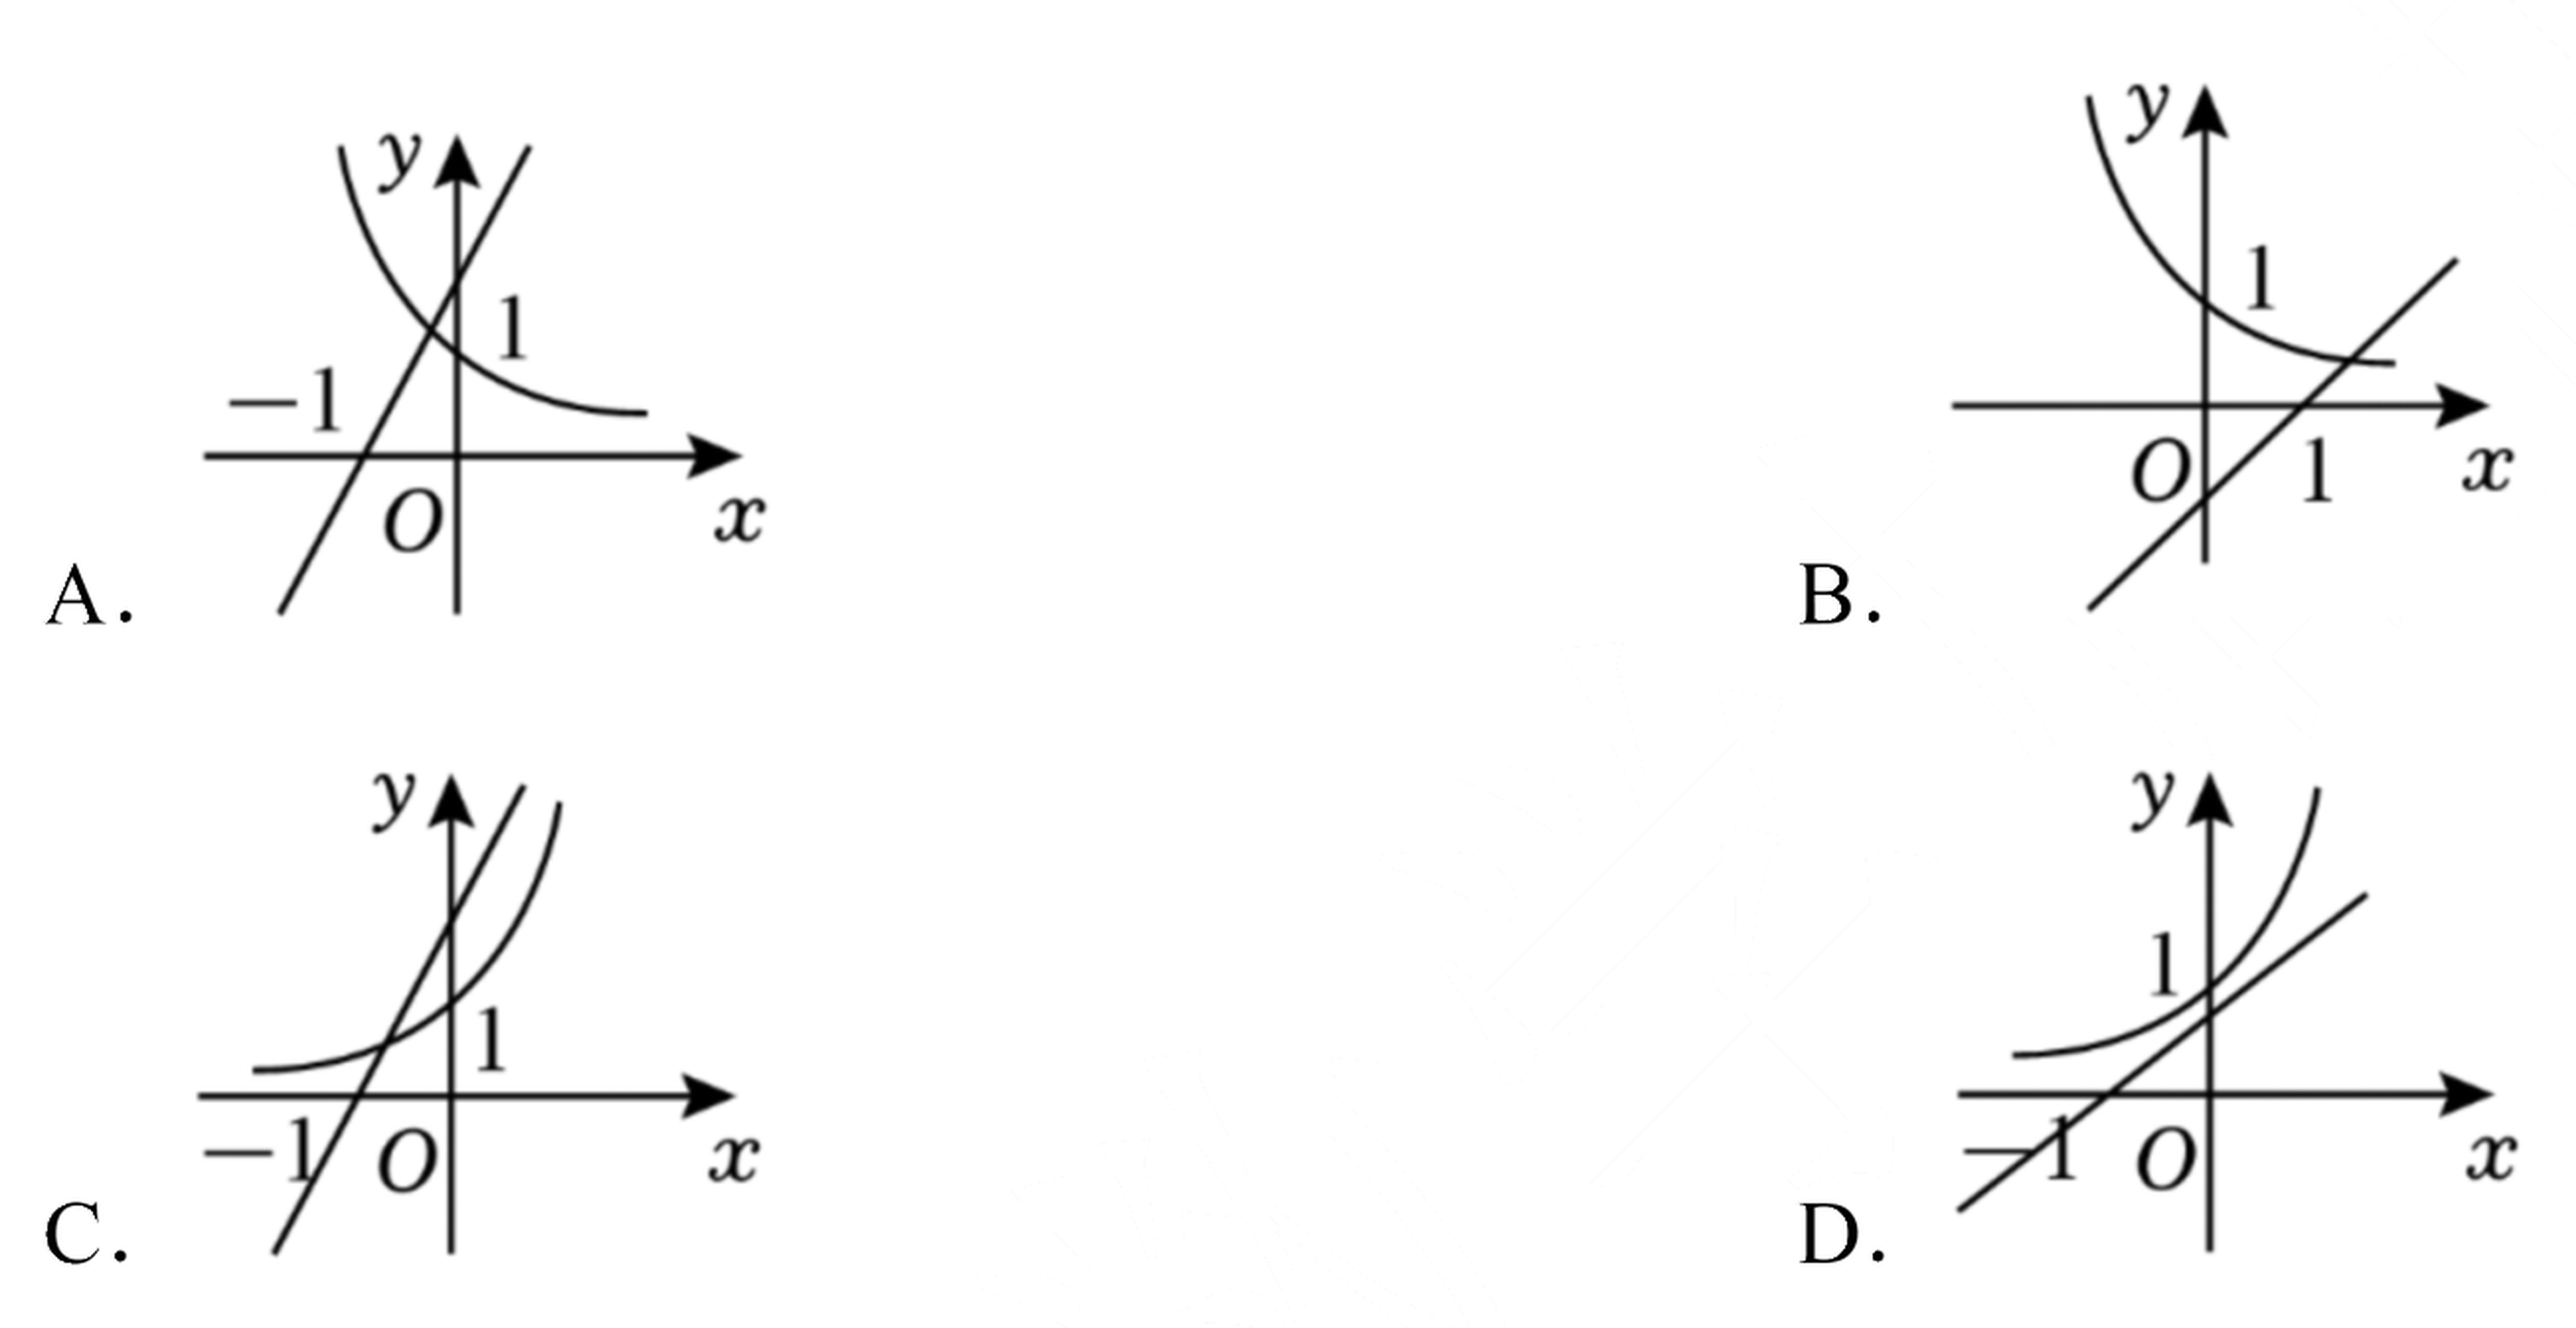
\includegraphics[width=0.80\textwidth]{figures/gao142_q15.png}
\end{center}

\ifanswer
\solbegin
\step{$A$ 中，由指数函数 $y=a^x(a>0\text{ 且 }a\neq1)$ 图像递减得 $0<a<1$，}
\step{而一次函数 $y=a(x+1)$ 的图像与 $y$ 轴交点纵坐标为 $a>1$，二者矛盾，}
\step{所以 $A$ 错；}
\step{由一次函数 $y=a(x+1)$ 的图像与 $x$ 轴交点横坐标为 $-1$，排除 $B$；}
\step{$C$ 中，由指数函数 $y=a^x(a>0\text{ 且 }a\neq1)$ 图像递减得 $a>1$，}% 原卷"递减得 a>1"自相矛盾（递减应得 0<a<1），照录
\step{而一次函数 $y=a(x+1)$ 的图像与 $y$ 轴交点纵坐标为 $a>1$，二者 $a$ 值吻合，}
\step{所以 $C$ 对；}
\step{$D$ 中，由一次函数 $y=a(x+1)$ 的图像得 $a=1$，与 $a>0$ 且 $a\neq1$ 矛盾，}
\step{所以 $D$ 错.}
\step{故选 $C$.}
\solend
\fi

\item 不等式 $\lvert x+1\rvert+\lvert 2-x\rvert\geqslant a^2-2a$ 恒成立，则 $a$ 的取值范围是\mbox{（\quad）}

\keepwithprev
A. $[-1,3]$\qquad B. $(-\infty,3]\cup[3,+\infty)$\qquad C. $(-\infty,3)$\qquad D. $(3,+\infty)$

\ifanswer
\solbegin
\step{因为 $\lvert x+1\rvert+\lvert 2-x\rvert\geqslant\lvert(x+1)+(2-x)\rvert=3$，}
\step{所以 $\lvert x+1\rvert+\lvert 2-x\rvert$ 的最小值为 3，}
\step{因为 $\lvert x+1\rvert+\lvert 2-x\rvert\geqslant a^2-2a$ 恒成立，所以只需 $a^2-2a\leqslant3$，所以 $-1\leqslant a\leqslant3$，}
\step{所以 $a$ 的取值范围为 $[-1,3]$. 故选 $A$.}
\solend
\fi

\end{enumerate}

\bigsec{三、解答题}

\begin{enumerate}
\setcounter{enumi}{16}

\item 已知集合 $A=\left\{x\mid\dfrac{x-3}{x-1}\leqslant0\right\}$，$B=\{x\mid\lvert x-1\rvert<a\}$.

(1) 若 $a=1$，求 $A\cap B$；

(2) 若 $x\in A$ 是 $x\in B$ 的充分条件，求 $a$ 的取值范围.

\ifanswer
\solbegin
\step{(1) 不等式 $\dfrac{x-3}{x-1}\leqslant0$，等价于 $(x-3)(x-1)\leqslant0$ 且 $x-1\neq0$，解得 $1<x\leqslant3$，}
\step{所以 $A=\{x\mid 1<x\leqslant3\}$，}
\step{当 $a=1$ 时，不等式 $\lvert x-1\rvert<a$ 可化为 $\lvert x-1\rvert<1$，所以 $-1<x-1<1$，}
\step{故 $0<x<2$，所以 $B=\{x\mid 0<x<2\}$，}
\step{所以 $A\cap B=\{x\mid 1<x<2\}$；}
\step{(2) 因为 $x\in A$ 是 $x\in B$ 的充分条件，所以 $A\subseteq B$，}% 子集符号原卷印带下划线 $\subseteq$，照录
\step{因为 $A=\{x\mid 1<x\leqslant3\}\neq\varnothing$，所以 $B\neq\varnothing$，故 $a>0$，}
\step{由不等式 $\lvert x-1\rvert<a$，解得 $1-a<x<1+a$，}
\step{所以 $B=\{x\mid 1-a<x<1+a\}$，所以 $\begin{cases}1-a\leqslant1\\1+a>3\end{cases}$，解得 $a>2$，}
\step{所以 $a$ 的取值范围为 $(2,+\infty)$.}
\solend
\fi

\item 计算下列式子的值（请务必书写必要的计算步骤）

(1) $27^{\frac13}+\left(\dfrac76\right)^0+\sqrt{(3-\pi)^2}$；

(2) $\lg25+\lg4+7^{\log_7 2}-\log_2 3\times\log_3 4+\log_3 9$.

\ifanswer
\solbegin
\step{(1) $27^{\frac13}+\left(\dfrac76\right)^0+\sqrt{(3-\pi)^2}=3^{3\times\frac13}+1+\lvert 3-\pi\rvert=3+1+\pi-3=\pi+1$；}
\step{(2) 原式 $=\lg(25\times4)+2-\dfrac{\lg3}{\lg2}\times\dfrac{\lg4}{\lg3}+2=\lg100+2-\dfrac{2\lg2}{\lg2}+2$}
\step{$=2+2-2+2=4$.}
\solend
\fi

\item 已知关于 $x$ 的不等式 $mx^2-(3m^2-m+2)x+6m-2\geqslant0$.

(1) 当 $m=2$ 时，求关于 $x$ 的不等式的解集；

(2) 当 $m>0$ 时，求关于 $x$ 的不等式的解集.

\ifanswer
\solbegin
\step{(1) $m=2$ 时，不等式为 $x^2-6x+5\geqslant0$，即 $(x-1)(x-5)\geqslant0$，}
\step{解得 $x\leqslant1$ 或 $x\geqslant5$，所以不等式的解集是 $\{x\mid x\leqslant1$ 或 $x\geqslant5\}$.}
\step{(2) $m>0$ 时，不等式可化为 $(mx-2)[x-(3m-1)]\geqslant0$，}
\step{即 $\left(x-\dfrac2m\right)[x-(3m-1)]\geqslant0$，}
\step{若 $m=1$，则不等式为 $(x-2)^2\geqslant0$，解得 $x\in\R$；}
\step{若 $0<m<1$，则 $\dfrac2m>3m-1$，解不等式得 $x\geqslant\dfrac2m$ 或 $x\leqslant3m-1$；}
\step{若 $m>1$，则 $\dfrac2m<3m-1$，解不等式得 $x\geqslant3m-1$ 或 $x\leqslant\dfrac2m$；}
\step{综上，$0<m<1$ 时，不等式的解集是 $\{x\mid x\leqslant3m-1$ 或 $x\geqslant\dfrac2m\}$；}
\step{$m=1$ 时，不等式的解集为 $\R$；}
\step{$m>1$ 时，不等式的解集是 $\{x\mid x\leqslant\dfrac2m$ 或 $x\geqslant3m-1\}$.}
\solend
\fi

\item 如图，某人计划用篱笆围成一个一边靠墙（墙足够长）的矩形菜园. 设菜园的长为 $x$ 米，宽为 $y$ 米.

\begin{center}
% 矩形围栏示意图取原卷 07 页截图去粉色水印、去色、LANCZOS 放大；题目配图，三版都出
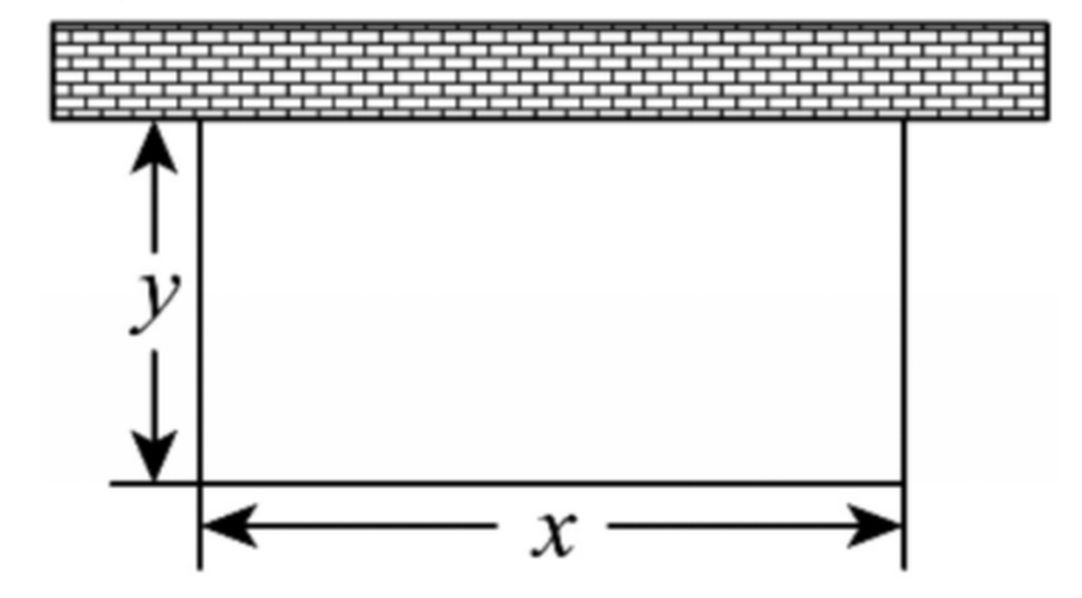
\includegraphics[width=0.42\textwidth]{figures/gao142_q20.png}
\end{center}

(1) 若菜园面积为 72 平方米，则 $x$、$y$ 为何值时，所用篱笆总长最小？

(2) 若 $x$、$y$ 满足 $x+y-xy+63=0$，则菜园面积最小为多少平方米？

\ifanswer
\solbegin
\step{(1) 由题意得，菜园的面积 $S=xy=72$，且 $x>0$，$y>0$，}
\step{所用篱笆总长 $L=x+2y$，}
\step{由基本不等式得 $x+2y\geqslant2\sqrt{x\cdot2y}=2\sqrt{2xy}=2\sqrt{2\times72}=24$，}
\step{当且仅当 $x=2y$ 时取等号，}
\step{联立 $\begin{cases}xy=72\\x=2y\end{cases}$，解得 $\begin{cases}x=12\\y=6\end{cases}$，}
\step{所以当 $x=12$，$y=6$ 时，所用篱笆总长最小；}
\step{(2) 由题意得 $x>0$，$y>0$，且满足 $x+y-xy+63=0$，即 $x+y=xy-63$，}
\step{由基本不等式得 $x+y\geqslant2\sqrt{xy}$，当且仅当 $x=y$ 时取等号，}
\step{所以 $xy-63\geqslant2\sqrt{xy}$. 令 $t=\sqrt{xy}(t>0)$，则 $xy=t^2$，}
\step{上述不等式可化为 $t^2-2t-63\geqslant0$，即 $(t-9)(t+7)\geqslant0$，}
\step{因为 $t>0$，所以 $t+7>0$，故 $t-9\geqslant0$，解得 $t\geqslant9$，所以 $\sqrt{xy}\geqslant9$，}
\step{即 $xy\geqslant81$，当且仅当 $x=y=9$ 时取等号，此时满足 $9+9-81+63=0$，}
\step{所以菜园面积最小为 81 平方米.}
\solend
\fi

\item 已知幂函数 $f(x)=(m^2-3m+3)x^m$ 的图象关于 $y$ 轴对称.

(1) 求实数 $m$ 的值；

(2) 在平面直角坐标系中作出函数 $y=\lvert f(x)-1\rvert$ 的图象；

(3) 已知点 $A(2a,y_1)$ 与点 $B(3-a,y_2)$ 都在幂函数 $y=x^2$ 的图象上. 若 $y_1<y_2$，求实数 $a$ 的取值范围.

\begin{center}
% 空白坐标网格取原卷 08 页截图去粉色水印、去色、LANCZOS 放大；题目配图，三版都出
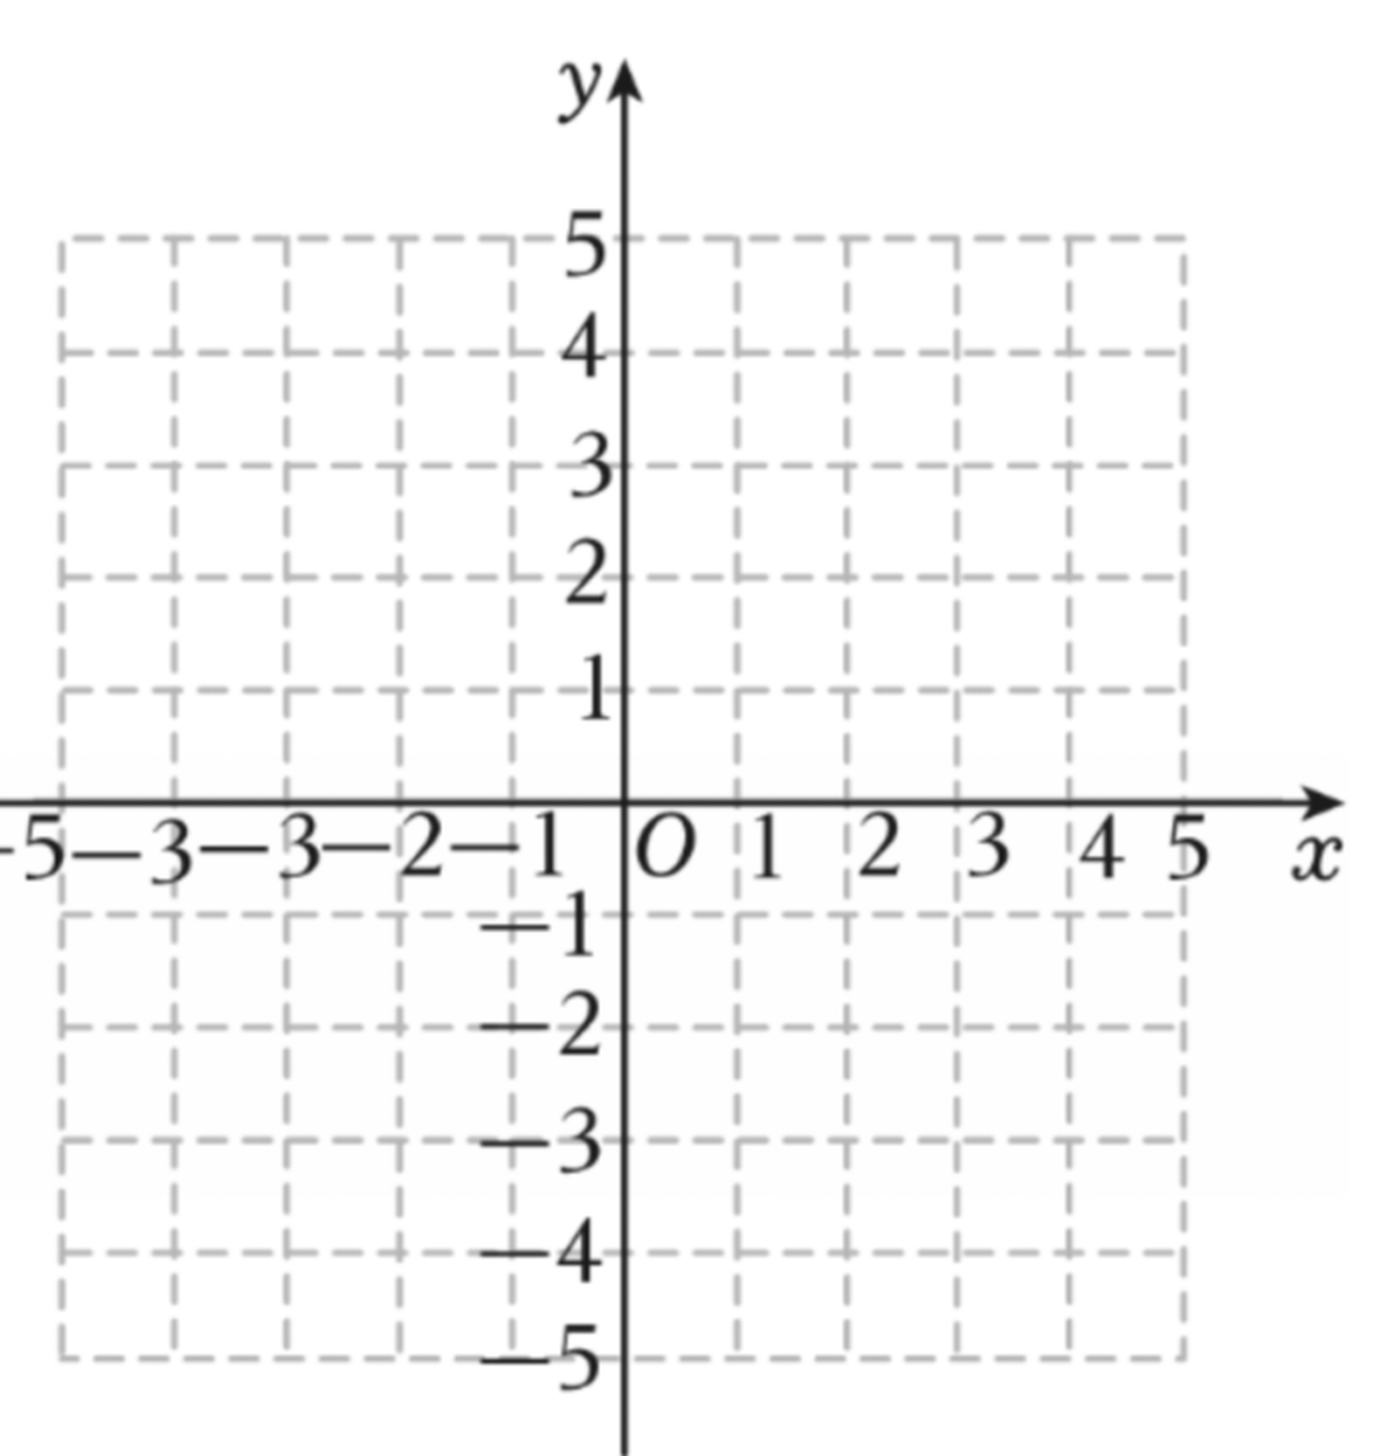
\includegraphics[width=0.52\textwidth]{figures/gao142_q21_grid.png}
\end{center}

\ifanswer
\solbegin
\step{(1) 由题意幂函数 $f(x)=(m^2-3m+3)x^m$，}
\step{故 $m^2-3m+3=1$，解得 $m=1$ 或 $m=2$，}
\step{又 $f(x)$ 图象关于 $y$ 轴对称，即 $f(x)$ 是偶函数，}
\step{当 $m=1$ 时，$f(x)=x$ 是奇函数，不满足条件，舍去；}
\step{当 $m=2$ 时，$f(x)=x^2$ 是偶函数，满足条件，故 $m=2$；}
\step{(2) 由 (1) 得，$\lvert f(x)-1\rvert=\lvert x^2-1\rvert$，}
\step{先画 $y=x^2-1$，开口向上的抛物线，顶点 $(0,-1)$，零点 $x=\pm1$，}
\step{再将 $x$ 轴下方的部分沿 $x$ 轴翻折到上方即为 $y=\lvert x^2-1\rvert$ 的图象，}
\step{图象如图所示.}
\par{\leftskip=0pt
\begin{center}
% 抛物线图象取原卷 09 页截图去粉色水印、去色、LANCZOS 放大；解析所附配图，仅答案版出
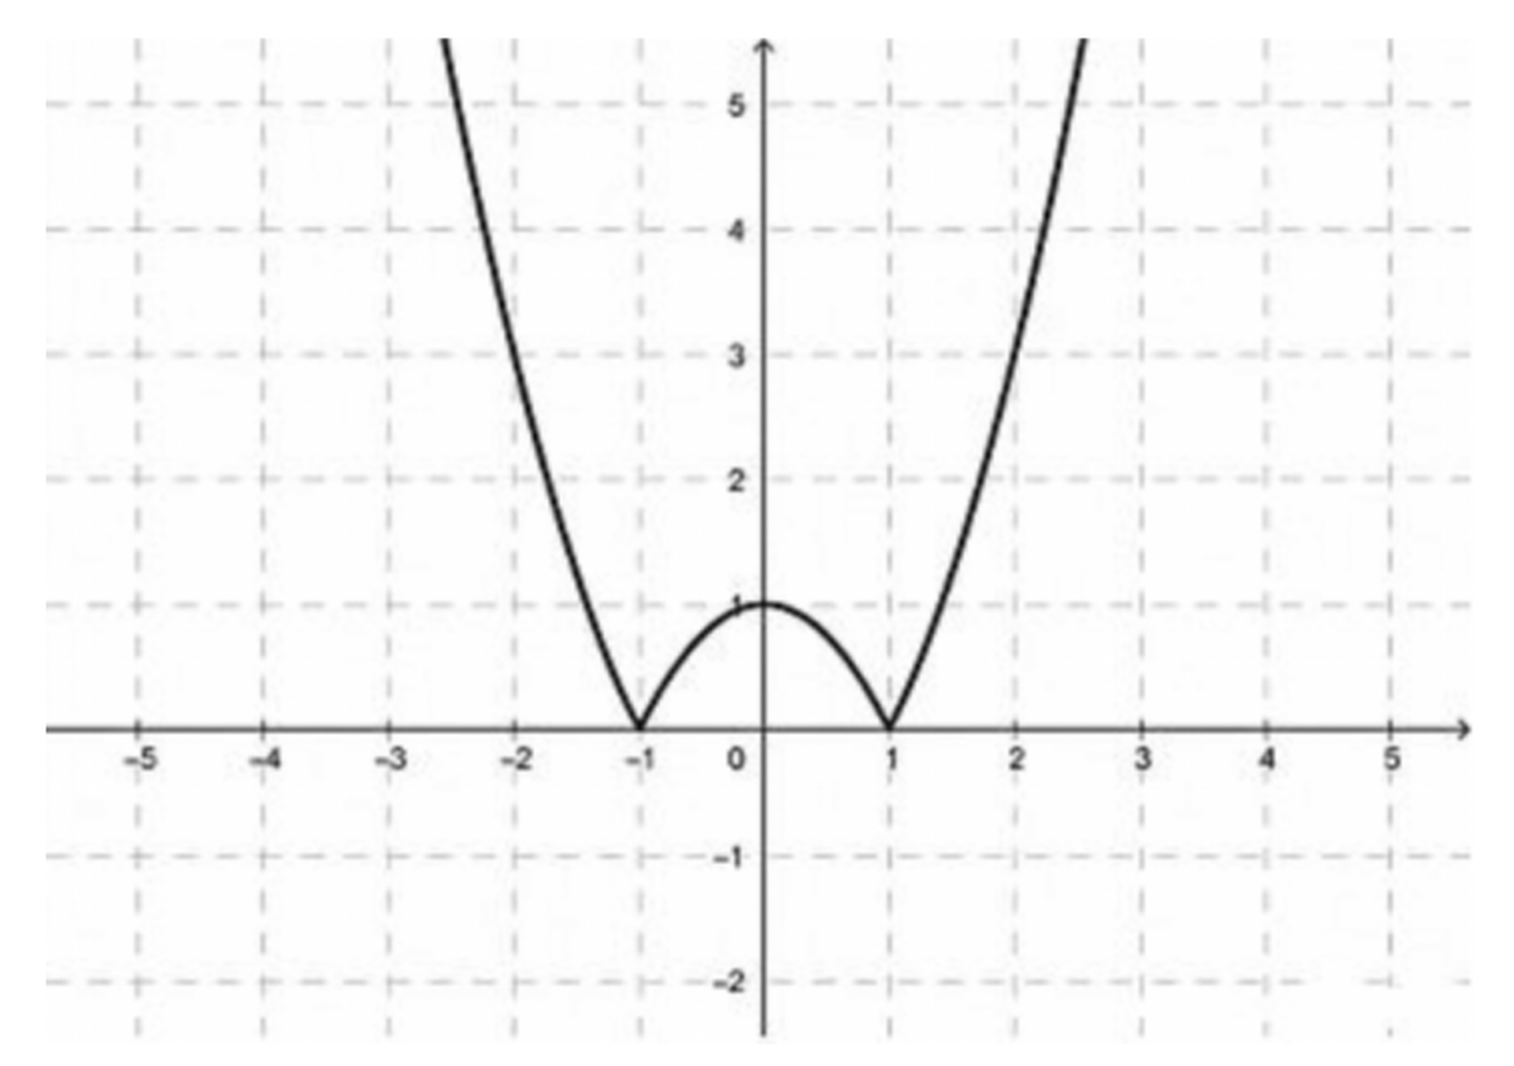
\includegraphics[width=0.55\textwidth]{figures/gao142_q21_para.png}
\end{center}}
\step{(3) 由题意得，$y_1=(2a)^2$，$y_2=(3-a)^2$，}
\step{$y_1<y_2$，即有 $(2a)^2<(3-a)^2$，化简整理得 $(a+3)(a-1)<0$，}
\step{解得实数 $a$ 的取值范围为 $(-3,1)$.}
\solend
\fi

\end{enumerate}

\end{document}
"
%
% ① 原始材料：微信公众号"魔都数学加油站"文章，连载"27学年高一142"，原文标题
% "27学年高一142——2026-2027年上海市群峰高级中学高一上期中"；
% 原文链接：https://mp.weixin.qq.com/s/cc7wnuP4Pk3OjNDV6ihB9A。
% 正文为 9 张 PNG 页（01、02、04、06、07、08、09 为 2560x3620；03、05 为 4762x6735，
% 同一篇各页分辨率不同，逐页按各自分辨率裁图核对），题目下印有【答案】或【解析】，为讲评版。
% 题目、解析均据原图转录；卷面粉红色水印"魔都数学加油站"及公众号页脚未录入。
% 全卷 4 幅插图：第 15 题四幅坐标函数图像选项（04 页，2x2 合并为一张）、
% 第 20 题矩形围栏示意图（07 页）、第 21 题 (2) 空白坐标网格（08 页）、
% 第 21 题抛物线图象（09 页，解析所附图）；均取原卷截图去粉色水印、LANCZOS 放大。
% 题目配图三版都出、解析配图仅答案版出。
%
% 卷首标题：原卷印作"2026-2027 年群峰高级中学高一上期中"（公众号标题中的"上海市"
% 卷面标题行没有，本稿照卷面），年份区间按全稿惯例排 en dash；原卷未印副标题，
% 本卷为期中卷、跨集合与常用逻辑用语／不等式／函数三章，按题目内容补出
% "集合与常用逻辑用语、不等式、函数"（头注说明，与同期中卷口径相同）。
%
% 题号体例：本卷共 19 题——一、填空题 3—12（10 题）、二、选择题 13—16（4 题）、
% 三、解答题 17—21（5 题）。三节分别 \setcounter{enumi}{2}／{12}／{16}。
% 原卷从第 3 题起、无第 1、2 题，本稿保留原题号。
%
% ② 与原卷的排版差异：
%   ① 原文从第 3 题起，本稿保留原题号；原卷未印副标题，本稿按"知识模块"口径补出；
%   ② 逐题答案口径：Q14 原卷把答案 D 印在题干括号内、且题目下无【解析】，本稿括号
%      留空 \mbox{（\quad）}、另提 \ans{D}；Q13／Q15／Q16 答案在【解析】末句"故选 …"
%      （分别为 C／C／A），题干括号留空、不另提 \ans{}；其余各题（Q3—Q12、
%      Q17—Q21）题目下印【解析】、答案融在解析中，不另提 \ans{}；全卷仅 Q14 一处 \ans{}；
%      答案版【答案】/【解析】标记数 = 19（1 个 \ans + 18 个 \solbegin）= 全卷题数；
%   ③ 原卷填空横线按全稿惯例排 \blankline[4.4em]；选择题括号排 \mbox{（\quad）}、
%      每个选项段前按惯例加 \keepwithprev（Q15 四幅图那一枚放在 \begin{center} 之前）；
%      解答题不留作答区、不加 \anspace（原卷为讲评版，与 129／131／132／133／136／140 同）；
%   ④ 原卷数集斜体 $R$（Q5、Q7、Q19、Q21 解析等）按全稿惯例统一改 \R；空集记号
%      \varnothing；绝对值排 \lvert…\rvert，集合描述竖线排 \mid；不等号按全稿惯例
%      排 \leqslant／\geqslant；
%   ⑤ 4 幅插图：Q15 四幅坐标函数图象选项合并裁为一张 \includegraphics（题前
%      \needvspace{9cm}）；Q15 是"二、选择题"节内带大图块的第 3 题（Q13、Q14 在前
%      且无图），另在 \bigsec{二、选择题} 之前加 \needvspace{11cm} 连节标题一起量
%      ——守卫必须放在 \bigsec 之前，放标题之后会让"二、选择题"孤立在页末
%      （B 类，照 高一26／40／59／136／140 成例）；Q20 围栏图与 Q21 网格图置于题干
%      之后（三版都出），Q21 抛物线图置于答案版解析 (2) 与 (3) 之间（仅答案版出）；
%   ⑥ 子题标号按原卷排半角 (1)(2)(3)（与 140／141 同期中卷口径相同）；括注全角／
%      半角逐处照录：Q3"（用含有 m 的代数式表示）"、Q6"（舍）"、Q10"（万元）"、
%      Q18"（请务必书写必要的计算步骤）"、Q20"（墙足够长）"印全角；Q15
%      "$y=a^x(a>0 且 a\neq1)$"、Q10"$y=x^a(a 为常数)$"、Q20"$t=\sqrt{xy}(t>0)$"
%      等数学式内括注印半角；数学式内 CJK 用 \text{…}（否则 FONTCHK 报缺字）；
%   ⑦ 数学式内半角逗号照录（如 Q6"$ax-1=0,a\in\R$"、Q9"$b=2+\sqrt2,a=\sqrt2+1$"、
%      Q16 区间 "$[-1,3]$"、Q21"$y_1<y_2$，即 $(2a)^2<(3-a)^2$" 等）；原卷行末
%      西文句点照录（Q7"(-3,5)."、Q10"125（万元）."、Q19 题干句点、Q20 题干
%      "矩形菜园."与"宽为 y 米."、Q21 题干"对称." 等）；行中全角逗号、分号照录；
%   ⑧ 题干中的中文弯引号：本卷题干与解析通篇未出现中文弯引号，故无此项；
%      圈数字 ①②③ 亦未出现（子题用 (1)(2)(3)）；
%   ⑨ 原卷"图像／图象"两种写法混用，逐处放大核对并照录：Q4 题干与解析作"图象"、
%      Q7 解析作"图象"、Q8 题干作"图像"而解析作"图象"、Q15 题干与解析通篇作
%      "图像"、Q21 题干与解析通篇作"图象"；
%   ⑩ 原卷无红色加粗标签（【解析】均黑色印刷；逐页扫描深红像素为 0），故本卷未用
%      \stepm；黑色常规分步标签（"A 中""C 中""D 中""(1)(2)(3)" 等）按普通 \step
%      行内文字照录；
%   ⑪ 跨页续印按题合并，明细见 ⑥。
%
% ③ 行数复核：一条 \step = 原卷解析的一个印刷行，cases 块作一个印刷行计。逐题数 \step
%   条数，合计 98 条（Q3：1；Q4：2；Q5：3；Q6：4；Q7：5；Q8：2；Q9：4；Q10：3；
%   Q11：4；Q12：3；Q13：5；Q14：0；Q15：10；Q16：4；Q17：10；Q18：3；
%   Q19：10；Q20：13；Q21：12），与原卷印刷行逐题相等。Q14 只把答案印在题干括号、
%   无【解析】，提 \ans{D}、不计入 \step 账；答案版标记数 = 19（1 个 \ans + 18 个
%   \solbegin）= 全卷题数。
%
% ④ 判别式字形：全卷判别式共 3 处——第 7 题【解析】"即判别式△<0"、
%   "即△=(a-1)^2-4×1×4<0" 两处原卷印扁等边三角 $\triangle$，
%   第 11 题【解析】cases 块"△=4a^2-4(a+6)≥0" 一处原卷印等腰偏高的高三角 $\Delta$；
%   逐处放大核对，两形不同、全卷混用，本稿逐处照录不统一（参照 高一141 头注④口径）。
%   子集符号：全卷共 3 处——第 6 题题干"若 B⊆A"、第 6 题【解析】"因为 B⊆A"、
%   第 17 题【解析】(2)"所以 A⊆B"，逐处放大核对，原卷三处均印带下划线的
%   $\subseteq$（不是单线 $\subset$），本稿一律照录 \subseteq；全卷未出现 \subset。
%
% ⑤ 原卷存疑照录（均照录未改，正文对应处另有 % 注）：
%   第 14 题题干括号内原卷印答案 D（非留空），且题目下无【解析】，按"答案印括号且
%      无解析"口径括号留空、另提 \ans{D}；
%   第 15 题【解析】"C 中，由指数函数 … 图像递减得 a>1" 中"递减"与"a>1"
%      自相矛盾（递减应得 0<a<1，疑为"递增"之误），照录；
%   第 16 题选项 B 作 $(-\infty,3]\cup[3,+\infty)$，两端区间并起即全体实数、
%      与正确答案 $[-1,3]$ 不成干扰项（疑为 $(-\infty,-1]\cup[3,+\infty)$ 之误），照录；
%   第 21 题 (2) 空白坐标网格的 x 轴刻度原卷印作"-5 -3 -3 -2 -1 0 1 2 3 4 5"
%      （"-3"重复，疑为"-4"之误），系插图中的印刷内容，取原卷截图照录、不改图。
%
% ⑥ 跨页续印说明：Q7 题干与解析首行在 01 页、解析续至 02 页；Q11 题干与解析
%   4 行在 03 页；Q13 解析前 4 行在 03 页、末句"故选 C."续至 04 页；Q15 题干与
%   四幅图在 04 页、解析前 8 行在 04 页、末 2 行续至 05 页；Q17 解析前 7 行在
%   05 页、后 3 行续至 06 页；Q19 解析前 5 行在 06 页、后 5 行续至 07 页；
%   Q20 解析前 9 行在 07 页、后 4 行续至 08 页；Q21 解析 (1)(2) 9 行在 08 页、
%   抛物线图与 (3) 3 行续至 09 页；本稿按题连排，不丢行。三版切页审计结论见
%   编译自验回报（切页守卫见 ②⑤）。
%
\documentclass[a4paper,11pt]{article}
\usepackage{common}

\begin{document}

\examtitlest[3]{2026--2027 年群峰高级中学高一上期中}{集合与常用逻辑用语、不等式、函数}

\bigsec{一、填空题}

\begin{enumerate}
\setcounter{enumi}{2}

\item 已知 $\log_2 3=m$，则 $\log_3 6=$\blankline[4.4em]（用含有 $m$ 的代数式表示）.

\ifanswer
\solbegin
\step{$\log_3 6=\dfrac{\log_2 6}{\log_2 3}=\dfrac{\log_2 2+\log_2 3}{\log_2 3}=\dfrac{1+m}{m}=\dfrac1m+1$.}
\solend
\fi

\item 若指数函数 $y=a^x$ 的图象经过点 $(3,27)$，则 $a$ 的值为\blankline[4.4em].

\ifanswer
\solbegin
\step{因为指数函数 $y=a^x$ 的图象经过点 $(3,27)$，}
\step{所以 $a^3=27=3^3$，所以 $a=3$.}
\solend
\fi

\item 不等式 $(2x+1)^{\frac13}<(3-x)^{\frac13}$ 的解集为\blankline[4.4em].

\ifanswer
\solbegin
\step{因为幂函数 $f(t)=t^{\frac13}$ 在 $\R$ 上严格增，}
\step{所以原不等式等价于 $2x+1<3-x$，解得 $x<\dfrac23$，}
\step{因此原不等式的解集为 $\left(-\infty,\dfrac23\right)$.}
\solend
\fi

\item 设集合 $A=\{1,-2\}$，$B=\{x\mid ax-1=0,a\in\R\}$，若 $B\subseteq A$，则 $a$ 的值为\blankline[4.4em].% 子集符号原卷印带下划线 $\subseteq$，照录

\ifanswer
\solbegin
\step{因为 $B\subseteq A$，所以 $B=\varnothing$ 或 $\{-2\}$ 或 $\{1\}$ 或 $\{1,-2\}$（舍），}% 子集符号原卷印带下划线 $\subseteq$，照录
\step{若 $B=\varnothing$，则 $a=0$；若 $B=\{1\}$，则 $a=1$；}
\step{若 $B=\{-2\}$，则 $-2a=1$，解得 $a=-\dfrac12$；}
\step{综上，$a=0$ 或 $1$ 或 $-\dfrac12$.}
\solend
\fi

\item 不等式 $x^2+(a-1)x+4>0$ 在 $\R$ 上恒成立，则实数 $a$ 的取值范围是\blankline[4.4em].

\ifanswer
\solbegin
\step{不等式 $x^2+(a-1)x+4>0$，对应的二次函数为 $y=x^2+(a-1)x+4$，}
\step{因此函数图象开口向上，要使不等式对任意实数 $x$ 恒成立，}
\step{需二次函数图象与 $x$ 轴无交点，即判别式 $\triangle<0$，}% 判别式原卷印扁等边三角 $\triangle$，照录
\step{即 $\triangle=(a-1)^2-4\times1\times4<0$，整理得 $a^2-2a-15<0$，}% 判别式原卷印扁等边三角 $\triangle$，照录
\step{解得 $-3<a<5$，故实数 $a$ 的取值范围是 $(-3,5)$.}
\solend
\fi

\item 函数 $f(x)=(5x-3)^a$ 的图像恒过点\blankline[4.4em].% 题干作"图像"、解析作"图象"，原卷混用，逐处照录

\ifanswer
\solbegin
\step{令 $5x-3=1$ 得 $x=\dfrac45$，此时 $f\left(\dfrac45\right)=\left(5\times\dfrac45-3\right)^a=1$，}
\step{所以 $f(x)$ 的图象恒过 $\left(\dfrac45,1\right)$.}
\solend
\fi

\item 若 $a>0$，$b>0$ 且 $\dfrac1a+\dfrac2b=1$，则 $a+b$ 的最小值为\blankline[4.4em].

\ifanswer
\solbegin
\step{因为 $a>0$，$b>0$，$\dfrac1a+\dfrac2b=1$，}
\step{所以 $a+b=(a+b)\left(\dfrac1a+\dfrac2b\right)=1+\dfrac{2a}{b}+\dfrac{b}{a}+2\geqslant3+2\sqrt{\dfrac{2a}{b}\cdot\dfrac{b}{a}}=3+2\sqrt2$，}
\step{当且仅当 $\dfrac{2a}{b}=\dfrac{b}{a}$，即 $b=2+\sqrt2,a=\sqrt2+1$ 时取等号，}
\step{故 $a+b$ 的最小值为 $3+2\sqrt2$.}
\solend
\fi

\item 某药厂研制出一种新型药剂，投放市场后其广告投入 $x$（万元）与药品利润 $y$（万元）存在的关系为 $y=x^a(a\text{ 为常数})$，其中 $x$ 不超过 5 万元. 已知去年投入广告费用为 3 万元时，药品利润为 27 万元，若今年投入广告费用 5 万元，预计今年药品利润为\blankline[4.4em]万元.

\ifanswer
\solbegin
\step{由已知投入广告费用为 3 万元时，药品利润为 27 万元，}
\step{代入 $y=x^a$ 中，即 $3^a=27$，解得 $a=3$，故函数关系式为 $y=x^3$，}
\step{所以当 $x=5$ 时，$y=125$（万元）.}
\solend
\fi

\item 已知方程 $x^2+2ax+a+6=0$ 的两根分别是 $x_1$ 和 $x_2$，且满足 $\dfrac1{x_1}+\dfrac1{x_2}<0$，则实数 $a$ 的取值范围是\blankline[4.4em].

\ifanswer
\solbegin
\step{由于方程 $x^2+2ax+a+6=0$ 的两根分别是 $x_1$ 和 $x_2$，}
\step{则 $\begin{cases}\Delta=4a^2-4(a+6)\geqslant0\\x_1+x_2=-2a\\x_1x_2=a+6\end{cases}$，解得 $a\geqslant3$ 或 $a\leqslant-2$.}% 判别式原卷印等腰偏高的高三角 $\Delta$，照录（与第 7 题扁等边 $\triangle$ 两形混用）
\step{又 $\dfrac1{x_1}+\dfrac1{x_2}<0$，即 $\dfrac{x_1+x_2}{x_1\cdot x_2}<0$，故 $\dfrac{-2a}{a+6}<0$，解得 $a<-6$ 或 $a>0$.}
\step{综上，$a$ 的取值范围是 $(-\infty,-6)\cup[3,+\infty)$.}
\solend
\fi

\item 已知 $b>a>1$，若 $\log_a b-\log_b a=\dfrac32$，$a^b=b^a$，则 $a-b=$\blankline[4.4em].

\ifanswer
\solbegin
\step{因为 $b>a>1$，所以 $\log_a b>1$，}
\step{由 $\log_a b-\log_b a=\log_a b-\dfrac{1}{\log_a b}=\dfrac32$，解得 $\log_a b=2$ 即 $b=a^2$，}
\step{因为 $a^b=b^a=a^{2a}$，所以 $b=2a=a^2$，所以 $a=2$，$b=4$，则 $a-b=-2$.}
\solend
\fi

\end{enumerate}

% 第 15 题四幅图是"二、选择题"节内的大图块；守卫须放在 \bigsec 之前连节标题一起量
\needvspace{11cm}
\bigsec{二、选择题}

\begin{enumerate}
\setcounter{enumi}{12}

\item 若 $a>b$，$c<0$，则下列不等式正确的是\mbox{（\quad）}

\keepwithprev
A. $ab>bc$\qquad B. $a+c<b+c$\qquad C. $ac^2>bc^2$\qquad D. $\dfrac ac>\dfrac bc$

\ifanswer
\solbegin
\step{因为 $a>b$，$c<0$，取 $b=0$，则 $ab=bc=0$，故 $A$ 错误；}
\step{由于 $a>b$，所以 $a+c>b+c$，故 $B$ 错误；}
\step{由 $c<0$ 得 $c^2>0$，所以 $ac^2>bc^2$，故 $C$ 正确；}
\step{由于 $a>b$ 且 $c<0$，所以 $\dfrac ac<\dfrac bc$，故 $D$ 错误.}
\step{故选 $C$.}
\solend
\fi

\item 若 $x>0$，$y>0$，则下列各式中，恒成立的是\mbox{（\quad）}% 原卷题干括号内印答案 D、且题目下无【解析】，本稿括号留空、另提 \ans{D}

\keepwithprev
A. $\lg x+\lg y=\lg(x+y)$\qquad B. $\lg x^2=(\lg x)^2$

C. $\dfrac{\lg x}{\lg y}=\lg(x-y)$\qquad D. $\lg x^{\frac1n}=\dfrac{\lg x}{n}$

\ifanswer
\ans{$D$}
\fi

% 第 15 题四幅坐标函数图象选项是一整块，守卫放在 \item 之前
\needvspace{9cm}
\item 在同一平面直角坐标系中，指数函数 $y=a^x(a>0\text{ 且 }a\neq1)$ 和一次函数 $y=a(x+1)$ 的图像关系可能是\mbox{（\quad）}

\keepwithprev
\begin{center}
% 四幅坐标函数图象选项取原卷 04 页截图去粉色水印、去色，按原卷 2x2 排布合并为一张
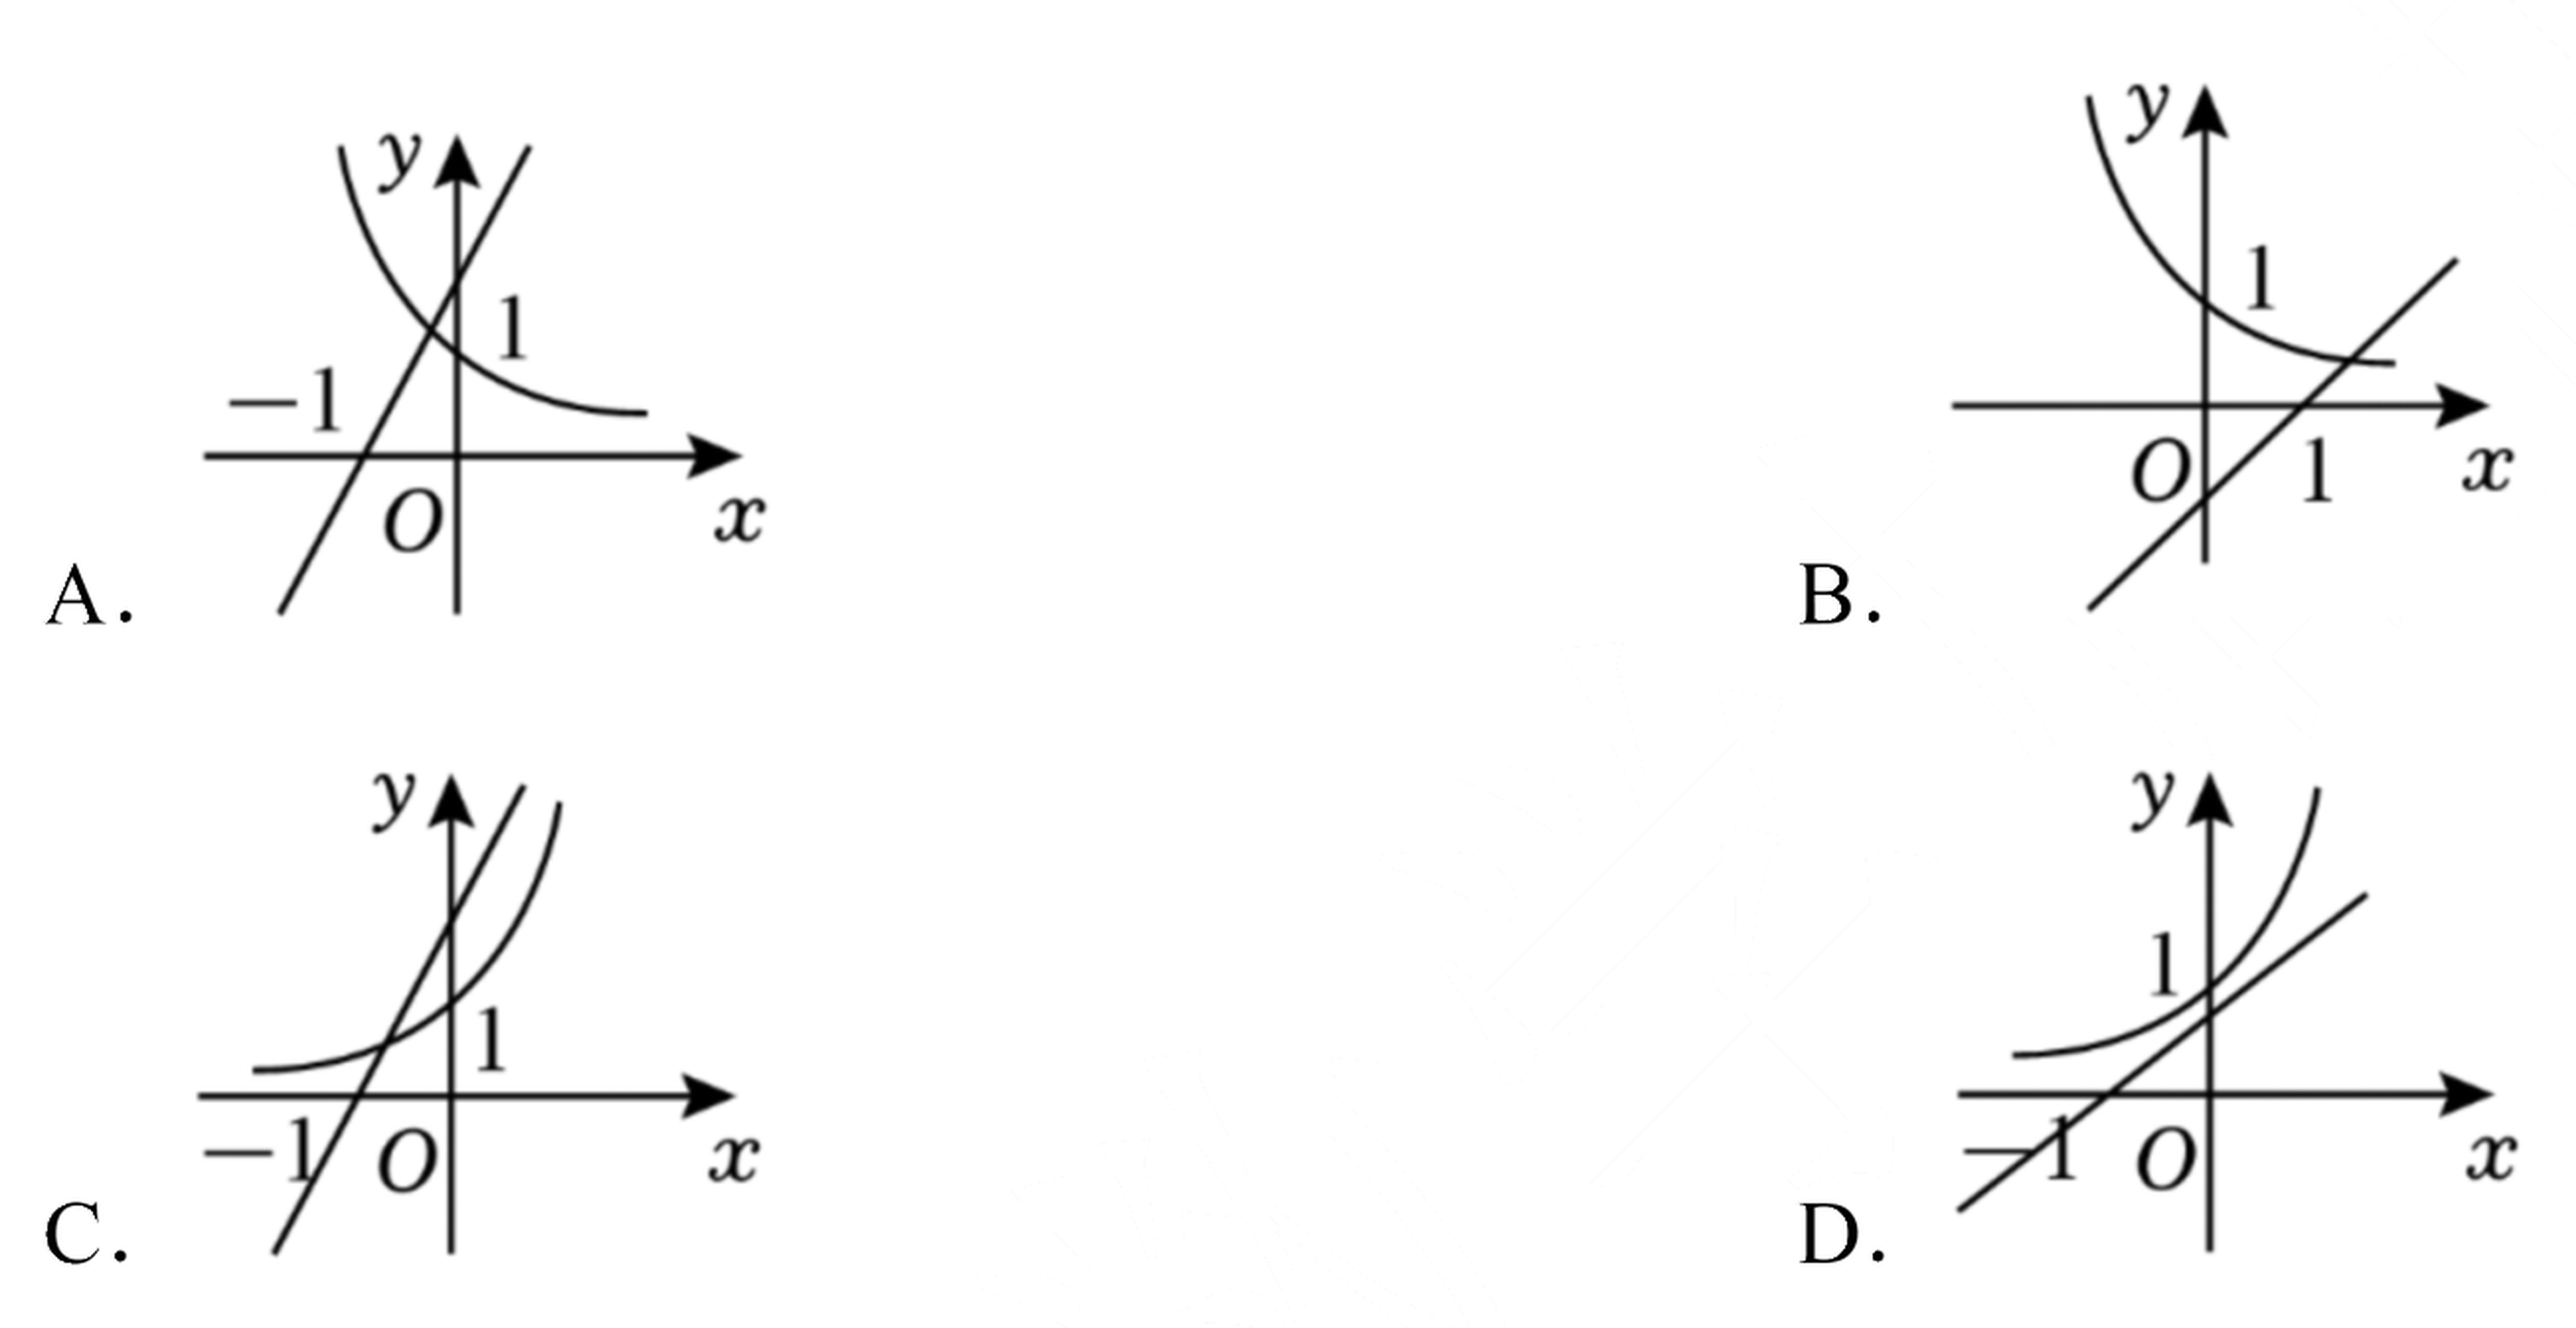
\includegraphics[width=0.80\textwidth]{figures/gao142_q15.png}
\end{center}

\ifanswer
\solbegin
\step{$A$ 中，由指数函数 $y=a^x(a>0\text{ 且 }a\neq1)$ 图像递减得 $0<a<1$，}
\step{而一次函数 $y=a(x+1)$ 的图像与 $y$ 轴交点纵坐标为 $a>1$，二者矛盾，}
\step{所以 $A$ 错；}
\step{由一次函数 $y=a(x+1)$ 的图像与 $x$ 轴交点横坐标为 $-1$，排除 $B$；}
\step{$C$ 中，由指数函数 $y=a^x(a>0\text{ 且 }a\neq1)$ 图像递减得 $a>1$，}% 原卷"递减得 a>1"自相矛盾（递减应得 0<a<1），照录
\step{而一次函数 $y=a(x+1)$ 的图像与 $y$ 轴交点纵坐标为 $a>1$，二者 $a$ 值吻合，}
\step{所以 $C$ 对；}
\step{$D$ 中，由一次函数 $y=a(x+1)$ 的图像得 $a=1$，与 $a>0$ 且 $a\neq1$ 矛盾，}
\step{所以 $D$ 错.}
\step{故选 $C$.}
\solend
\fi

\item 不等式 $\lvert x+1\rvert+\lvert 2-x\rvert\geqslant a^2-2a$ 恒成立，则 $a$ 的取值范围是\mbox{（\quad）}

\keepwithprev
A. $[-1,3]$\qquad B. $(-\infty,3]\cup[3,+\infty)$\qquad C. $(-\infty,3)$\qquad D. $(3,+\infty)$

\ifanswer
\solbegin
\step{因为 $\lvert x+1\rvert+\lvert 2-x\rvert\geqslant\lvert(x+1)+(2-x)\rvert=3$，}
\step{所以 $\lvert x+1\rvert+\lvert 2-x\rvert$ 的最小值为 3，}
\step{因为 $\lvert x+1\rvert+\lvert 2-x\rvert\geqslant a^2-2a$ 恒成立，所以只需 $a^2-2a\leqslant3$，所以 $-1\leqslant a\leqslant3$，}
\step{所以 $a$ 的取值范围为 $[-1,3]$. 故选 $A$.}
\solend
\fi

\end{enumerate}

\bigsec{三、解答题}

\begin{enumerate}
\setcounter{enumi}{16}

\item 已知集合 $A=\left\{x\mid\dfrac{x-3}{x-1}\leqslant0\right\}$，$B=\{x\mid\lvert x-1\rvert<a\}$.

(1) 若 $a=1$，求 $A\cap B$；

(2) 若 $x\in A$ 是 $x\in B$ 的充分条件，求 $a$ 的取值范围.

\ifanswer
\solbegin
\step{(1) 不等式 $\dfrac{x-3}{x-1}\leqslant0$，等价于 $(x-3)(x-1)\leqslant0$ 且 $x-1\neq0$，解得 $1<x\leqslant3$，}
\step{所以 $A=\{x\mid 1<x\leqslant3\}$，}
\step{当 $a=1$ 时，不等式 $\lvert x-1\rvert<a$ 可化为 $\lvert x-1\rvert<1$，所以 $-1<x-1<1$，}
\step{故 $0<x<2$，所以 $B=\{x\mid 0<x<2\}$，}
\step{所以 $A\cap B=\{x\mid 1<x<2\}$；}
\step{(2) 因为 $x\in A$ 是 $x\in B$ 的充分条件，所以 $A\subseteq B$，}% 子集符号原卷印带下划线 $\subseteq$，照录
\step{因为 $A=\{x\mid 1<x\leqslant3\}\neq\varnothing$，所以 $B\neq\varnothing$，故 $a>0$，}
\step{由不等式 $\lvert x-1\rvert<a$，解得 $1-a<x<1+a$，}
\step{所以 $B=\{x\mid 1-a<x<1+a\}$，所以 $\begin{cases}1-a\leqslant1\\1+a>3\end{cases}$，解得 $a>2$，}
\step{所以 $a$ 的取值范围为 $(2,+\infty)$.}
\solend
\fi

\item 计算下列式子的值（请务必书写必要的计算步骤）

(1) $27^{\frac13}+\left(\dfrac76\right)^0+\sqrt{(3-\pi)^2}$；

(2) $\lg25+\lg4+7^{\log_7 2}-\log_2 3\times\log_3 4+\log_3 9$.

\ifanswer
\solbegin
\step{(1) $27^{\frac13}+\left(\dfrac76\right)^0+\sqrt{(3-\pi)^2}=3^{3\times\frac13}+1+\lvert 3-\pi\rvert=3+1+\pi-3=\pi+1$；}
\step{(2) 原式 $=\lg(25\times4)+2-\dfrac{\lg3}{\lg2}\times\dfrac{\lg4}{\lg3}+2=\lg100+2-\dfrac{2\lg2}{\lg2}+2$}
\step{$=2+2-2+2=4$.}
\solend
\fi

\item 已知关于 $x$ 的不等式 $mx^2-(3m^2-m+2)x+6m-2\geqslant0$.

(1) 当 $m=2$ 时，求关于 $x$ 的不等式的解集；

(2) 当 $m>0$ 时，求关于 $x$ 的不等式的解集.

\ifanswer
\solbegin
\step{(1) $m=2$ 时，不等式为 $x^2-6x+5\geqslant0$，即 $(x-1)(x-5)\geqslant0$，}
\step{解得 $x\leqslant1$ 或 $x\geqslant5$，所以不等式的解集是 $\{x\mid x\leqslant1$ 或 $x\geqslant5\}$.}
\step{(2) $m>0$ 时，不等式可化为 $(mx-2)[x-(3m-1)]\geqslant0$，}
\step{即 $\left(x-\dfrac2m\right)[x-(3m-1)]\geqslant0$，}
\step{若 $m=1$，则不等式为 $(x-2)^2\geqslant0$，解得 $x\in\R$；}
\step{若 $0<m<1$，则 $\dfrac2m>3m-1$，解不等式得 $x\geqslant\dfrac2m$ 或 $x\leqslant3m-1$；}
\step{若 $m>1$，则 $\dfrac2m<3m-1$，解不等式得 $x\geqslant3m-1$ 或 $x\leqslant\dfrac2m$；}
\step{综上，$0<m<1$ 时，不等式的解集是 $\{x\mid x\leqslant3m-1$ 或 $x\geqslant\dfrac2m\}$；}
\step{$m=1$ 时，不等式的解集为 $\R$；}
\step{$m>1$ 时，不等式的解集是 $\{x\mid x\leqslant\dfrac2m$ 或 $x\geqslant3m-1\}$.}
\solend
\fi

\item 如图，某人计划用篱笆围成一个一边靠墙（墙足够长）的矩形菜园. 设菜园的长为 $x$ 米，宽为 $y$ 米.

\begin{center}
% 矩形围栏示意图取原卷 07 页截图去粉色水印、去色、LANCZOS 放大；题目配图，三版都出
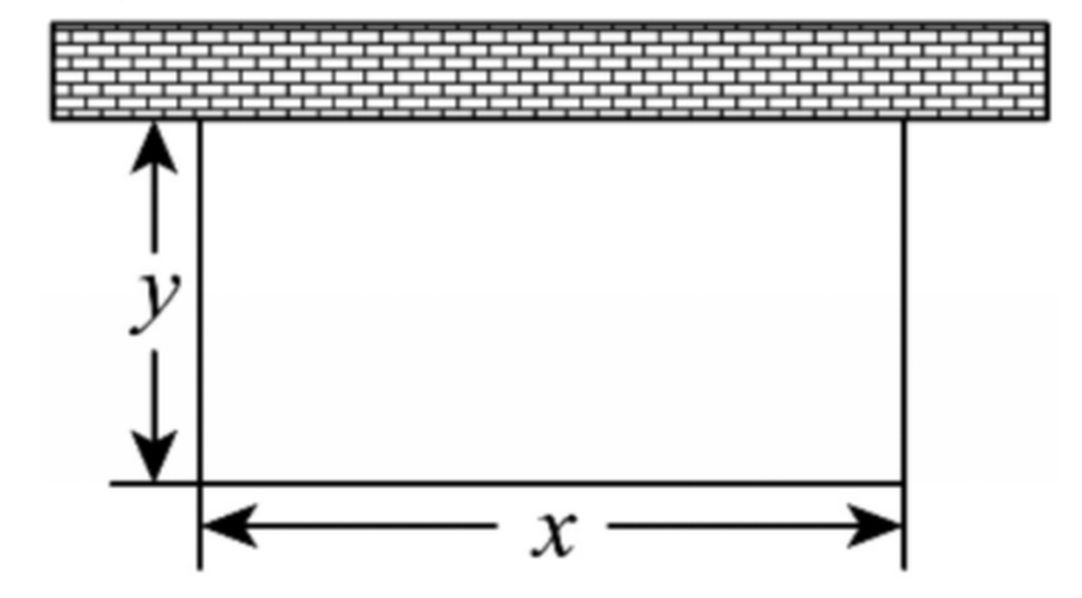
\includegraphics[width=0.42\textwidth]{figures/gao142_q20.png}
\end{center}

(1) 若菜园面积为 72 平方米，则 $x$、$y$ 为何值时，所用篱笆总长最小？

(2) 若 $x$、$y$ 满足 $x+y-xy+63=0$，则菜园面积最小为多少平方米？

\ifanswer
\solbegin
\step{(1) 由题意得，菜园的面积 $S=xy=72$，且 $x>0$，$y>0$，}
\step{所用篱笆总长 $L=x+2y$，}
\step{由基本不等式得 $x+2y\geqslant2\sqrt{x\cdot2y}=2\sqrt{2xy}=2\sqrt{2\times72}=24$，}
\step{当且仅当 $x=2y$ 时取等号，}
\step{联立 $\begin{cases}xy=72\\x=2y\end{cases}$，解得 $\begin{cases}x=12\\y=6\end{cases}$，}
\step{所以当 $x=12$，$y=6$ 时，所用篱笆总长最小；}
\step{(2) 由题意得 $x>0$，$y>0$，且满足 $x+y-xy+63=0$，即 $x+y=xy-63$，}
\step{由基本不等式得 $x+y\geqslant2\sqrt{xy}$，当且仅当 $x=y$ 时取等号，}
\step{所以 $xy-63\geqslant2\sqrt{xy}$. 令 $t=\sqrt{xy}(t>0)$，则 $xy=t^2$，}
\step{上述不等式可化为 $t^2-2t-63\geqslant0$，即 $(t-9)(t+7)\geqslant0$，}
\step{因为 $t>0$，所以 $t+7>0$，故 $t-9\geqslant0$，解得 $t\geqslant9$，所以 $\sqrt{xy}\geqslant9$，}
\step{即 $xy\geqslant81$，当且仅当 $x=y=9$ 时取等号，此时满足 $9+9-81+63=0$，}
\step{所以菜园面积最小为 81 平方米.}
\solend
\fi

\item 已知幂函数 $f(x)=(m^2-3m+3)x^m$ 的图象关于 $y$ 轴对称.

(1) 求实数 $m$ 的值；

(2) 在平面直角坐标系中作出函数 $y=\lvert f(x)-1\rvert$ 的图象；

(3) 已知点 $A(2a,y_1)$ 与点 $B(3-a,y_2)$ 都在幂函数 $y=x^2$ 的图象上. 若 $y_1<y_2$，求实数 $a$ 的取值范围.

\begin{center}
% 空白坐标网格取原卷 08 页截图去粉色水印、去色、LANCZOS 放大；题目配图，三版都出
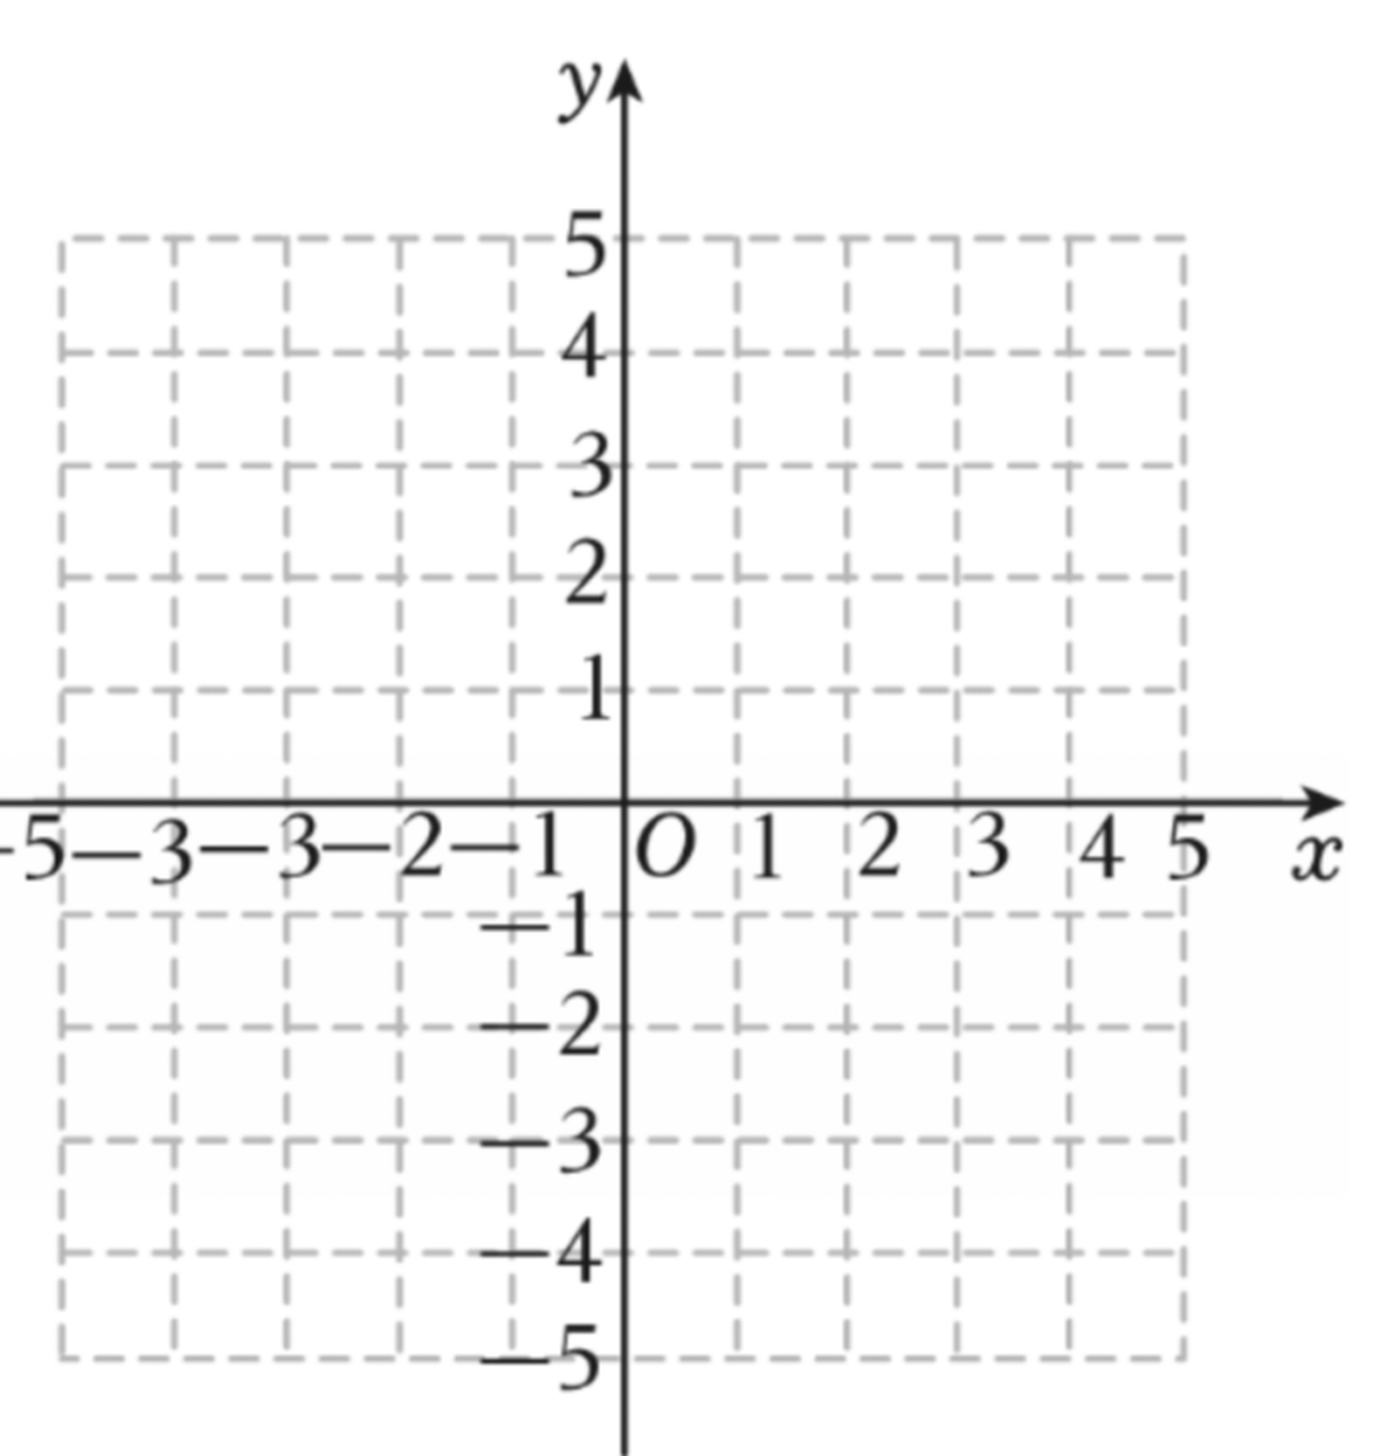
\includegraphics[width=0.52\textwidth]{figures/gao142_q21_grid.png}
\end{center}

\ifanswer
\solbegin
\step{(1) 由题意幂函数 $f(x)=(m^2-3m+3)x^m$，}
\step{故 $m^2-3m+3=1$，解得 $m=1$ 或 $m=2$，}
\step{又 $f(x)$ 图象关于 $y$ 轴对称，即 $f(x)$ 是偶函数，}
\step{当 $m=1$ 时，$f(x)=x$ 是奇函数，不满足条件，舍去；}
\step{当 $m=2$ 时，$f(x)=x^2$ 是偶函数，满足条件，故 $m=2$；}
\step{(2) 由 (1) 得，$\lvert f(x)-1\rvert=\lvert x^2-1\rvert$，}
\step{先画 $y=x^2-1$，开口向上的抛物线，顶点 $(0,-1)$，零点 $x=\pm1$，}
\step{再将 $x$ 轴下方的部分沿 $x$ 轴翻折到上方即为 $y=\lvert x^2-1\rvert$ 的图象，}
\step{图象如图所示.}
\par{\leftskip=0pt
\begin{center}
% 抛物线图象取原卷 09 页截图去粉色水印、去色、LANCZOS 放大；解析所附配图，仅答案版出
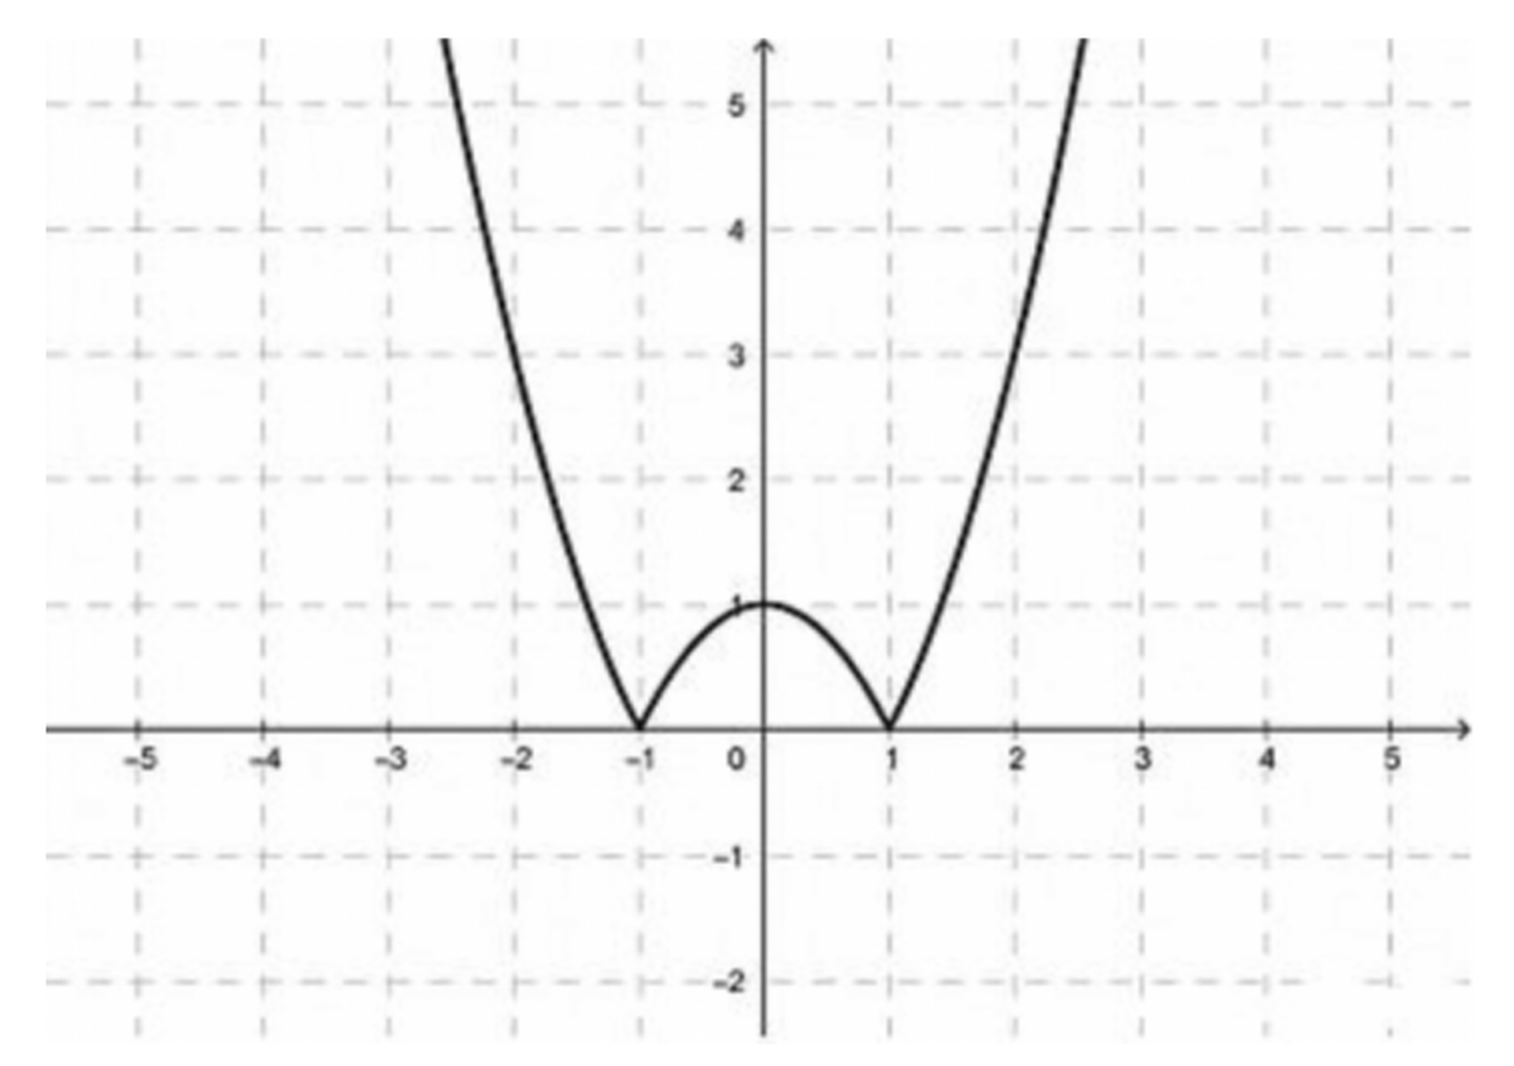
\includegraphics[width=0.55\textwidth]{figures/gao142_q21_para.png}
\end{center}}
\step{(3) 由题意得，$y_1=(2a)^2$，$y_2=(3-a)^2$，}
\step{$y_1<y_2$，即有 $(2a)^2<(3-a)^2$，化简整理得 $(a+3)(a-1)<0$，}
\step{解得实数 $a$ 的取值范围为 $(-3,1)$.}
\solend
\fi

\end{enumerate}

\end{document}
"
% 紧凑版：xelatex "\def\iscompact{1}% 高一142_群峰高级中学_期中.tex
%   —— 高一上数学"2026-2027 年群峰高级中学高一上期中"（试卷版/答案版）
% 试卷版：xelatex 高一142_群峰高级中学_期中.tex
% 答案版：xelatex "\def\isanswer{1}% 高一142_群峰高级中学_期中.tex
%   —— 高一上数学"2026-2027 年群峰高级中学高一上期中"（试卷版/答案版）
% 试卷版：xelatex 高一142_群峰高级中学_期中.tex
% 答案版：xelatex "\def\isanswer{1}\input{高一142_群峰高级中学_期中.tex}"
% 紧凑版：xelatex "\def\iscompact{1}\input{高一142_群峰高级中学_期中.tex}"
%
% ① 原始材料：微信公众号"魔都数学加油站"文章，连载"27学年高一142"，原文标题
% "27学年高一142——2026-2027年上海市群峰高级中学高一上期中"；
% 原文链接：https://mp.weixin.qq.com/s/cc7wnuP4Pk3OjNDV6ihB9A。
% 正文为 9 张 PNG 页（01、02、04、06、07、08、09 为 2560x3620；03、05 为 4762x6735，
% 同一篇各页分辨率不同，逐页按各自分辨率裁图核对），题目下印有【答案】或【解析】，为讲评版。
% 题目、解析均据原图转录；卷面粉红色水印"魔都数学加油站"及公众号页脚未录入。
% 全卷 4 幅插图：第 15 题四幅坐标函数图像选项（04 页，2x2 合并为一张）、
% 第 20 题矩形围栏示意图（07 页）、第 21 题 (2) 空白坐标网格（08 页）、
% 第 21 题抛物线图象（09 页，解析所附图）；均取原卷截图去粉色水印、LANCZOS 放大。
% 题目配图三版都出、解析配图仅答案版出。
%
% 卷首标题：原卷印作"2026-2027 年群峰高级中学高一上期中"（公众号标题中的"上海市"
% 卷面标题行没有，本稿照卷面），年份区间按全稿惯例排 en dash；原卷未印副标题，
% 本卷为期中卷、跨集合与常用逻辑用语／不等式／函数三章，按题目内容补出
% "集合与常用逻辑用语、不等式、函数"（头注说明，与同期中卷口径相同）。
%
% 题号体例：本卷共 19 题——一、填空题 3—12（10 题）、二、选择题 13—16（4 题）、
% 三、解答题 17—21（5 题）。三节分别 \setcounter{enumi}{2}／{12}／{16}。
% 原卷从第 3 题起、无第 1、2 题，本稿保留原题号。
%
% ② 与原卷的排版差异：
%   ① 原文从第 3 题起，本稿保留原题号；原卷未印副标题，本稿按"知识模块"口径补出；
%   ② 逐题答案口径：Q14 原卷把答案 D 印在题干括号内、且题目下无【解析】，本稿括号
%      留空 \mbox{（\quad）}、另提 \ans{D}；Q13／Q15／Q16 答案在【解析】末句"故选 …"
%      （分别为 C／C／A），题干括号留空、不另提 \ans{}；其余各题（Q3—Q12、
%      Q17—Q21）题目下印【解析】、答案融在解析中，不另提 \ans{}；全卷仅 Q14 一处 \ans{}；
%      答案版【答案】/【解析】标记数 = 19（1 个 \ans + 18 个 \solbegin）= 全卷题数；
%   ③ 原卷填空横线按全稿惯例排 \blankline[4.4em]；选择题括号排 \mbox{（\quad）}、
%      每个选项段前按惯例加 \keepwithprev（Q15 四幅图那一枚放在 \begin{center} 之前）；
%      解答题不留作答区、不加 \anspace（原卷为讲评版，与 129／131／132／133／136／140 同）；
%   ④ 原卷数集斜体 $R$（Q5、Q7、Q19、Q21 解析等）按全稿惯例统一改 \R；空集记号
%      \varnothing；绝对值排 \lvert…\rvert，集合描述竖线排 \mid；不等号按全稿惯例
%      排 \leqslant／\geqslant；
%   ⑤ 4 幅插图：Q15 四幅坐标函数图象选项合并裁为一张 \includegraphics（题前
%      \needvspace{9cm}）；Q15 是"二、选择题"节内带大图块的第 3 题（Q13、Q14 在前
%      且无图），另在 \bigsec{二、选择题} 之前加 \needvspace{11cm} 连节标题一起量
%      ——守卫必须放在 \bigsec 之前，放标题之后会让"二、选择题"孤立在页末
%      （B 类，照 高一26／40／59／136／140 成例）；Q20 围栏图与 Q21 网格图置于题干
%      之后（三版都出），Q21 抛物线图置于答案版解析 (2) 与 (3) 之间（仅答案版出）；
%   ⑥ 子题标号按原卷排半角 (1)(2)(3)（与 140／141 同期中卷口径相同）；括注全角／
%      半角逐处照录：Q3"（用含有 m 的代数式表示）"、Q6"（舍）"、Q10"（万元）"、
%      Q18"（请务必书写必要的计算步骤）"、Q20"（墙足够长）"印全角；Q15
%      "$y=a^x(a>0 且 a\neq1)$"、Q10"$y=x^a(a 为常数)$"、Q20"$t=\sqrt{xy}(t>0)$"
%      等数学式内括注印半角；数学式内 CJK 用 \text{…}（否则 FONTCHK 报缺字）；
%   ⑦ 数学式内半角逗号照录（如 Q6"$ax-1=0,a\in\R$"、Q9"$b=2+\sqrt2,a=\sqrt2+1$"、
%      Q16 区间 "$[-1,3]$"、Q21"$y_1<y_2$，即 $(2a)^2<(3-a)^2$" 等）；原卷行末
%      西文句点照录（Q7"(-3,5)."、Q10"125（万元）."、Q19 题干句点、Q20 题干
%      "矩形菜园."与"宽为 y 米."、Q21 题干"对称." 等）；行中全角逗号、分号照录；
%   ⑧ 题干中的中文弯引号：本卷题干与解析通篇未出现中文弯引号，故无此项；
%      圈数字 ①②③ 亦未出现（子题用 (1)(2)(3)）；
%   ⑨ 原卷"图像／图象"两种写法混用，逐处放大核对并照录：Q4 题干与解析作"图象"、
%      Q7 解析作"图象"、Q8 题干作"图像"而解析作"图象"、Q15 题干与解析通篇作
%      "图像"、Q21 题干与解析通篇作"图象"；
%   ⑩ 原卷无红色加粗标签（【解析】均黑色印刷；逐页扫描深红像素为 0），故本卷未用
%      \stepm；黑色常规分步标签（"A 中""C 中""D 中""(1)(2)(3)" 等）按普通 \step
%      行内文字照录；
%   ⑪ 跨页续印按题合并，明细见 ⑥。
%
% ③ 行数复核：一条 \step = 原卷解析的一个印刷行，cases 块作一个印刷行计。逐题数 \step
%   条数，合计 98 条（Q3：1；Q4：2；Q5：3；Q6：4；Q7：5；Q8：2；Q9：4；Q10：3；
%   Q11：4；Q12：3；Q13：5；Q14：0；Q15：10；Q16：4；Q17：10；Q18：3；
%   Q19：10；Q20：13；Q21：12），与原卷印刷行逐题相等。Q14 只把答案印在题干括号、
%   无【解析】，提 \ans{D}、不计入 \step 账；答案版标记数 = 19（1 个 \ans + 18 个
%   \solbegin）= 全卷题数。
%
% ④ 判别式字形：全卷判别式共 3 处——第 7 题【解析】"即判别式△<0"、
%   "即△=(a-1)^2-4×1×4<0" 两处原卷印扁等边三角 $\triangle$，
%   第 11 题【解析】cases 块"△=4a^2-4(a+6)≥0" 一处原卷印等腰偏高的高三角 $\Delta$；
%   逐处放大核对，两形不同、全卷混用，本稿逐处照录不统一（参照 高一141 头注④口径）。
%   子集符号：全卷共 3 处——第 6 题题干"若 B⊆A"、第 6 题【解析】"因为 B⊆A"、
%   第 17 题【解析】(2)"所以 A⊆B"，逐处放大核对，原卷三处均印带下划线的
%   $\subseteq$（不是单线 $\subset$），本稿一律照录 \subseteq；全卷未出现 \subset。
%
% ⑤ 原卷存疑照录（均照录未改，正文对应处另有 % 注）：
%   第 14 题题干括号内原卷印答案 D（非留空），且题目下无【解析】，按"答案印括号且
%      无解析"口径括号留空、另提 \ans{D}；
%   第 15 题【解析】"C 中，由指数函数 … 图像递减得 a>1" 中"递减"与"a>1"
%      自相矛盾（递减应得 0<a<1，疑为"递增"之误），照录；
%   第 16 题选项 B 作 $(-\infty,3]\cup[3,+\infty)$，两端区间并起即全体实数、
%      与正确答案 $[-1,3]$ 不成干扰项（疑为 $(-\infty,-1]\cup[3,+\infty)$ 之误），照录；
%   第 21 题 (2) 空白坐标网格的 x 轴刻度原卷印作"-5 -3 -3 -2 -1 0 1 2 3 4 5"
%      （"-3"重复，疑为"-4"之误），系插图中的印刷内容，取原卷截图照录、不改图。
%
% ⑥ 跨页续印说明：Q7 题干与解析首行在 01 页、解析续至 02 页；Q11 题干与解析
%   4 行在 03 页；Q13 解析前 4 行在 03 页、末句"故选 C."续至 04 页；Q15 题干与
%   四幅图在 04 页、解析前 8 行在 04 页、末 2 行续至 05 页；Q17 解析前 7 行在
%   05 页、后 3 行续至 06 页；Q19 解析前 5 行在 06 页、后 5 行续至 07 页；
%   Q20 解析前 9 行在 07 页、后 4 行续至 08 页；Q21 解析 (1)(2) 9 行在 08 页、
%   抛物线图与 (3) 3 行续至 09 页；本稿按题连排，不丢行。三版切页审计结论见
%   编译自验回报（切页守卫见 ②⑤）。
%
\documentclass[a4paper,11pt]{article}
\usepackage{common}

\begin{document}

\examtitlest[3]{2026--2027 年群峰高级中学高一上期中}{集合与常用逻辑用语、不等式、函数}

\bigsec{一、填空题}

\begin{enumerate}
\setcounter{enumi}{2}

\item 已知 $\log_2 3=m$，则 $\log_3 6=$\blankline[4.4em]（用含有 $m$ 的代数式表示）.

\ifanswer
\solbegin
\step{$\log_3 6=\dfrac{\log_2 6}{\log_2 3}=\dfrac{\log_2 2+\log_2 3}{\log_2 3}=\dfrac{1+m}{m}=\dfrac1m+1$.}
\solend
\fi

\item 若指数函数 $y=a^x$ 的图象经过点 $(3,27)$，则 $a$ 的值为\blankline[4.4em].

\ifanswer
\solbegin
\step{因为指数函数 $y=a^x$ 的图象经过点 $(3,27)$，}
\step{所以 $a^3=27=3^3$，所以 $a=3$.}
\solend
\fi

\item 不等式 $(2x+1)^{\frac13}<(3-x)^{\frac13}$ 的解集为\blankline[4.4em].

\ifanswer
\solbegin
\step{因为幂函数 $f(t)=t^{\frac13}$ 在 $\R$ 上严格增，}
\step{所以原不等式等价于 $2x+1<3-x$，解得 $x<\dfrac23$，}
\step{因此原不等式的解集为 $\left(-\infty,\dfrac23\right)$.}
\solend
\fi

\item 设集合 $A=\{1,-2\}$，$B=\{x\mid ax-1=0,a\in\R\}$，若 $B\subseteq A$，则 $a$ 的值为\blankline[4.4em].% 子集符号原卷印带下划线 $\subseteq$，照录

\ifanswer
\solbegin
\step{因为 $B\subseteq A$，所以 $B=\varnothing$ 或 $\{-2\}$ 或 $\{1\}$ 或 $\{1,-2\}$（舍），}% 子集符号原卷印带下划线 $\subseteq$，照录
\step{若 $B=\varnothing$，则 $a=0$；若 $B=\{1\}$，则 $a=1$；}
\step{若 $B=\{-2\}$，则 $-2a=1$，解得 $a=-\dfrac12$；}
\step{综上，$a=0$ 或 $1$ 或 $-\dfrac12$.}
\solend
\fi

\item 不等式 $x^2+(a-1)x+4>0$ 在 $\R$ 上恒成立，则实数 $a$ 的取值范围是\blankline[4.4em].

\ifanswer
\solbegin
\step{不等式 $x^2+(a-1)x+4>0$，对应的二次函数为 $y=x^2+(a-1)x+4$，}
\step{因此函数图象开口向上，要使不等式对任意实数 $x$ 恒成立，}
\step{需二次函数图象与 $x$ 轴无交点，即判别式 $\triangle<0$，}% 判别式原卷印扁等边三角 $\triangle$，照录
\step{即 $\triangle=(a-1)^2-4\times1\times4<0$，整理得 $a^2-2a-15<0$，}% 判别式原卷印扁等边三角 $\triangle$，照录
\step{解得 $-3<a<5$，故实数 $a$ 的取值范围是 $(-3,5)$.}
\solend
\fi

\item 函数 $f(x)=(5x-3)^a$ 的图像恒过点\blankline[4.4em].% 题干作"图像"、解析作"图象"，原卷混用，逐处照录

\ifanswer
\solbegin
\step{令 $5x-3=1$ 得 $x=\dfrac45$，此时 $f\left(\dfrac45\right)=\left(5\times\dfrac45-3\right)^a=1$，}
\step{所以 $f(x)$ 的图象恒过 $\left(\dfrac45,1\right)$.}
\solend
\fi

\item 若 $a>0$，$b>0$ 且 $\dfrac1a+\dfrac2b=1$，则 $a+b$ 的最小值为\blankline[4.4em].

\ifanswer
\solbegin
\step{因为 $a>0$，$b>0$，$\dfrac1a+\dfrac2b=1$，}
\step{所以 $a+b=(a+b)\left(\dfrac1a+\dfrac2b\right)=1+\dfrac{2a}{b}+\dfrac{b}{a}+2\geqslant3+2\sqrt{\dfrac{2a}{b}\cdot\dfrac{b}{a}}=3+2\sqrt2$，}
\step{当且仅当 $\dfrac{2a}{b}=\dfrac{b}{a}$，即 $b=2+\sqrt2,a=\sqrt2+1$ 时取等号，}
\step{故 $a+b$ 的最小值为 $3+2\sqrt2$.}
\solend
\fi

\item 某药厂研制出一种新型药剂，投放市场后其广告投入 $x$（万元）与药品利润 $y$（万元）存在的关系为 $y=x^a(a\text{ 为常数})$，其中 $x$ 不超过 5 万元. 已知去年投入广告费用为 3 万元时，药品利润为 27 万元，若今年投入广告费用 5 万元，预计今年药品利润为\blankline[4.4em]万元.

\ifanswer
\solbegin
\step{由已知投入广告费用为 3 万元时，药品利润为 27 万元，}
\step{代入 $y=x^a$ 中，即 $3^a=27$，解得 $a=3$，故函数关系式为 $y=x^3$，}
\step{所以当 $x=5$ 时，$y=125$（万元）.}
\solend
\fi

\item 已知方程 $x^2+2ax+a+6=0$ 的两根分别是 $x_1$ 和 $x_2$，且满足 $\dfrac1{x_1}+\dfrac1{x_2}<0$，则实数 $a$ 的取值范围是\blankline[4.4em].

\ifanswer
\solbegin
\step{由于方程 $x^2+2ax+a+6=0$ 的两根分别是 $x_1$ 和 $x_2$，}
\step{则 $\begin{cases}\Delta=4a^2-4(a+6)\geqslant0\\x_1+x_2=-2a\\x_1x_2=a+6\end{cases}$，解得 $a\geqslant3$ 或 $a\leqslant-2$.}% 判别式原卷印等腰偏高的高三角 $\Delta$，照录（与第 7 题扁等边 $\triangle$ 两形混用）
\step{又 $\dfrac1{x_1}+\dfrac1{x_2}<0$，即 $\dfrac{x_1+x_2}{x_1\cdot x_2}<0$，故 $\dfrac{-2a}{a+6}<0$，解得 $a<-6$ 或 $a>0$.}
\step{综上，$a$ 的取值范围是 $(-\infty,-6)\cup[3,+\infty)$.}
\solend
\fi

\item 已知 $b>a>1$，若 $\log_a b-\log_b a=\dfrac32$，$a^b=b^a$，则 $a-b=$\blankline[4.4em].

\ifanswer
\solbegin
\step{因为 $b>a>1$，所以 $\log_a b>1$，}
\step{由 $\log_a b-\log_b a=\log_a b-\dfrac{1}{\log_a b}=\dfrac32$，解得 $\log_a b=2$ 即 $b=a^2$，}
\step{因为 $a^b=b^a=a^{2a}$，所以 $b=2a=a^2$，所以 $a=2$，$b=4$，则 $a-b=-2$.}
\solend
\fi

\end{enumerate}

% 第 15 题四幅图是"二、选择题"节内的大图块；守卫须放在 \bigsec 之前连节标题一起量
\needvspace{11cm}
\bigsec{二、选择题}

\begin{enumerate}
\setcounter{enumi}{12}

\item 若 $a>b$，$c<0$，则下列不等式正确的是\mbox{（\quad）}

\keepwithprev
A. $ab>bc$\qquad B. $a+c<b+c$\qquad C. $ac^2>bc^2$\qquad D. $\dfrac ac>\dfrac bc$

\ifanswer
\solbegin
\step{因为 $a>b$，$c<0$，取 $b=0$，则 $ab=bc=0$，故 $A$ 错误；}
\step{由于 $a>b$，所以 $a+c>b+c$，故 $B$ 错误；}
\step{由 $c<0$ 得 $c^2>0$，所以 $ac^2>bc^2$，故 $C$ 正确；}
\step{由于 $a>b$ 且 $c<0$，所以 $\dfrac ac<\dfrac bc$，故 $D$ 错误.}
\step{故选 $C$.}
\solend
\fi

\item 若 $x>0$，$y>0$，则下列各式中，恒成立的是\mbox{（\quad）}% 原卷题干括号内印答案 D、且题目下无【解析】，本稿括号留空、另提 \ans{D}

\keepwithprev
A. $\lg x+\lg y=\lg(x+y)$\qquad B. $\lg x^2=(\lg x)^2$

C. $\dfrac{\lg x}{\lg y}=\lg(x-y)$\qquad D. $\lg x^{\frac1n}=\dfrac{\lg x}{n}$

\ifanswer
\ans{$D$}
\fi

% 第 15 题四幅坐标函数图象选项是一整块，守卫放在 \item 之前
\needvspace{9cm}
\item 在同一平面直角坐标系中，指数函数 $y=a^x(a>0\text{ 且 }a\neq1)$ 和一次函数 $y=a(x+1)$ 的图像关系可能是\mbox{（\quad）}

\keepwithprev
\begin{center}
% 四幅坐标函数图象选项取原卷 04 页截图去粉色水印、去色，按原卷 2x2 排布合并为一张
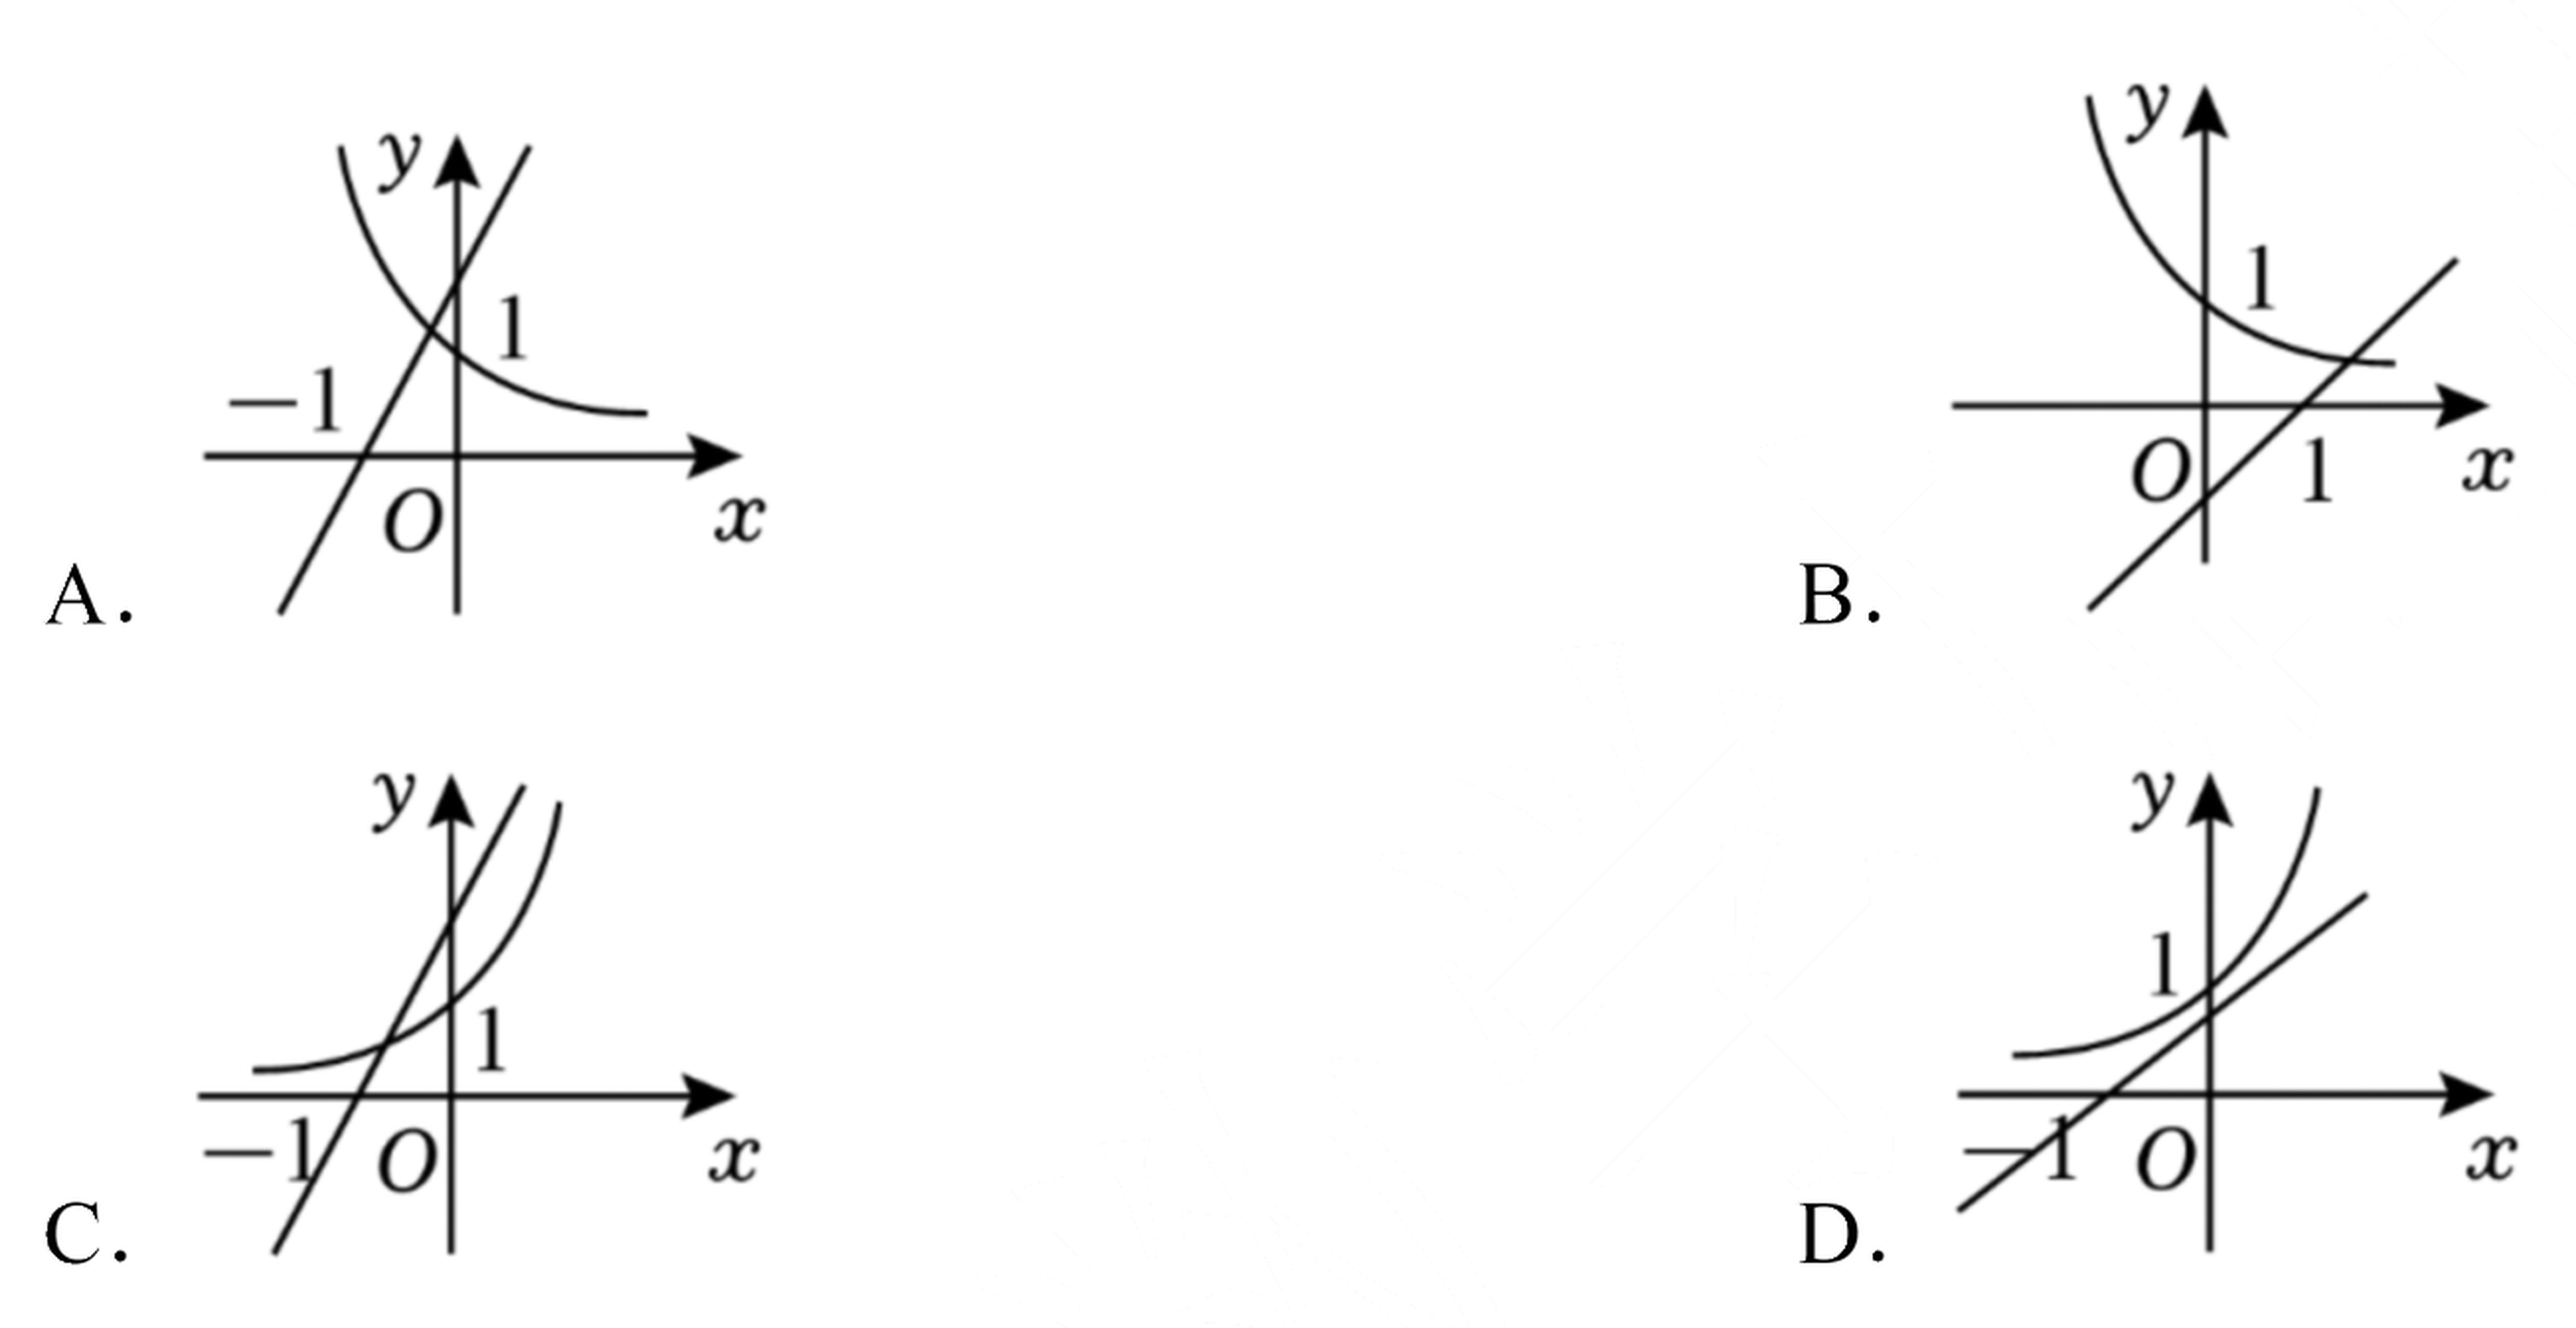
\includegraphics[width=0.80\textwidth]{figures/gao142_q15.png}
\end{center}

\ifanswer
\solbegin
\step{$A$ 中，由指数函数 $y=a^x(a>0\text{ 且 }a\neq1)$ 图像递减得 $0<a<1$，}
\step{而一次函数 $y=a(x+1)$ 的图像与 $y$ 轴交点纵坐标为 $a>1$，二者矛盾，}
\step{所以 $A$ 错；}
\step{由一次函数 $y=a(x+1)$ 的图像与 $x$ 轴交点横坐标为 $-1$，排除 $B$；}
\step{$C$ 中，由指数函数 $y=a^x(a>0\text{ 且 }a\neq1)$ 图像递减得 $a>1$，}% 原卷"递减得 a>1"自相矛盾（递减应得 0<a<1），照录
\step{而一次函数 $y=a(x+1)$ 的图像与 $y$ 轴交点纵坐标为 $a>1$，二者 $a$ 值吻合，}
\step{所以 $C$ 对；}
\step{$D$ 中，由一次函数 $y=a(x+1)$ 的图像得 $a=1$，与 $a>0$ 且 $a\neq1$ 矛盾，}
\step{所以 $D$ 错.}
\step{故选 $C$.}
\solend
\fi

\item 不等式 $\lvert x+1\rvert+\lvert 2-x\rvert\geqslant a^2-2a$ 恒成立，则 $a$ 的取值范围是\mbox{（\quad）}

\keepwithprev
A. $[-1,3]$\qquad B. $(-\infty,3]\cup[3,+\infty)$\qquad C. $(-\infty,3)$\qquad D. $(3,+\infty)$

\ifanswer
\solbegin
\step{因为 $\lvert x+1\rvert+\lvert 2-x\rvert\geqslant\lvert(x+1)+(2-x)\rvert=3$，}
\step{所以 $\lvert x+1\rvert+\lvert 2-x\rvert$ 的最小值为 3，}
\step{因为 $\lvert x+1\rvert+\lvert 2-x\rvert\geqslant a^2-2a$ 恒成立，所以只需 $a^2-2a\leqslant3$，所以 $-1\leqslant a\leqslant3$，}
\step{所以 $a$ 的取值范围为 $[-1,3]$. 故选 $A$.}
\solend
\fi

\end{enumerate}

\bigsec{三、解答题}

\begin{enumerate}
\setcounter{enumi}{16}

\item 已知集合 $A=\left\{x\mid\dfrac{x-3}{x-1}\leqslant0\right\}$，$B=\{x\mid\lvert x-1\rvert<a\}$.

(1) 若 $a=1$，求 $A\cap B$；

(2) 若 $x\in A$ 是 $x\in B$ 的充分条件，求 $a$ 的取值范围.

\ifanswer
\solbegin
\step{(1) 不等式 $\dfrac{x-3}{x-1}\leqslant0$，等价于 $(x-3)(x-1)\leqslant0$ 且 $x-1\neq0$，解得 $1<x\leqslant3$，}
\step{所以 $A=\{x\mid 1<x\leqslant3\}$，}
\step{当 $a=1$ 时，不等式 $\lvert x-1\rvert<a$ 可化为 $\lvert x-1\rvert<1$，所以 $-1<x-1<1$，}
\step{故 $0<x<2$，所以 $B=\{x\mid 0<x<2\}$，}
\step{所以 $A\cap B=\{x\mid 1<x<2\}$；}
\step{(2) 因为 $x\in A$ 是 $x\in B$ 的充分条件，所以 $A\subseteq B$，}% 子集符号原卷印带下划线 $\subseteq$，照录
\step{因为 $A=\{x\mid 1<x\leqslant3\}\neq\varnothing$，所以 $B\neq\varnothing$，故 $a>0$，}
\step{由不等式 $\lvert x-1\rvert<a$，解得 $1-a<x<1+a$，}
\step{所以 $B=\{x\mid 1-a<x<1+a\}$，所以 $\begin{cases}1-a\leqslant1\\1+a>3\end{cases}$，解得 $a>2$，}
\step{所以 $a$ 的取值范围为 $(2,+\infty)$.}
\solend
\fi

\item 计算下列式子的值（请务必书写必要的计算步骤）

(1) $27^{\frac13}+\left(\dfrac76\right)^0+\sqrt{(3-\pi)^2}$；

(2) $\lg25+\lg4+7^{\log_7 2}-\log_2 3\times\log_3 4+\log_3 9$.

\ifanswer
\solbegin
\step{(1) $27^{\frac13}+\left(\dfrac76\right)^0+\sqrt{(3-\pi)^2}=3^{3\times\frac13}+1+\lvert 3-\pi\rvert=3+1+\pi-3=\pi+1$；}
\step{(2) 原式 $=\lg(25\times4)+2-\dfrac{\lg3}{\lg2}\times\dfrac{\lg4}{\lg3}+2=\lg100+2-\dfrac{2\lg2}{\lg2}+2$}
\step{$=2+2-2+2=4$.}
\solend
\fi

\item 已知关于 $x$ 的不等式 $mx^2-(3m^2-m+2)x+6m-2\geqslant0$.

(1) 当 $m=2$ 时，求关于 $x$ 的不等式的解集；

(2) 当 $m>0$ 时，求关于 $x$ 的不等式的解集.

\ifanswer
\solbegin
\step{(1) $m=2$ 时，不等式为 $x^2-6x+5\geqslant0$，即 $(x-1)(x-5)\geqslant0$，}
\step{解得 $x\leqslant1$ 或 $x\geqslant5$，所以不等式的解集是 $\{x\mid x\leqslant1$ 或 $x\geqslant5\}$.}
\step{(2) $m>0$ 时，不等式可化为 $(mx-2)[x-(3m-1)]\geqslant0$，}
\step{即 $\left(x-\dfrac2m\right)[x-(3m-1)]\geqslant0$，}
\step{若 $m=1$，则不等式为 $(x-2)^2\geqslant0$，解得 $x\in\R$；}
\step{若 $0<m<1$，则 $\dfrac2m>3m-1$，解不等式得 $x\geqslant\dfrac2m$ 或 $x\leqslant3m-1$；}
\step{若 $m>1$，则 $\dfrac2m<3m-1$，解不等式得 $x\geqslant3m-1$ 或 $x\leqslant\dfrac2m$；}
\step{综上，$0<m<1$ 时，不等式的解集是 $\{x\mid x\leqslant3m-1$ 或 $x\geqslant\dfrac2m\}$；}
\step{$m=1$ 时，不等式的解集为 $\R$；}
\step{$m>1$ 时，不等式的解集是 $\{x\mid x\leqslant\dfrac2m$ 或 $x\geqslant3m-1\}$.}
\solend
\fi

\item 如图，某人计划用篱笆围成一个一边靠墙（墙足够长）的矩形菜园. 设菜园的长为 $x$ 米，宽为 $y$ 米.

\begin{center}
% 矩形围栏示意图取原卷 07 页截图去粉色水印、去色、LANCZOS 放大；题目配图，三版都出
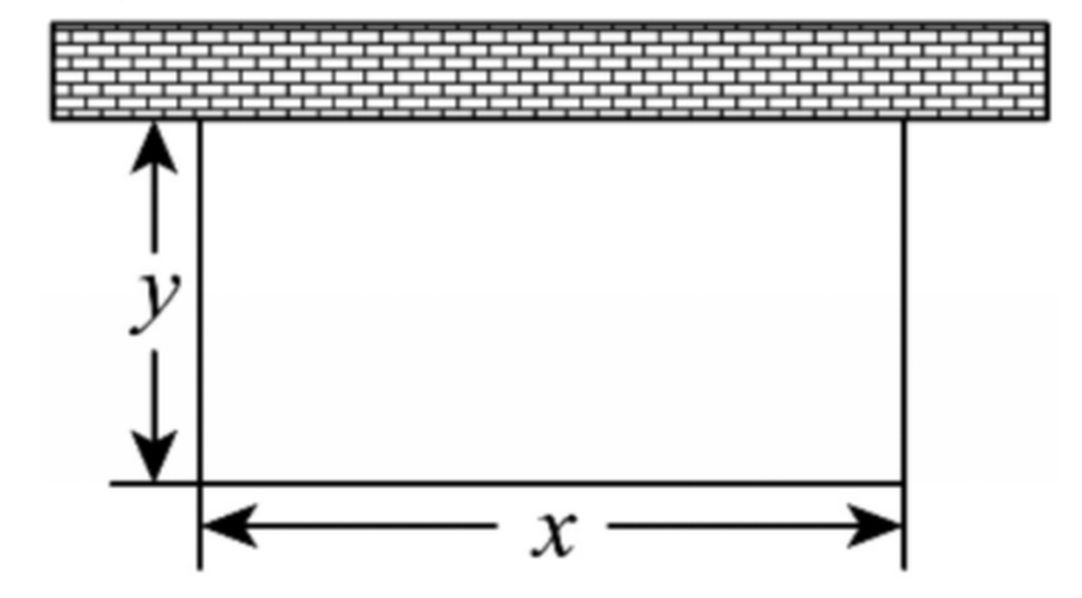
\includegraphics[width=0.42\textwidth]{figures/gao142_q20.png}
\end{center}

(1) 若菜园面积为 72 平方米，则 $x$、$y$ 为何值时，所用篱笆总长最小？

(2) 若 $x$、$y$ 满足 $x+y-xy+63=0$，则菜园面积最小为多少平方米？

\ifanswer
\solbegin
\step{(1) 由题意得，菜园的面积 $S=xy=72$，且 $x>0$，$y>0$，}
\step{所用篱笆总长 $L=x+2y$，}
\step{由基本不等式得 $x+2y\geqslant2\sqrt{x\cdot2y}=2\sqrt{2xy}=2\sqrt{2\times72}=24$，}
\step{当且仅当 $x=2y$ 时取等号，}
\step{联立 $\begin{cases}xy=72\\x=2y\end{cases}$，解得 $\begin{cases}x=12\\y=6\end{cases}$，}
\step{所以当 $x=12$，$y=6$ 时，所用篱笆总长最小；}
\step{(2) 由题意得 $x>0$，$y>0$，且满足 $x+y-xy+63=0$，即 $x+y=xy-63$，}
\step{由基本不等式得 $x+y\geqslant2\sqrt{xy}$，当且仅当 $x=y$ 时取等号，}
\step{所以 $xy-63\geqslant2\sqrt{xy}$. 令 $t=\sqrt{xy}(t>0)$，则 $xy=t^2$，}
\step{上述不等式可化为 $t^2-2t-63\geqslant0$，即 $(t-9)(t+7)\geqslant0$，}
\step{因为 $t>0$，所以 $t+7>0$，故 $t-9\geqslant0$，解得 $t\geqslant9$，所以 $\sqrt{xy}\geqslant9$，}
\step{即 $xy\geqslant81$，当且仅当 $x=y=9$ 时取等号，此时满足 $9+9-81+63=0$，}
\step{所以菜园面积最小为 81 平方米.}
\solend
\fi

\item 已知幂函数 $f(x)=(m^2-3m+3)x^m$ 的图象关于 $y$ 轴对称.

(1) 求实数 $m$ 的值；

(2) 在平面直角坐标系中作出函数 $y=\lvert f(x)-1\rvert$ 的图象；

(3) 已知点 $A(2a,y_1)$ 与点 $B(3-a,y_2)$ 都在幂函数 $y=x^2$ 的图象上. 若 $y_1<y_2$，求实数 $a$ 的取值范围.

\begin{center}
% 空白坐标网格取原卷 08 页截图去粉色水印、去色、LANCZOS 放大；题目配图，三版都出
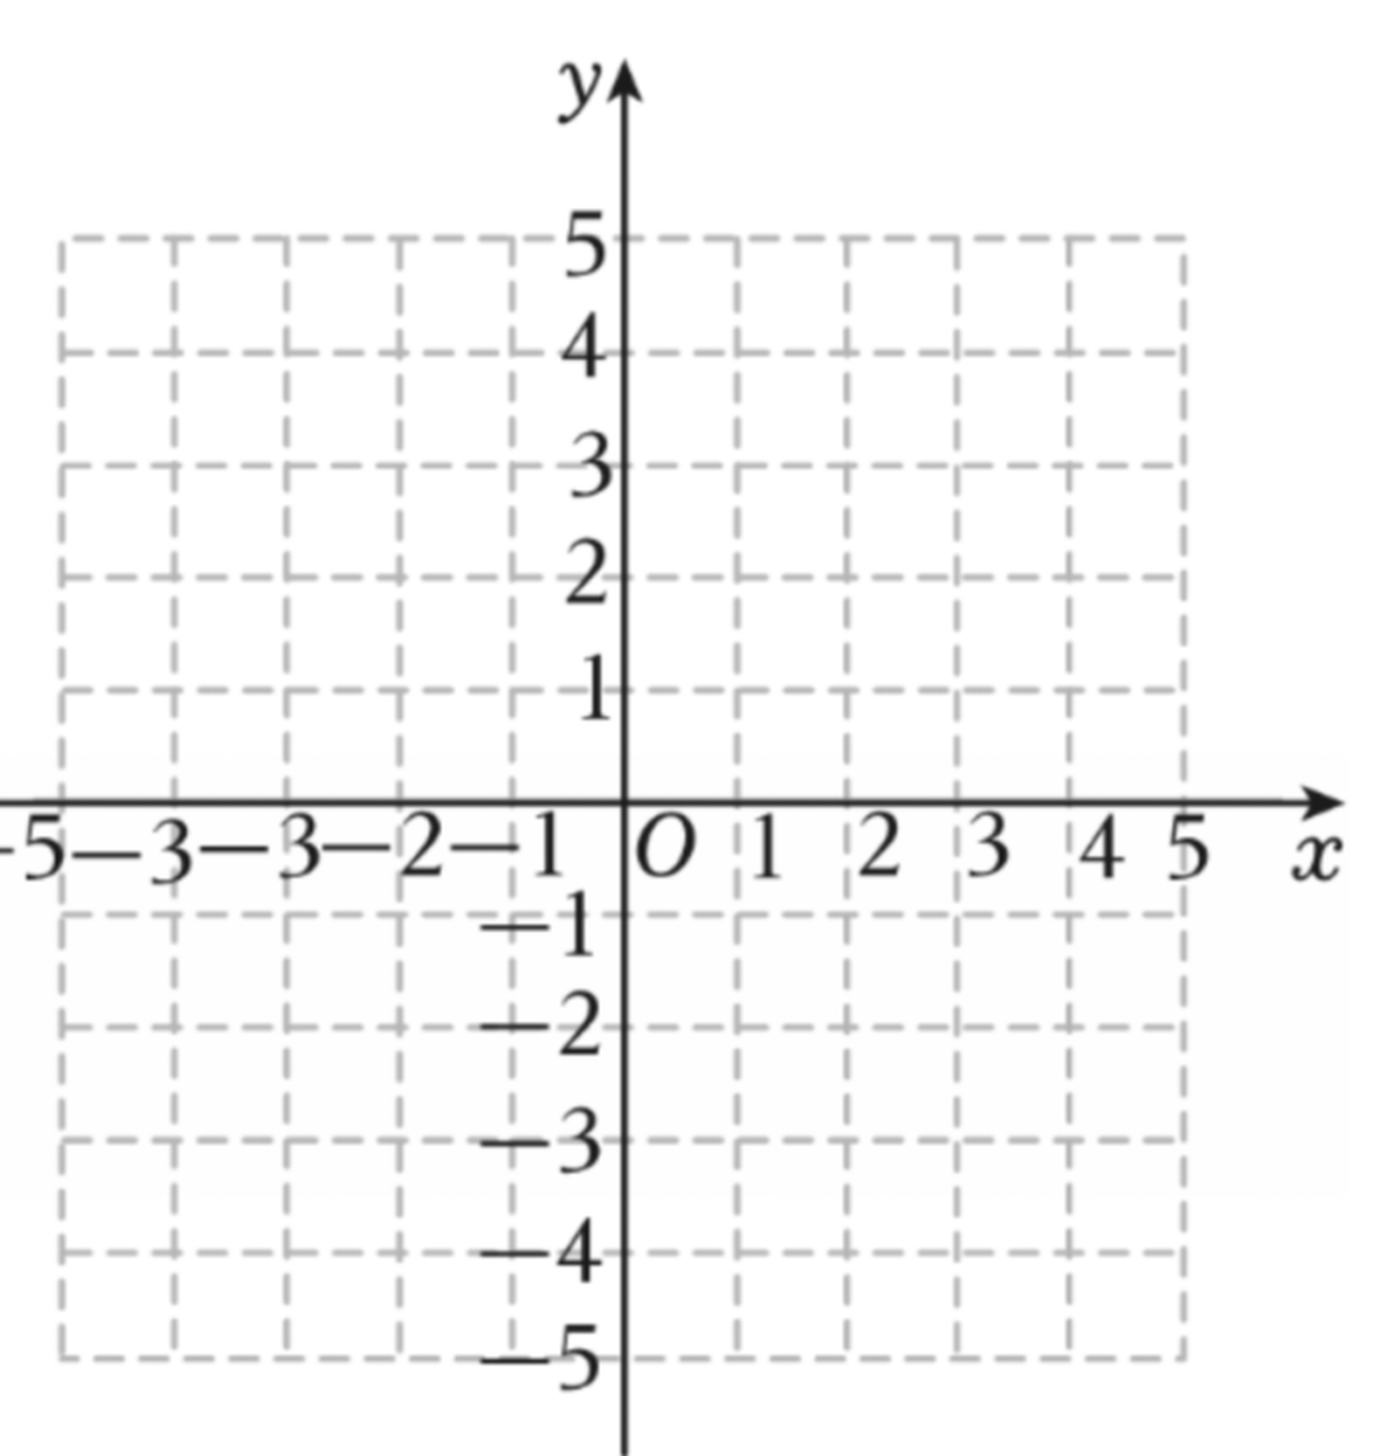
\includegraphics[width=0.52\textwidth]{figures/gao142_q21_grid.png}
\end{center}

\ifanswer
\solbegin
\step{(1) 由题意幂函数 $f(x)=(m^2-3m+3)x^m$，}
\step{故 $m^2-3m+3=1$，解得 $m=1$ 或 $m=2$，}
\step{又 $f(x)$ 图象关于 $y$ 轴对称，即 $f(x)$ 是偶函数，}
\step{当 $m=1$ 时，$f(x)=x$ 是奇函数，不满足条件，舍去；}
\step{当 $m=2$ 时，$f(x)=x^2$ 是偶函数，满足条件，故 $m=2$；}
\step{(2) 由 (1) 得，$\lvert f(x)-1\rvert=\lvert x^2-1\rvert$，}
\step{先画 $y=x^2-1$，开口向上的抛物线，顶点 $(0,-1)$，零点 $x=\pm1$，}
\step{再将 $x$ 轴下方的部分沿 $x$ 轴翻折到上方即为 $y=\lvert x^2-1\rvert$ 的图象，}
\step{图象如图所示.}
\par{\leftskip=0pt
\begin{center}
% 抛物线图象取原卷 09 页截图去粉色水印、去色、LANCZOS 放大；解析所附配图，仅答案版出
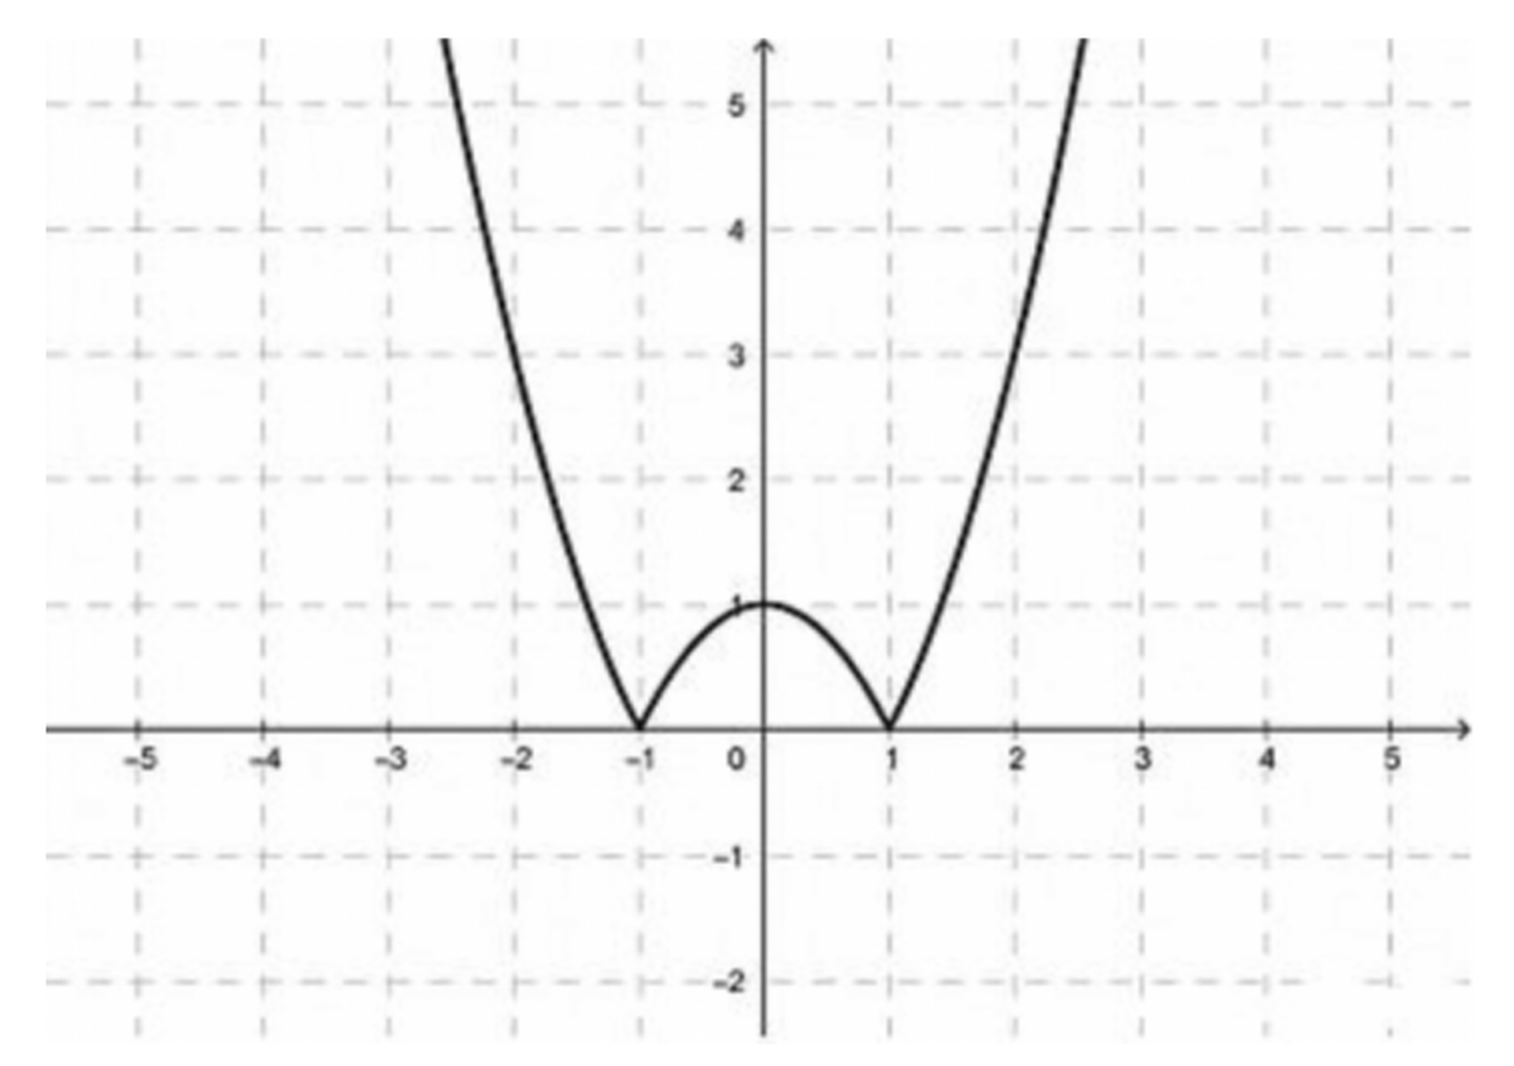
\includegraphics[width=0.55\textwidth]{figures/gao142_q21_para.png}
\end{center}}
\step{(3) 由题意得，$y_1=(2a)^2$，$y_2=(3-a)^2$，}
\step{$y_1<y_2$，即有 $(2a)^2<(3-a)^2$，化简整理得 $(a+3)(a-1)<0$，}
\step{解得实数 $a$ 的取值范围为 $(-3,1)$.}
\solend
\fi

\end{enumerate}

\end{document}
"
% 紧凑版：xelatex "\def\iscompact{1}% 高一142_群峰高级中学_期中.tex
%   —— 高一上数学"2026-2027 年群峰高级中学高一上期中"（试卷版/答案版）
% 试卷版：xelatex 高一142_群峰高级中学_期中.tex
% 答案版：xelatex "\def\isanswer{1}\input{高一142_群峰高级中学_期中.tex}"
% 紧凑版：xelatex "\def\iscompact{1}\input{高一142_群峰高级中学_期中.tex}"
%
% ① 原始材料：微信公众号"魔都数学加油站"文章，连载"27学年高一142"，原文标题
% "27学年高一142——2026-2027年上海市群峰高级中学高一上期中"；
% 原文链接：https://mp.weixin.qq.com/s/cc7wnuP4Pk3OjNDV6ihB9A。
% 正文为 9 张 PNG 页（01、02、04、06、07、08、09 为 2560x3620；03、05 为 4762x6735，
% 同一篇各页分辨率不同，逐页按各自分辨率裁图核对），题目下印有【答案】或【解析】，为讲评版。
% 题目、解析均据原图转录；卷面粉红色水印"魔都数学加油站"及公众号页脚未录入。
% 全卷 4 幅插图：第 15 题四幅坐标函数图像选项（04 页，2x2 合并为一张）、
% 第 20 题矩形围栏示意图（07 页）、第 21 题 (2) 空白坐标网格（08 页）、
% 第 21 题抛物线图象（09 页，解析所附图）；均取原卷截图去粉色水印、LANCZOS 放大。
% 题目配图三版都出、解析配图仅答案版出。
%
% 卷首标题：原卷印作"2026-2027 年群峰高级中学高一上期中"（公众号标题中的"上海市"
% 卷面标题行没有，本稿照卷面），年份区间按全稿惯例排 en dash；原卷未印副标题，
% 本卷为期中卷、跨集合与常用逻辑用语／不等式／函数三章，按题目内容补出
% "集合与常用逻辑用语、不等式、函数"（头注说明，与同期中卷口径相同）。
%
% 题号体例：本卷共 19 题——一、填空题 3—12（10 题）、二、选择题 13—16（4 题）、
% 三、解答题 17—21（5 题）。三节分别 \setcounter{enumi}{2}／{12}／{16}。
% 原卷从第 3 题起、无第 1、2 题，本稿保留原题号。
%
% ② 与原卷的排版差异：
%   ① 原文从第 3 题起，本稿保留原题号；原卷未印副标题，本稿按"知识模块"口径补出；
%   ② 逐题答案口径：Q14 原卷把答案 D 印在题干括号内、且题目下无【解析】，本稿括号
%      留空 \mbox{（\quad）}、另提 \ans{D}；Q13／Q15／Q16 答案在【解析】末句"故选 …"
%      （分别为 C／C／A），题干括号留空、不另提 \ans{}；其余各题（Q3—Q12、
%      Q17—Q21）题目下印【解析】、答案融在解析中，不另提 \ans{}；全卷仅 Q14 一处 \ans{}；
%      答案版【答案】/【解析】标记数 = 19（1 个 \ans + 18 个 \solbegin）= 全卷题数；
%   ③ 原卷填空横线按全稿惯例排 \blankline[4.4em]；选择题括号排 \mbox{（\quad）}、
%      每个选项段前按惯例加 \keepwithprev（Q15 四幅图那一枚放在 \begin{center} 之前）；
%      解答题不留作答区、不加 \anspace（原卷为讲评版，与 129／131／132／133／136／140 同）；
%   ④ 原卷数集斜体 $R$（Q5、Q7、Q19、Q21 解析等）按全稿惯例统一改 \R；空集记号
%      \varnothing；绝对值排 \lvert…\rvert，集合描述竖线排 \mid；不等号按全稿惯例
%      排 \leqslant／\geqslant；
%   ⑤ 4 幅插图：Q15 四幅坐标函数图象选项合并裁为一张 \includegraphics（题前
%      \needvspace{9cm}）；Q15 是"二、选择题"节内带大图块的第 3 题（Q13、Q14 在前
%      且无图），另在 \bigsec{二、选择题} 之前加 \needvspace{11cm} 连节标题一起量
%      ——守卫必须放在 \bigsec 之前，放标题之后会让"二、选择题"孤立在页末
%      （B 类，照 高一26／40／59／136／140 成例）；Q20 围栏图与 Q21 网格图置于题干
%      之后（三版都出），Q21 抛物线图置于答案版解析 (2) 与 (3) 之间（仅答案版出）；
%   ⑥ 子题标号按原卷排半角 (1)(2)(3)（与 140／141 同期中卷口径相同）；括注全角／
%      半角逐处照录：Q3"（用含有 m 的代数式表示）"、Q6"（舍）"、Q10"（万元）"、
%      Q18"（请务必书写必要的计算步骤）"、Q20"（墙足够长）"印全角；Q15
%      "$y=a^x(a>0 且 a\neq1)$"、Q10"$y=x^a(a 为常数)$"、Q20"$t=\sqrt{xy}(t>0)$"
%      等数学式内括注印半角；数学式内 CJK 用 \text{…}（否则 FONTCHK 报缺字）；
%   ⑦ 数学式内半角逗号照录（如 Q6"$ax-1=0,a\in\R$"、Q9"$b=2+\sqrt2,a=\sqrt2+1$"、
%      Q16 区间 "$[-1,3]$"、Q21"$y_1<y_2$，即 $(2a)^2<(3-a)^2$" 等）；原卷行末
%      西文句点照录（Q7"(-3,5)."、Q10"125（万元）."、Q19 题干句点、Q20 题干
%      "矩形菜园."与"宽为 y 米."、Q21 题干"对称." 等）；行中全角逗号、分号照录；
%   ⑧ 题干中的中文弯引号：本卷题干与解析通篇未出现中文弯引号，故无此项；
%      圈数字 ①②③ 亦未出现（子题用 (1)(2)(3)）；
%   ⑨ 原卷"图像／图象"两种写法混用，逐处放大核对并照录：Q4 题干与解析作"图象"、
%      Q7 解析作"图象"、Q8 题干作"图像"而解析作"图象"、Q15 题干与解析通篇作
%      "图像"、Q21 题干与解析通篇作"图象"；
%   ⑩ 原卷无红色加粗标签（【解析】均黑色印刷；逐页扫描深红像素为 0），故本卷未用
%      \stepm；黑色常规分步标签（"A 中""C 中""D 中""(1)(2)(3)" 等）按普通 \step
%      行内文字照录；
%   ⑪ 跨页续印按题合并，明细见 ⑥。
%
% ③ 行数复核：一条 \step = 原卷解析的一个印刷行，cases 块作一个印刷行计。逐题数 \step
%   条数，合计 98 条（Q3：1；Q4：2；Q5：3；Q6：4；Q7：5；Q8：2；Q9：4；Q10：3；
%   Q11：4；Q12：3；Q13：5；Q14：0；Q15：10；Q16：4；Q17：10；Q18：3；
%   Q19：10；Q20：13；Q21：12），与原卷印刷行逐题相等。Q14 只把答案印在题干括号、
%   无【解析】，提 \ans{D}、不计入 \step 账；答案版标记数 = 19（1 个 \ans + 18 个
%   \solbegin）= 全卷题数。
%
% ④ 判别式字形：全卷判别式共 3 处——第 7 题【解析】"即判别式△<0"、
%   "即△=(a-1)^2-4×1×4<0" 两处原卷印扁等边三角 $\triangle$，
%   第 11 题【解析】cases 块"△=4a^2-4(a+6)≥0" 一处原卷印等腰偏高的高三角 $\Delta$；
%   逐处放大核对，两形不同、全卷混用，本稿逐处照录不统一（参照 高一141 头注④口径）。
%   子集符号：全卷共 3 处——第 6 题题干"若 B⊆A"、第 6 题【解析】"因为 B⊆A"、
%   第 17 题【解析】(2)"所以 A⊆B"，逐处放大核对，原卷三处均印带下划线的
%   $\subseteq$（不是单线 $\subset$），本稿一律照录 \subseteq；全卷未出现 \subset。
%
% ⑤ 原卷存疑照录（均照录未改，正文对应处另有 % 注）：
%   第 14 题题干括号内原卷印答案 D（非留空），且题目下无【解析】，按"答案印括号且
%      无解析"口径括号留空、另提 \ans{D}；
%   第 15 题【解析】"C 中，由指数函数 … 图像递减得 a>1" 中"递减"与"a>1"
%      自相矛盾（递减应得 0<a<1，疑为"递增"之误），照录；
%   第 16 题选项 B 作 $(-\infty,3]\cup[3,+\infty)$，两端区间并起即全体实数、
%      与正确答案 $[-1,3]$ 不成干扰项（疑为 $(-\infty,-1]\cup[3,+\infty)$ 之误），照录；
%   第 21 题 (2) 空白坐标网格的 x 轴刻度原卷印作"-5 -3 -3 -2 -1 0 1 2 3 4 5"
%      （"-3"重复，疑为"-4"之误），系插图中的印刷内容，取原卷截图照录、不改图。
%
% ⑥ 跨页续印说明：Q7 题干与解析首行在 01 页、解析续至 02 页；Q11 题干与解析
%   4 行在 03 页；Q13 解析前 4 行在 03 页、末句"故选 C."续至 04 页；Q15 题干与
%   四幅图在 04 页、解析前 8 行在 04 页、末 2 行续至 05 页；Q17 解析前 7 行在
%   05 页、后 3 行续至 06 页；Q19 解析前 5 行在 06 页、后 5 行续至 07 页；
%   Q20 解析前 9 行在 07 页、后 4 行续至 08 页；Q21 解析 (1)(2) 9 行在 08 页、
%   抛物线图与 (3) 3 行续至 09 页；本稿按题连排，不丢行。三版切页审计结论见
%   编译自验回报（切页守卫见 ②⑤）。
%
\documentclass[a4paper,11pt]{article}
\usepackage{common}

\begin{document}

\examtitlest[3]{2026--2027 年群峰高级中学高一上期中}{集合与常用逻辑用语、不等式、函数}

\bigsec{一、填空题}

\begin{enumerate}
\setcounter{enumi}{2}

\item 已知 $\log_2 3=m$，则 $\log_3 6=$\blankline[4.4em]（用含有 $m$ 的代数式表示）.

\ifanswer
\solbegin
\step{$\log_3 6=\dfrac{\log_2 6}{\log_2 3}=\dfrac{\log_2 2+\log_2 3}{\log_2 3}=\dfrac{1+m}{m}=\dfrac1m+1$.}
\solend
\fi

\item 若指数函数 $y=a^x$ 的图象经过点 $(3,27)$，则 $a$ 的值为\blankline[4.4em].

\ifanswer
\solbegin
\step{因为指数函数 $y=a^x$ 的图象经过点 $(3,27)$，}
\step{所以 $a^3=27=3^3$，所以 $a=3$.}
\solend
\fi

\item 不等式 $(2x+1)^{\frac13}<(3-x)^{\frac13}$ 的解集为\blankline[4.4em].

\ifanswer
\solbegin
\step{因为幂函数 $f(t)=t^{\frac13}$ 在 $\R$ 上严格增，}
\step{所以原不等式等价于 $2x+1<3-x$，解得 $x<\dfrac23$，}
\step{因此原不等式的解集为 $\left(-\infty,\dfrac23\right)$.}
\solend
\fi

\item 设集合 $A=\{1,-2\}$，$B=\{x\mid ax-1=0,a\in\R\}$，若 $B\subseteq A$，则 $a$ 的值为\blankline[4.4em].% 子集符号原卷印带下划线 $\subseteq$，照录

\ifanswer
\solbegin
\step{因为 $B\subseteq A$，所以 $B=\varnothing$ 或 $\{-2\}$ 或 $\{1\}$ 或 $\{1,-2\}$（舍），}% 子集符号原卷印带下划线 $\subseteq$，照录
\step{若 $B=\varnothing$，则 $a=0$；若 $B=\{1\}$，则 $a=1$；}
\step{若 $B=\{-2\}$，则 $-2a=1$，解得 $a=-\dfrac12$；}
\step{综上，$a=0$ 或 $1$ 或 $-\dfrac12$.}
\solend
\fi

\item 不等式 $x^2+(a-1)x+4>0$ 在 $\R$ 上恒成立，则实数 $a$ 的取值范围是\blankline[4.4em].

\ifanswer
\solbegin
\step{不等式 $x^2+(a-1)x+4>0$，对应的二次函数为 $y=x^2+(a-1)x+4$，}
\step{因此函数图象开口向上，要使不等式对任意实数 $x$ 恒成立，}
\step{需二次函数图象与 $x$ 轴无交点，即判别式 $\triangle<0$，}% 判别式原卷印扁等边三角 $\triangle$，照录
\step{即 $\triangle=(a-1)^2-4\times1\times4<0$，整理得 $a^2-2a-15<0$，}% 判别式原卷印扁等边三角 $\triangle$，照录
\step{解得 $-3<a<5$，故实数 $a$ 的取值范围是 $(-3,5)$.}
\solend
\fi

\item 函数 $f(x)=(5x-3)^a$ 的图像恒过点\blankline[4.4em].% 题干作"图像"、解析作"图象"，原卷混用，逐处照录

\ifanswer
\solbegin
\step{令 $5x-3=1$ 得 $x=\dfrac45$，此时 $f\left(\dfrac45\right)=\left(5\times\dfrac45-3\right)^a=1$，}
\step{所以 $f(x)$ 的图象恒过 $\left(\dfrac45,1\right)$.}
\solend
\fi

\item 若 $a>0$，$b>0$ 且 $\dfrac1a+\dfrac2b=1$，则 $a+b$ 的最小值为\blankline[4.4em].

\ifanswer
\solbegin
\step{因为 $a>0$，$b>0$，$\dfrac1a+\dfrac2b=1$，}
\step{所以 $a+b=(a+b)\left(\dfrac1a+\dfrac2b\right)=1+\dfrac{2a}{b}+\dfrac{b}{a}+2\geqslant3+2\sqrt{\dfrac{2a}{b}\cdot\dfrac{b}{a}}=3+2\sqrt2$，}
\step{当且仅当 $\dfrac{2a}{b}=\dfrac{b}{a}$，即 $b=2+\sqrt2,a=\sqrt2+1$ 时取等号，}
\step{故 $a+b$ 的最小值为 $3+2\sqrt2$.}
\solend
\fi

\item 某药厂研制出一种新型药剂，投放市场后其广告投入 $x$（万元）与药品利润 $y$（万元）存在的关系为 $y=x^a(a\text{ 为常数})$，其中 $x$ 不超过 5 万元. 已知去年投入广告费用为 3 万元时，药品利润为 27 万元，若今年投入广告费用 5 万元，预计今年药品利润为\blankline[4.4em]万元.

\ifanswer
\solbegin
\step{由已知投入广告费用为 3 万元时，药品利润为 27 万元，}
\step{代入 $y=x^a$ 中，即 $3^a=27$，解得 $a=3$，故函数关系式为 $y=x^3$，}
\step{所以当 $x=5$ 时，$y=125$（万元）.}
\solend
\fi

\item 已知方程 $x^2+2ax+a+6=0$ 的两根分别是 $x_1$ 和 $x_2$，且满足 $\dfrac1{x_1}+\dfrac1{x_2}<0$，则实数 $a$ 的取值范围是\blankline[4.4em].

\ifanswer
\solbegin
\step{由于方程 $x^2+2ax+a+6=0$ 的两根分别是 $x_1$ 和 $x_2$，}
\step{则 $\begin{cases}\Delta=4a^2-4(a+6)\geqslant0\\x_1+x_2=-2a\\x_1x_2=a+6\end{cases}$，解得 $a\geqslant3$ 或 $a\leqslant-2$.}% 判别式原卷印等腰偏高的高三角 $\Delta$，照录（与第 7 题扁等边 $\triangle$ 两形混用）
\step{又 $\dfrac1{x_1}+\dfrac1{x_2}<0$，即 $\dfrac{x_1+x_2}{x_1\cdot x_2}<0$，故 $\dfrac{-2a}{a+6}<0$，解得 $a<-6$ 或 $a>0$.}
\step{综上，$a$ 的取值范围是 $(-\infty,-6)\cup[3,+\infty)$.}
\solend
\fi

\item 已知 $b>a>1$，若 $\log_a b-\log_b a=\dfrac32$，$a^b=b^a$，则 $a-b=$\blankline[4.4em].

\ifanswer
\solbegin
\step{因为 $b>a>1$，所以 $\log_a b>1$，}
\step{由 $\log_a b-\log_b a=\log_a b-\dfrac{1}{\log_a b}=\dfrac32$，解得 $\log_a b=2$ 即 $b=a^2$，}
\step{因为 $a^b=b^a=a^{2a}$，所以 $b=2a=a^2$，所以 $a=2$，$b=4$，则 $a-b=-2$.}
\solend
\fi

\end{enumerate}

% 第 15 题四幅图是"二、选择题"节内的大图块；守卫须放在 \bigsec 之前连节标题一起量
\needvspace{11cm}
\bigsec{二、选择题}

\begin{enumerate}
\setcounter{enumi}{12}

\item 若 $a>b$，$c<0$，则下列不等式正确的是\mbox{（\quad）}

\keepwithprev
A. $ab>bc$\qquad B. $a+c<b+c$\qquad C. $ac^2>bc^2$\qquad D. $\dfrac ac>\dfrac bc$

\ifanswer
\solbegin
\step{因为 $a>b$，$c<0$，取 $b=0$，则 $ab=bc=0$，故 $A$ 错误；}
\step{由于 $a>b$，所以 $a+c>b+c$，故 $B$ 错误；}
\step{由 $c<0$ 得 $c^2>0$，所以 $ac^2>bc^2$，故 $C$ 正确；}
\step{由于 $a>b$ 且 $c<0$，所以 $\dfrac ac<\dfrac bc$，故 $D$ 错误.}
\step{故选 $C$.}
\solend
\fi

\item 若 $x>0$，$y>0$，则下列各式中，恒成立的是\mbox{（\quad）}% 原卷题干括号内印答案 D、且题目下无【解析】，本稿括号留空、另提 \ans{D}

\keepwithprev
A. $\lg x+\lg y=\lg(x+y)$\qquad B. $\lg x^2=(\lg x)^2$

C. $\dfrac{\lg x}{\lg y}=\lg(x-y)$\qquad D. $\lg x^{\frac1n}=\dfrac{\lg x}{n}$

\ifanswer
\ans{$D$}
\fi

% 第 15 题四幅坐标函数图象选项是一整块，守卫放在 \item 之前
\needvspace{9cm}
\item 在同一平面直角坐标系中，指数函数 $y=a^x(a>0\text{ 且 }a\neq1)$ 和一次函数 $y=a(x+1)$ 的图像关系可能是\mbox{（\quad）}

\keepwithprev
\begin{center}
% 四幅坐标函数图象选项取原卷 04 页截图去粉色水印、去色，按原卷 2x2 排布合并为一张
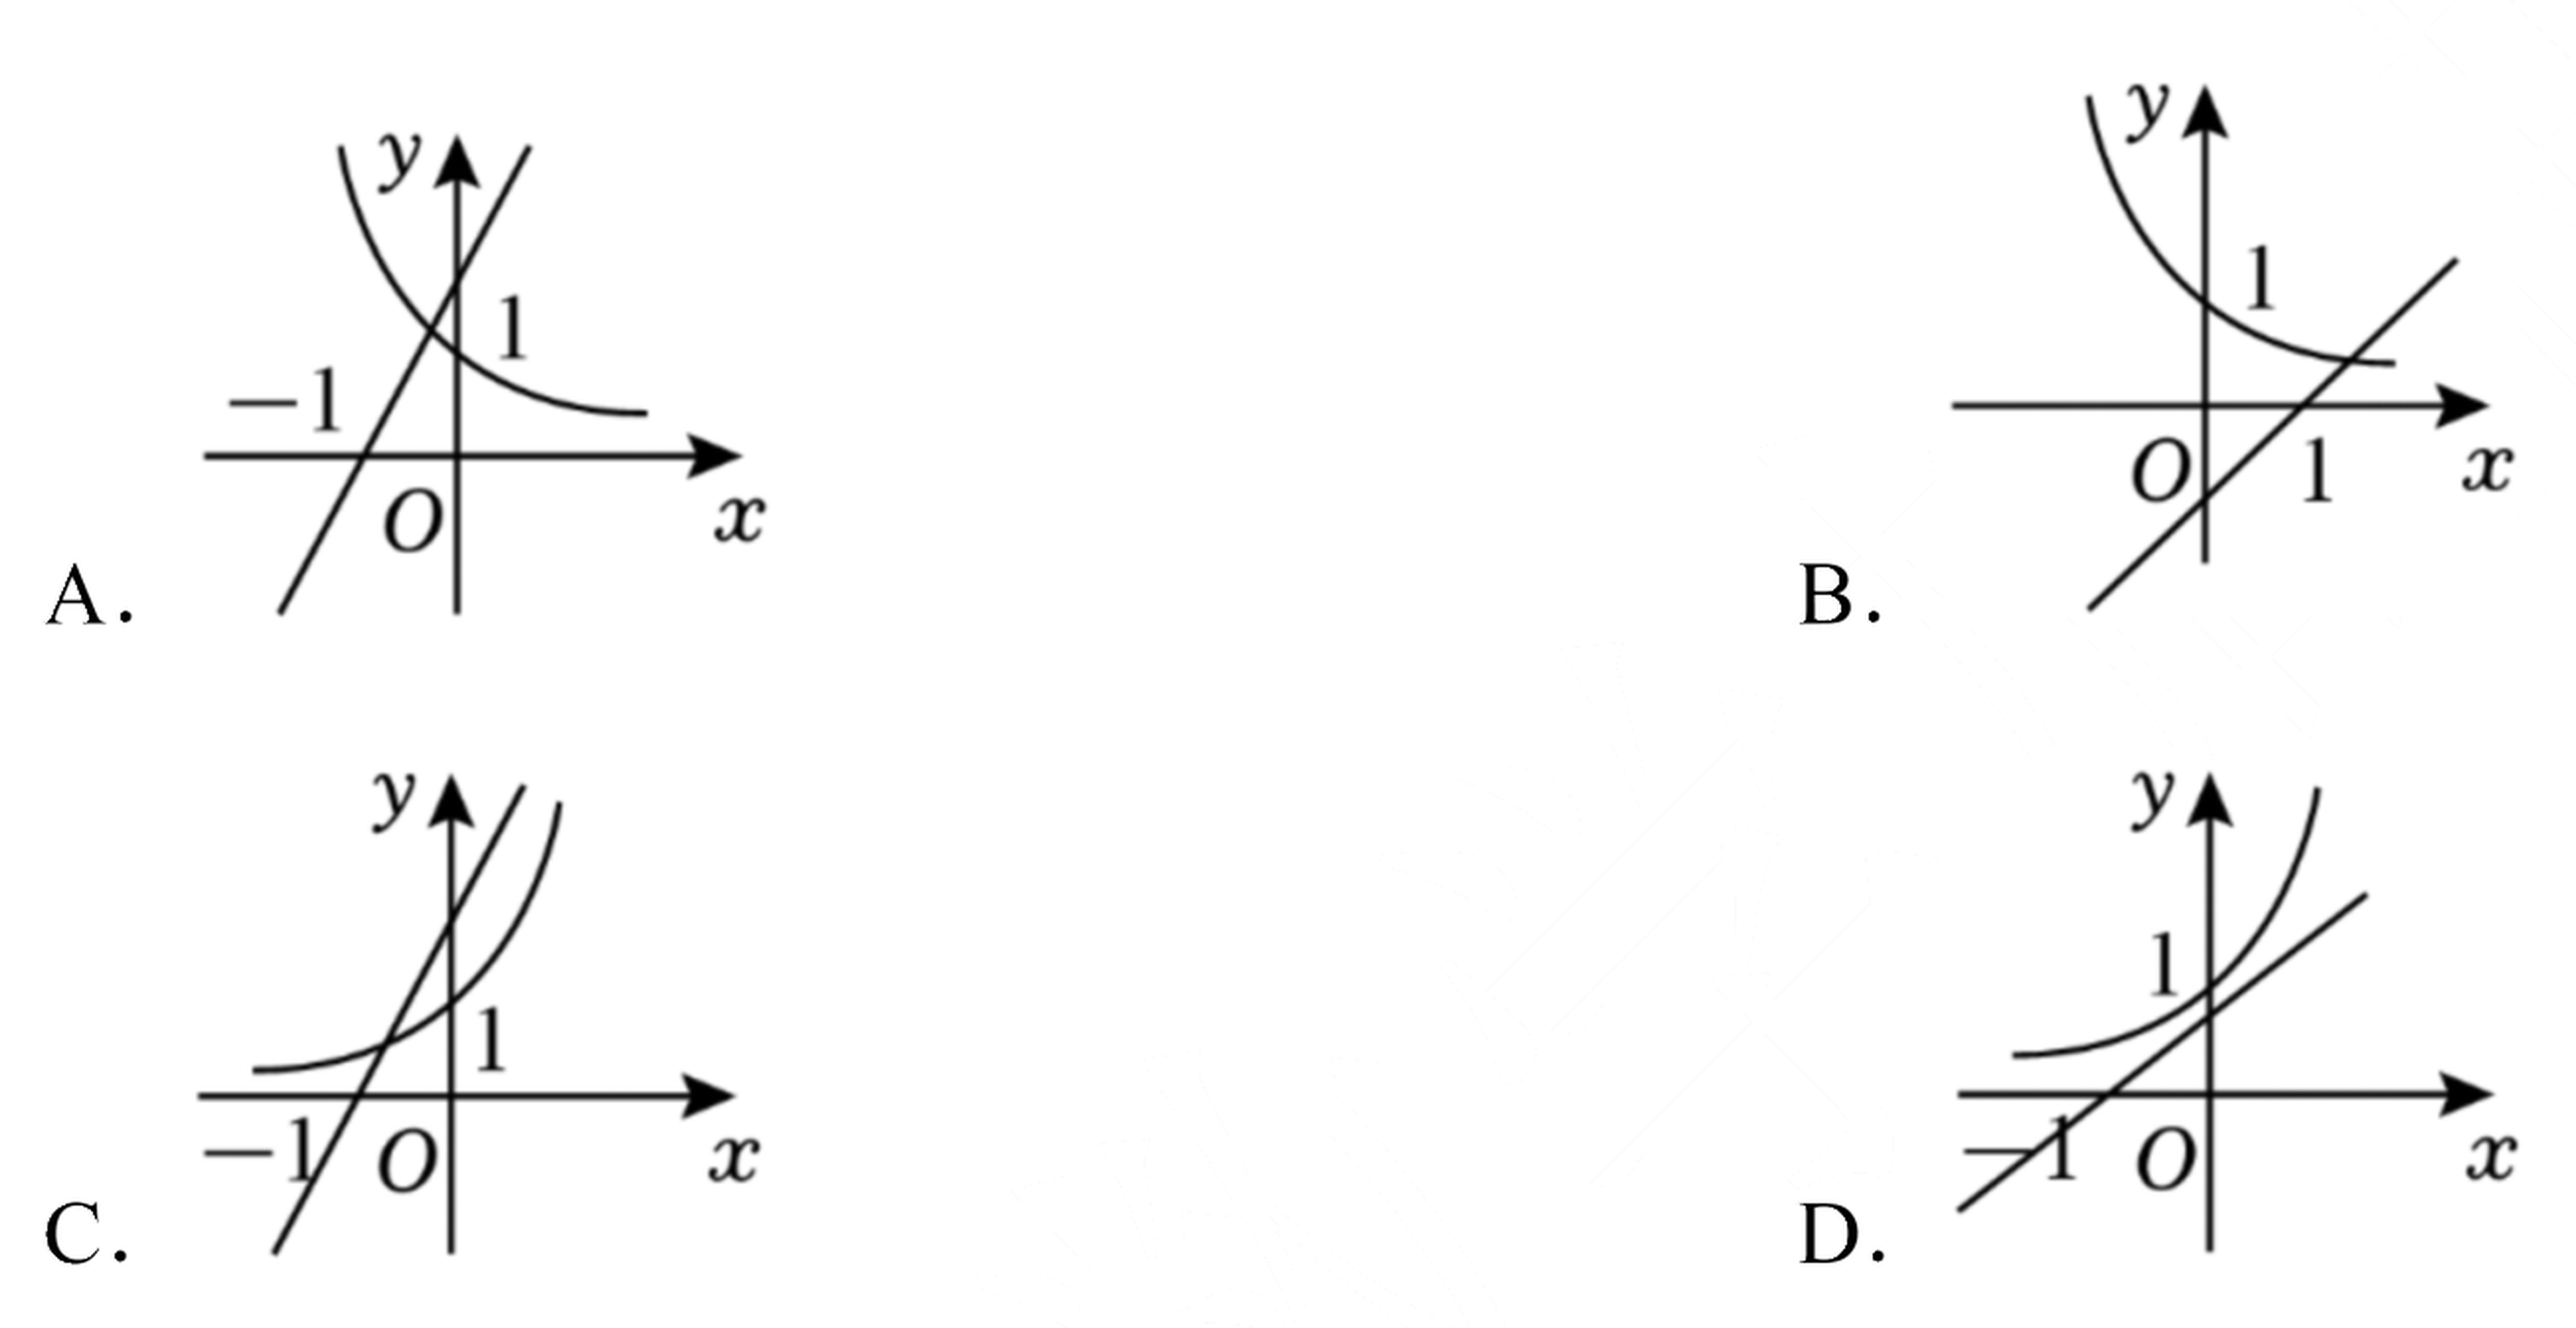
\includegraphics[width=0.80\textwidth]{figures/gao142_q15.png}
\end{center}

\ifanswer
\solbegin
\step{$A$ 中，由指数函数 $y=a^x(a>0\text{ 且 }a\neq1)$ 图像递减得 $0<a<1$，}
\step{而一次函数 $y=a(x+1)$ 的图像与 $y$ 轴交点纵坐标为 $a>1$，二者矛盾，}
\step{所以 $A$ 错；}
\step{由一次函数 $y=a(x+1)$ 的图像与 $x$ 轴交点横坐标为 $-1$，排除 $B$；}
\step{$C$ 中，由指数函数 $y=a^x(a>0\text{ 且 }a\neq1)$ 图像递减得 $a>1$，}% 原卷"递减得 a>1"自相矛盾（递减应得 0<a<1），照录
\step{而一次函数 $y=a(x+1)$ 的图像与 $y$ 轴交点纵坐标为 $a>1$，二者 $a$ 值吻合，}
\step{所以 $C$ 对；}
\step{$D$ 中，由一次函数 $y=a(x+1)$ 的图像得 $a=1$，与 $a>0$ 且 $a\neq1$ 矛盾，}
\step{所以 $D$ 错.}
\step{故选 $C$.}
\solend
\fi

\item 不等式 $\lvert x+1\rvert+\lvert 2-x\rvert\geqslant a^2-2a$ 恒成立，则 $a$ 的取值范围是\mbox{（\quad）}

\keepwithprev
A. $[-1,3]$\qquad B. $(-\infty,3]\cup[3,+\infty)$\qquad C. $(-\infty,3)$\qquad D. $(3,+\infty)$

\ifanswer
\solbegin
\step{因为 $\lvert x+1\rvert+\lvert 2-x\rvert\geqslant\lvert(x+1)+(2-x)\rvert=3$，}
\step{所以 $\lvert x+1\rvert+\lvert 2-x\rvert$ 的最小值为 3，}
\step{因为 $\lvert x+1\rvert+\lvert 2-x\rvert\geqslant a^2-2a$ 恒成立，所以只需 $a^2-2a\leqslant3$，所以 $-1\leqslant a\leqslant3$，}
\step{所以 $a$ 的取值范围为 $[-1,3]$. 故选 $A$.}
\solend
\fi

\end{enumerate}

\bigsec{三、解答题}

\begin{enumerate}
\setcounter{enumi}{16}

\item 已知集合 $A=\left\{x\mid\dfrac{x-3}{x-1}\leqslant0\right\}$，$B=\{x\mid\lvert x-1\rvert<a\}$.

(1) 若 $a=1$，求 $A\cap B$；

(2) 若 $x\in A$ 是 $x\in B$ 的充分条件，求 $a$ 的取值范围.

\ifanswer
\solbegin
\step{(1) 不等式 $\dfrac{x-3}{x-1}\leqslant0$，等价于 $(x-3)(x-1)\leqslant0$ 且 $x-1\neq0$，解得 $1<x\leqslant3$，}
\step{所以 $A=\{x\mid 1<x\leqslant3\}$，}
\step{当 $a=1$ 时，不等式 $\lvert x-1\rvert<a$ 可化为 $\lvert x-1\rvert<1$，所以 $-1<x-1<1$，}
\step{故 $0<x<2$，所以 $B=\{x\mid 0<x<2\}$，}
\step{所以 $A\cap B=\{x\mid 1<x<2\}$；}
\step{(2) 因为 $x\in A$ 是 $x\in B$ 的充分条件，所以 $A\subseteq B$，}% 子集符号原卷印带下划线 $\subseteq$，照录
\step{因为 $A=\{x\mid 1<x\leqslant3\}\neq\varnothing$，所以 $B\neq\varnothing$，故 $a>0$，}
\step{由不等式 $\lvert x-1\rvert<a$，解得 $1-a<x<1+a$，}
\step{所以 $B=\{x\mid 1-a<x<1+a\}$，所以 $\begin{cases}1-a\leqslant1\\1+a>3\end{cases}$，解得 $a>2$，}
\step{所以 $a$ 的取值范围为 $(2,+\infty)$.}
\solend
\fi

\item 计算下列式子的值（请务必书写必要的计算步骤）

(1) $27^{\frac13}+\left(\dfrac76\right)^0+\sqrt{(3-\pi)^2}$；

(2) $\lg25+\lg4+7^{\log_7 2}-\log_2 3\times\log_3 4+\log_3 9$.

\ifanswer
\solbegin
\step{(1) $27^{\frac13}+\left(\dfrac76\right)^0+\sqrt{(3-\pi)^2}=3^{3\times\frac13}+1+\lvert 3-\pi\rvert=3+1+\pi-3=\pi+1$；}
\step{(2) 原式 $=\lg(25\times4)+2-\dfrac{\lg3}{\lg2}\times\dfrac{\lg4}{\lg3}+2=\lg100+2-\dfrac{2\lg2}{\lg2}+2$}
\step{$=2+2-2+2=4$.}
\solend
\fi

\item 已知关于 $x$ 的不等式 $mx^2-(3m^2-m+2)x+6m-2\geqslant0$.

(1) 当 $m=2$ 时，求关于 $x$ 的不等式的解集；

(2) 当 $m>0$ 时，求关于 $x$ 的不等式的解集.

\ifanswer
\solbegin
\step{(1) $m=2$ 时，不等式为 $x^2-6x+5\geqslant0$，即 $(x-1)(x-5)\geqslant0$，}
\step{解得 $x\leqslant1$ 或 $x\geqslant5$，所以不等式的解集是 $\{x\mid x\leqslant1$ 或 $x\geqslant5\}$.}
\step{(2) $m>0$ 时，不等式可化为 $(mx-2)[x-(3m-1)]\geqslant0$，}
\step{即 $\left(x-\dfrac2m\right)[x-(3m-1)]\geqslant0$，}
\step{若 $m=1$，则不等式为 $(x-2)^2\geqslant0$，解得 $x\in\R$；}
\step{若 $0<m<1$，则 $\dfrac2m>3m-1$，解不等式得 $x\geqslant\dfrac2m$ 或 $x\leqslant3m-1$；}
\step{若 $m>1$，则 $\dfrac2m<3m-1$，解不等式得 $x\geqslant3m-1$ 或 $x\leqslant\dfrac2m$；}
\step{综上，$0<m<1$ 时，不等式的解集是 $\{x\mid x\leqslant3m-1$ 或 $x\geqslant\dfrac2m\}$；}
\step{$m=1$ 时，不等式的解集为 $\R$；}
\step{$m>1$ 时，不等式的解集是 $\{x\mid x\leqslant\dfrac2m$ 或 $x\geqslant3m-1\}$.}
\solend
\fi

\item 如图，某人计划用篱笆围成一个一边靠墙（墙足够长）的矩形菜园. 设菜园的长为 $x$ 米，宽为 $y$ 米.

\begin{center}
% 矩形围栏示意图取原卷 07 页截图去粉色水印、去色、LANCZOS 放大；题目配图，三版都出
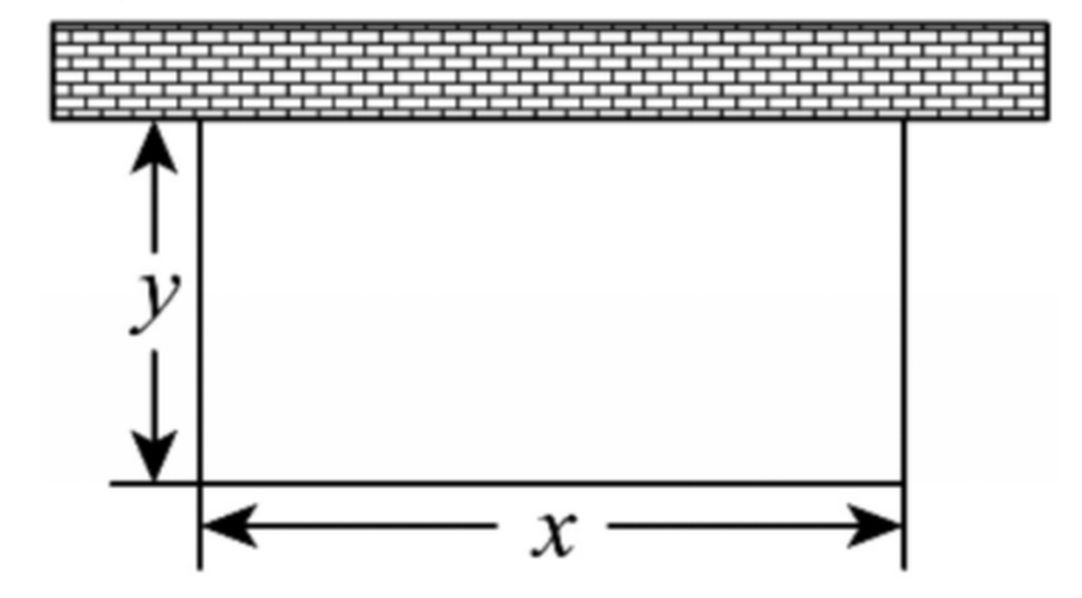
\includegraphics[width=0.42\textwidth]{figures/gao142_q20.png}
\end{center}

(1) 若菜园面积为 72 平方米，则 $x$、$y$ 为何值时，所用篱笆总长最小？

(2) 若 $x$、$y$ 满足 $x+y-xy+63=0$，则菜园面积最小为多少平方米？

\ifanswer
\solbegin
\step{(1) 由题意得，菜园的面积 $S=xy=72$，且 $x>0$，$y>0$，}
\step{所用篱笆总长 $L=x+2y$，}
\step{由基本不等式得 $x+2y\geqslant2\sqrt{x\cdot2y}=2\sqrt{2xy}=2\sqrt{2\times72}=24$，}
\step{当且仅当 $x=2y$ 时取等号，}
\step{联立 $\begin{cases}xy=72\\x=2y\end{cases}$，解得 $\begin{cases}x=12\\y=6\end{cases}$，}
\step{所以当 $x=12$，$y=6$ 时，所用篱笆总长最小；}
\step{(2) 由题意得 $x>0$，$y>0$，且满足 $x+y-xy+63=0$，即 $x+y=xy-63$，}
\step{由基本不等式得 $x+y\geqslant2\sqrt{xy}$，当且仅当 $x=y$ 时取等号，}
\step{所以 $xy-63\geqslant2\sqrt{xy}$. 令 $t=\sqrt{xy}(t>0)$，则 $xy=t^2$，}
\step{上述不等式可化为 $t^2-2t-63\geqslant0$，即 $(t-9)(t+7)\geqslant0$，}
\step{因为 $t>0$，所以 $t+7>0$，故 $t-9\geqslant0$，解得 $t\geqslant9$，所以 $\sqrt{xy}\geqslant9$，}
\step{即 $xy\geqslant81$，当且仅当 $x=y=9$ 时取等号，此时满足 $9+9-81+63=0$，}
\step{所以菜园面积最小为 81 平方米.}
\solend
\fi

\item 已知幂函数 $f(x)=(m^2-3m+3)x^m$ 的图象关于 $y$ 轴对称.

(1) 求实数 $m$ 的值；

(2) 在平面直角坐标系中作出函数 $y=\lvert f(x)-1\rvert$ 的图象；

(3) 已知点 $A(2a,y_1)$ 与点 $B(3-a,y_2)$ 都在幂函数 $y=x^2$ 的图象上. 若 $y_1<y_2$，求实数 $a$ 的取值范围.

\begin{center}
% 空白坐标网格取原卷 08 页截图去粉色水印、去色、LANCZOS 放大；题目配图，三版都出
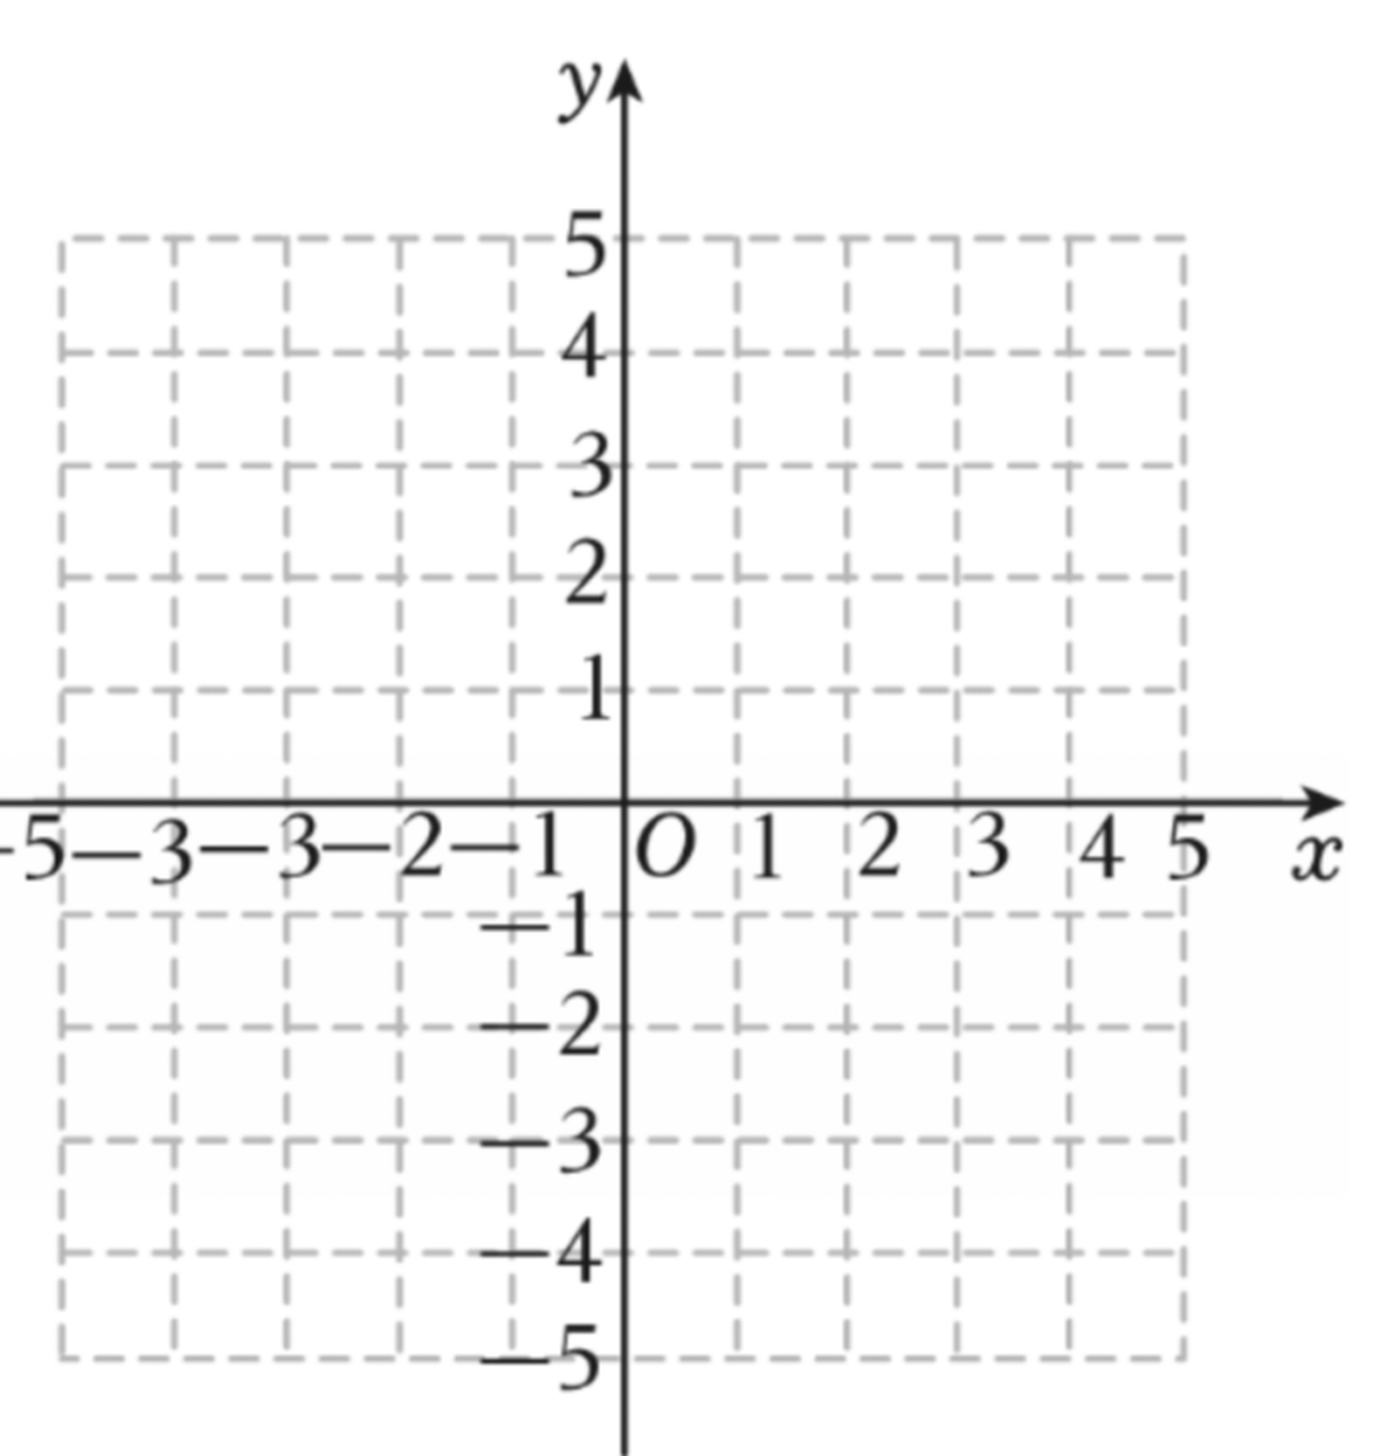
\includegraphics[width=0.52\textwidth]{figures/gao142_q21_grid.png}
\end{center}

\ifanswer
\solbegin
\step{(1) 由题意幂函数 $f(x)=(m^2-3m+3)x^m$，}
\step{故 $m^2-3m+3=1$，解得 $m=1$ 或 $m=2$，}
\step{又 $f(x)$ 图象关于 $y$ 轴对称，即 $f(x)$ 是偶函数，}
\step{当 $m=1$ 时，$f(x)=x$ 是奇函数，不满足条件，舍去；}
\step{当 $m=2$ 时，$f(x)=x^2$ 是偶函数，满足条件，故 $m=2$；}
\step{(2) 由 (1) 得，$\lvert f(x)-1\rvert=\lvert x^2-1\rvert$，}
\step{先画 $y=x^2-1$，开口向上的抛物线，顶点 $(0,-1)$，零点 $x=\pm1$，}
\step{再将 $x$ 轴下方的部分沿 $x$ 轴翻折到上方即为 $y=\lvert x^2-1\rvert$ 的图象，}
\step{图象如图所示.}
\par{\leftskip=0pt
\begin{center}
% 抛物线图象取原卷 09 页截图去粉色水印、去色、LANCZOS 放大；解析所附配图，仅答案版出
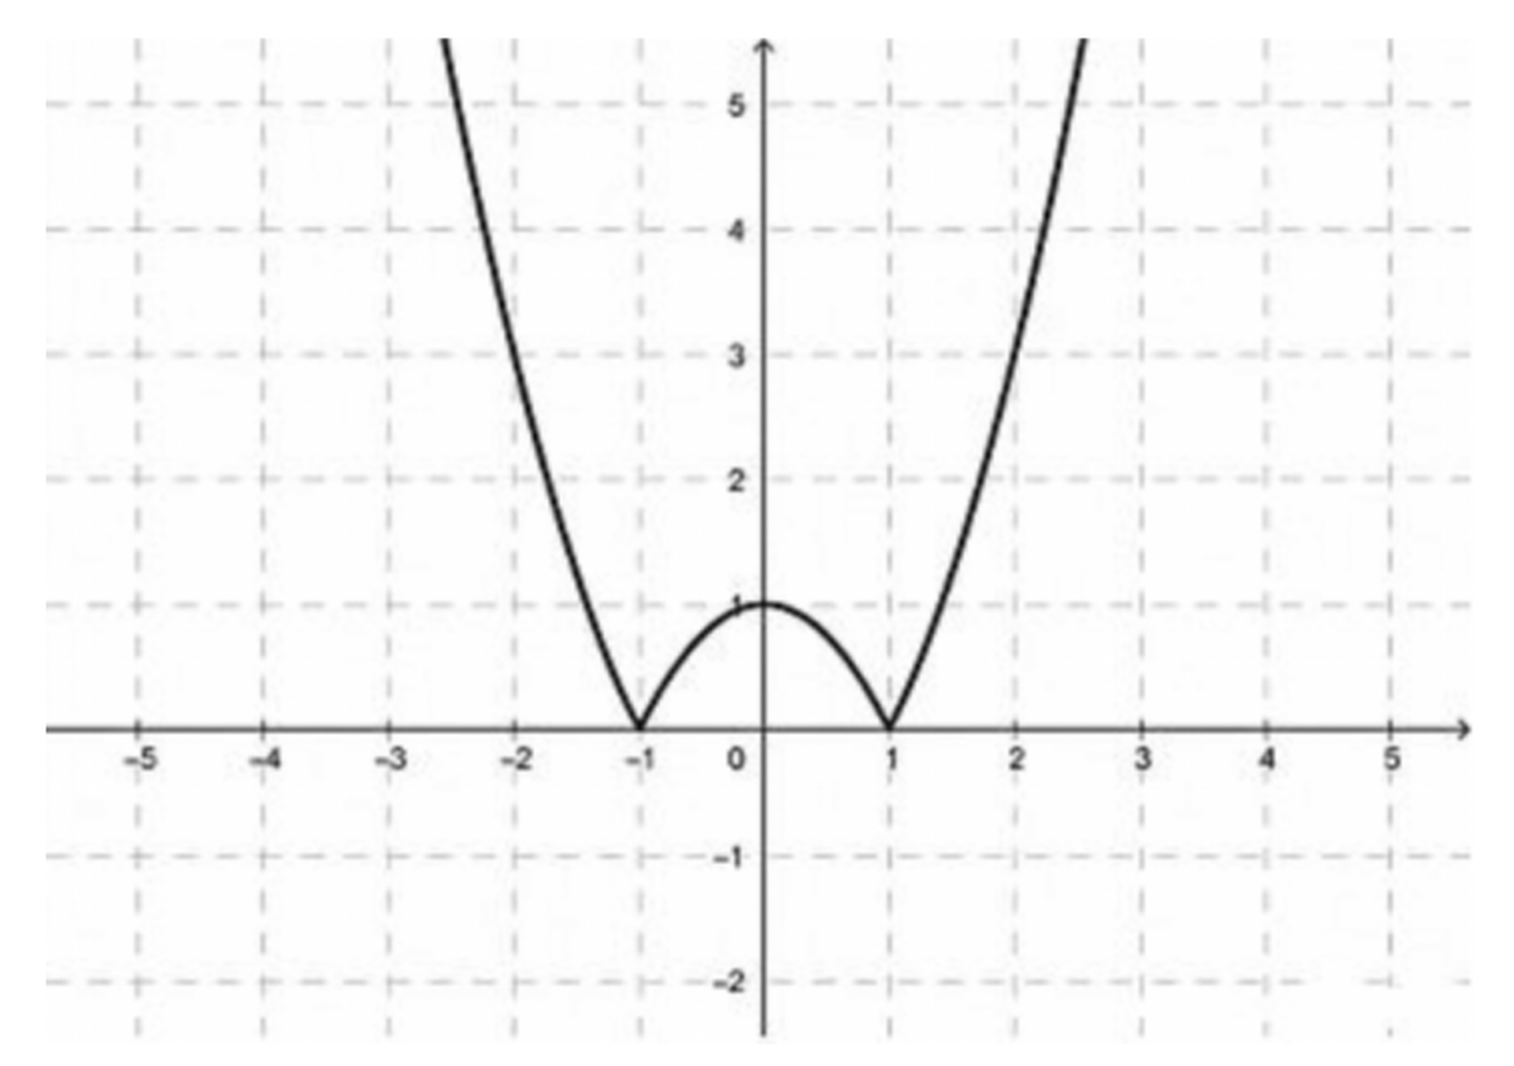
\includegraphics[width=0.55\textwidth]{figures/gao142_q21_para.png}
\end{center}}
\step{(3) 由题意得，$y_1=(2a)^2$，$y_2=(3-a)^2$，}
\step{$y_1<y_2$，即有 $(2a)^2<(3-a)^2$，化简整理得 $(a+3)(a-1)<0$，}
\step{解得实数 $a$ 的取值范围为 $(-3,1)$.}
\solend
\fi

\end{enumerate}

\end{document}
"
%
% ① 原始材料：微信公众号"魔都数学加油站"文章，连载"27学年高一142"，原文标题
% "27学年高一142——2026-2027年上海市群峰高级中学高一上期中"；
% 原文链接：https://mp.weixin.qq.com/s/cc7wnuP4Pk3OjNDV6ihB9A。
% 正文为 9 张 PNG 页（01、02、04、06、07、08、09 为 2560x3620；03、05 为 4762x6735，
% 同一篇各页分辨率不同，逐页按各自分辨率裁图核对），题目下印有【答案】或【解析】，为讲评版。
% 题目、解析均据原图转录；卷面粉红色水印"魔都数学加油站"及公众号页脚未录入。
% 全卷 4 幅插图：第 15 题四幅坐标函数图像选项（04 页，2x2 合并为一张）、
% 第 20 题矩形围栏示意图（07 页）、第 21 题 (2) 空白坐标网格（08 页）、
% 第 21 题抛物线图象（09 页，解析所附图）；均取原卷截图去粉色水印、LANCZOS 放大。
% 题目配图三版都出、解析配图仅答案版出。
%
% 卷首标题：原卷印作"2026-2027 年群峰高级中学高一上期中"（公众号标题中的"上海市"
% 卷面标题行没有，本稿照卷面），年份区间按全稿惯例排 en dash；原卷未印副标题，
% 本卷为期中卷、跨集合与常用逻辑用语／不等式／函数三章，按题目内容补出
% "集合与常用逻辑用语、不等式、函数"（头注说明，与同期中卷口径相同）。
%
% 题号体例：本卷共 19 题——一、填空题 3—12（10 题）、二、选择题 13—16（4 题）、
% 三、解答题 17—21（5 题）。三节分别 \setcounter{enumi}{2}／{12}／{16}。
% 原卷从第 3 题起、无第 1、2 题，本稿保留原题号。
%
% ② 与原卷的排版差异：
%   ① 原文从第 3 题起，本稿保留原题号；原卷未印副标题，本稿按"知识模块"口径补出；
%   ② 逐题答案口径：Q14 原卷把答案 D 印在题干括号内、且题目下无【解析】，本稿括号
%      留空 \mbox{（\quad）}、另提 \ans{D}；Q13／Q15／Q16 答案在【解析】末句"故选 …"
%      （分别为 C／C／A），题干括号留空、不另提 \ans{}；其余各题（Q3—Q12、
%      Q17—Q21）题目下印【解析】、答案融在解析中，不另提 \ans{}；全卷仅 Q14 一处 \ans{}；
%      答案版【答案】/【解析】标记数 = 19（1 个 \ans + 18 个 \solbegin）= 全卷题数；
%   ③ 原卷填空横线按全稿惯例排 \blankline[4.4em]；选择题括号排 \mbox{（\quad）}、
%      每个选项段前按惯例加 \keepwithprev（Q15 四幅图那一枚放在 \begin{center} 之前）；
%      解答题不留作答区、不加 \anspace（原卷为讲评版，与 129／131／132／133／136／140 同）；
%   ④ 原卷数集斜体 $R$（Q5、Q7、Q19、Q21 解析等）按全稿惯例统一改 \R；空集记号
%      \varnothing；绝对值排 \lvert…\rvert，集合描述竖线排 \mid；不等号按全稿惯例
%      排 \leqslant／\geqslant；
%   ⑤ 4 幅插图：Q15 四幅坐标函数图象选项合并裁为一张 \includegraphics（题前
%      \needvspace{9cm}）；Q15 是"二、选择题"节内带大图块的第 3 题（Q13、Q14 在前
%      且无图），另在 \bigsec{二、选择题} 之前加 \needvspace{11cm} 连节标题一起量
%      ——守卫必须放在 \bigsec 之前，放标题之后会让"二、选择题"孤立在页末
%      （B 类，照 高一26／40／59／136／140 成例）；Q20 围栏图与 Q21 网格图置于题干
%      之后（三版都出），Q21 抛物线图置于答案版解析 (2) 与 (3) 之间（仅答案版出）；
%   ⑥ 子题标号按原卷排半角 (1)(2)(3)（与 140／141 同期中卷口径相同）；括注全角／
%      半角逐处照录：Q3"（用含有 m 的代数式表示）"、Q6"（舍）"、Q10"（万元）"、
%      Q18"（请务必书写必要的计算步骤）"、Q20"（墙足够长）"印全角；Q15
%      "$y=a^x(a>0 且 a\neq1)$"、Q10"$y=x^a(a 为常数)$"、Q20"$t=\sqrt{xy}(t>0)$"
%      等数学式内括注印半角；数学式内 CJK 用 \text{…}（否则 FONTCHK 报缺字）；
%   ⑦ 数学式内半角逗号照录（如 Q6"$ax-1=0,a\in\R$"、Q9"$b=2+\sqrt2,a=\sqrt2+1$"、
%      Q16 区间 "$[-1,3]$"、Q21"$y_1<y_2$，即 $(2a)^2<(3-a)^2$" 等）；原卷行末
%      西文句点照录（Q7"(-3,5)."、Q10"125（万元）."、Q19 题干句点、Q20 题干
%      "矩形菜园."与"宽为 y 米."、Q21 题干"对称." 等）；行中全角逗号、分号照录；
%   ⑧ 题干中的中文弯引号：本卷题干与解析通篇未出现中文弯引号，故无此项；
%      圈数字 ①②③ 亦未出现（子题用 (1)(2)(3)）；
%   ⑨ 原卷"图像／图象"两种写法混用，逐处放大核对并照录：Q4 题干与解析作"图象"、
%      Q7 解析作"图象"、Q8 题干作"图像"而解析作"图象"、Q15 题干与解析通篇作
%      "图像"、Q21 题干与解析通篇作"图象"；
%   ⑩ 原卷无红色加粗标签（【解析】均黑色印刷；逐页扫描深红像素为 0），故本卷未用
%      \stepm；黑色常规分步标签（"A 中""C 中""D 中""(1)(2)(3)" 等）按普通 \step
%      行内文字照录；
%   ⑪ 跨页续印按题合并，明细见 ⑥。
%
% ③ 行数复核：一条 \step = 原卷解析的一个印刷行，cases 块作一个印刷行计。逐题数 \step
%   条数，合计 98 条（Q3：1；Q4：2；Q5：3；Q6：4；Q7：5；Q8：2；Q9：4；Q10：3；
%   Q11：4；Q12：3；Q13：5；Q14：0；Q15：10；Q16：4；Q17：10；Q18：3；
%   Q19：10；Q20：13；Q21：12），与原卷印刷行逐题相等。Q14 只把答案印在题干括号、
%   无【解析】，提 \ans{D}、不计入 \step 账；答案版标记数 = 19（1 个 \ans + 18 个
%   \solbegin）= 全卷题数。
%
% ④ 判别式字形：全卷判别式共 3 处——第 7 题【解析】"即判别式△<0"、
%   "即△=(a-1)^2-4×1×4<0" 两处原卷印扁等边三角 $\triangle$，
%   第 11 题【解析】cases 块"△=4a^2-4(a+6)≥0" 一处原卷印等腰偏高的高三角 $\Delta$；
%   逐处放大核对，两形不同、全卷混用，本稿逐处照录不统一（参照 高一141 头注④口径）。
%   子集符号：全卷共 3 处——第 6 题题干"若 B⊆A"、第 6 题【解析】"因为 B⊆A"、
%   第 17 题【解析】(2)"所以 A⊆B"，逐处放大核对，原卷三处均印带下划线的
%   $\subseteq$（不是单线 $\subset$），本稿一律照录 \subseteq；全卷未出现 \subset。
%
% ⑤ 原卷存疑照录（均照录未改，正文对应处另有 % 注）：
%   第 14 题题干括号内原卷印答案 D（非留空），且题目下无【解析】，按"答案印括号且
%      无解析"口径括号留空、另提 \ans{D}；
%   第 15 题【解析】"C 中，由指数函数 … 图像递减得 a>1" 中"递减"与"a>1"
%      自相矛盾（递减应得 0<a<1，疑为"递增"之误），照录；
%   第 16 题选项 B 作 $(-\infty,3]\cup[3,+\infty)$，两端区间并起即全体实数、
%      与正确答案 $[-1,3]$ 不成干扰项（疑为 $(-\infty,-1]\cup[3,+\infty)$ 之误），照录；
%   第 21 题 (2) 空白坐标网格的 x 轴刻度原卷印作"-5 -3 -3 -2 -1 0 1 2 3 4 5"
%      （"-3"重复，疑为"-4"之误），系插图中的印刷内容，取原卷截图照录、不改图。
%
% ⑥ 跨页续印说明：Q7 题干与解析首行在 01 页、解析续至 02 页；Q11 题干与解析
%   4 行在 03 页；Q13 解析前 4 行在 03 页、末句"故选 C."续至 04 页；Q15 题干与
%   四幅图在 04 页、解析前 8 行在 04 页、末 2 行续至 05 页；Q17 解析前 7 行在
%   05 页、后 3 行续至 06 页；Q19 解析前 5 行在 06 页、后 5 行续至 07 页；
%   Q20 解析前 9 行在 07 页、后 4 行续至 08 页；Q21 解析 (1)(2) 9 行在 08 页、
%   抛物线图与 (3) 3 行续至 09 页；本稿按题连排，不丢行。三版切页审计结论见
%   编译自验回报（切页守卫见 ②⑤）。
%
\documentclass[a4paper,11pt]{article}
\usepackage{common}

\begin{document}

\examtitlest[3]{2026--2027 年群峰高级中学高一上期中}{集合与常用逻辑用语、不等式、函数}

\bigsec{一、填空题}

\begin{enumerate}
\setcounter{enumi}{2}

\item 已知 $\log_2 3=m$，则 $\log_3 6=$\blankline[4.4em]（用含有 $m$ 的代数式表示）.

\ifanswer
\solbegin
\step{$\log_3 6=\dfrac{\log_2 6}{\log_2 3}=\dfrac{\log_2 2+\log_2 3}{\log_2 3}=\dfrac{1+m}{m}=\dfrac1m+1$.}
\solend
\fi

\item 若指数函数 $y=a^x$ 的图象经过点 $(3,27)$，则 $a$ 的值为\blankline[4.4em].

\ifanswer
\solbegin
\step{因为指数函数 $y=a^x$ 的图象经过点 $(3,27)$，}
\step{所以 $a^3=27=3^3$，所以 $a=3$.}
\solend
\fi

\item 不等式 $(2x+1)^{\frac13}<(3-x)^{\frac13}$ 的解集为\blankline[4.4em].

\ifanswer
\solbegin
\step{因为幂函数 $f(t)=t^{\frac13}$ 在 $\R$ 上严格增，}
\step{所以原不等式等价于 $2x+1<3-x$，解得 $x<\dfrac23$，}
\step{因此原不等式的解集为 $\left(-\infty,\dfrac23\right)$.}
\solend
\fi

\item 设集合 $A=\{1,-2\}$，$B=\{x\mid ax-1=0,a\in\R\}$，若 $B\subseteq A$，则 $a$ 的值为\blankline[4.4em].% 子集符号原卷印带下划线 $\subseteq$，照录

\ifanswer
\solbegin
\step{因为 $B\subseteq A$，所以 $B=\varnothing$ 或 $\{-2\}$ 或 $\{1\}$ 或 $\{1,-2\}$（舍），}% 子集符号原卷印带下划线 $\subseteq$，照录
\step{若 $B=\varnothing$，则 $a=0$；若 $B=\{1\}$，则 $a=1$；}
\step{若 $B=\{-2\}$，则 $-2a=1$，解得 $a=-\dfrac12$；}
\step{综上，$a=0$ 或 $1$ 或 $-\dfrac12$.}
\solend
\fi

\item 不等式 $x^2+(a-1)x+4>0$ 在 $\R$ 上恒成立，则实数 $a$ 的取值范围是\blankline[4.4em].

\ifanswer
\solbegin
\step{不等式 $x^2+(a-1)x+4>0$，对应的二次函数为 $y=x^2+(a-1)x+4$，}
\step{因此函数图象开口向上，要使不等式对任意实数 $x$ 恒成立，}
\step{需二次函数图象与 $x$ 轴无交点，即判别式 $\triangle<0$，}% 判别式原卷印扁等边三角 $\triangle$，照录
\step{即 $\triangle=(a-1)^2-4\times1\times4<0$，整理得 $a^2-2a-15<0$，}% 判别式原卷印扁等边三角 $\triangle$，照录
\step{解得 $-3<a<5$，故实数 $a$ 的取值范围是 $(-3,5)$.}
\solend
\fi

\item 函数 $f(x)=(5x-3)^a$ 的图像恒过点\blankline[4.4em].% 题干作"图像"、解析作"图象"，原卷混用，逐处照录

\ifanswer
\solbegin
\step{令 $5x-3=1$ 得 $x=\dfrac45$，此时 $f\left(\dfrac45\right)=\left(5\times\dfrac45-3\right)^a=1$，}
\step{所以 $f(x)$ 的图象恒过 $\left(\dfrac45,1\right)$.}
\solend
\fi

\item 若 $a>0$，$b>0$ 且 $\dfrac1a+\dfrac2b=1$，则 $a+b$ 的最小值为\blankline[4.4em].

\ifanswer
\solbegin
\step{因为 $a>0$，$b>0$，$\dfrac1a+\dfrac2b=1$，}
\step{所以 $a+b=(a+b)\left(\dfrac1a+\dfrac2b\right)=1+\dfrac{2a}{b}+\dfrac{b}{a}+2\geqslant3+2\sqrt{\dfrac{2a}{b}\cdot\dfrac{b}{a}}=3+2\sqrt2$，}
\step{当且仅当 $\dfrac{2a}{b}=\dfrac{b}{a}$，即 $b=2+\sqrt2,a=\sqrt2+1$ 时取等号，}
\step{故 $a+b$ 的最小值为 $3+2\sqrt2$.}
\solend
\fi

\item 某药厂研制出一种新型药剂，投放市场后其广告投入 $x$（万元）与药品利润 $y$（万元）存在的关系为 $y=x^a(a\text{ 为常数})$，其中 $x$ 不超过 5 万元. 已知去年投入广告费用为 3 万元时，药品利润为 27 万元，若今年投入广告费用 5 万元，预计今年药品利润为\blankline[4.4em]万元.

\ifanswer
\solbegin
\step{由已知投入广告费用为 3 万元时，药品利润为 27 万元，}
\step{代入 $y=x^a$ 中，即 $3^a=27$，解得 $a=3$，故函数关系式为 $y=x^3$，}
\step{所以当 $x=5$ 时，$y=125$（万元）.}
\solend
\fi

\item 已知方程 $x^2+2ax+a+6=0$ 的两根分别是 $x_1$ 和 $x_2$，且满足 $\dfrac1{x_1}+\dfrac1{x_2}<0$，则实数 $a$ 的取值范围是\blankline[4.4em].

\ifanswer
\solbegin
\step{由于方程 $x^2+2ax+a+6=0$ 的两根分别是 $x_1$ 和 $x_2$，}
\step{则 $\begin{cases}\Delta=4a^2-4(a+6)\geqslant0\\x_1+x_2=-2a\\x_1x_2=a+6\end{cases}$，解得 $a\geqslant3$ 或 $a\leqslant-2$.}% 判别式原卷印等腰偏高的高三角 $\Delta$，照录（与第 7 题扁等边 $\triangle$ 两形混用）
\step{又 $\dfrac1{x_1}+\dfrac1{x_2}<0$，即 $\dfrac{x_1+x_2}{x_1\cdot x_2}<0$，故 $\dfrac{-2a}{a+6}<0$，解得 $a<-6$ 或 $a>0$.}
\step{综上，$a$ 的取值范围是 $(-\infty,-6)\cup[3,+\infty)$.}
\solend
\fi

\item 已知 $b>a>1$，若 $\log_a b-\log_b a=\dfrac32$，$a^b=b^a$，则 $a-b=$\blankline[4.4em].

\ifanswer
\solbegin
\step{因为 $b>a>1$，所以 $\log_a b>1$，}
\step{由 $\log_a b-\log_b a=\log_a b-\dfrac{1}{\log_a b}=\dfrac32$，解得 $\log_a b=2$ 即 $b=a^2$，}
\step{因为 $a^b=b^a=a^{2a}$，所以 $b=2a=a^2$，所以 $a=2$，$b=4$，则 $a-b=-2$.}
\solend
\fi

\end{enumerate}

% 第 15 题四幅图是"二、选择题"节内的大图块；守卫须放在 \bigsec 之前连节标题一起量
\needvspace{11cm}
\bigsec{二、选择题}

\begin{enumerate}
\setcounter{enumi}{12}

\item 若 $a>b$，$c<0$，则下列不等式正确的是\mbox{（\quad）}

\keepwithprev
A. $ab>bc$\qquad B. $a+c<b+c$\qquad C. $ac^2>bc^2$\qquad D. $\dfrac ac>\dfrac bc$

\ifanswer
\solbegin
\step{因为 $a>b$，$c<0$，取 $b=0$，则 $ab=bc=0$，故 $A$ 错误；}
\step{由于 $a>b$，所以 $a+c>b+c$，故 $B$ 错误；}
\step{由 $c<0$ 得 $c^2>0$，所以 $ac^2>bc^2$，故 $C$ 正确；}
\step{由于 $a>b$ 且 $c<0$，所以 $\dfrac ac<\dfrac bc$，故 $D$ 错误.}
\step{故选 $C$.}
\solend
\fi

\item 若 $x>0$，$y>0$，则下列各式中，恒成立的是\mbox{（\quad）}% 原卷题干括号内印答案 D、且题目下无【解析】，本稿括号留空、另提 \ans{D}

\keepwithprev
A. $\lg x+\lg y=\lg(x+y)$\qquad B. $\lg x^2=(\lg x)^2$

C. $\dfrac{\lg x}{\lg y}=\lg(x-y)$\qquad D. $\lg x^{\frac1n}=\dfrac{\lg x}{n}$

\ifanswer
\ans{$D$}
\fi

% 第 15 题四幅坐标函数图象选项是一整块，守卫放在 \item 之前
\needvspace{9cm}
\item 在同一平面直角坐标系中，指数函数 $y=a^x(a>0\text{ 且 }a\neq1)$ 和一次函数 $y=a(x+1)$ 的图像关系可能是\mbox{（\quad）}

\keepwithprev
\begin{center}
% 四幅坐标函数图象选项取原卷 04 页截图去粉色水印、去色，按原卷 2x2 排布合并为一张
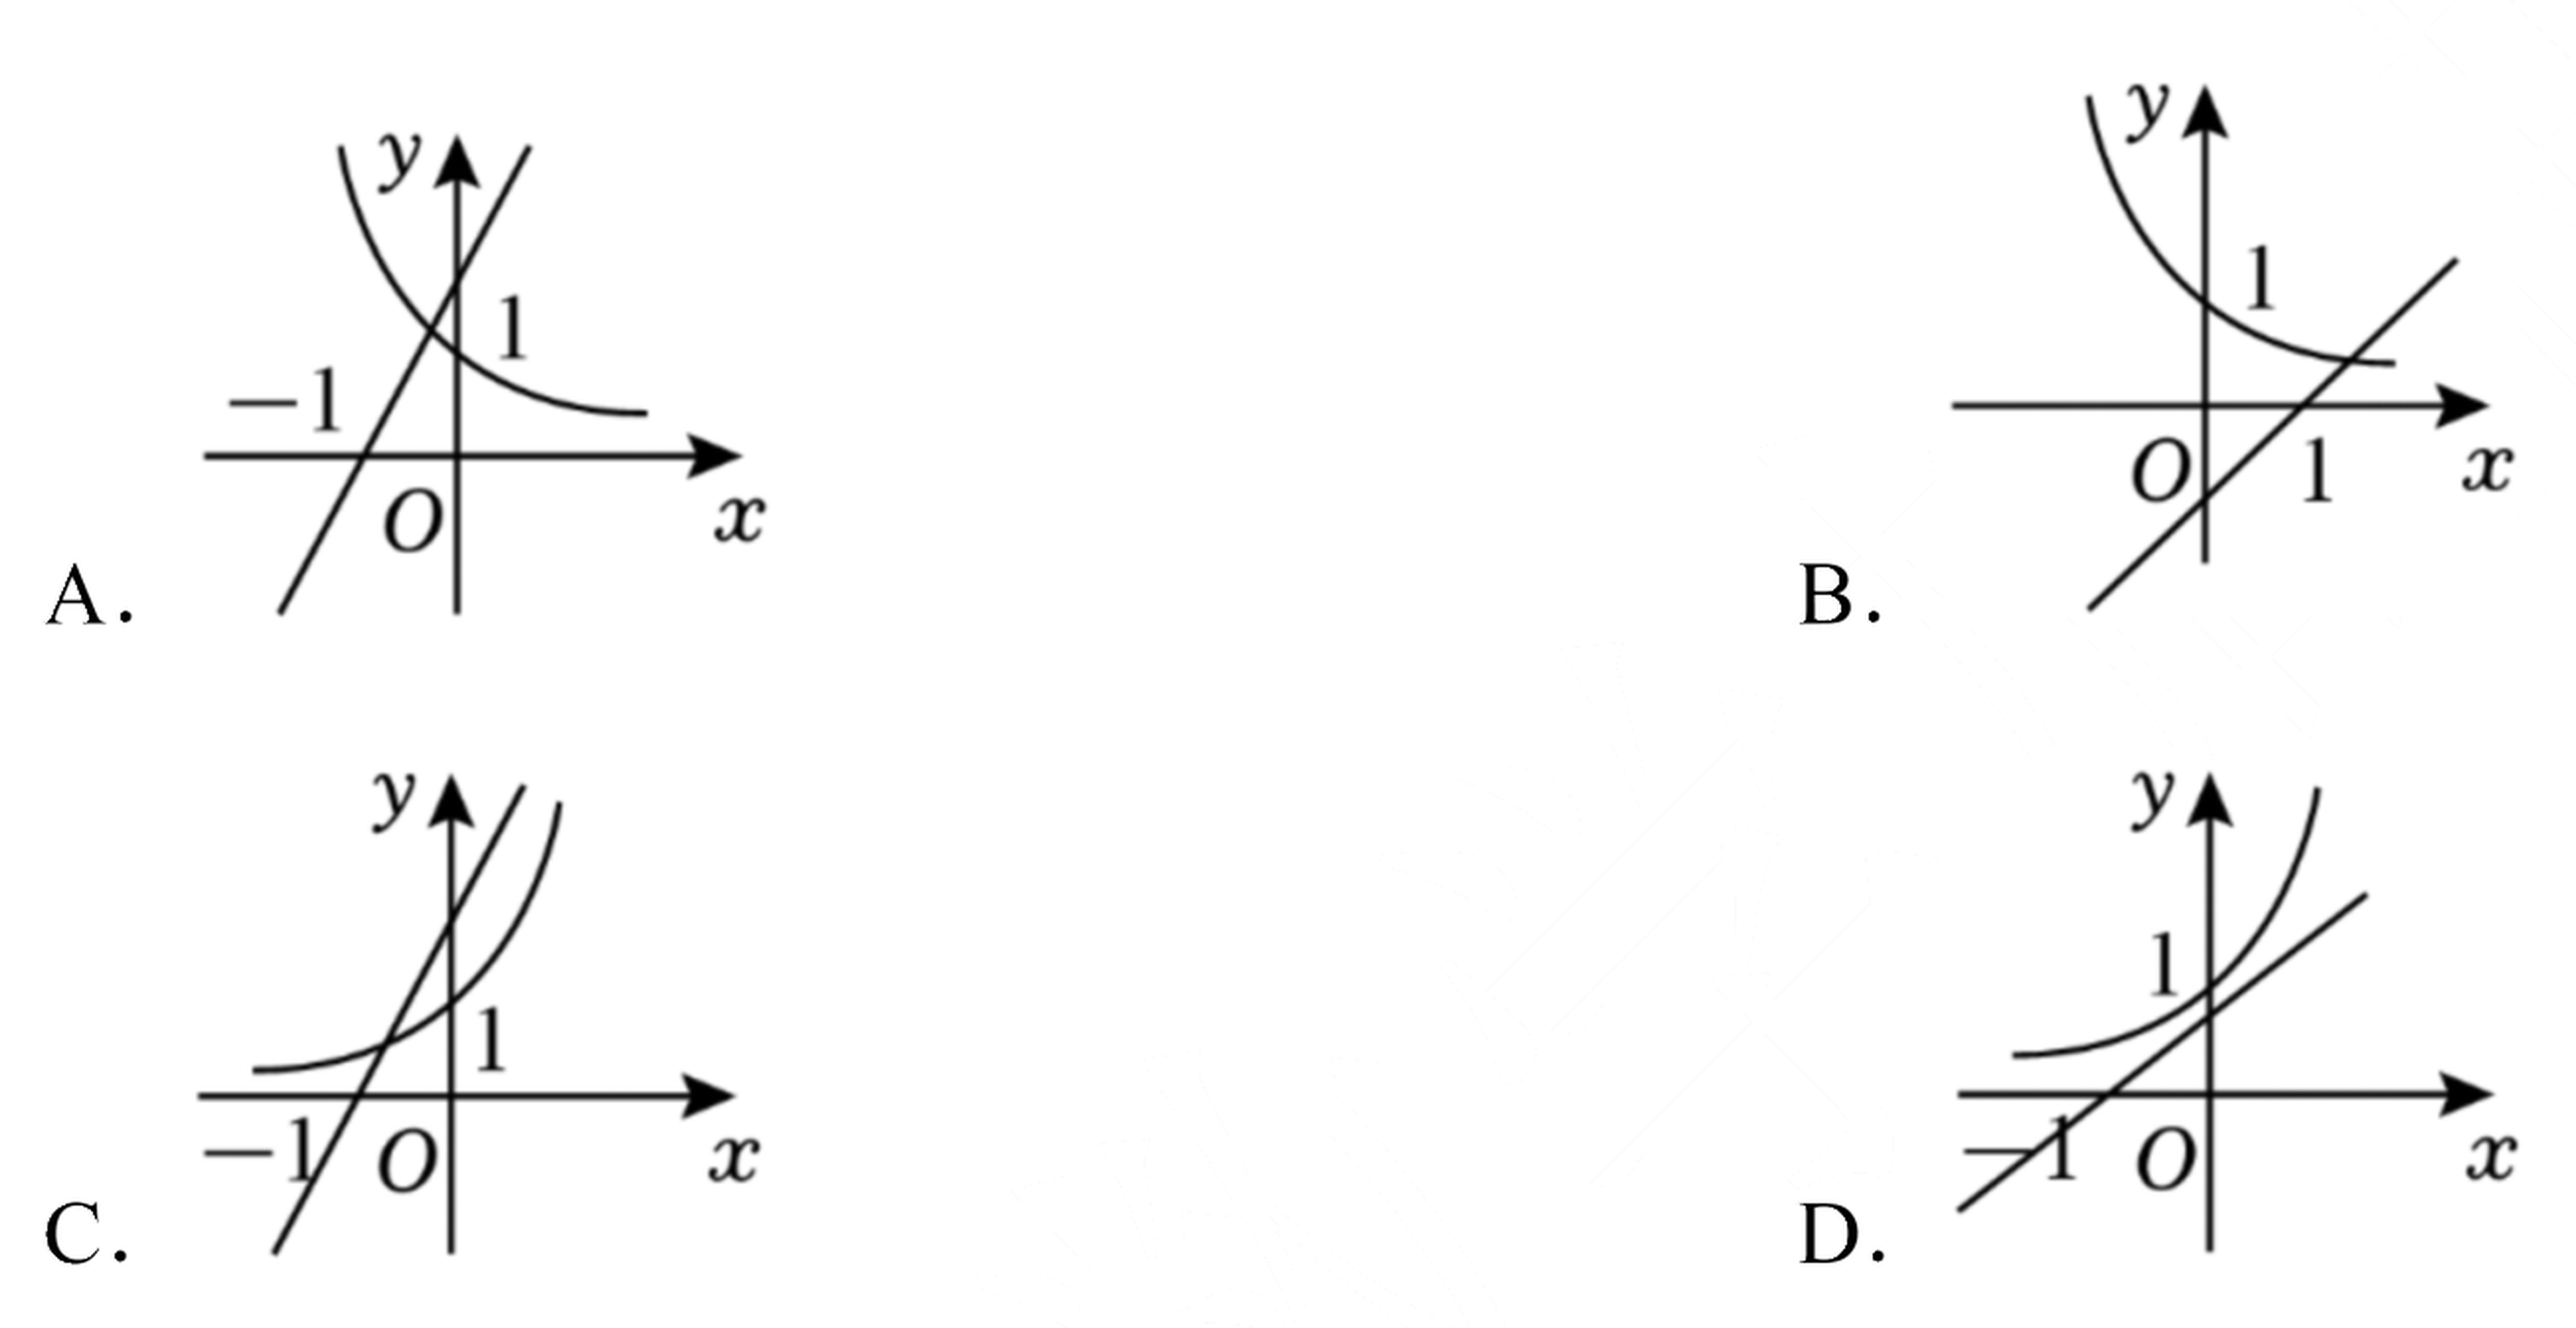
\includegraphics[width=0.80\textwidth]{figures/gao142_q15.png}
\end{center}

\ifanswer
\solbegin
\step{$A$ 中，由指数函数 $y=a^x(a>0\text{ 且 }a\neq1)$ 图像递减得 $0<a<1$，}
\step{而一次函数 $y=a(x+1)$ 的图像与 $y$ 轴交点纵坐标为 $a>1$，二者矛盾，}
\step{所以 $A$ 错；}
\step{由一次函数 $y=a(x+1)$ 的图像与 $x$ 轴交点横坐标为 $-1$，排除 $B$；}
\step{$C$ 中，由指数函数 $y=a^x(a>0\text{ 且 }a\neq1)$ 图像递减得 $a>1$，}% 原卷"递减得 a>1"自相矛盾（递减应得 0<a<1），照录
\step{而一次函数 $y=a(x+1)$ 的图像与 $y$ 轴交点纵坐标为 $a>1$，二者 $a$ 值吻合，}
\step{所以 $C$ 对；}
\step{$D$ 中，由一次函数 $y=a(x+1)$ 的图像得 $a=1$，与 $a>0$ 且 $a\neq1$ 矛盾，}
\step{所以 $D$ 错.}
\step{故选 $C$.}
\solend
\fi

\item 不等式 $\lvert x+1\rvert+\lvert 2-x\rvert\geqslant a^2-2a$ 恒成立，则 $a$ 的取值范围是\mbox{（\quad）}

\keepwithprev
A. $[-1,3]$\qquad B. $(-\infty,3]\cup[3,+\infty)$\qquad C. $(-\infty,3)$\qquad D. $(3,+\infty)$

\ifanswer
\solbegin
\step{因为 $\lvert x+1\rvert+\lvert 2-x\rvert\geqslant\lvert(x+1)+(2-x)\rvert=3$，}
\step{所以 $\lvert x+1\rvert+\lvert 2-x\rvert$ 的最小值为 3，}
\step{因为 $\lvert x+1\rvert+\lvert 2-x\rvert\geqslant a^2-2a$ 恒成立，所以只需 $a^2-2a\leqslant3$，所以 $-1\leqslant a\leqslant3$，}
\step{所以 $a$ 的取值范围为 $[-1,3]$. 故选 $A$.}
\solend
\fi

\end{enumerate}

\bigsec{三、解答题}

\begin{enumerate}
\setcounter{enumi}{16}

\item 已知集合 $A=\left\{x\mid\dfrac{x-3}{x-1}\leqslant0\right\}$，$B=\{x\mid\lvert x-1\rvert<a\}$.

(1) 若 $a=1$，求 $A\cap B$；

(2) 若 $x\in A$ 是 $x\in B$ 的充分条件，求 $a$ 的取值范围.

\ifanswer
\solbegin
\step{(1) 不等式 $\dfrac{x-3}{x-1}\leqslant0$，等价于 $(x-3)(x-1)\leqslant0$ 且 $x-1\neq0$，解得 $1<x\leqslant3$，}
\step{所以 $A=\{x\mid 1<x\leqslant3\}$，}
\step{当 $a=1$ 时，不等式 $\lvert x-1\rvert<a$ 可化为 $\lvert x-1\rvert<1$，所以 $-1<x-1<1$，}
\step{故 $0<x<2$，所以 $B=\{x\mid 0<x<2\}$，}
\step{所以 $A\cap B=\{x\mid 1<x<2\}$；}
\step{(2) 因为 $x\in A$ 是 $x\in B$ 的充分条件，所以 $A\subseteq B$，}% 子集符号原卷印带下划线 $\subseteq$，照录
\step{因为 $A=\{x\mid 1<x\leqslant3\}\neq\varnothing$，所以 $B\neq\varnothing$，故 $a>0$，}
\step{由不等式 $\lvert x-1\rvert<a$，解得 $1-a<x<1+a$，}
\step{所以 $B=\{x\mid 1-a<x<1+a\}$，所以 $\begin{cases}1-a\leqslant1\\1+a>3\end{cases}$，解得 $a>2$，}
\step{所以 $a$ 的取值范围为 $(2,+\infty)$.}
\solend
\fi

\item 计算下列式子的值（请务必书写必要的计算步骤）

(1) $27^{\frac13}+\left(\dfrac76\right)^0+\sqrt{(3-\pi)^2}$；

(2) $\lg25+\lg4+7^{\log_7 2}-\log_2 3\times\log_3 4+\log_3 9$.

\ifanswer
\solbegin
\step{(1) $27^{\frac13}+\left(\dfrac76\right)^0+\sqrt{(3-\pi)^2}=3^{3\times\frac13}+1+\lvert 3-\pi\rvert=3+1+\pi-3=\pi+1$；}
\step{(2) 原式 $=\lg(25\times4)+2-\dfrac{\lg3}{\lg2}\times\dfrac{\lg4}{\lg3}+2=\lg100+2-\dfrac{2\lg2}{\lg2}+2$}
\step{$=2+2-2+2=4$.}
\solend
\fi

\item 已知关于 $x$ 的不等式 $mx^2-(3m^2-m+2)x+6m-2\geqslant0$.

(1) 当 $m=2$ 时，求关于 $x$ 的不等式的解集；

(2) 当 $m>0$ 时，求关于 $x$ 的不等式的解集.

\ifanswer
\solbegin
\step{(1) $m=2$ 时，不等式为 $x^2-6x+5\geqslant0$，即 $(x-1)(x-5)\geqslant0$，}
\step{解得 $x\leqslant1$ 或 $x\geqslant5$，所以不等式的解集是 $\{x\mid x\leqslant1$ 或 $x\geqslant5\}$.}
\step{(2) $m>0$ 时，不等式可化为 $(mx-2)[x-(3m-1)]\geqslant0$，}
\step{即 $\left(x-\dfrac2m\right)[x-(3m-1)]\geqslant0$，}
\step{若 $m=1$，则不等式为 $(x-2)^2\geqslant0$，解得 $x\in\R$；}
\step{若 $0<m<1$，则 $\dfrac2m>3m-1$，解不等式得 $x\geqslant\dfrac2m$ 或 $x\leqslant3m-1$；}
\step{若 $m>1$，则 $\dfrac2m<3m-1$，解不等式得 $x\geqslant3m-1$ 或 $x\leqslant\dfrac2m$；}
\step{综上，$0<m<1$ 时，不等式的解集是 $\{x\mid x\leqslant3m-1$ 或 $x\geqslant\dfrac2m\}$；}
\step{$m=1$ 时，不等式的解集为 $\R$；}
\step{$m>1$ 时，不等式的解集是 $\{x\mid x\leqslant\dfrac2m$ 或 $x\geqslant3m-1\}$.}
\solend
\fi

\item 如图，某人计划用篱笆围成一个一边靠墙（墙足够长）的矩形菜园. 设菜园的长为 $x$ 米，宽为 $y$ 米.

\begin{center}
% 矩形围栏示意图取原卷 07 页截图去粉色水印、去色、LANCZOS 放大；题目配图，三版都出
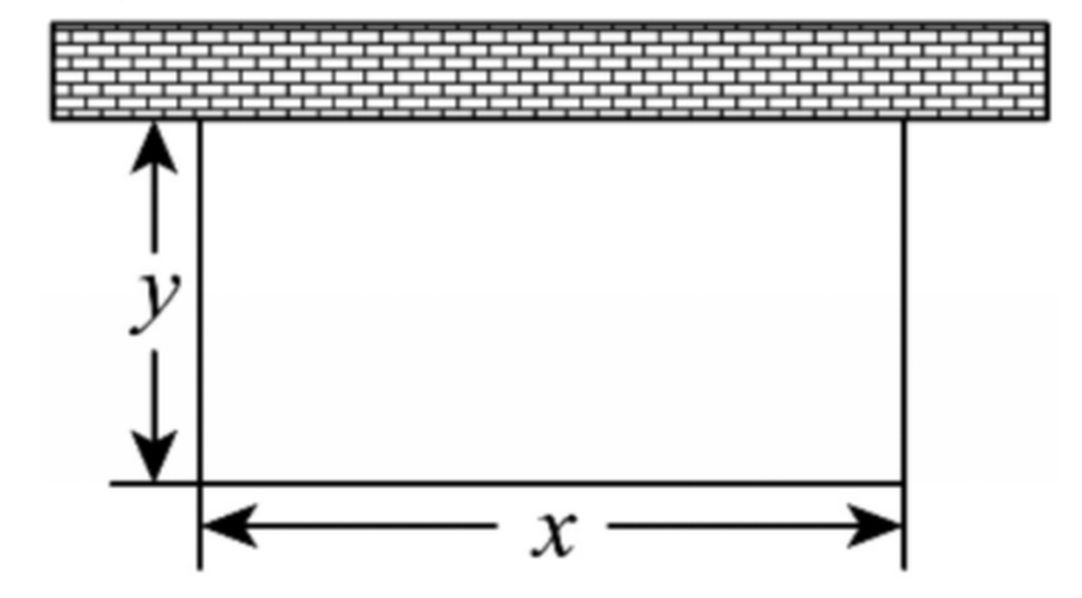
\includegraphics[width=0.42\textwidth]{figures/gao142_q20.png}
\end{center}

(1) 若菜园面积为 72 平方米，则 $x$、$y$ 为何值时，所用篱笆总长最小？

(2) 若 $x$、$y$ 满足 $x+y-xy+63=0$，则菜园面积最小为多少平方米？

\ifanswer
\solbegin
\step{(1) 由题意得，菜园的面积 $S=xy=72$，且 $x>0$，$y>0$，}
\step{所用篱笆总长 $L=x+2y$，}
\step{由基本不等式得 $x+2y\geqslant2\sqrt{x\cdot2y}=2\sqrt{2xy}=2\sqrt{2\times72}=24$，}
\step{当且仅当 $x=2y$ 时取等号，}
\step{联立 $\begin{cases}xy=72\\x=2y\end{cases}$，解得 $\begin{cases}x=12\\y=6\end{cases}$，}
\step{所以当 $x=12$，$y=6$ 时，所用篱笆总长最小；}
\step{(2) 由题意得 $x>0$，$y>0$，且满足 $x+y-xy+63=0$，即 $x+y=xy-63$，}
\step{由基本不等式得 $x+y\geqslant2\sqrt{xy}$，当且仅当 $x=y$ 时取等号，}
\step{所以 $xy-63\geqslant2\sqrt{xy}$. 令 $t=\sqrt{xy}(t>0)$，则 $xy=t^2$，}
\step{上述不等式可化为 $t^2-2t-63\geqslant0$，即 $(t-9)(t+7)\geqslant0$，}
\step{因为 $t>0$，所以 $t+7>0$，故 $t-9\geqslant0$，解得 $t\geqslant9$，所以 $\sqrt{xy}\geqslant9$，}
\step{即 $xy\geqslant81$，当且仅当 $x=y=9$ 时取等号，此时满足 $9+9-81+63=0$，}
\step{所以菜园面积最小为 81 平方米.}
\solend
\fi

\item 已知幂函数 $f(x)=(m^2-3m+3)x^m$ 的图象关于 $y$ 轴对称.

(1) 求实数 $m$ 的值；

(2) 在平面直角坐标系中作出函数 $y=\lvert f(x)-1\rvert$ 的图象；

(3) 已知点 $A(2a,y_1)$ 与点 $B(3-a,y_2)$ 都在幂函数 $y=x^2$ 的图象上. 若 $y_1<y_2$，求实数 $a$ 的取值范围.

\begin{center}
% 空白坐标网格取原卷 08 页截图去粉色水印、去色、LANCZOS 放大；题目配图，三版都出
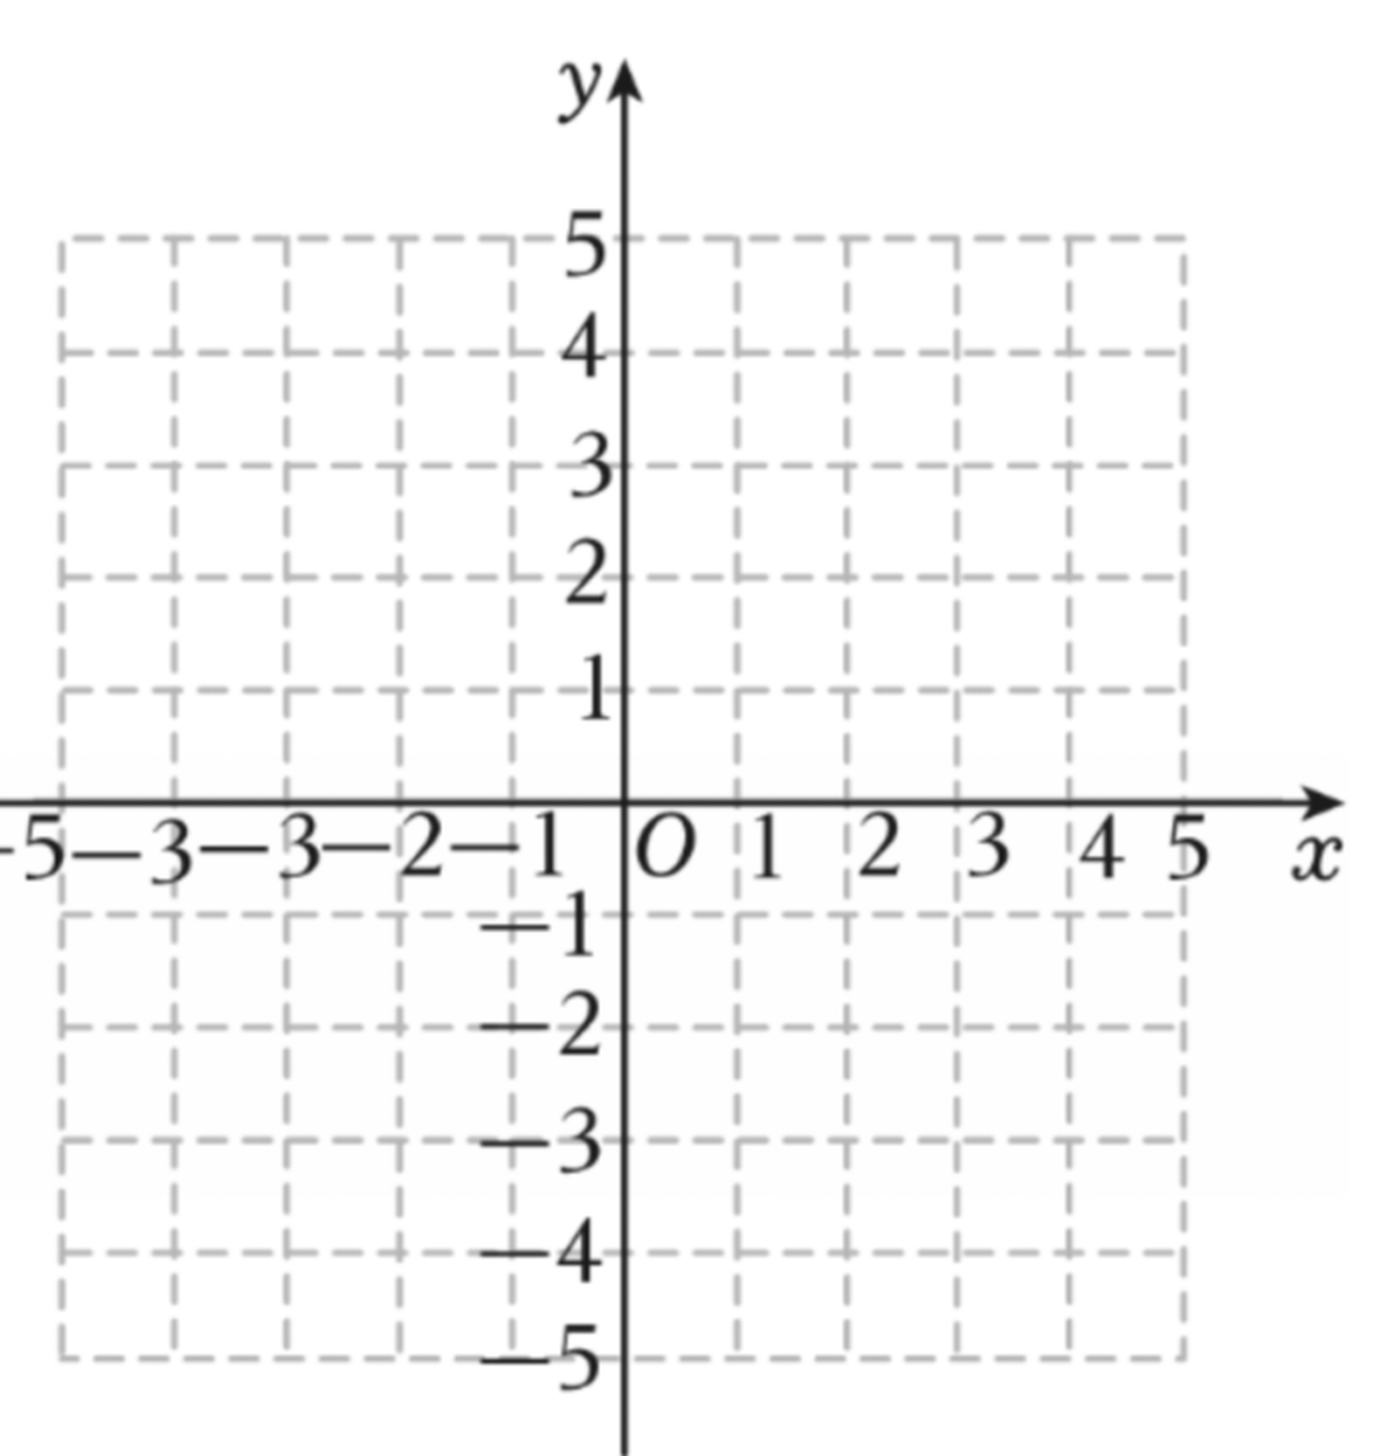
\includegraphics[width=0.52\textwidth]{figures/gao142_q21_grid.png}
\end{center}

\ifanswer
\solbegin
\step{(1) 由题意幂函数 $f(x)=(m^2-3m+3)x^m$，}
\step{故 $m^2-3m+3=1$，解得 $m=1$ 或 $m=2$，}
\step{又 $f(x)$ 图象关于 $y$ 轴对称，即 $f(x)$ 是偶函数，}
\step{当 $m=1$ 时，$f(x)=x$ 是奇函数，不满足条件，舍去；}
\step{当 $m=2$ 时，$f(x)=x^2$ 是偶函数，满足条件，故 $m=2$；}
\step{(2) 由 (1) 得，$\lvert f(x)-1\rvert=\lvert x^2-1\rvert$，}
\step{先画 $y=x^2-1$，开口向上的抛物线，顶点 $(0,-1)$，零点 $x=\pm1$，}
\step{再将 $x$ 轴下方的部分沿 $x$ 轴翻折到上方即为 $y=\lvert x^2-1\rvert$ 的图象，}
\step{图象如图所示.}
\par{\leftskip=0pt
\begin{center}
% 抛物线图象取原卷 09 页截图去粉色水印、去色、LANCZOS 放大；解析所附配图，仅答案版出
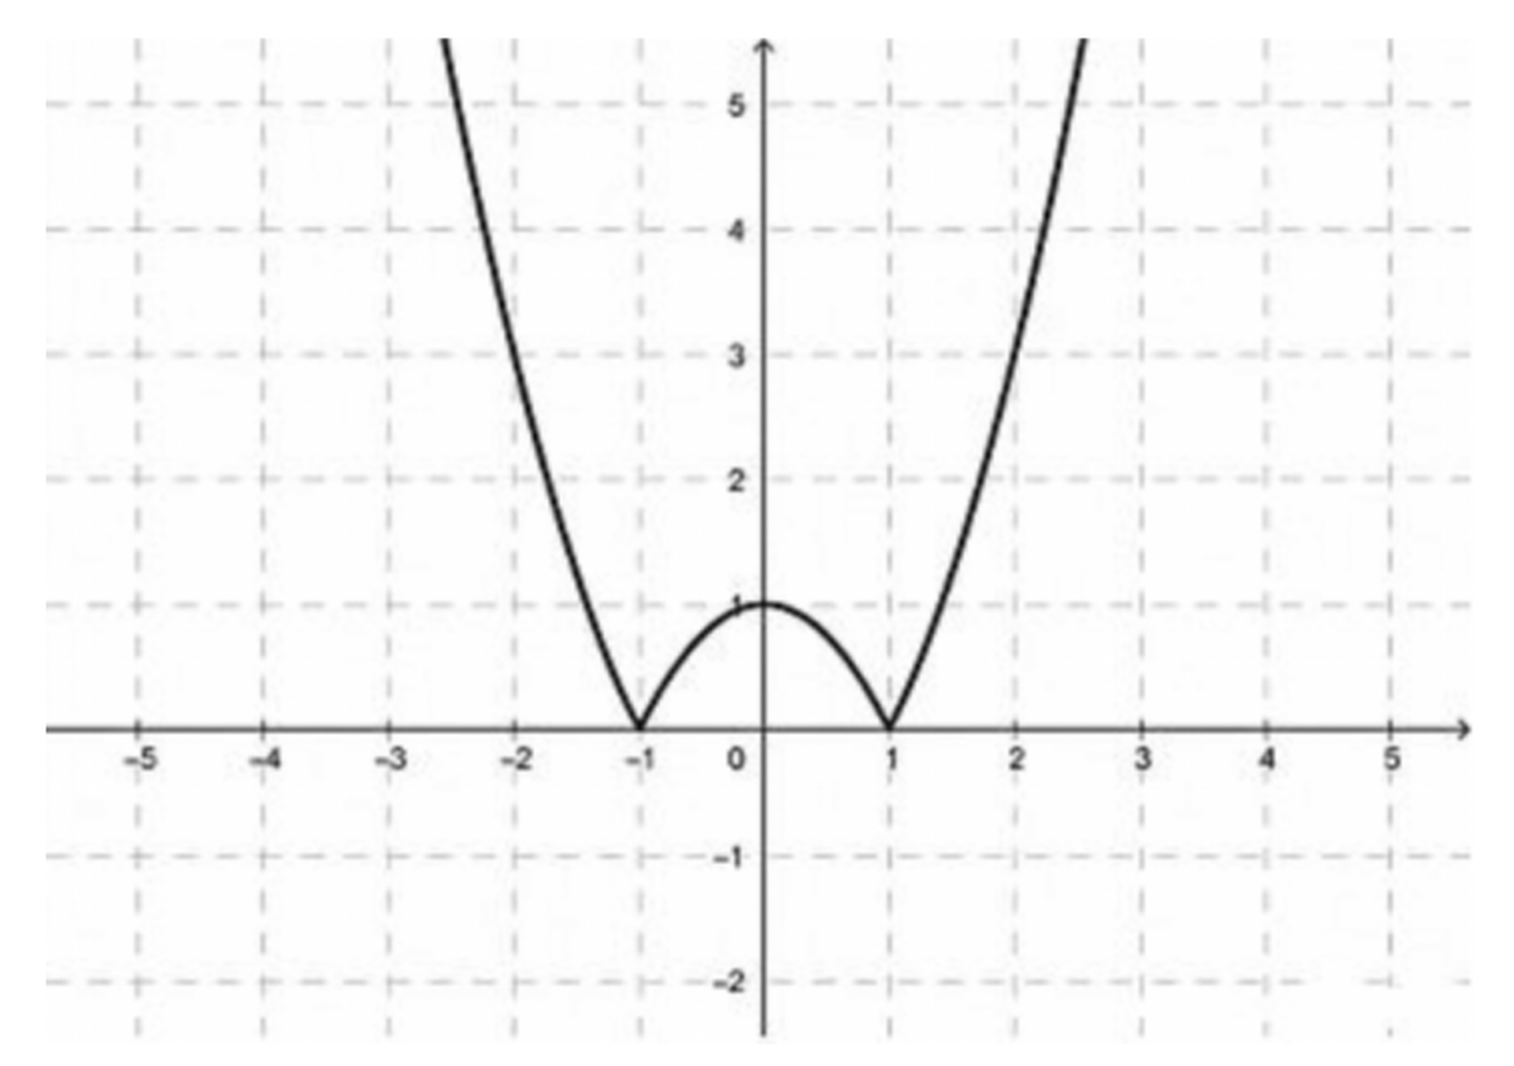
\includegraphics[width=0.55\textwidth]{figures/gao142_q21_para.png}
\end{center}}
\step{(3) 由题意得，$y_1=(2a)^2$，$y_2=(3-a)^2$，}
\step{$y_1<y_2$，即有 $(2a)^2<(3-a)^2$，化简整理得 $(a+3)(a-1)<0$，}
\step{解得实数 $a$ 的取值范围为 $(-3,1)$.}
\solend
\fi

\end{enumerate}

\end{document}
"
%
% ① 原始材料：微信公众号"魔都数学加油站"文章，连载"27学年高一142"，原文标题
% "27学年高一142——2026-2027年上海市群峰高级中学高一上期中"；
% 原文链接：https://mp.weixin.qq.com/s/cc7wnuP4Pk3OjNDV6ihB9A。
% 正文为 9 张 PNG 页（01、02、04、06、07、08、09 为 2560x3620；03、05 为 4762x6735，
% 同一篇各页分辨率不同，逐页按各自分辨率裁图核对），题目下印有【答案】或【解析】，为讲评版。
% 题目、解析均据原图转录；卷面粉红色水印"魔都数学加油站"及公众号页脚未录入。
% 全卷 4 幅插图：第 15 题四幅坐标函数图像选项（04 页，2x2 合并为一张）、
% 第 20 题矩形围栏示意图（07 页）、第 21 题 (2) 空白坐标网格（08 页）、
% 第 21 题抛物线图象（09 页，解析所附图）；均取原卷截图去粉色水印、LANCZOS 放大。
% 题目配图三版都出、解析配图仅答案版出。
%
% 卷首标题：原卷印作"2026-2027 年群峰高级中学高一上期中"（公众号标题中的"上海市"
% 卷面标题行没有，本稿照卷面），年份区间按全稿惯例排 en dash；原卷未印副标题，
% 本卷为期中卷、跨集合与常用逻辑用语／不等式／函数三章，按题目内容补出
% "集合与常用逻辑用语、不等式、函数"（头注说明，与同期中卷口径相同）。
%
% 题号体例：本卷共 19 题——一、填空题 3—12（10 题）、二、选择题 13—16（4 题）、
% 三、解答题 17—21（5 题）。三节分别 \setcounter{enumi}{2}／{12}／{16}。
% 原卷从第 3 题起、无第 1、2 题，本稿保留原题号。
%
% ② 与原卷的排版差异：
%   ① 原文从第 3 题起，本稿保留原题号；原卷未印副标题，本稿按"知识模块"口径补出；
%   ② 逐题答案口径：Q14 原卷把答案 D 印在题干括号内、且题目下无【解析】，本稿括号
%      留空 \mbox{（\quad）}、另提 \ans{D}；Q13／Q15／Q16 答案在【解析】末句"故选 …"
%      （分别为 C／C／A），题干括号留空、不另提 \ans{}；其余各题（Q3—Q12、
%      Q17—Q21）题目下印【解析】、答案融在解析中，不另提 \ans{}；全卷仅 Q14 一处 \ans{}；
%      答案版【答案】/【解析】标记数 = 19（1 个 \ans + 18 个 \solbegin）= 全卷题数；
%   ③ 原卷填空横线按全稿惯例排 \blankline[4.4em]；选择题括号排 \mbox{（\quad）}、
%      每个选项段前按惯例加 \keepwithprev（Q15 四幅图那一枚放在 \begin{center} 之前）；
%      解答题不留作答区、不加 \anspace（原卷为讲评版，与 129／131／132／133／136／140 同）；
%   ④ 原卷数集斜体 $R$（Q5、Q7、Q19、Q21 解析等）按全稿惯例统一改 \R；空集记号
%      \varnothing；绝对值排 \lvert…\rvert，集合描述竖线排 \mid；不等号按全稿惯例
%      排 \leqslant／\geqslant；
%   ⑤ 4 幅插图：Q15 四幅坐标函数图象选项合并裁为一张 \includegraphics（题前
%      \needvspace{9cm}）；Q15 是"二、选择题"节内带大图块的第 3 题（Q13、Q14 在前
%      且无图），另在 \bigsec{二、选择题} 之前加 \needvspace{11cm} 连节标题一起量
%      ——守卫必须放在 \bigsec 之前，放标题之后会让"二、选择题"孤立在页末
%      （B 类，照 高一26／40／59／136／140 成例）；Q20 围栏图与 Q21 网格图置于题干
%      之后（三版都出），Q21 抛物线图置于答案版解析 (2) 与 (3) 之间（仅答案版出）；
%   ⑥ 子题标号按原卷排半角 (1)(2)(3)（与 140／141 同期中卷口径相同）；括注全角／
%      半角逐处照录：Q3"（用含有 m 的代数式表示）"、Q6"（舍）"、Q10"（万元）"、
%      Q18"（请务必书写必要的计算步骤）"、Q20"（墙足够长）"印全角；Q15
%      "$y=a^x(a>0 且 a\neq1)$"、Q10"$y=x^a(a 为常数)$"、Q20"$t=\sqrt{xy}(t>0)$"
%      等数学式内括注印半角；数学式内 CJK 用 \text{…}（否则 FONTCHK 报缺字）；
%   ⑦ 数学式内半角逗号照录（如 Q6"$ax-1=0,a\in\R$"、Q9"$b=2+\sqrt2,a=\sqrt2+1$"、
%      Q16 区间 "$[-1,3]$"、Q21"$y_1<y_2$，即 $(2a)^2<(3-a)^2$" 等）；原卷行末
%      西文句点照录（Q7"(-3,5)."、Q10"125（万元）."、Q19 题干句点、Q20 题干
%      "矩形菜园."与"宽为 y 米."、Q21 题干"对称." 等）；行中全角逗号、分号照录；
%   ⑧ 题干中的中文弯引号：本卷题干与解析通篇未出现中文弯引号，故无此项；
%      圈数字 ①②③ 亦未出现（子题用 (1)(2)(3)）；
%   ⑨ 原卷"图像／图象"两种写法混用，逐处放大核对并照录：Q4 题干与解析作"图象"、
%      Q7 解析作"图象"、Q8 题干作"图像"而解析作"图象"、Q15 题干与解析通篇作
%      "图像"、Q21 题干与解析通篇作"图象"；
%   ⑩ 原卷无红色加粗标签（【解析】均黑色印刷；逐页扫描深红像素为 0），故本卷未用
%      \stepm；黑色常规分步标签（"A 中""C 中""D 中""(1)(2)(3)" 等）按普通 \step
%      行内文字照录；
%   ⑪ 跨页续印按题合并，明细见 ⑥。
%
% ③ 行数复核：一条 \step = 原卷解析的一个印刷行，cases 块作一个印刷行计。逐题数 \step
%   条数，合计 98 条（Q3：1；Q4：2；Q5：3；Q6：4；Q7：5；Q8：2；Q9：4；Q10：3；
%   Q11：4；Q12：3；Q13：5；Q14：0；Q15：10；Q16：4；Q17：10；Q18：3；
%   Q19：10；Q20：13；Q21：12），与原卷印刷行逐题相等。Q14 只把答案印在题干括号、
%   无【解析】，提 \ans{D}、不计入 \step 账；答案版标记数 = 19（1 个 \ans + 18 个
%   \solbegin）= 全卷题数。
%
% ④ 判别式字形：全卷判别式共 3 处——第 7 题【解析】"即判别式△<0"、
%   "即△=(a-1)^2-4×1×4<0" 两处原卷印扁等边三角 $\triangle$，
%   第 11 题【解析】cases 块"△=4a^2-4(a+6)≥0" 一处原卷印等腰偏高的高三角 $\Delta$；
%   逐处放大核对，两形不同、全卷混用，本稿逐处照录不统一（参照 高一141 头注④口径）。
%   子集符号：全卷共 3 处——第 6 题题干"若 B⊆A"、第 6 题【解析】"因为 B⊆A"、
%   第 17 题【解析】(2)"所以 A⊆B"，逐处放大核对，原卷三处均印带下划线的
%   $\subseteq$（不是单线 $\subset$），本稿一律照录 \subseteq；全卷未出现 \subset。
%
% ⑤ 原卷存疑照录（均照录未改，正文对应处另有 % 注）：
%   第 14 题题干括号内原卷印答案 D（非留空），且题目下无【解析】，按"答案印括号且
%      无解析"口径括号留空、另提 \ans{D}；
%   第 15 题【解析】"C 中，由指数函数 … 图像递减得 a>1" 中"递减"与"a>1"
%      自相矛盾（递减应得 0<a<1，疑为"递增"之误），照录；
%   第 16 题选项 B 作 $(-\infty,3]\cup[3,+\infty)$，两端区间并起即全体实数、
%      与正确答案 $[-1,3]$ 不成干扰项（疑为 $(-\infty,-1]\cup[3,+\infty)$ 之误），照录；
%   第 21 题 (2) 空白坐标网格的 x 轴刻度原卷印作"-5 -3 -3 -2 -1 0 1 2 3 4 5"
%      （"-3"重复，疑为"-4"之误），系插图中的印刷内容，取原卷截图照录、不改图。
%
% ⑥ 跨页续印说明：Q7 题干与解析首行在 01 页、解析续至 02 页；Q11 题干与解析
%   4 行在 03 页；Q13 解析前 4 行在 03 页、末句"故选 C."续至 04 页；Q15 题干与
%   四幅图在 04 页、解析前 8 行在 04 页、末 2 行续至 05 页；Q17 解析前 7 行在
%   05 页、后 3 行续至 06 页；Q19 解析前 5 行在 06 页、后 5 行续至 07 页；
%   Q20 解析前 9 行在 07 页、后 4 行续至 08 页；Q21 解析 (1)(2) 9 行在 08 页、
%   抛物线图与 (3) 3 行续至 09 页；本稿按题连排，不丢行。三版切页审计结论见
%   编译自验回报（切页守卫见 ②⑤）。
%
\documentclass[a4paper,11pt]{article}
\usepackage{common}

\begin{document}

\examtitlest[3]{2026--2027 年群峰高级中学高一上期中}{集合与常用逻辑用语、不等式、函数}

\bigsec{一、填空题}

\begin{enumerate}
\setcounter{enumi}{2}

\item 已知 $\log_2 3=m$，则 $\log_3 6=$\blankline[4.4em]（用含有 $m$ 的代数式表示）.

\ifanswer
\solbegin
\step{$\log_3 6=\dfrac{\log_2 6}{\log_2 3}=\dfrac{\log_2 2+\log_2 3}{\log_2 3}=\dfrac{1+m}{m}=\dfrac1m+1$.}
\solend
\fi

\item 若指数函数 $y=a^x$ 的图象经过点 $(3,27)$，则 $a$ 的值为\blankline[4.4em].

\ifanswer
\solbegin
\step{因为指数函数 $y=a^x$ 的图象经过点 $(3,27)$，}
\step{所以 $a^3=27=3^3$，所以 $a=3$.}
\solend
\fi

\item 不等式 $(2x+1)^{\frac13}<(3-x)^{\frac13}$ 的解集为\blankline[4.4em].

\ifanswer
\solbegin
\step{因为幂函数 $f(t)=t^{\frac13}$ 在 $\R$ 上严格增，}
\step{所以原不等式等价于 $2x+1<3-x$，解得 $x<\dfrac23$，}
\step{因此原不等式的解集为 $\left(-\infty,\dfrac23\right)$.}
\solend
\fi

\item 设集合 $A=\{1,-2\}$，$B=\{x\mid ax-1=0,a\in\R\}$，若 $B\subseteq A$，则 $a$ 的值为\blankline[4.4em].% 子集符号原卷印带下划线 $\subseteq$，照录

\ifanswer
\solbegin
\step{因为 $B\subseteq A$，所以 $B=\varnothing$ 或 $\{-2\}$ 或 $\{1\}$ 或 $\{1,-2\}$（舍），}% 子集符号原卷印带下划线 $\subseteq$，照录
\step{若 $B=\varnothing$，则 $a=0$；若 $B=\{1\}$，则 $a=1$；}
\step{若 $B=\{-2\}$，则 $-2a=1$，解得 $a=-\dfrac12$；}
\step{综上，$a=0$ 或 $1$ 或 $-\dfrac12$.}
\solend
\fi

\item 不等式 $x^2+(a-1)x+4>0$ 在 $\R$ 上恒成立，则实数 $a$ 的取值范围是\blankline[4.4em].

\ifanswer
\solbegin
\step{不等式 $x^2+(a-1)x+4>0$，对应的二次函数为 $y=x^2+(a-1)x+4$，}
\step{因此函数图象开口向上，要使不等式对任意实数 $x$ 恒成立，}
\step{需二次函数图象与 $x$ 轴无交点，即判别式 $\triangle<0$，}% 判别式原卷印扁等边三角 $\triangle$，照录
\step{即 $\triangle=(a-1)^2-4\times1\times4<0$，整理得 $a^2-2a-15<0$，}% 判别式原卷印扁等边三角 $\triangle$，照录
\step{解得 $-3<a<5$，故实数 $a$ 的取值范围是 $(-3,5)$.}
\solend
\fi

\item 函数 $f(x)=(5x-3)^a$ 的图像恒过点\blankline[4.4em].% 题干作"图像"、解析作"图象"，原卷混用，逐处照录

\ifanswer
\solbegin
\step{令 $5x-3=1$ 得 $x=\dfrac45$，此时 $f\left(\dfrac45\right)=\left(5\times\dfrac45-3\right)^a=1$，}
\step{所以 $f(x)$ 的图象恒过 $\left(\dfrac45,1\right)$.}
\solend
\fi

\item 若 $a>0$，$b>0$ 且 $\dfrac1a+\dfrac2b=1$，则 $a+b$ 的最小值为\blankline[4.4em].

\ifanswer
\solbegin
\step{因为 $a>0$，$b>0$，$\dfrac1a+\dfrac2b=1$，}
\step{所以 $a+b=(a+b)\left(\dfrac1a+\dfrac2b\right)=1+\dfrac{2a}{b}+\dfrac{b}{a}+2\geqslant3+2\sqrt{\dfrac{2a}{b}\cdot\dfrac{b}{a}}=3+2\sqrt2$，}
\step{当且仅当 $\dfrac{2a}{b}=\dfrac{b}{a}$，即 $b=2+\sqrt2,a=\sqrt2+1$ 时取等号，}
\step{故 $a+b$ 的最小值为 $3+2\sqrt2$.}
\solend
\fi

\item 某药厂研制出一种新型药剂，投放市场后其广告投入 $x$（万元）与药品利润 $y$（万元）存在的关系为 $y=x^a(a\text{ 为常数})$，其中 $x$ 不超过 5 万元. 已知去年投入广告费用为 3 万元时，药品利润为 27 万元，若今年投入广告费用 5 万元，预计今年药品利润为\blankline[4.4em]万元.

\ifanswer
\solbegin
\step{由已知投入广告费用为 3 万元时，药品利润为 27 万元，}
\step{代入 $y=x^a$ 中，即 $3^a=27$，解得 $a=3$，故函数关系式为 $y=x^3$，}
\step{所以当 $x=5$ 时，$y=125$（万元）.}
\solend
\fi

\item 已知方程 $x^2+2ax+a+6=0$ 的两根分别是 $x_1$ 和 $x_2$，且满足 $\dfrac1{x_1}+\dfrac1{x_2}<0$，则实数 $a$ 的取值范围是\blankline[4.4em].

\ifanswer
\solbegin
\step{由于方程 $x^2+2ax+a+6=0$ 的两根分别是 $x_1$ 和 $x_2$，}
\step{则 $\begin{cases}\Delta=4a^2-4(a+6)\geqslant0\\x_1+x_2=-2a\\x_1x_2=a+6\end{cases}$，解得 $a\geqslant3$ 或 $a\leqslant-2$.}% 判别式原卷印等腰偏高的高三角 $\Delta$，照录（与第 7 题扁等边 $\triangle$ 两形混用）
\step{又 $\dfrac1{x_1}+\dfrac1{x_2}<0$，即 $\dfrac{x_1+x_2}{x_1\cdot x_2}<0$，故 $\dfrac{-2a}{a+6}<0$，解得 $a<-6$ 或 $a>0$.}
\step{综上，$a$ 的取值范围是 $(-\infty,-6)\cup[3,+\infty)$.}
\solend
\fi

\item 已知 $b>a>1$，若 $\log_a b-\log_b a=\dfrac32$，$a^b=b^a$，则 $a-b=$\blankline[4.4em].

\ifanswer
\solbegin
\step{因为 $b>a>1$，所以 $\log_a b>1$，}
\step{由 $\log_a b-\log_b a=\log_a b-\dfrac{1}{\log_a b}=\dfrac32$，解得 $\log_a b=2$ 即 $b=a^2$，}
\step{因为 $a^b=b^a=a^{2a}$，所以 $b=2a=a^2$，所以 $a=2$，$b=4$，则 $a-b=-2$.}
\solend
\fi

\end{enumerate}

% 第 15 题四幅图是"二、选择题"节内的大图块；守卫须放在 \bigsec 之前连节标题一起量
\needvspace{11cm}
\bigsec{二、选择题}

\begin{enumerate}
\setcounter{enumi}{12}

\item 若 $a>b$，$c<0$，则下列不等式正确的是\mbox{（\quad）}

\keepwithprev
A. $ab>bc$\qquad B. $a+c<b+c$\qquad C. $ac^2>bc^2$\qquad D. $\dfrac ac>\dfrac bc$

\ifanswer
\solbegin
\step{因为 $a>b$，$c<0$，取 $b=0$，则 $ab=bc=0$，故 $A$ 错误；}
\step{由于 $a>b$，所以 $a+c>b+c$，故 $B$ 错误；}
\step{由 $c<0$ 得 $c^2>0$，所以 $ac^2>bc^2$，故 $C$ 正确；}
\step{由于 $a>b$ 且 $c<0$，所以 $\dfrac ac<\dfrac bc$，故 $D$ 错误.}
\step{故选 $C$.}
\solend
\fi

\item 若 $x>0$，$y>0$，则下列各式中，恒成立的是\mbox{（\quad）}% 原卷题干括号内印答案 D、且题目下无【解析】，本稿括号留空、另提 \ans{D}

\keepwithprev
A. $\lg x+\lg y=\lg(x+y)$\qquad B. $\lg x^2=(\lg x)^2$

C. $\dfrac{\lg x}{\lg y}=\lg(x-y)$\qquad D. $\lg x^{\frac1n}=\dfrac{\lg x}{n}$

\ifanswer
\ans{$D$}
\fi

% 第 15 题四幅坐标函数图象选项是一整块，守卫放在 \item 之前
\needvspace{9cm}
\item 在同一平面直角坐标系中，指数函数 $y=a^x(a>0\text{ 且 }a\neq1)$ 和一次函数 $y=a(x+1)$ 的图像关系可能是\mbox{（\quad）}

\keepwithprev
\begin{center}
% 四幅坐标函数图象选项取原卷 04 页截图去粉色水印、去色，按原卷 2x2 排布合并为一张
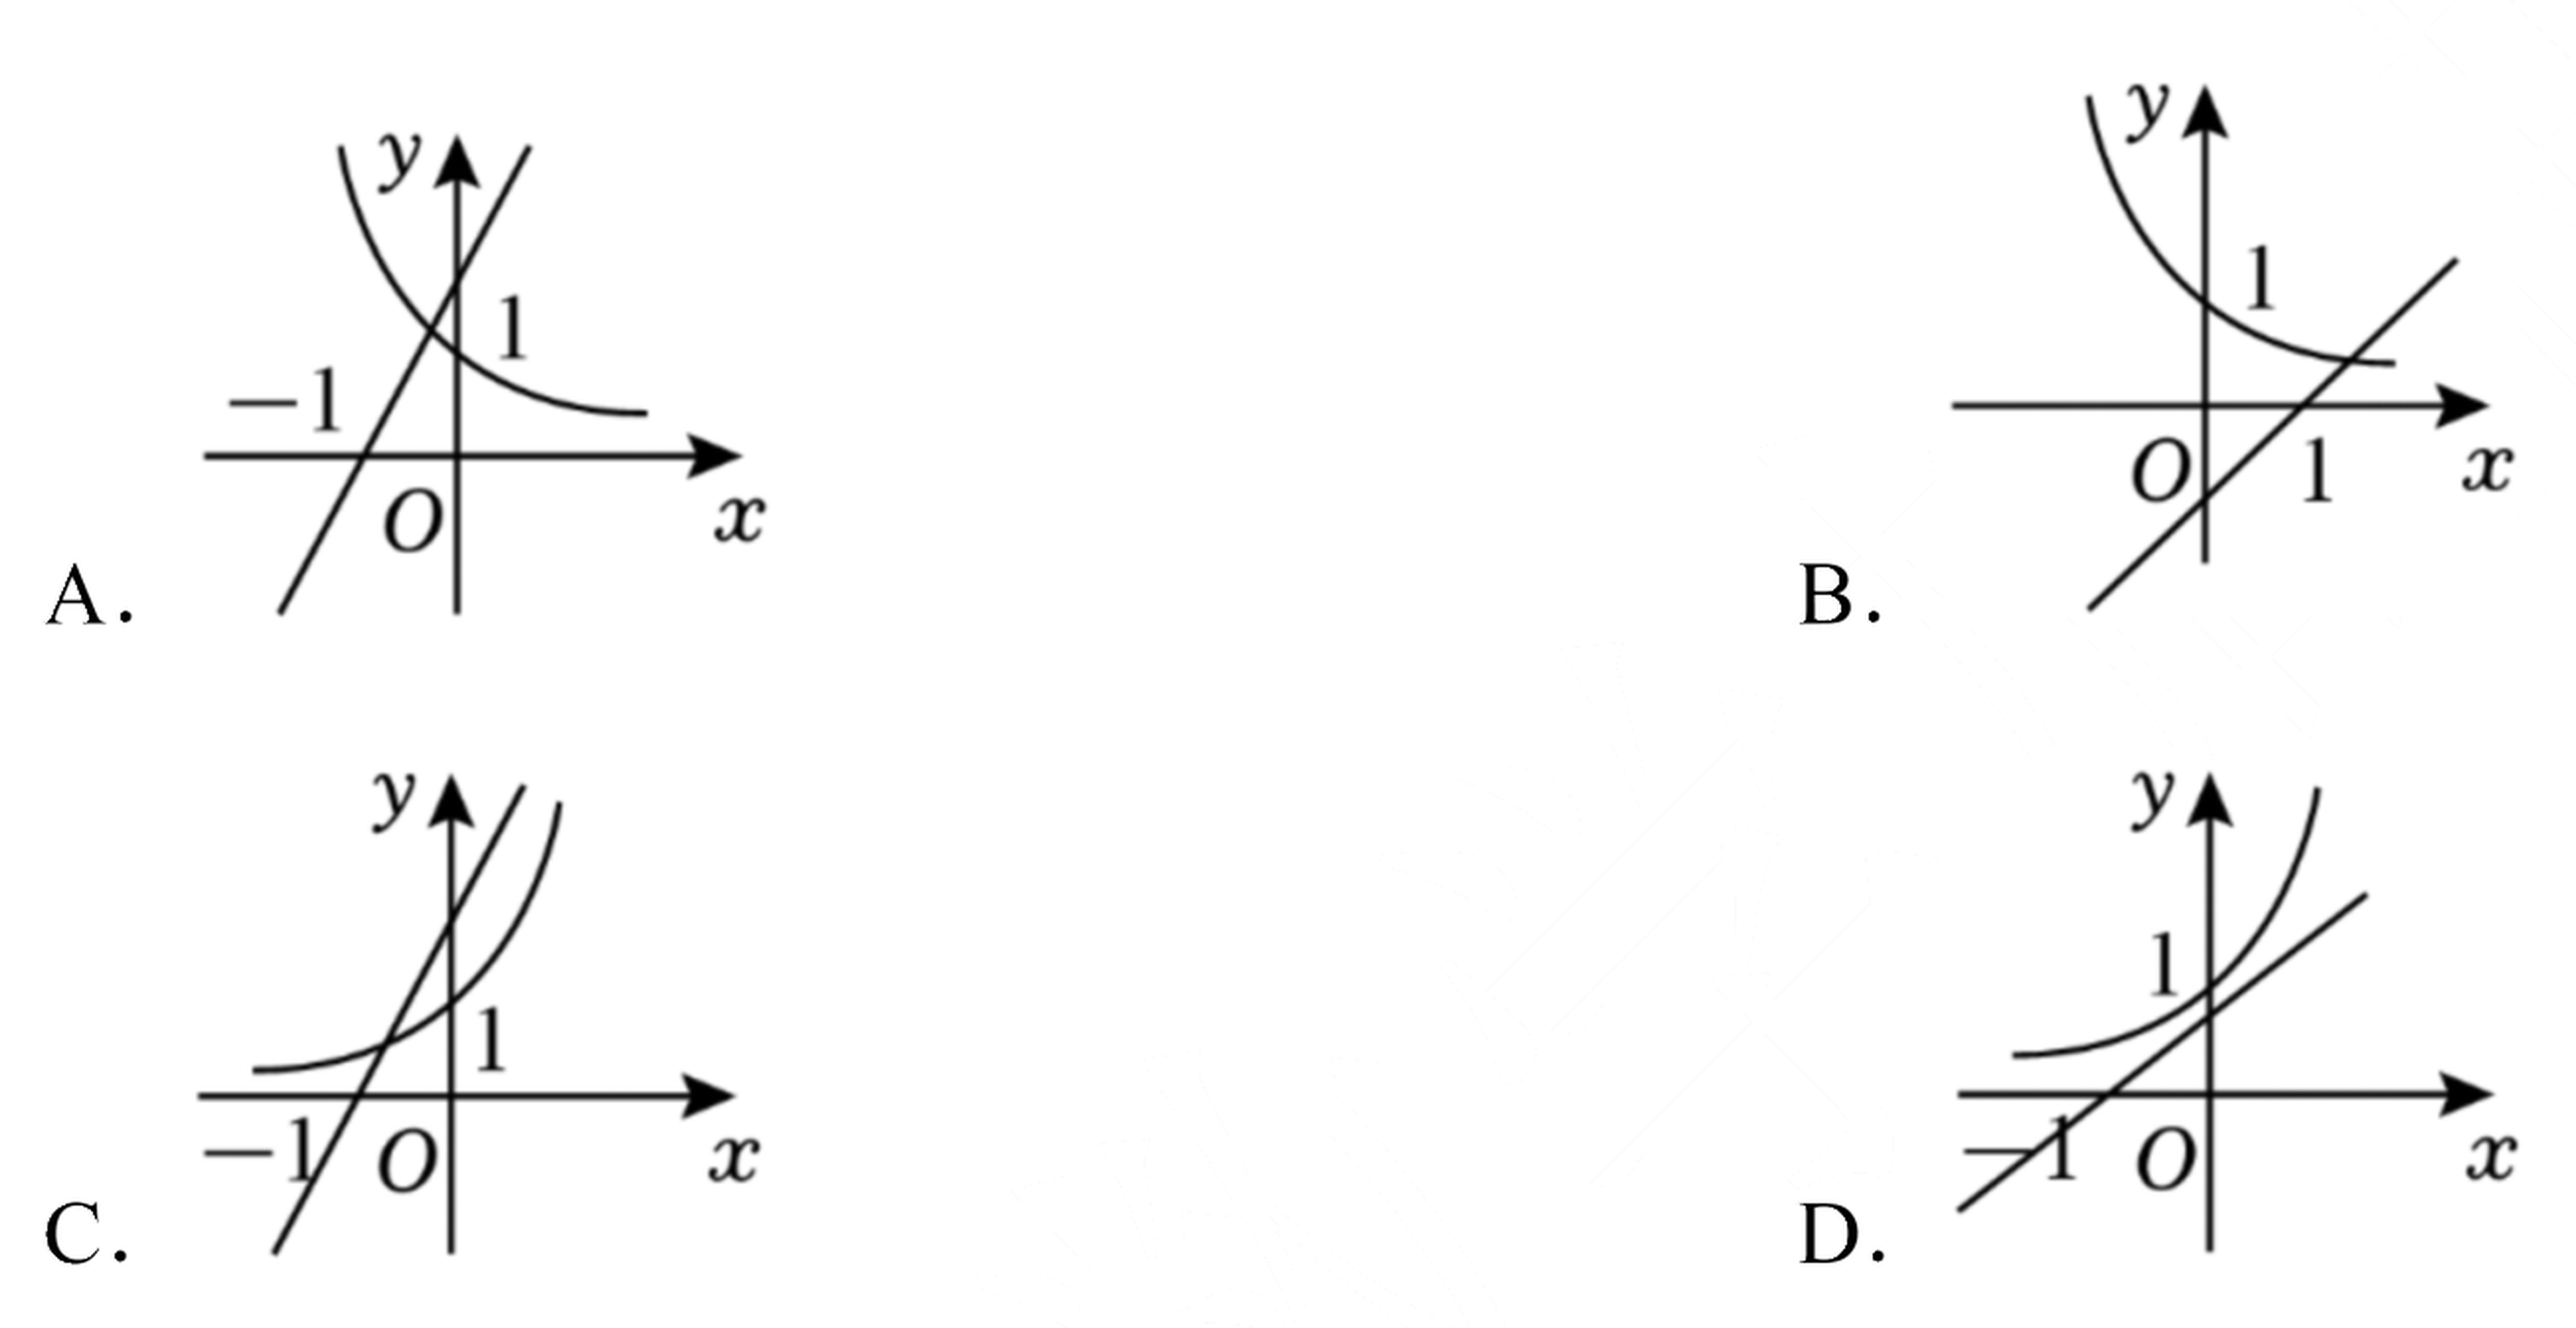
\includegraphics[width=0.80\textwidth]{figures/gao142_q15.png}
\end{center}

\ifanswer
\solbegin
\step{$A$ 中，由指数函数 $y=a^x(a>0\text{ 且 }a\neq1)$ 图像递减得 $0<a<1$，}
\step{而一次函数 $y=a(x+1)$ 的图像与 $y$ 轴交点纵坐标为 $a>1$，二者矛盾，}
\step{所以 $A$ 错；}
\step{由一次函数 $y=a(x+1)$ 的图像与 $x$ 轴交点横坐标为 $-1$，排除 $B$；}
\step{$C$ 中，由指数函数 $y=a^x(a>0\text{ 且 }a\neq1)$ 图像递减得 $a>1$，}% 原卷"递减得 a>1"自相矛盾（递减应得 0<a<1），照录
\step{而一次函数 $y=a(x+1)$ 的图像与 $y$ 轴交点纵坐标为 $a>1$，二者 $a$ 值吻合，}
\step{所以 $C$ 对；}
\step{$D$ 中，由一次函数 $y=a(x+1)$ 的图像得 $a=1$，与 $a>0$ 且 $a\neq1$ 矛盾，}
\step{所以 $D$ 错.}
\step{故选 $C$.}
\solend
\fi

\item 不等式 $\lvert x+1\rvert+\lvert 2-x\rvert\geqslant a^2-2a$ 恒成立，则 $a$ 的取值范围是\mbox{（\quad）}

\keepwithprev
A. $[-1,3]$\qquad B. $(-\infty,3]\cup[3,+\infty)$\qquad C. $(-\infty,3)$\qquad D. $(3,+\infty)$

\ifanswer
\solbegin
\step{因为 $\lvert x+1\rvert+\lvert 2-x\rvert\geqslant\lvert(x+1)+(2-x)\rvert=3$，}
\step{所以 $\lvert x+1\rvert+\lvert 2-x\rvert$ 的最小值为 3，}
\step{因为 $\lvert x+1\rvert+\lvert 2-x\rvert\geqslant a^2-2a$ 恒成立，所以只需 $a^2-2a\leqslant3$，所以 $-1\leqslant a\leqslant3$，}
\step{所以 $a$ 的取值范围为 $[-1,3]$. 故选 $A$.}
\solend
\fi

\end{enumerate}

\bigsec{三、解答题}

\begin{enumerate}
\setcounter{enumi}{16}

\item 已知集合 $A=\left\{x\mid\dfrac{x-3}{x-1}\leqslant0\right\}$，$B=\{x\mid\lvert x-1\rvert<a\}$.

(1) 若 $a=1$，求 $A\cap B$；

(2) 若 $x\in A$ 是 $x\in B$ 的充分条件，求 $a$ 的取值范围.

\ifanswer
\solbegin
\step{(1) 不等式 $\dfrac{x-3}{x-1}\leqslant0$，等价于 $(x-3)(x-1)\leqslant0$ 且 $x-1\neq0$，解得 $1<x\leqslant3$，}
\step{所以 $A=\{x\mid 1<x\leqslant3\}$，}
\step{当 $a=1$ 时，不等式 $\lvert x-1\rvert<a$ 可化为 $\lvert x-1\rvert<1$，所以 $-1<x-1<1$，}
\step{故 $0<x<2$，所以 $B=\{x\mid 0<x<2\}$，}
\step{所以 $A\cap B=\{x\mid 1<x<2\}$；}
\step{(2) 因为 $x\in A$ 是 $x\in B$ 的充分条件，所以 $A\subseteq B$，}% 子集符号原卷印带下划线 $\subseteq$，照录
\step{因为 $A=\{x\mid 1<x\leqslant3\}\neq\varnothing$，所以 $B\neq\varnothing$，故 $a>0$，}
\step{由不等式 $\lvert x-1\rvert<a$，解得 $1-a<x<1+a$，}
\step{所以 $B=\{x\mid 1-a<x<1+a\}$，所以 $\begin{cases}1-a\leqslant1\\1+a>3\end{cases}$，解得 $a>2$，}
\step{所以 $a$ 的取值范围为 $(2,+\infty)$.}
\solend
\fi

\item 计算下列式子的值（请务必书写必要的计算步骤）

(1) $27^{\frac13}+\left(\dfrac76\right)^0+\sqrt{(3-\pi)^2}$；

(2) $\lg25+\lg4+7^{\log_7 2}-\log_2 3\times\log_3 4+\log_3 9$.

\ifanswer
\solbegin
\step{(1) $27^{\frac13}+\left(\dfrac76\right)^0+\sqrt{(3-\pi)^2}=3^{3\times\frac13}+1+\lvert 3-\pi\rvert=3+1+\pi-3=\pi+1$；}
\step{(2) 原式 $=\lg(25\times4)+2-\dfrac{\lg3}{\lg2}\times\dfrac{\lg4}{\lg3}+2=\lg100+2-\dfrac{2\lg2}{\lg2}+2$}
\step{$=2+2-2+2=4$.}
\solend
\fi

\item 已知关于 $x$ 的不等式 $mx^2-(3m^2-m+2)x+6m-2\geqslant0$.

(1) 当 $m=2$ 时，求关于 $x$ 的不等式的解集；

(2) 当 $m>0$ 时，求关于 $x$ 的不等式的解集.

\ifanswer
\solbegin
\step{(1) $m=2$ 时，不等式为 $x^2-6x+5\geqslant0$，即 $(x-1)(x-5)\geqslant0$，}
\step{解得 $x\leqslant1$ 或 $x\geqslant5$，所以不等式的解集是 $\{x\mid x\leqslant1$ 或 $x\geqslant5\}$.}
\step{(2) $m>0$ 时，不等式可化为 $(mx-2)[x-(3m-1)]\geqslant0$，}
\step{即 $\left(x-\dfrac2m\right)[x-(3m-1)]\geqslant0$，}
\step{若 $m=1$，则不等式为 $(x-2)^2\geqslant0$，解得 $x\in\R$；}
\step{若 $0<m<1$，则 $\dfrac2m>3m-1$，解不等式得 $x\geqslant\dfrac2m$ 或 $x\leqslant3m-1$；}
\step{若 $m>1$，则 $\dfrac2m<3m-1$，解不等式得 $x\geqslant3m-1$ 或 $x\leqslant\dfrac2m$；}
\step{综上，$0<m<1$ 时，不等式的解集是 $\{x\mid x\leqslant3m-1$ 或 $x\geqslant\dfrac2m\}$；}
\step{$m=1$ 时，不等式的解集为 $\R$；}
\step{$m>1$ 时，不等式的解集是 $\{x\mid x\leqslant\dfrac2m$ 或 $x\geqslant3m-1\}$.}
\solend
\fi

\item 如图，某人计划用篱笆围成一个一边靠墙（墙足够长）的矩形菜园. 设菜园的长为 $x$ 米，宽为 $y$ 米.

\begin{center}
% 矩形围栏示意图取原卷 07 页截图去粉色水印、去色、LANCZOS 放大；题目配图，三版都出
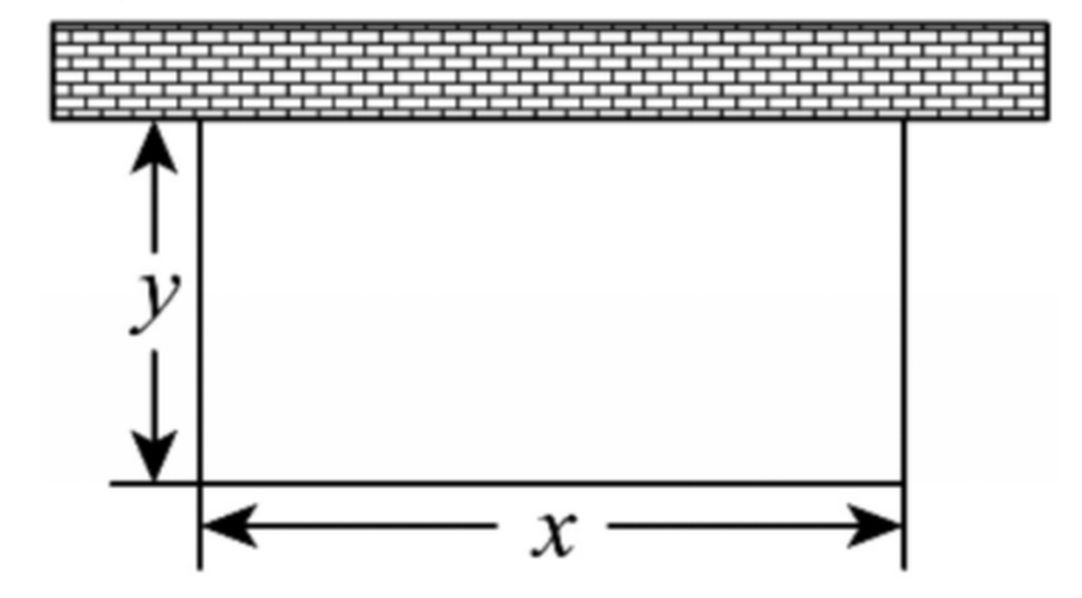
\includegraphics[width=0.42\textwidth]{figures/gao142_q20.png}
\end{center}

(1) 若菜园面积为 72 平方米，则 $x$、$y$ 为何值时，所用篱笆总长最小？

(2) 若 $x$、$y$ 满足 $x+y-xy+63=0$，则菜园面积最小为多少平方米？

\ifanswer
\solbegin
\step{(1) 由题意得，菜园的面积 $S=xy=72$，且 $x>0$，$y>0$，}
\step{所用篱笆总长 $L=x+2y$，}
\step{由基本不等式得 $x+2y\geqslant2\sqrt{x\cdot2y}=2\sqrt{2xy}=2\sqrt{2\times72}=24$，}
\step{当且仅当 $x=2y$ 时取等号，}
\step{联立 $\begin{cases}xy=72\\x=2y\end{cases}$，解得 $\begin{cases}x=12\\y=6\end{cases}$，}
\step{所以当 $x=12$，$y=6$ 时，所用篱笆总长最小；}
\step{(2) 由题意得 $x>0$，$y>0$，且满足 $x+y-xy+63=0$，即 $x+y=xy-63$，}
\step{由基本不等式得 $x+y\geqslant2\sqrt{xy}$，当且仅当 $x=y$ 时取等号，}
\step{所以 $xy-63\geqslant2\sqrt{xy}$. 令 $t=\sqrt{xy}(t>0)$，则 $xy=t^2$，}
\step{上述不等式可化为 $t^2-2t-63\geqslant0$，即 $(t-9)(t+7)\geqslant0$，}
\step{因为 $t>0$，所以 $t+7>0$，故 $t-9\geqslant0$，解得 $t\geqslant9$，所以 $\sqrt{xy}\geqslant9$，}
\step{即 $xy\geqslant81$，当且仅当 $x=y=9$ 时取等号，此时满足 $9+9-81+63=0$，}
\step{所以菜园面积最小为 81 平方米.}
\solend
\fi

\item 已知幂函数 $f(x)=(m^2-3m+3)x^m$ 的图象关于 $y$ 轴对称.

(1) 求实数 $m$ 的值；

(2) 在平面直角坐标系中作出函数 $y=\lvert f(x)-1\rvert$ 的图象；

(3) 已知点 $A(2a,y_1)$ 与点 $B(3-a,y_2)$ 都在幂函数 $y=x^2$ 的图象上. 若 $y_1<y_2$，求实数 $a$ 的取值范围.

\begin{center}
% 空白坐标网格取原卷 08 页截图去粉色水印、去色、LANCZOS 放大；题目配图，三版都出
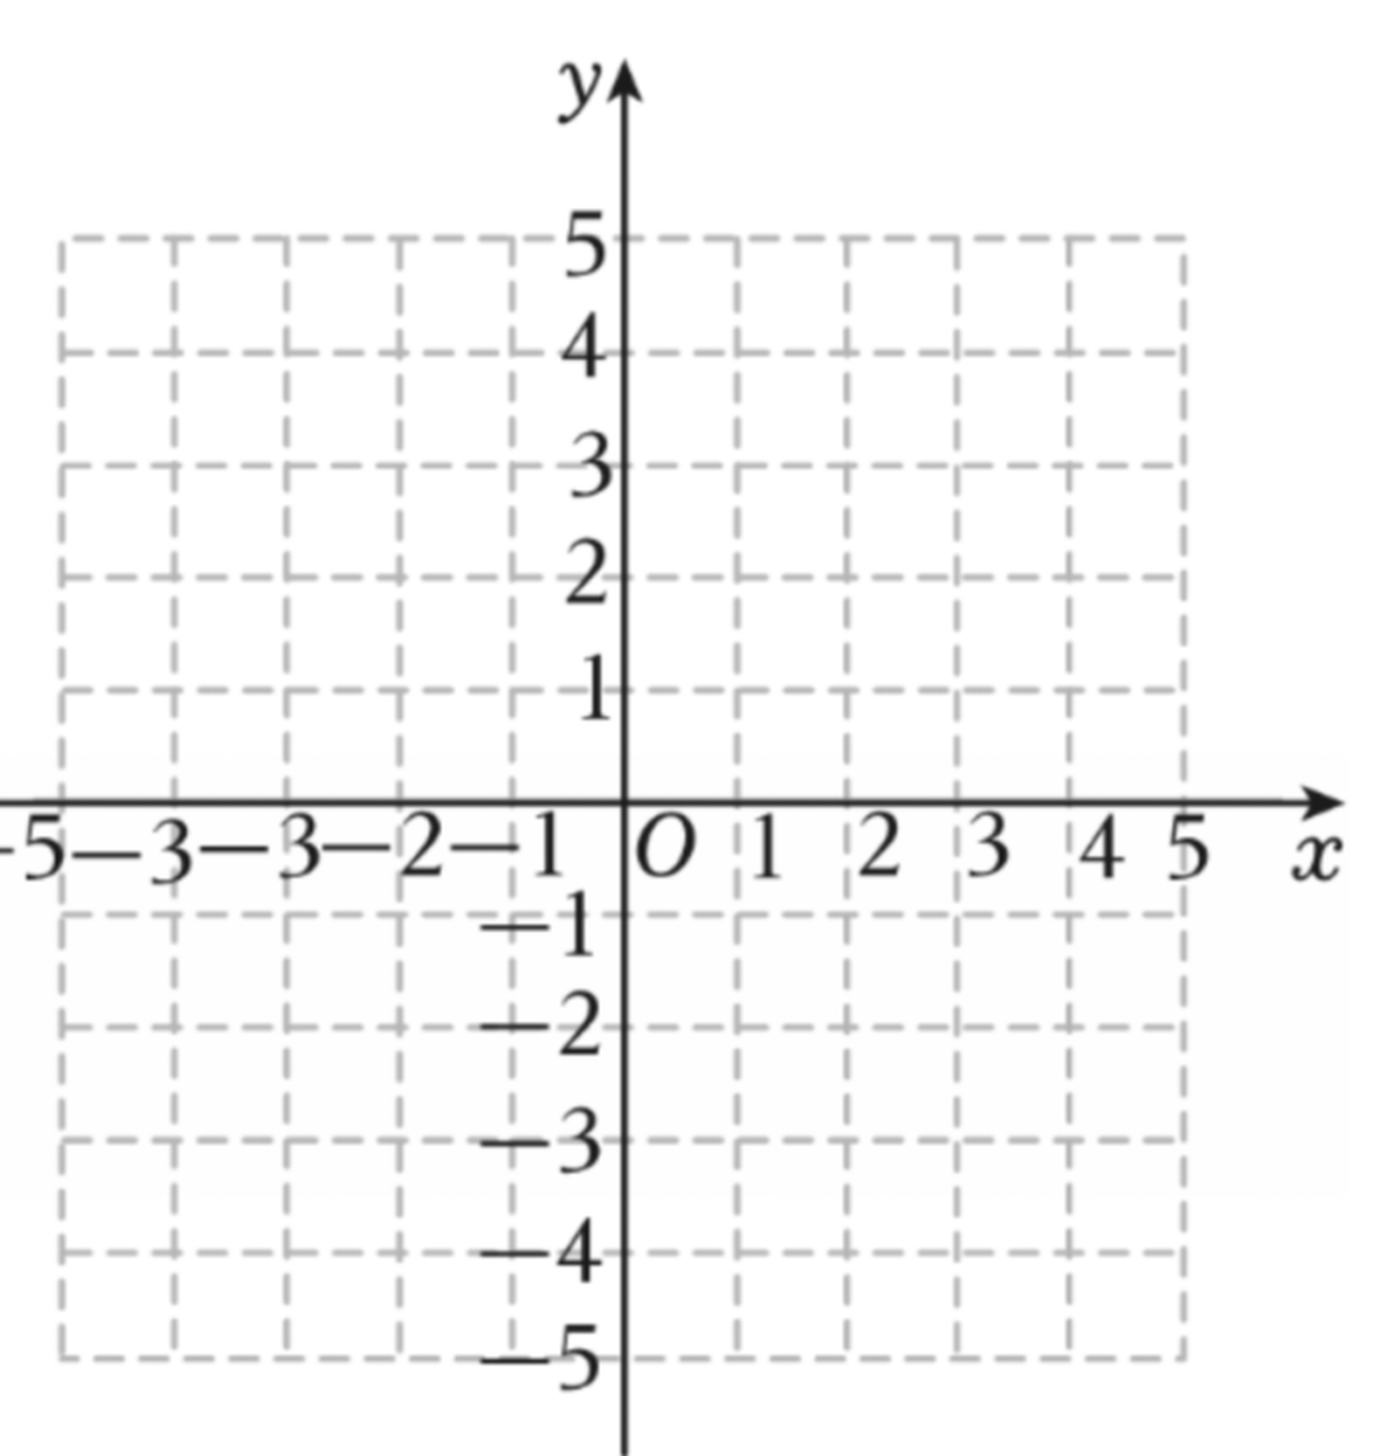
\includegraphics[width=0.52\textwidth]{figures/gao142_q21_grid.png}
\end{center}

\ifanswer
\solbegin
\step{(1) 由题意幂函数 $f(x)=(m^2-3m+3)x^m$，}
\step{故 $m^2-3m+3=1$，解得 $m=1$ 或 $m=2$，}
\step{又 $f(x)$ 图象关于 $y$ 轴对称，即 $f(x)$ 是偶函数，}
\step{当 $m=1$ 时，$f(x)=x$ 是奇函数，不满足条件，舍去；}
\step{当 $m=2$ 时，$f(x)=x^2$ 是偶函数，满足条件，故 $m=2$；}
\step{(2) 由 (1) 得，$\lvert f(x)-1\rvert=\lvert x^2-1\rvert$，}
\step{先画 $y=x^2-1$，开口向上的抛物线，顶点 $(0,-1)$，零点 $x=\pm1$，}
\step{再将 $x$ 轴下方的部分沿 $x$ 轴翻折到上方即为 $y=\lvert x^2-1\rvert$ 的图象，}
\step{图象如图所示.}
\par{\leftskip=0pt
\begin{center}
% 抛物线图象取原卷 09 页截图去粉色水印、去色、LANCZOS 放大；解析所附配图，仅答案版出
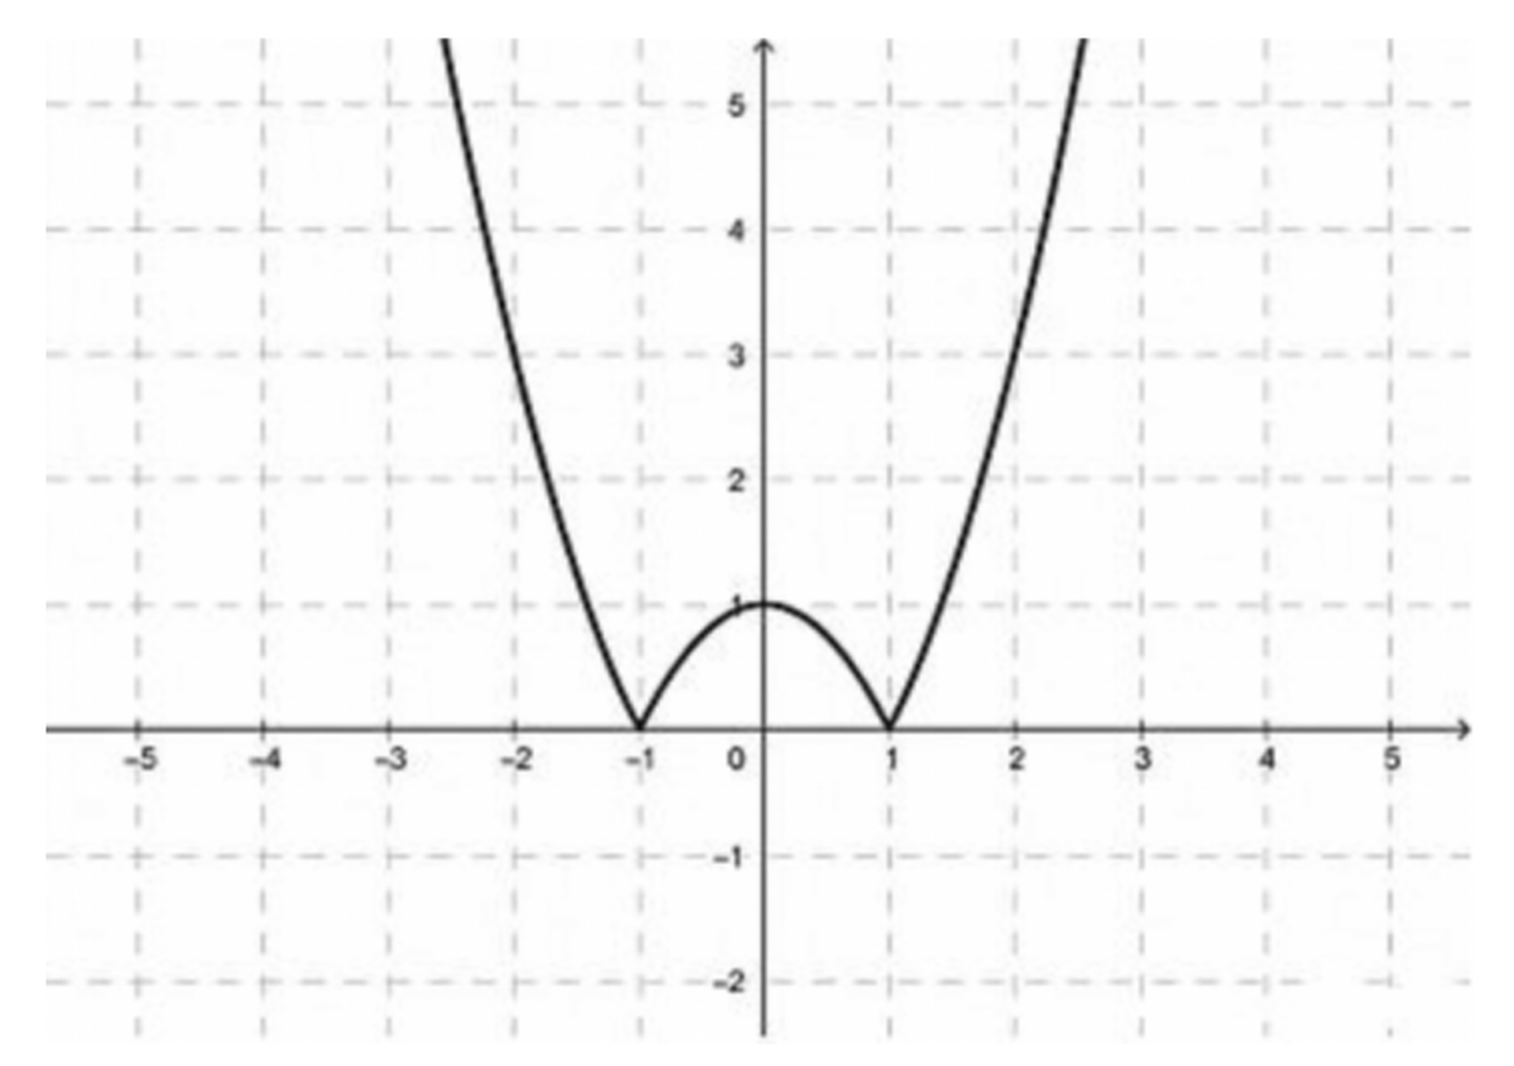
\includegraphics[width=0.55\textwidth]{figures/gao142_q21_para.png}
\end{center}}
\step{(3) 由题意得，$y_1=(2a)^2$，$y_2=(3-a)^2$，}
\step{$y_1<y_2$，即有 $(2a)^2<(3-a)^2$，化简整理得 $(a+3)(a-1)<0$，}
\step{解得实数 $a$ 的取值范围为 $(-3,1)$.}
\solend
\fi

\end{enumerate}

\end{document}
"
%
% ① 原始材料：微信公众号"魔都数学加油站"文章，连载"27学年高一142"，原文标题
% "27学年高一142——2026-2027年上海市群峰高级中学高一上期中"；
% 原文链接：https://mp.weixin.qq.com/s/cc7wnuP4Pk3OjNDV6ihB9A。
% 正文为 9 张 PNG 页（01、02、04、06、07、08、09 为 2560x3620；03、05 为 4762x6735，
% 同一篇各页分辨率不同，逐页按各自分辨率裁图核对），题目下印有【答案】或【解析】，为讲评版。
% 题目、解析均据原图转录；卷面粉红色水印"魔都数学加油站"及公众号页脚未录入。
% 全卷 4 幅插图：第 15 题四幅坐标函数图像选项（04 页，2x2 合并为一张）、
% 第 20 题矩形围栏示意图（07 页）、第 21 题 (2) 空白坐标网格（08 页）、
% 第 21 题抛物线图象（09 页，解析所附图）；均取原卷截图去粉色水印、LANCZOS 放大。
% 题目配图三版都出、解析配图仅答案版出。
%
% 卷首标题：原卷印作"2026-2027 年群峰高级中学高一上期中"（公众号标题中的"上海市"
% 卷面标题行没有，本稿照卷面），年份区间按全稿惯例排 en dash；原卷未印副标题，
% 本卷为期中卷、跨集合与常用逻辑用语／不等式／函数三章，按题目内容补出
% "集合与常用逻辑用语、不等式、函数"（头注说明，与同期中卷口径相同）。
%
% 题号体例：本卷共 19 题——一、填空题 3—12（10 题）、二、选择题 13—16（4 题）、
% 三、解答题 17—21（5 题）。三节分别 \setcounter{enumi}{2}／{12}／{16}。
% 原卷从第 3 题起、无第 1、2 题，本稿保留原题号。
%
% ② 与原卷的排版差异：
%   ① 原文从第 3 题起，本稿保留原题号；原卷未印副标题，本稿按"知识模块"口径补出；
%   ② 逐题答案口径：Q14 原卷把答案 D 印在题干括号内、且题目下无【解析】，本稿括号
%      留空 \mbox{（\quad）}、另提 \ans{D}；Q13／Q15／Q16 答案在【解析】末句"故选 …"
%      （分别为 C／C／A），题干括号留空、不另提 \ans{}；其余各题（Q3—Q12、
%      Q17—Q21）题目下印【解析】、答案融在解析中，不另提 \ans{}；全卷仅 Q14 一处 \ans{}；
%      答案版【答案】/【解析】标记数 = 19（1 个 \ans + 18 个 \solbegin）= 全卷题数；
%   ③ 原卷填空横线按全稿惯例排 \blankline[4.4em]；选择题括号排 \mbox{（\quad）}、
%      每个选项段前按惯例加 \keepwithprev（Q15 四幅图那一枚放在 \begin{center} 之前）；
%      解答题不留作答区、不加 \anspace（原卷为讲评版，与 129／131／132／133／136／140 同）；
%   ④ 原卷数集斜体 $R$（Q5、Q7、Q19、Q21 解析等）按全稿惯例统一改 \R；空集记号
%      \varnothing；绝对值排 \lvert…\rvert，集合描述竖线排 \mid；不等号按全稿惯例
%      排 \leqslant／\geqslant；
%   ⑤ 4 幅插图：Q15 四幅坐标函数图象选项合并裁为一张 \includegraphics（题前
%      \needvspace{9cm}）；Q15 是"二、选择题"节内带大图块的第 3 题（Q13、Q14 在前
%      且无图），另在 \bigsec{二、选择题} 之前加 \needvspace{11cm} 连节标题一起量
%      ——守卫必须放在 \bigsec 之前，放标题之后会让"二、选择题"孤立在页末
%      （B 类，照 高一26／40／59／136／140 成例）；Q20 围栏图与 Q21 网格图置于题干
%      之后（三版都出），Q21 抛物线图置于答案版解析 (2) 与 (3) 之间（仅答案版出）；
%   ⑥ 子题标号按原卷排半角 (1)(2)(3)（与 140／141 同期中卷口径相同）；括注全角／
%      半角逐处照录：Q3"（用含有 m 的代数式表示）"、Q6"（舍）"、Q10"（万元）"、
%      Q18"（请务必书写必要的计算步骤）"、Q20"（墙足够长）"印全角；Q15
%      "$y=a^x(a>0 且 a\neq1)$"、Q10"$y=x^a(a 为常数)$"、Q20"$t=\sqrt{xy}(t>0)$"
%      等数学式内括注印半角；数学式内 CJK 用 \text{…}（否则 FONTCHK 报缺字）；
%   ⑦ 数学式内半角逗号照录（如 Q6"$ax-1=0,a\in\R$"、Q9"$b=2+\sqrt2,a=\sqrt2+1$"、
%      Q16 区间 "$[-1,3]$"、Q21"$y_1<y_2$，即 $(2a)^2<(3-a)^2$" 等）；原卷行末
%      西文句点照录（Q7"(-3,5)."、Q10"125（万元）."、Q19 题干句点、Q20 题干
%      "矩形菜园."与"宽为 y 米."、Q21 题干"对称." 等）；行中全角逗号、分号照录；
%   ⑧ 题干中的中文弯引号：本卷题干与解析通篇未出现中文弯引号，故无此项；
%      圈数字 ①②③ 亦未出现（子题用 (1)(2)(3)）；
%   ⑨ 原卷"图像／图象"两种写法混用，逐处放大核对并照录：Q4 题干与解析作"图象"、
%      Q7 解析作"图象"、Q8 题干作"图像"而解析作"图象"、Q15 题干与解析通篇作
%      "图像"、Q21 题干与解析通篇作"图象"；
%   ⑩ 原卷无红色加粗标签（【解析】均黑色印刷；逐页扫描深红像素为 0），故本卷未用
%      \stepm；黑色常规分步标签（"A 中""C 中""D 中""(1)(2)(3)" 等）按普通 \step
%      行内文字照录；
%   ⑪ 跨页续印按题合并，明细见 ⑥。
%
% ③ 行数复核：一条 \step = 原卷解析的一个印刷行，cases 块作一个印刷行计。逐题数 \step
%   条数，合计 98 条（Q3：1；Q4：2；Q5：3；Q6：4；Q7：5；Q8：2；Q9：4；Q10：3；
%   Q11：4；Q12：3；Q13：5；Q14：0；Q15：10；Q16：4；Q17：10；Q18：3；
%   Q19：10；Q20：13；Q21：12），与原卷印刷行逐题相等。Q14 只把答案印在题干括号、
%   无【解析】，提 \ans{D}、不计入 \step 账；答案版标记数 = 19（1 个 \ans + 18 个
%   \solbegin）= 全卷题数。
%
% ④ 判别式字形：全卷判别式共 3 处——第 7 题【解析】"即判别式△<0"、
%   "即△=(a-1)^2-4×1×4<0" 两处原卷印扁等边三角 $\triangle$，
%   第 11 题【解析】cases 块"△=4a^2-4(a+6)≥0" 一处原卷印等腰偏高的高三角 $\Delta$；
%   逐处放大核对，两形不同、全卷混用，本稿逐处照录不统一（参照 高一141 头注④口径）。
%   子集符号：全卷共 3 处——第 6 题题干"若 B⊆A"、第 6 题【解析】"因为 B⊆A"、
%   第 17 题【解析】(2)"所以 A⊆B"，逐处放大核对，原卷三处均印带下划线的
%   $\subseteq$（不是单线 $\subset$），本稿一律照录 \subseteq；全卷未出现 \subset。
%
% ⑤ 原卷存疑照录（均照录未改，正文对应处另有 % 注）：
%   第 14 题题干括号内原卷印答案 D（非留空），且题目下无【解析】，按"答案印括号且
%      无解析"口径括号留空、另提 \ans{D}；
%   第 15 题【解析】"C 中，由指数函数 … 图像递减得 a>1" 中"递减"与"a>1"
%      自相矛盾（递减应得 0<a<1，疑为"递增"之误），照录；
%   第 16 题选项 B 作 $(-\infty,3]\cup[3,+\infty)$，两端区间并起即全体实数、
%      与正确答案 $[-1,3]$ 不成干扰项（疑为 $(-\infty,-1]\cup[3,+\infty)$ 之误），照录；
%   第 21 题 (2) 空白坐标网格的 x 轴刻度原卷印作"-5 -3 -3 -2 -1 0 1 2 3 4 5"
%      （"-3"重复，疑为"-4"之误），系插图中的印刷内容，取原卷截图照录、不改图。
%
% ⑥ 跨页续印说明：Q7 题干与解析首行在 01 页、解析续至 02 页；Q11 题干与解析
%   4 行在 03 页；Q13 解析前 4 行在 03 页、末句"故选 C."续至 04 页；Q15 题干与
%   四幅图在 04 页、解析前 8 行在 04 页、末 2 行续至 05 页；Q17 解析前 7 行在
%   05 页、后 3 行续至 06 页；Q19 解析前 5 行在 06 页、后 5 行续至 07 页；
%   Q20 解析前 9 行在 07 页、后 4 行续至 08 页；Q21 解析 (1)(2) 9 行在 08 页、
%   抛物线图与 (3) 3 行续至 09 页；本稿按题连排，不丢行。三版切页审计结论见
%   编译自验回报（切页守卫见 ②⑤）。
%
\documentclass[a4paper,11pt]{article}
\usepackage{common}

\begin{document}

\examtitlest[3]{2026--2027 年群峰高级中学高一上期中}{集合与常用逻辑用语、不等式、函数}

\bigsec{一、填空题}

\begin{enumerate}
\setcounter{enumi}{2}

\item 已知 $\log_2 3=m$，则 $\log_3 6=$\blankline[4.4em]（用含有 $m$ 的代数式表示）.

\ifanswer
\solbegin
\step{$\log_3 6=\dfrac{\log_2 6}{\log_2 3}=\dfrac{\log_2 2+\log_2 3}{\log_2 3}=\dfrac{1+m}{m}=\dfrac1m+1$.}
\solend
\fi

\item 若指数函数 $y=a^x$ 的图象经过点 $(3,27)$，则 $a$ 的值为\blankline[4.4em].

\ifanswer
\solbegin
\step{因为指数函数 $y=a^x$ 的图象经过点 $(3,27)$，}
\step{所以 $a^3=27=3^3$，所以 $a=3$.}
\solend
\fi

\item 不等式 $(2x+1)^{\frac13}<(3-x)^{\frac13}$ 的解集为\blankline[4.4em].

\ifanswer
\solbegin
\step{因为幂函数 $f(t)=t^{\frac13}$ 在 $\R$ 上严格增，}
\step{所以原不等式等价于 $2x+1<3-x$，解得 $x<\dfrac23$，}
\step{因此原不等式的解集为 $\left(-\infty,\dfrac23\right)$.}
\solend
\fi

\item 设集合 $A=\{1,-2\}$，$B=\{x\mid ax-1=0,a\in\R\}$，若 $B\subseteq A$，则 $a$ 的值为\blankline[4.4em].% 子集符号原卷印带下划线 $\subseteq$，照录

\ifanswer
\solbegin
\step{因为 $B\subseteq A$，所以 $B=\varnothing$ 或 $\{-2\}$ 或 $\{1\}$ 或 $\{1,-2\}$（舍），}% 子集符号原卷印带下划线 $\subseteq$，照录
\step{若 $B=\varnothing$，则 $a=0$；若 $B=\{1\}$，则 $a=1$；}
\step{若 $B=\{-2\}$，则 $-2a=1$，解得 $a=-\dfrac12$；}
\step{综上，$a=0$ 或 $1$ 或 $-\dfrac12$.}
\solend
\fi

\item 不等式 $x^2+(a-1)x+4>0$ 在 $\R$ 上恒成立，则实数 $a$ 的取值范围是\blankline[4.4em].

\ifanswer
\solbegin
\step{不等式 $x^2+(a-1)x+4>0$，对应的二次函数为 $y=x^2+(a-1)x+4$，}
\step{因此函数图象开口向上，要使不等式对任意实数 $x$ 恒成立，}
\step{需二次函数图象与 $x$ 轴无交点，即判别式 $\triangle<0$，}% 判别式原卷印扁等边三角 $\triangle$，照录
\step{即 $\triangle=(a-1)^2-4\times1\times4<0$，整理得 $a^2-2a-15<0$，}% 判别式原卷印扁等边三角 $\triangle$，照录
\step{解得 $-3<a<5$，故实数 $a$ 的取值范围是 $(-3,5)$.}
\solend
\fi

\item 函数 $f(x)=(5x-3)^a$ 的图像恒过点\blankline[4.4em].% 题干作"图像"、解析作"图象"，原卷混用，逐处照录

\ifanswer
\solbegin
\step{令 $5x-3=1$ 得 $x=\dfrac45$，此时 $f\left(\dfrac45\right)=\left(5\times\dfrac45-3\right)^a=1$，}
\step{所以 $f(x)$ 的图象恒过 $\left(\dfrac45,1\right)$.}
\solend
\fi

\item 若 $a>0$，$b>0$ 且 $\dfrac1a+\dfrac2b=1$，则 $a+b$ 的最小值为\blankline[4.4em].

\ifanswer
\solbegin
\step{因为 $a>0$，$b>0$，$\dfrac1a+\dfrac2b=1$，}
\step{所以 $a+b=(a+b)\left(\dfrac1a+\dfrac2b\right)=1+\dfrac{2a}{b}+\dfrac{b}{a}+2\geqslant3+2\sqrt{\dfrac{2a}{b}\cdot\dfrac{b}{a}}=3+2\sqrt2$，}
\step{当且仅当 $\dfrac{2a}{b}=\dfrac{b}{a}$，即 $b=2+\sqrt2,a=\sqrt2+1$ 时取等号，}
\step{故 $a+b$ 的最小值为 $3+2\sqrt2$.}
\solend
\fi

\item 某药厂研制出一种新型药剂，投放市场后其广告投入 $x$（万元）与药品利润 $y$（万元）存在的关系为 $y=x^a(a\text{ 为常数})$，其中 $x$ 不超过 5 万元. 已知去年投入广告费用为 3 万元时，药品利润为 27 万元，若今年投入广告费用 5 万元，预计今年药品利润为\blankline[4.4em]万元.

\ifanswer
\solbegin
\step{由已知投入广告费用为 3 万元时，药品利润为 27 万元，}
\step{代入 $y=x^a$ 中，即 $3^a=27$，解得 $a=3$，故函数关系式为 $y=x^3$，}
\step{所以当 $x=5$ 时，$y=125$（万元）.}
\solend
\fi

\item 已知方程 $x^2+2ax+a+6=0$ 的两根分别是 $x_1$ 和 $x_2$，且满足 $\dfrac1{x_1}+\dfrac1{x_2}<0$，则实数 $a$ 的取值范围是\blankline[4.4em].

\ifanswer
\solbegin
\step{由于方程 $x^2+2ax+a+6=0$ 的两根分别是 $x_1$ 和 $x_2$，}
\step{则 $\begin{cases}\Delta=4a^2-4(a+6)\geqslant0\\x_1+x_2=-2a\\x_1x_2=a+6\end{cases}$，解得 $a\geqslant3$ 或 $a\leqslant-2$.}% 判别式原卷印等腰偏高的高三角 $\Delta$，照录（与第 7 题扁等边 $\triangle$ 两形混用）
\step{又 $\dfrac1{x_1}+\dfrac1{x_2}<0$，即 $\dfrac{x_1+x_2}{x_1\cdot x_2}<0$，故 $\dfrac{-2a}{a+6}<0$，解得 $a<-6$ 或 $a>0$.}
\step{综上，$a$ 的取值范围是 $(-\infty,-6)\cup[3,+\infty)$.}
\solend
\fi

\item 已知 $b>a>1$，若 $\log_a b-\log_b a=\dfrac32$，$a^b=b^a$，则 $a-b=$\blankline[4.4em].

\ifanswer
\solbegin
\step{因为 $b>a>1$，所以 $\log_a b>1$，}
\step{由 $\log_a b-\log_b a=\log_a b-\dfrac{1}{\log_a b}=\dfrac32$，解得 $\log_a b=2$ 即 $b=a^2$，}
\step{因为 $a^b=b^a=a^{2a}$，所以 $b=2a=a^2$，所以 $a=2$，$b=4$，则 $a-b=-2$.}
\solend
\fi

\end{enumerate}

% 第 15 题四幅图是"二、选择题"节内的大图块；守卫须放在 \bigsec 之前连节标题一起量
\needvspace{11cm}
\bigsec{二、选择题}

\begin{enumerate}
\setcounter{enumi}{12}

\item 若 $a>b$，$c<0$，则下列不等式正确的是\mbox{（\quad）}

\keepwithprev
A. $ab>bc$\qquad B. $a+c<b+c$\qquad C. $ac^2>bc^2$\qquad D. $\dfrac ac>\dfrac bc$

\ifanswer
\solbegin
\step{因为 $a>b$，$c<0$，取 $b=0$，则 $ab=bc=0$，故 $A$ 错误；}
\step{由于 $a>b$，所以 $a+c>b+c$，故 $B$ 错误；}
\step{由 $c<0$ 得 $c^2>0$，所以 $ac^2>bc^2$，故 $C$ 正确；}
\step{由于 $a>b$ 且 $c<0$，所以 $\dfrac ac<\dfrac bc$，故 $D$ 错误.}
\step{故选 $C$.}
\solend
\fi

\item 若 $x>0$，$y>0$，则下列各式中，恒成立的是\mbox{（\quad）}% 原卷题干括号内印答案 D、且题目下无【解析】，本稿括号留空、另提 \ans{D}

\keepwithprev
A. $\lg x+\lg y=\lg(x+y)$\qquad B. $\lg x^2=(\lg x)^2$

C. $\dfrac{\lg x}{\lg y}=\lg(x-y)$\qquad D. $\lg x^{\frac1n}=\dfrac{\lg x}{n}$

\ifanswer
\ans{$D$}
\fi

% 第 15 题四幅坐标函数图象选项是一整块，守卫放在 \item 之前
\needvspace{9cm}
\item 在同一平面直角坐标系中，指数函数 $y=a^x(a>0\text{ 且 }a\neq1)$ 和一次函数 $y=a(x+1)$ 的图像关系可能是\mbox{（\quad）}

\keepwithprev
\begin{center}
% 四幅坐标函数图象选项取原卷 04 页截图去粉色水印、去色，按原卷 2x2 排布合并为一张
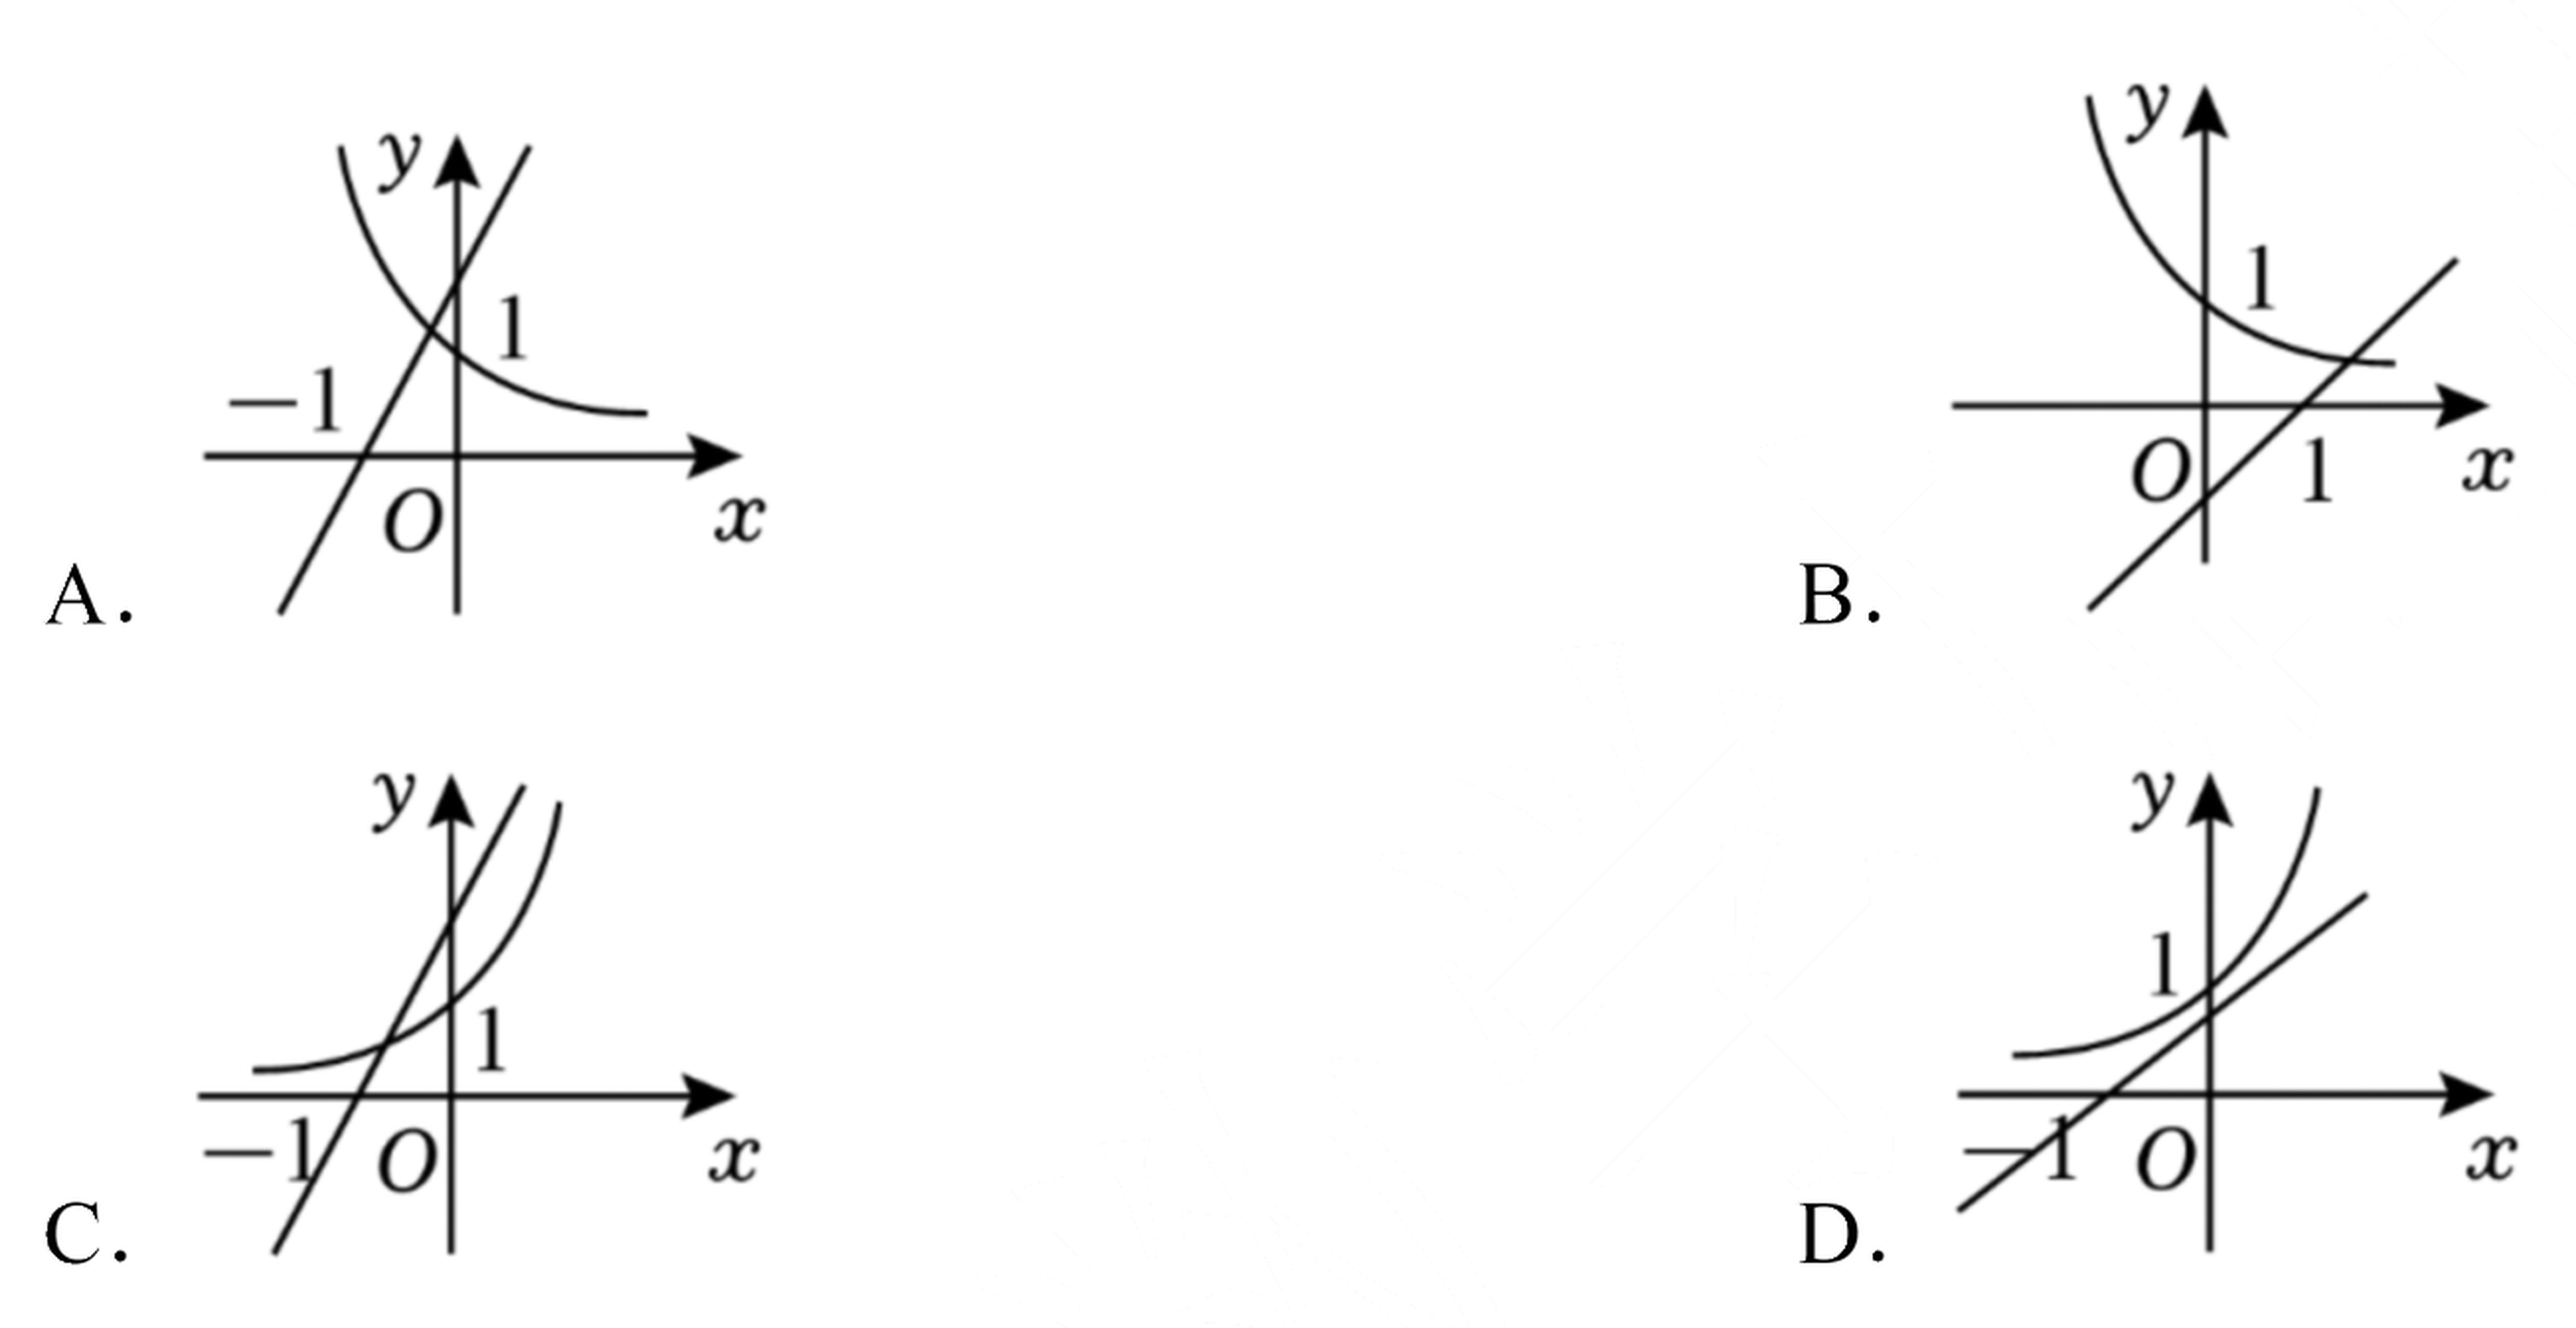
\includegraphics[width=0.80\textwidth]{figures/gao142_q15.png}
\end{center}

\ifanswer
\solbegin
\step{$A$ 中，由指数函数 $y=a^x(a>0\text{ 且 }a\neq1)$ 图像递减得 $0<a<1$，}
\step{而一次函数 $y=a(x+1)$ 的图像与 $y$ 轴交点纵坐标为 $a>1$，二者矛盾，}
\step{所以 $A$ 错；}
\step{由一次函数 $y=a(x+1)$ 的图像与 $x$ 轴交点横坐标为 $-1$，排除 $B$；}
\step{$C$ 中，由指数函数 $y=a^x(a>0\text{ 且 }a\neq1)$ 图像递减得 $a>1$，}% 原卷"递减得 a>1"自相矛盾（递减应得 0<a<1），照录
\step{而一次函数 $y=a(x+1)$ 的图像与 $y$ 轴交点纵坐标为 $a>1$，二者 $a$ 值吻合，}
\step{所以 $C$ 对；}
\step{$D$ 中，由一次函数 $y=a(x+1)$ 的图像得 $a=1$，与 $a>0$ 且 $a\neq1$ 矛盾，}
\step{所以 $D$ 错.}
\step{故选 $C$.}
\solend
\fi

\item 不等式 $\lvert x+1\rvert+\lvert 2-x\rvert\geqslant a^2-2a$ 恒成立，则 $a$ 的取值范围是\mbox{（\quad）}

\keepwithprev
A. $[-1,3]$\qquad B. $(-\infty,3]\cup[3,+\infty)$\qquad C. $(-\infty,3)$\qquad D. $(3,+\infty)$

\ifanswer
\solbegin
\step{因为 $\lvert x+1\rvert+\lvert 2-x\rvert\geqslant\lvert(x+1)+(2-x)\rvert=3$，}
\step{所以 $\lvert x+1\rvert+\lvert 2-x\rvert$ 的最小值为 3，}
\step{因为 $\lvert x+1\rvert+\lvert 2-x\rvert\geqslant a^2-2a$ 恒成立，所以只需 $a^2-2a\leqslant3$，所以 $-1\leqslant a\leqslant3$，}
\step{所以 $a$ 的取值范围为 $[-1,3]$. 故选 $A$.}
\solend
\fi

\end{enumerate}

\bigsec{三、解答题}

\begin{enumerate}
\setcounter{enumi}{16}

\item 已知集合 $A=\left\{x\mid\dfrac{x-3}{x-1}\leqslant0\right\}$，$B=\{x\mid\lvert x-1\rvert<a\}$.

(1) 若 $a=1$，求 $A\cap B$；

(2) 若 $x\in A$ 是 $x\in B$ 的充分条件，求 $a$ 的取值范围.

\ifanswer
\solbegin
\step{(1) 不等式 $\dfrac{x-3}{x-1}\leqslant0$，等价于 $(x-3)(x-1)\leqslant0$ 且 $x-1\neq0$，解得 $1<x\leqslant3$，}
\step{所以 $A=\{x\mid 1<x\leqslant3\}$，}
\step{当 $a=1$ 时，不等式 $\lvert x-1\rvert<a$ 可化为 $\lvert x-1\rvert<1$，所以 $-1<x-1<1$，}
\step{故 $0<x<2$，所以 $B=\{x\mid 0<x<2\}$，}
\step{所以 $A\cap B=\{x\mid 1<x<2\}$；}
\step{(2) 因为 $x\in A$ 是 $x\in B$ 的充分条件，所以 $A\subseteq B$，}% 子集符号原卷印带下划线 $\subseteq$，照录
\step{因为 $A=\{x\mid 1<x\leqslant3\}\neq\varnothing$，所以 $B\neq\varnothing$，故 $a>0$，}
\step{由不等式 $\lvert x-1\rvert<a$，解得 $1-a<x<1+a$，}
\step{所以 $B=\{x\mid 1-a<x<1+a\}$，所以 $\begin{cases}1-a\leqslant1\\1+a>3\end{cases}$，解得 $a>2$，}
\step{所以 $a$ 的取值范围为 $(2,+\infty)$.}
\solend
\fi

\item 计算下列式子的值（请务必书写必要的计算步骤）

(1) $27^{\frac13}+\left(\dfrac76\right)^0+\sqrt{(3-\pi)^2}$；

(2) $\lg25+\lg4+7^{\log_7 2}-\log_2 3\times\log_3 4+\log_3 9$.

\ifanswer
\solbegin
\step{(1) $27^{\frac13}+\left(\dfrac76\right)^0+\sqrt{(3-\pi)^2}=3^{3\times\frac13}+1+\lvert 3-\pi\rvert=3+1+\pi-3=\pi+1$；}
\step{(2) 原式 $=\lg(25\times4)+2-\dfrac{\lg3}{\lg2}\times\dfrac{\lg4}{\lg3}+2=\lg100+2-\dfrac{2\lg2}{\lg2}+2$}
\step{$=2+2-2+2=4$.}
\solend
\fi

\item 已知关于 $x$ 的不等式 $mx^2-(3m^2-m+2)x+6m-2\geqslant0$.

(1) 当 $m=2$ 时，求关于 $x$ 的不等式的解集；

(2) 当 $m>0$ 时，求关于 $x$ 的不等式的解集.

\ifanswer
\solbegin
\step{(1) $m=2$ 时，不等式为 $x^2-6x+5\geqslant0$，即 $(x-1)(x-5)\geqslant0$，}
\step{解得 $x\leqslant1$ 或 $x\geqslant5$，所以不等式的解集是 $\{x\mid x\leqslant1$ 或 $x\geqslant5\}$.}
\step{(2) $m>0$ 时，不等式可化为 $(mx-2)[x-(3m-1)]\geqslant0$，}
\step{即 $\left(x-\dfrac2m\right)[x-(3m-1)]\geqslant0$，}
\step{若 $m=1$，则不等式为 $(x-2)^2\geqslant0$，解得 $x\in\R$；}
\step{若 $0<m<1$，则 $\dfrac2m>3m-1$，解不等式得 $x\geqslant\dfrac2m$ 或 $x\leqslant3m-1$；}
\step{若 $m>1$，则 $\dfrac2m<3m-1$，解不等式得 $x\geqslant3m-1$ 或 $x\leqslant\dfrac2m$；}
\step{综上，$0<m<1$ 时，不等式的解集是 $\{x\mid x\leqslant3m-1$ 或 $x\geqslant\dfrac2m\}$；}
\step{$m=1$ 时，不等式的解集为 $\R$；}
\step{$m>1$ 时，不等式的解集是 $\{x\mid x\leqslant\dfrac2m$ 或 $x\geqslant3m-1\}$.}
\solend
\fi

\item 如图，某人计划用篱笆围成一个一边靠墙（墙足够长）的矩形菜园. 设菜园的长为 $x$ 米，宽为 $y$ 米.

\begin{center}
% 矩形围栏示意图取原卷 07 页截图去粉色水印、去色、LANCZOS 放大；题目配图，三版都出
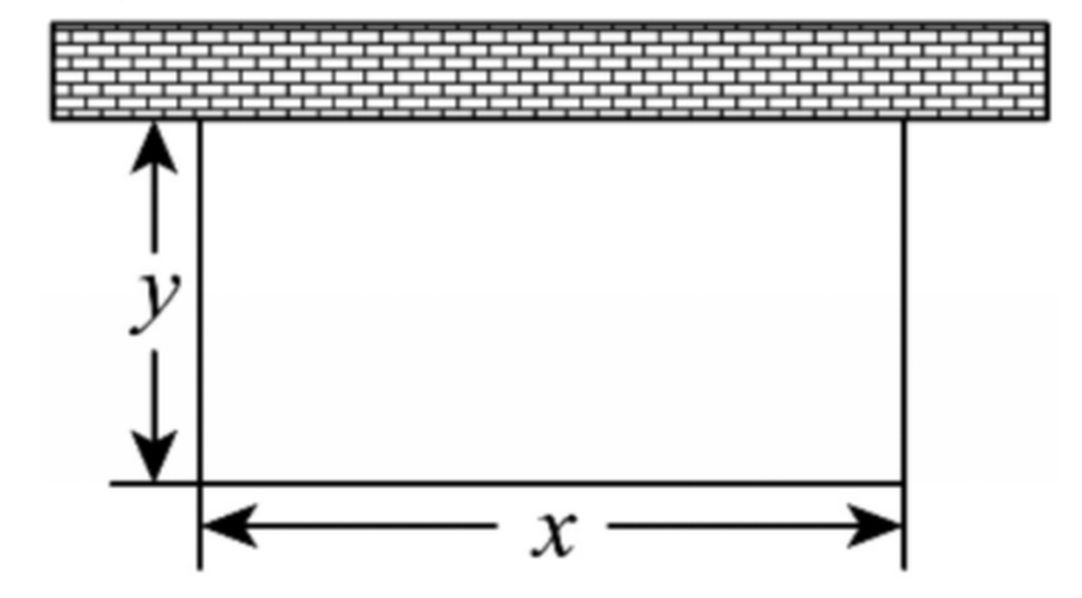
\includegraphics[width=0.42\textwidth]{figures/gao142_q20.png}
\end{center}

(1) 若菜园面积为 72 平方米，则 $x$、$y$ 为何值时，所用篱笆总长最小？

(2) 若 $x$、$y$ 满足 $x+y-xy+63=0$，则菜园面积最小为多少平方米？

\ifanswer
\solbegin
\step{(1) 由题意得，菜园的面积 $S=xy=72$，且 $x>0$，$y>0$，}
\step{所用篱笆总长 $L=x+2y$，}
\step{由基本不等式得 $x+2y\geqslant2\sqrt{x\cdot2y}=2\sqrt{2xy}=2\sqrt{2\times72}=24$，}
\step{当且仅当 $x=2y$ 时取等号，}
\step{联立 $\begin{cases}xy=72\\x=2y\end{cases}$，解得 $\begin{cases}x=12\\y=6\end{cases}$，}
\step{所以当 $x=12$，$y=6$ 时，所用篱笆总长最小；}
\step{(2) 由题意得 $x>0$，$y>0$，且满足 $x+y-xy+63=0$，即 $x+y=xy-63$，}
\step{由基本不等式得 $x+y\geqslant2\sqrt{xy}$，当且仅当 $x=y$ 时取等号，}
\step{所以 $xy-63\geqslant2\sqrt{xy}$. 令 $t=\sqrt{xy}(t>0)$，则 $xy=t^2$，}
\step{上述不等式可化为 $t^2-2t-63\geqslant0$，即 $(t-9)(t+7)\geqslant0$，}
\step{因为 $t>0$，所以 $t+7>0$，故 $t-9\geqslant0$，解得 $t\geqslant9$，所以 $\sqrt{xy}\geqslant9$，}
\step{即 $xy\geqslant81$，当且仅当 $x=y=9$ 时取等号，此时满足 $9+9-81+63=0$，}
\step{所以菜园面积最小为 81 平方米.}
\solend
\fi

\item 已知幂函数 $f(x)=(m^2-3m+3)x^m$ 的图象关于 $y$ 轴对称.

(1) 求实数 $m$ 的值；

(2) 在平面直角坐标系中作出函数 $y=\lvert f(x)-1\rvert$ 的图象；

(3) 已知点 $A(2a,y_1)$ 与点 $B(3-a,y_2)$ 都在幂函数 $y=x^2$ 的图象上. 若 $y_1<y_2$，求实数 $a$ 的取值范围.

\begin{center}
% 空白坐标网格取原卷 08 页截图去粉色水印、去色、LANCZOS 放大；题目配图，三版都出
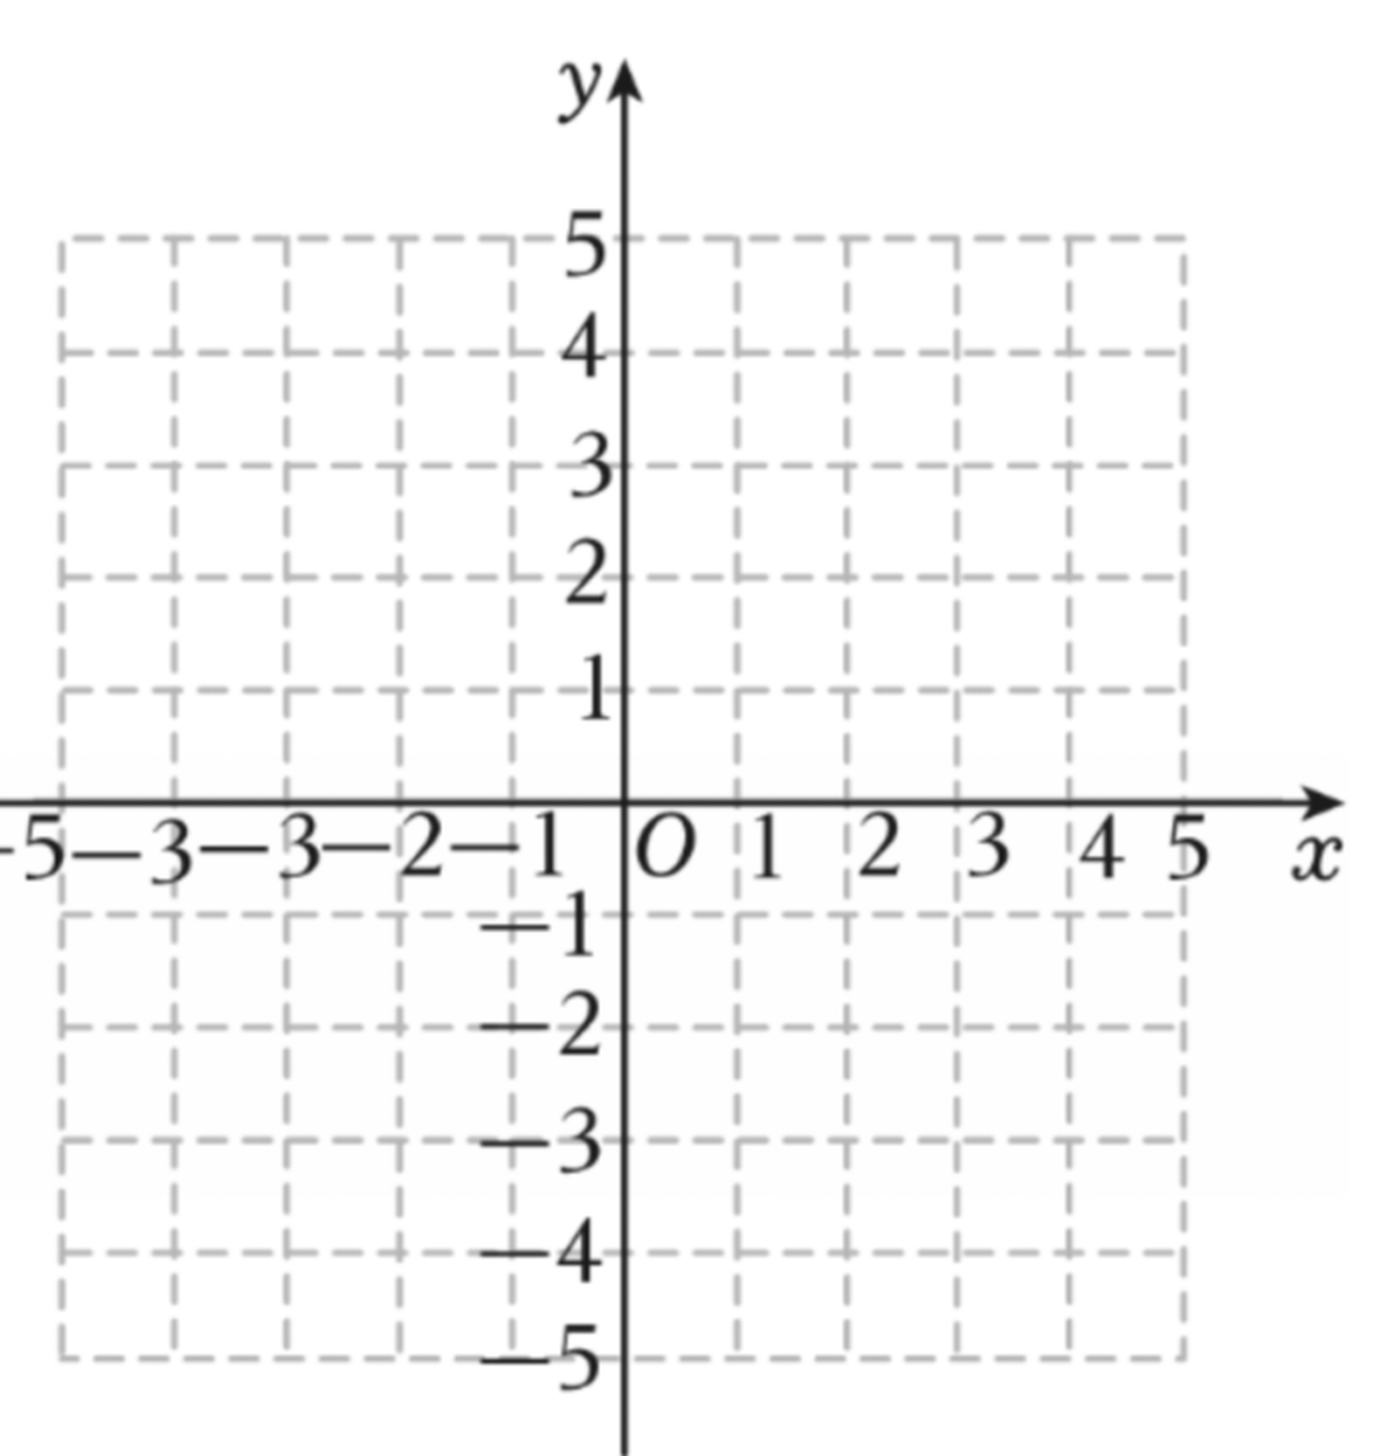
\includegraphics[width=0.52\textwidth]{figures/gao142_q21_grid.png}
\end{center}

\ifanswer
\solbegin
\step{(1) 由题意幂函数 $f(x)=(m^2-3m+3)x^m$，}
\step{故 $m^2-3m+3=1$，解得 $m=1$ 或 $m=2$，}
\step{又 $f(x)$ 图象关于 $y$ 轴对称，即 $f(x)$ 是偶函数，}
\step{当 $m=1$ 时，$f(x)=x$ 是奇函数，不满足条件，舍去；}
\step{当 $m=2$ 时，$f(x)=x^2$ 是偶函数，满足条件，故 $m=2$；}
\step{(2) 由 (1) 得，$\lvert f(x)-1\rvert=\lvert x^2-1\rvert$，}
\step{先画 $y=x^2-1$，开口向上的抛物线，顶点 $(0,-1)$，零点 $x=\pm1$，}
\step{再将 $x$ 轴下方的部分沿 $x$ 轴翻折到上方即为 $y=\lvert x^2-1\rvert$ 的图象，}
\step{图象如图所示.}
\par{\leftskip=0pt
\begin{center}
% 抛物线图象取原卷 09 页截图去粉色水印、去色、LANCZOS 放大；解析所附配图，仅答案版出
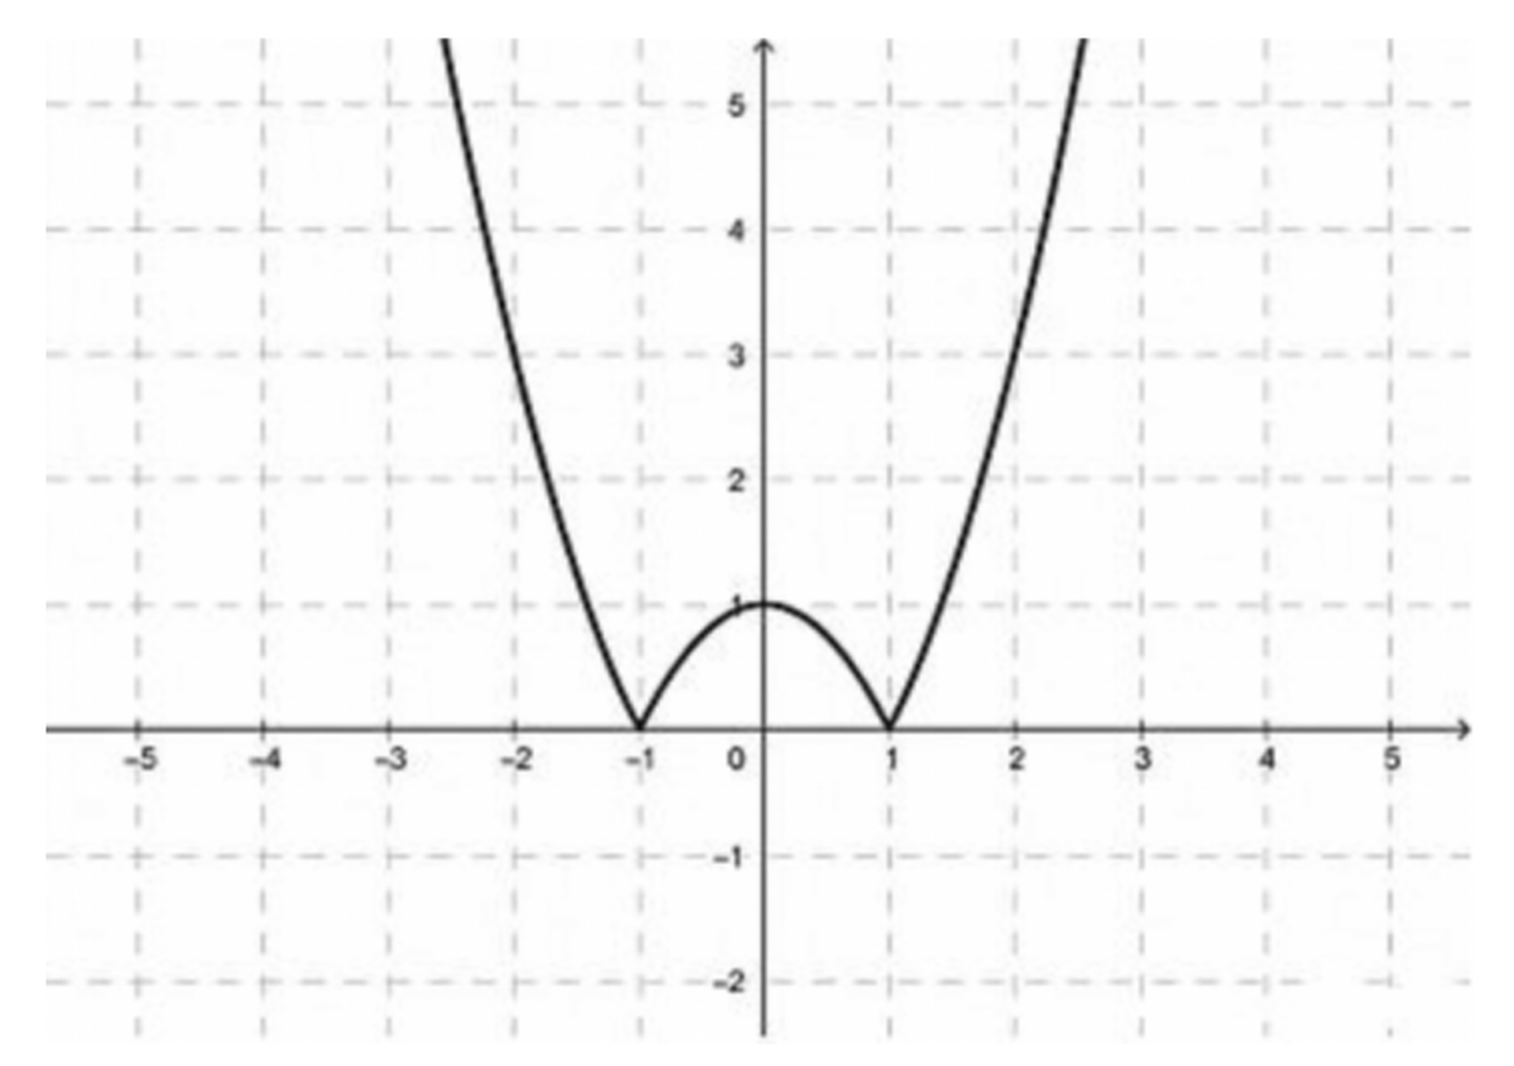
\includegraphics[width=0.55\textwidth]{figures/gao142_q21_para.png}
\end{center}}
\step{(3) 由题意得，$y_1=(2a)^2$，$y_2=(3-a)^2$，}
\step{$y_1<y_2$，即有 $(2a)^2<(3-a)^2$，化简整理得 $(a+3)(a-1)<0$，}
\step{解得实数 $a$ 的取值范围为 $(-3,1)$.}
\solend
\fi

\end{enumerate}

\end{document}
